\documentclass[a4paper,10pt]{article}
\usepackage{fullpage}

\usepackage{natbib}
\usepackage{filecontents}
\usepackage{graphicx}
\usepackage{subcaption}
\usepackage{float}
\usepackage[section]{placeins}
\usepackage{amstext}
\usepackage{amsmath}
\usepackage{amssymb}
\usepackage[colorlinks]{hyperref}
%\usepackage[numbers]{natbib}
%\setlength{\parindent}{1em}
%\setcounter{section}{0}


\begin{document}
\title{\bf Monte Carlo assessment of rheology models via local time-history records}
\author{Ali Akhavan Safaei}
\date{\today}
\maketitle

\begin{figure}[H]
	\centering
	\includegraphics[width=0.5\textwidth]{GeoRefColima.jpg}
	\caption{Location of the selected points to record the time history of flow height, velocity and forces at.}\label{fig:Colima}
\end{figure}
According to the material volume we adopted from \cite{Rupp2006}, $\mathrm{Vol.} = 1.43\times10^5 \ \mathrm{m}^3$, here we are varying it by $\pm15\%$. Therefore, volume range would be: $\mathrm{Vol.} \in [1.21 \ \ 1.64] \times10^5 \ \mathrm{m}^3$. The stochasticity of each rheology model's parameter space is table \ref{tab:Para}. 
\begin{table}[H]
\begin{center}
\caption{ Parameter spaces and their ranges of variations for Monte Carlo simulations.}
\label{tab:Para}
	\begin{tabular}{lc}
    \hline
    \textbf{Rheology model} & \textbf{Parameter space and uncertainty range} \\
    \hline
    Mohr-Coulomb & $\phi_{\mathrm{bed}} \in [15^{\circ} \ \ 37^{\circ}], \ \phi_{\mathrm{int}}\in[35^{\circ} \ \ 45^{\circ}]$ \\
    Voellmy-Salm & $\mu\in[0.2 \ \ 0.9], \ \ \xi\in[50 \ \ 5000]$ m/s \\
    Pouliquen-Forterre & $\phi_1\in[15^{\circ} \ \ 38^{\circ}], \ \ \phi_2\in[39^{\circ} \ \ 45^{\circ}], \ \ \beta\in[0.1 \ \ 0.85]$ \\
    \hline
	\end{tabular}
\end{center}
\end{table}
In section \ref{sec:MV_comb}, we can see the mean values of flow height and velocity records (Fig. \ref{fig:M_HeiVelall}), net force records \textit{i.e.} $\Vert F_{\mathrm{Driv.}} - F_{\mathrm{Res.}} \Vert$ (Fig. \ref{fig:M_Fnet}), records of gravitatonal and bed friction forces (Fig. \ref{fig:M_Fgball}) and records of other ``model-specific'' resisting forces (Fig. \ref{fig:M_FoCall}) at all 10 locations (the pile location is not included) so that we can visually make comparison between the results of each model simulation at all of these locations. In section \ref{sec:MV_loc}, we can see the mean value of flow heights and velocities records at each location for all three rheology models (Fig. \ref{fig:MFHVR_L123}, \ref{fig:MFHVR_L456}, \ref{fig:MFHVR_L789} and \ref{fig:MFHVR_L1011}).

Finally, in section \ref{sec:NetF}, we have the statistical investigations for the recorded net force at each location (11 locations) for all rheology models so that we can locally make visual comparison between the mean value, highest and lowest 5\% bounds of variations for rheology models (Fig. \ref{fig:NF123}, \ref{fig:NF456}, \ref{fig:NF789} and \ref{fig:NF1011}).

\section{Mean Values}\label{sec:MVs}

\subsection{Combined Records}\label{sec:MV_comb}
\begin{figure}[H]

	\begin{minipage}[b]{0.5\linewidth}
	\centering
    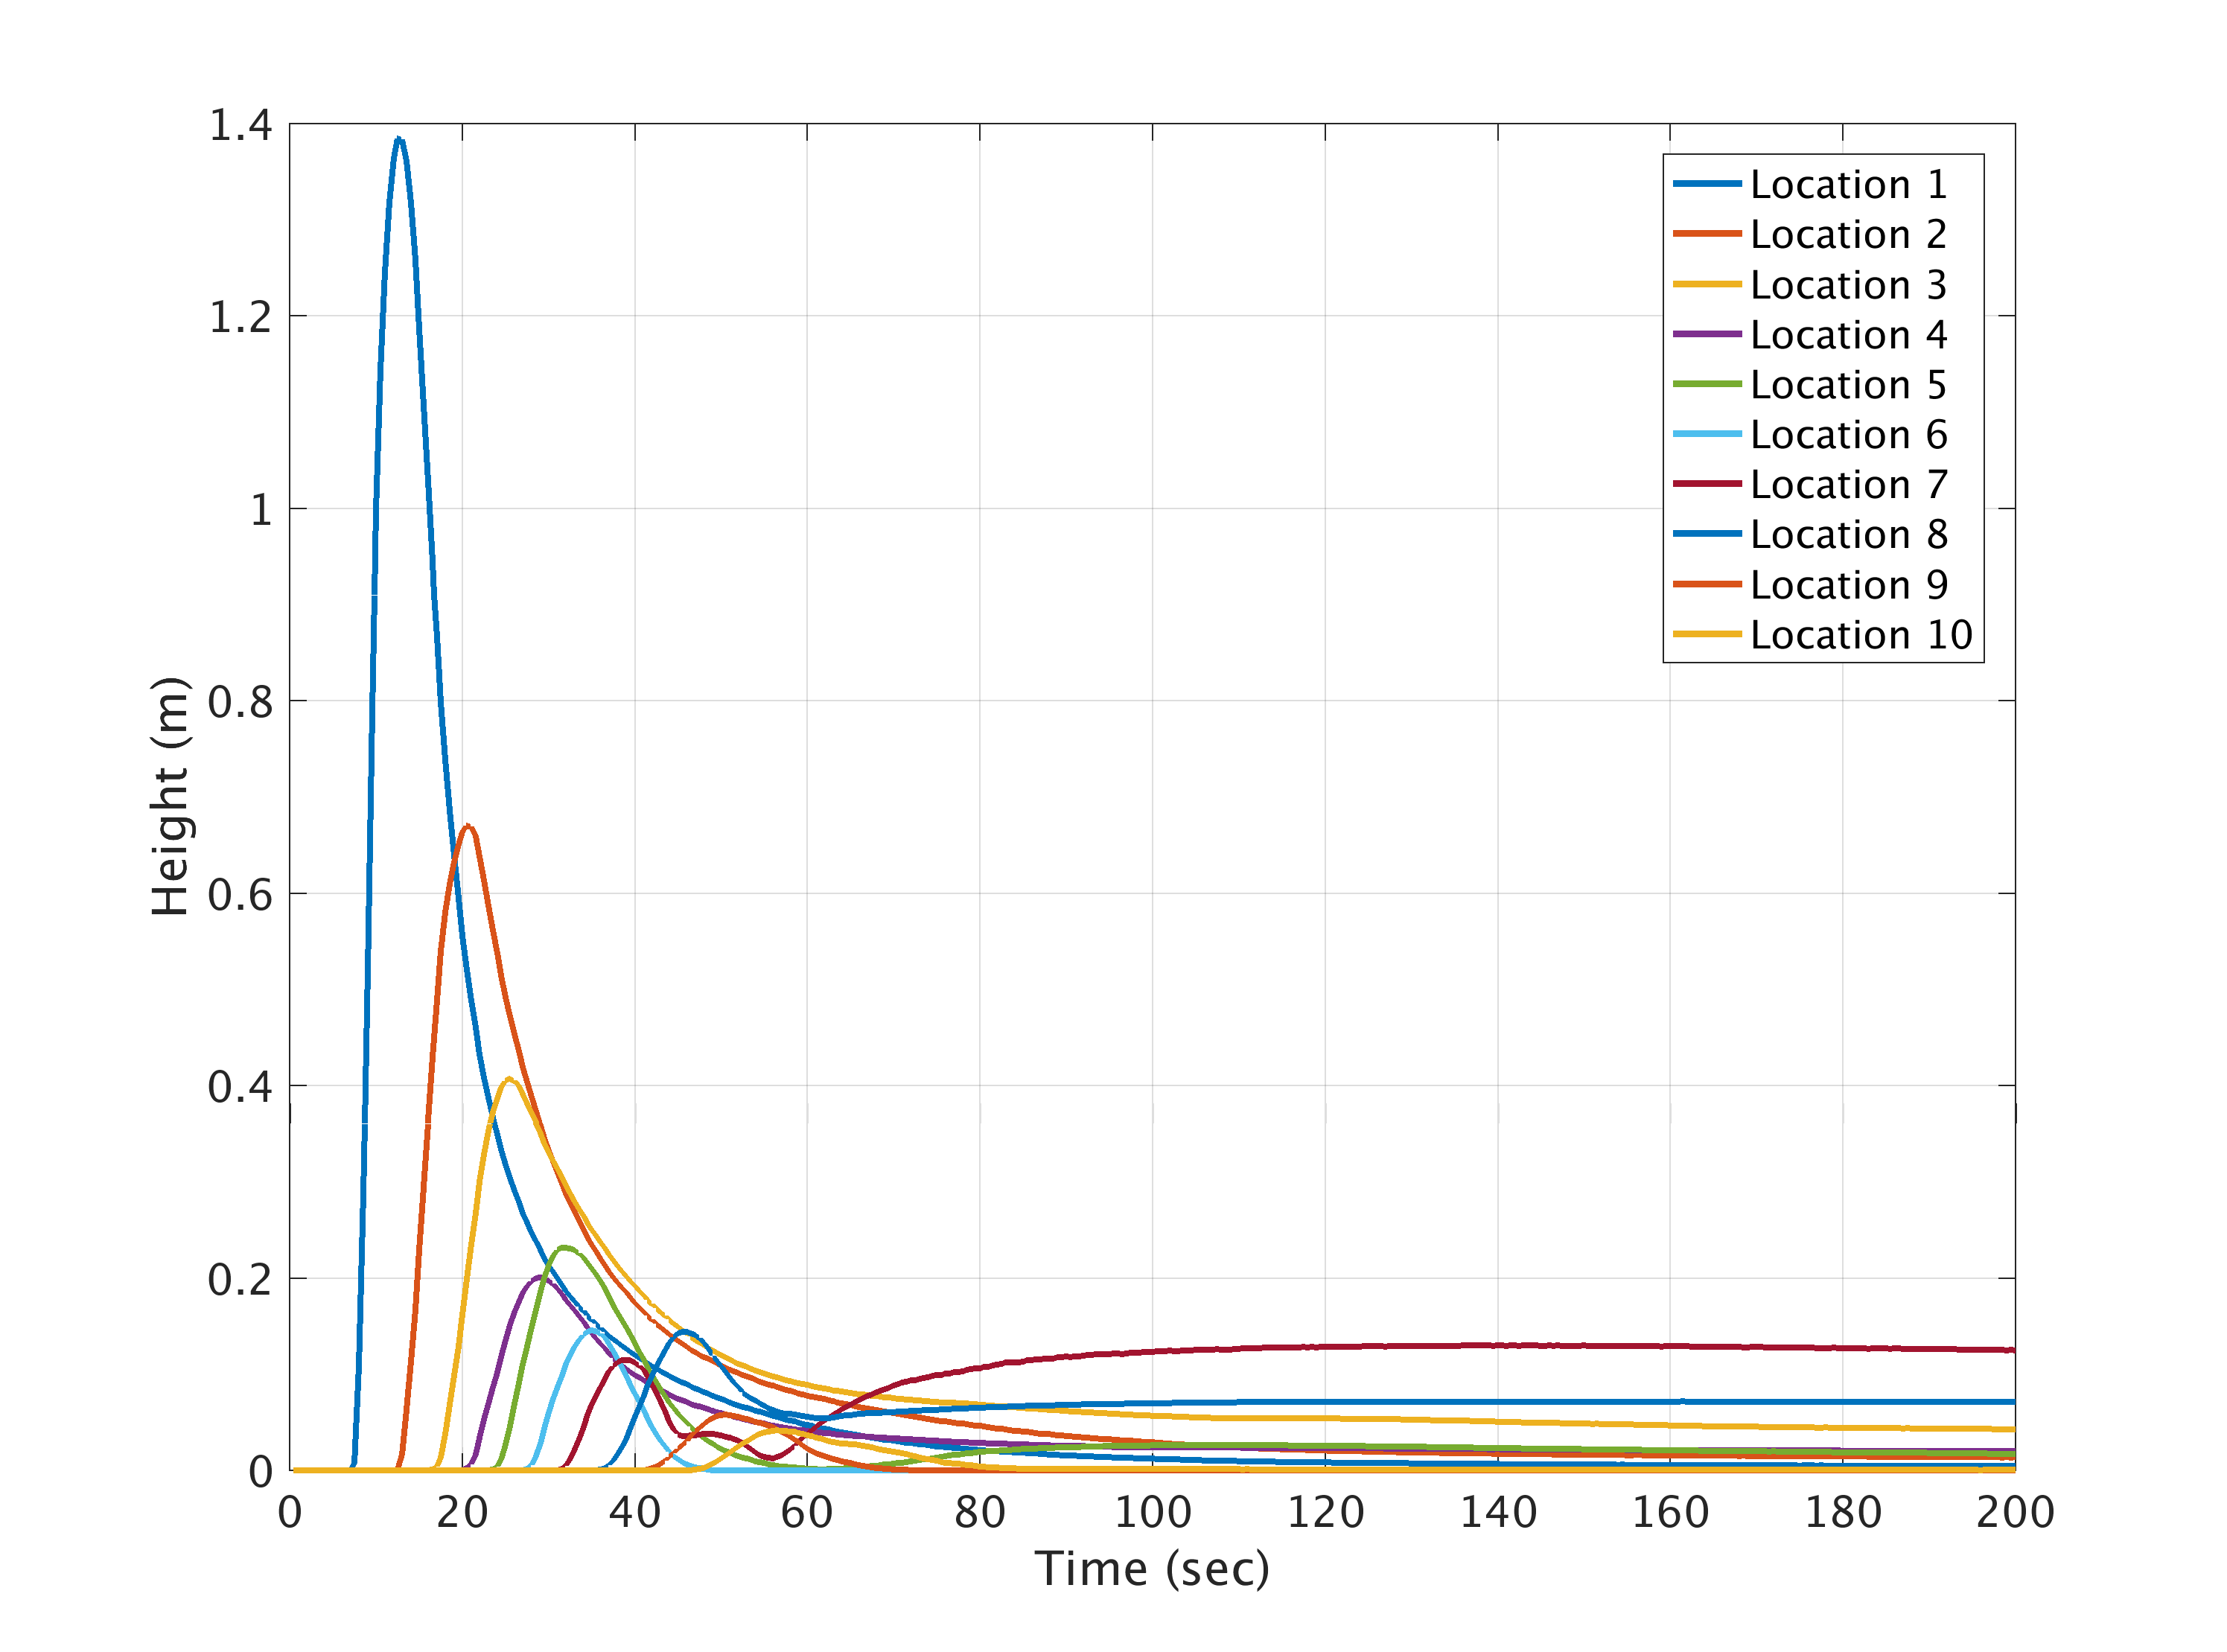
\includegraphics[width=1\textwidth]{MeansAll/HC_all.png}     
        \subcaption{Flow Height Records, Mohr-Coulomb.}
        \label{fig:M_HCall}
	\end{minipage}
	\begin{minipage}[b]{0.5\linewidth}
	\centering
    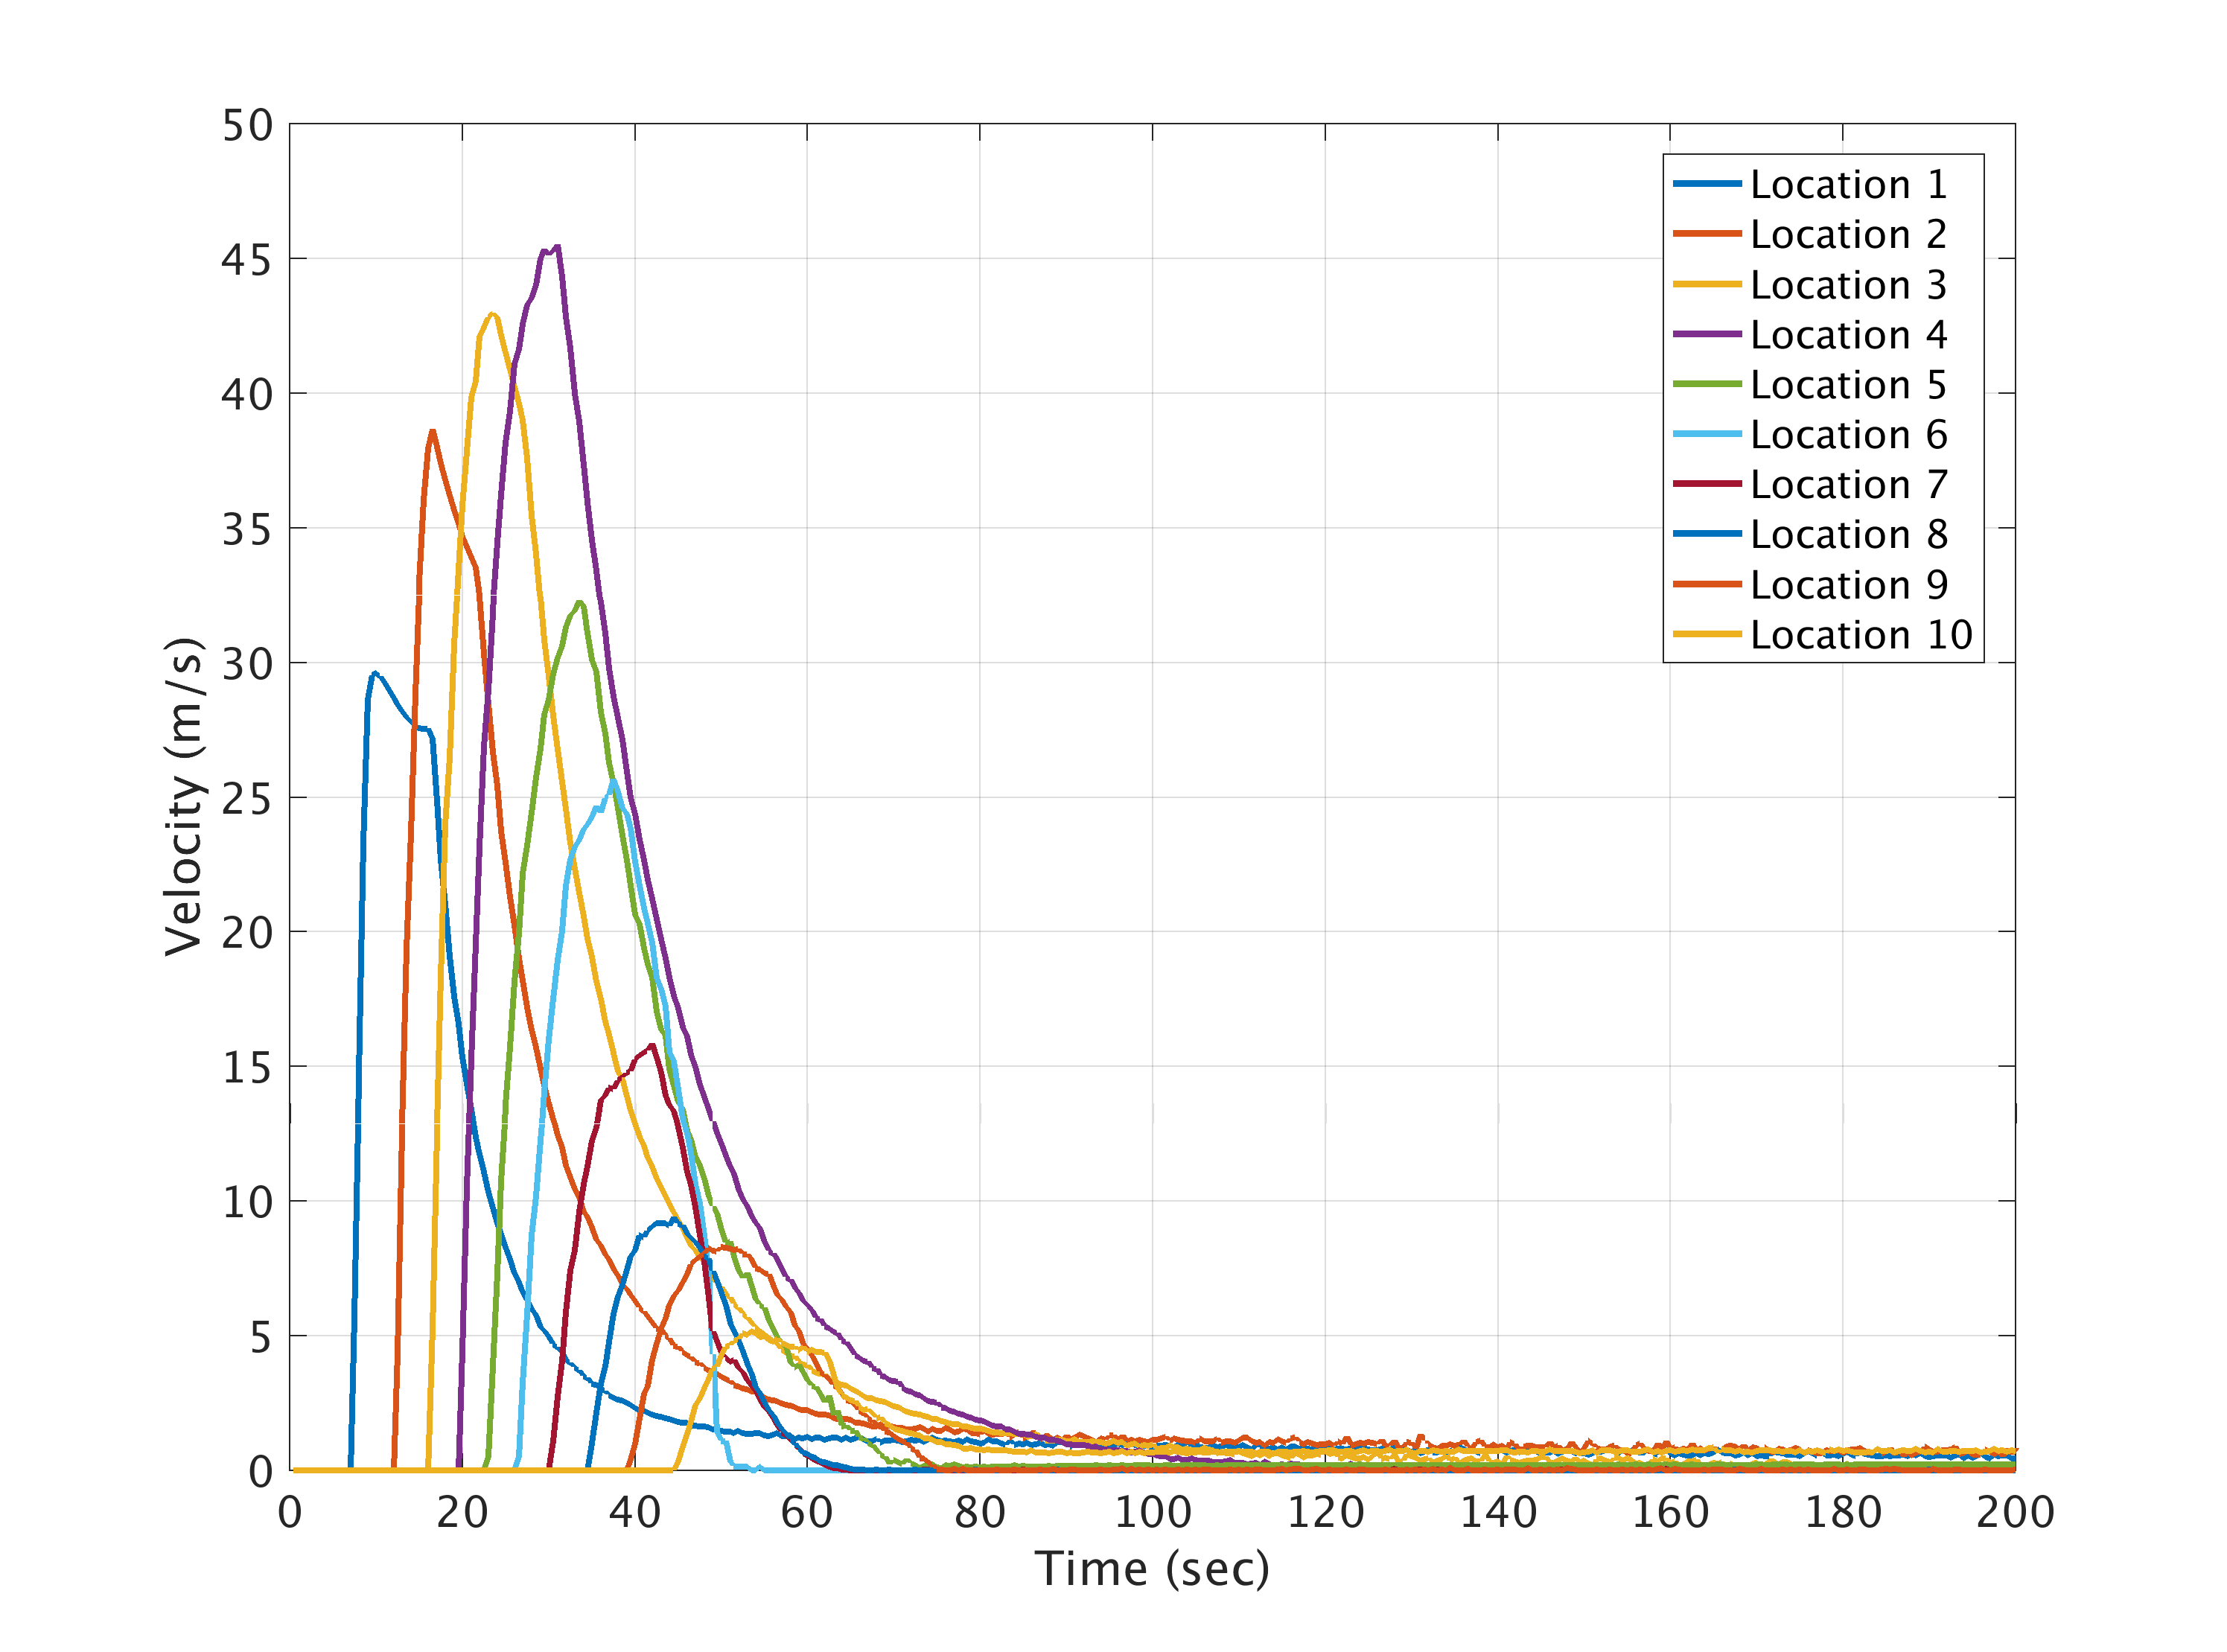
\includegraphics[width=1\textwidth]{MeansAll/VC_all.png}     
        \subcaption{Flow Velocity Records, Mohr-Coulomb.}
        \label{fig:M_VCall}
	\end{minipage}
	
	\begin{minipage}[b]{0.5\linewidth}
	\centering
    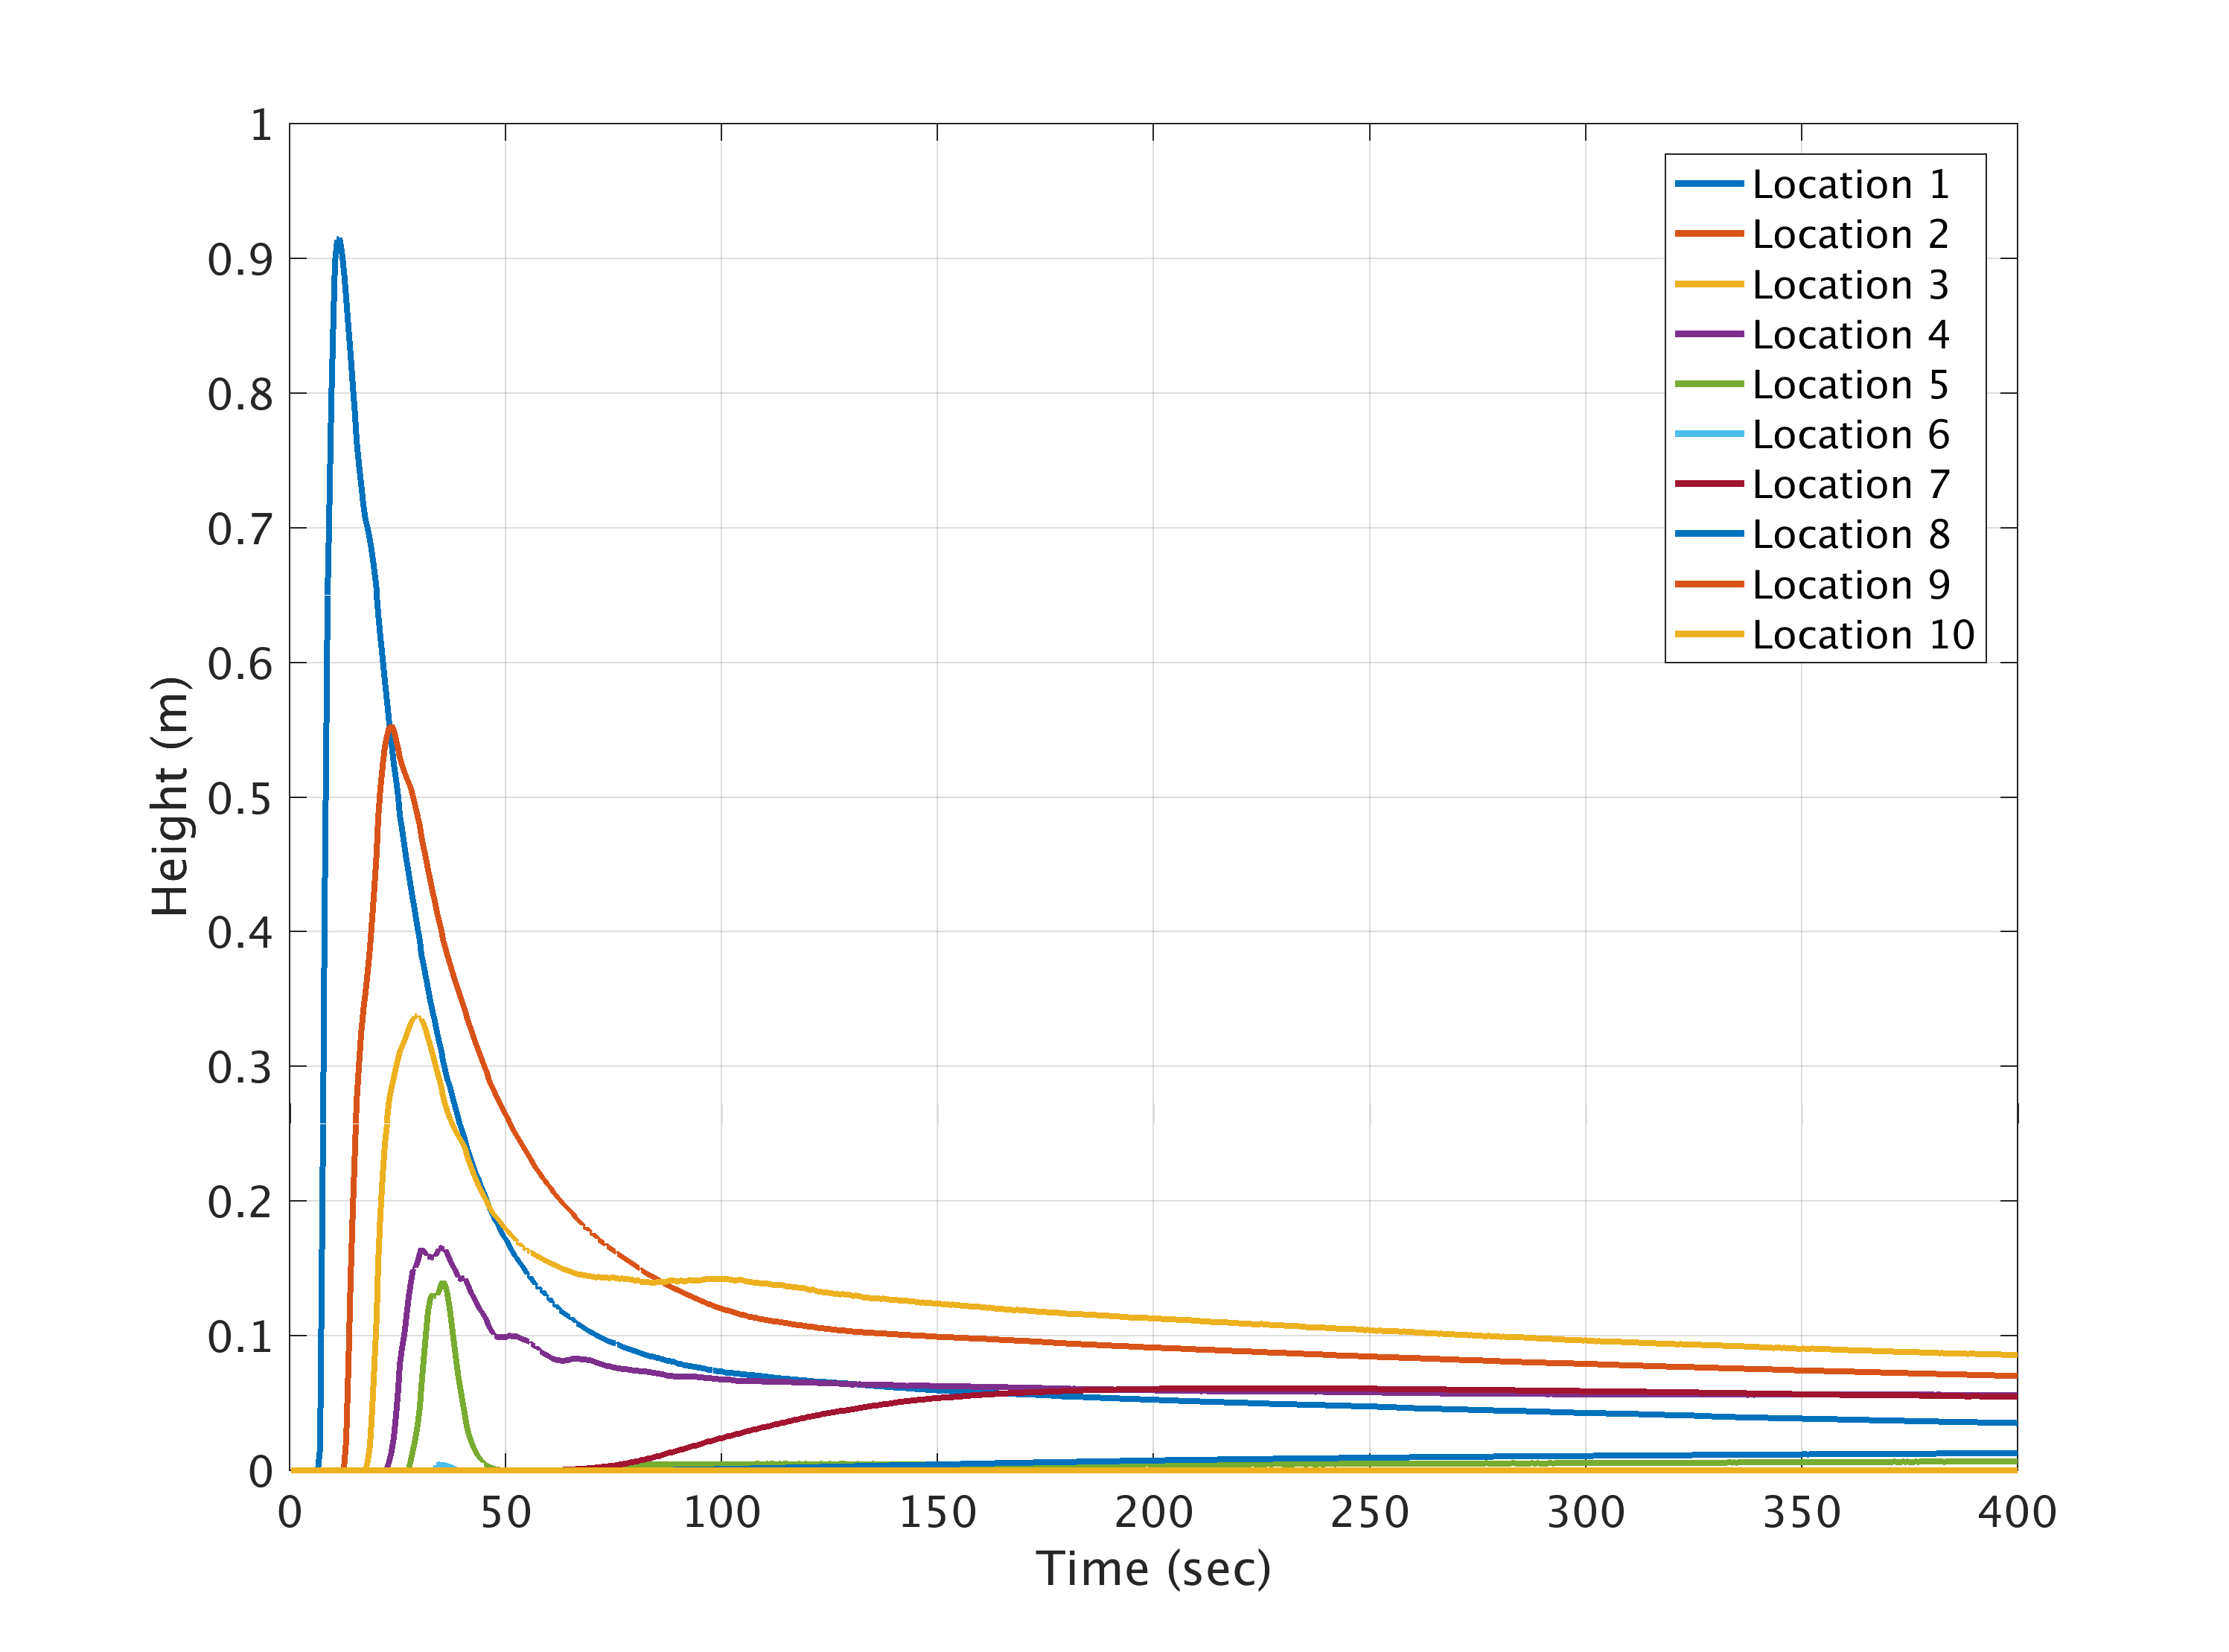
\includegraphics[width=1\textwidth]{MeansAll/HP_all.png}
        \subcaption{Flow Height Records, Pouliquen-Forterre.}
        \label{fig:M_HPall}
	\end{minipage}
	\begin{minipage}[b]{0.5\linewidth}
	\centering
    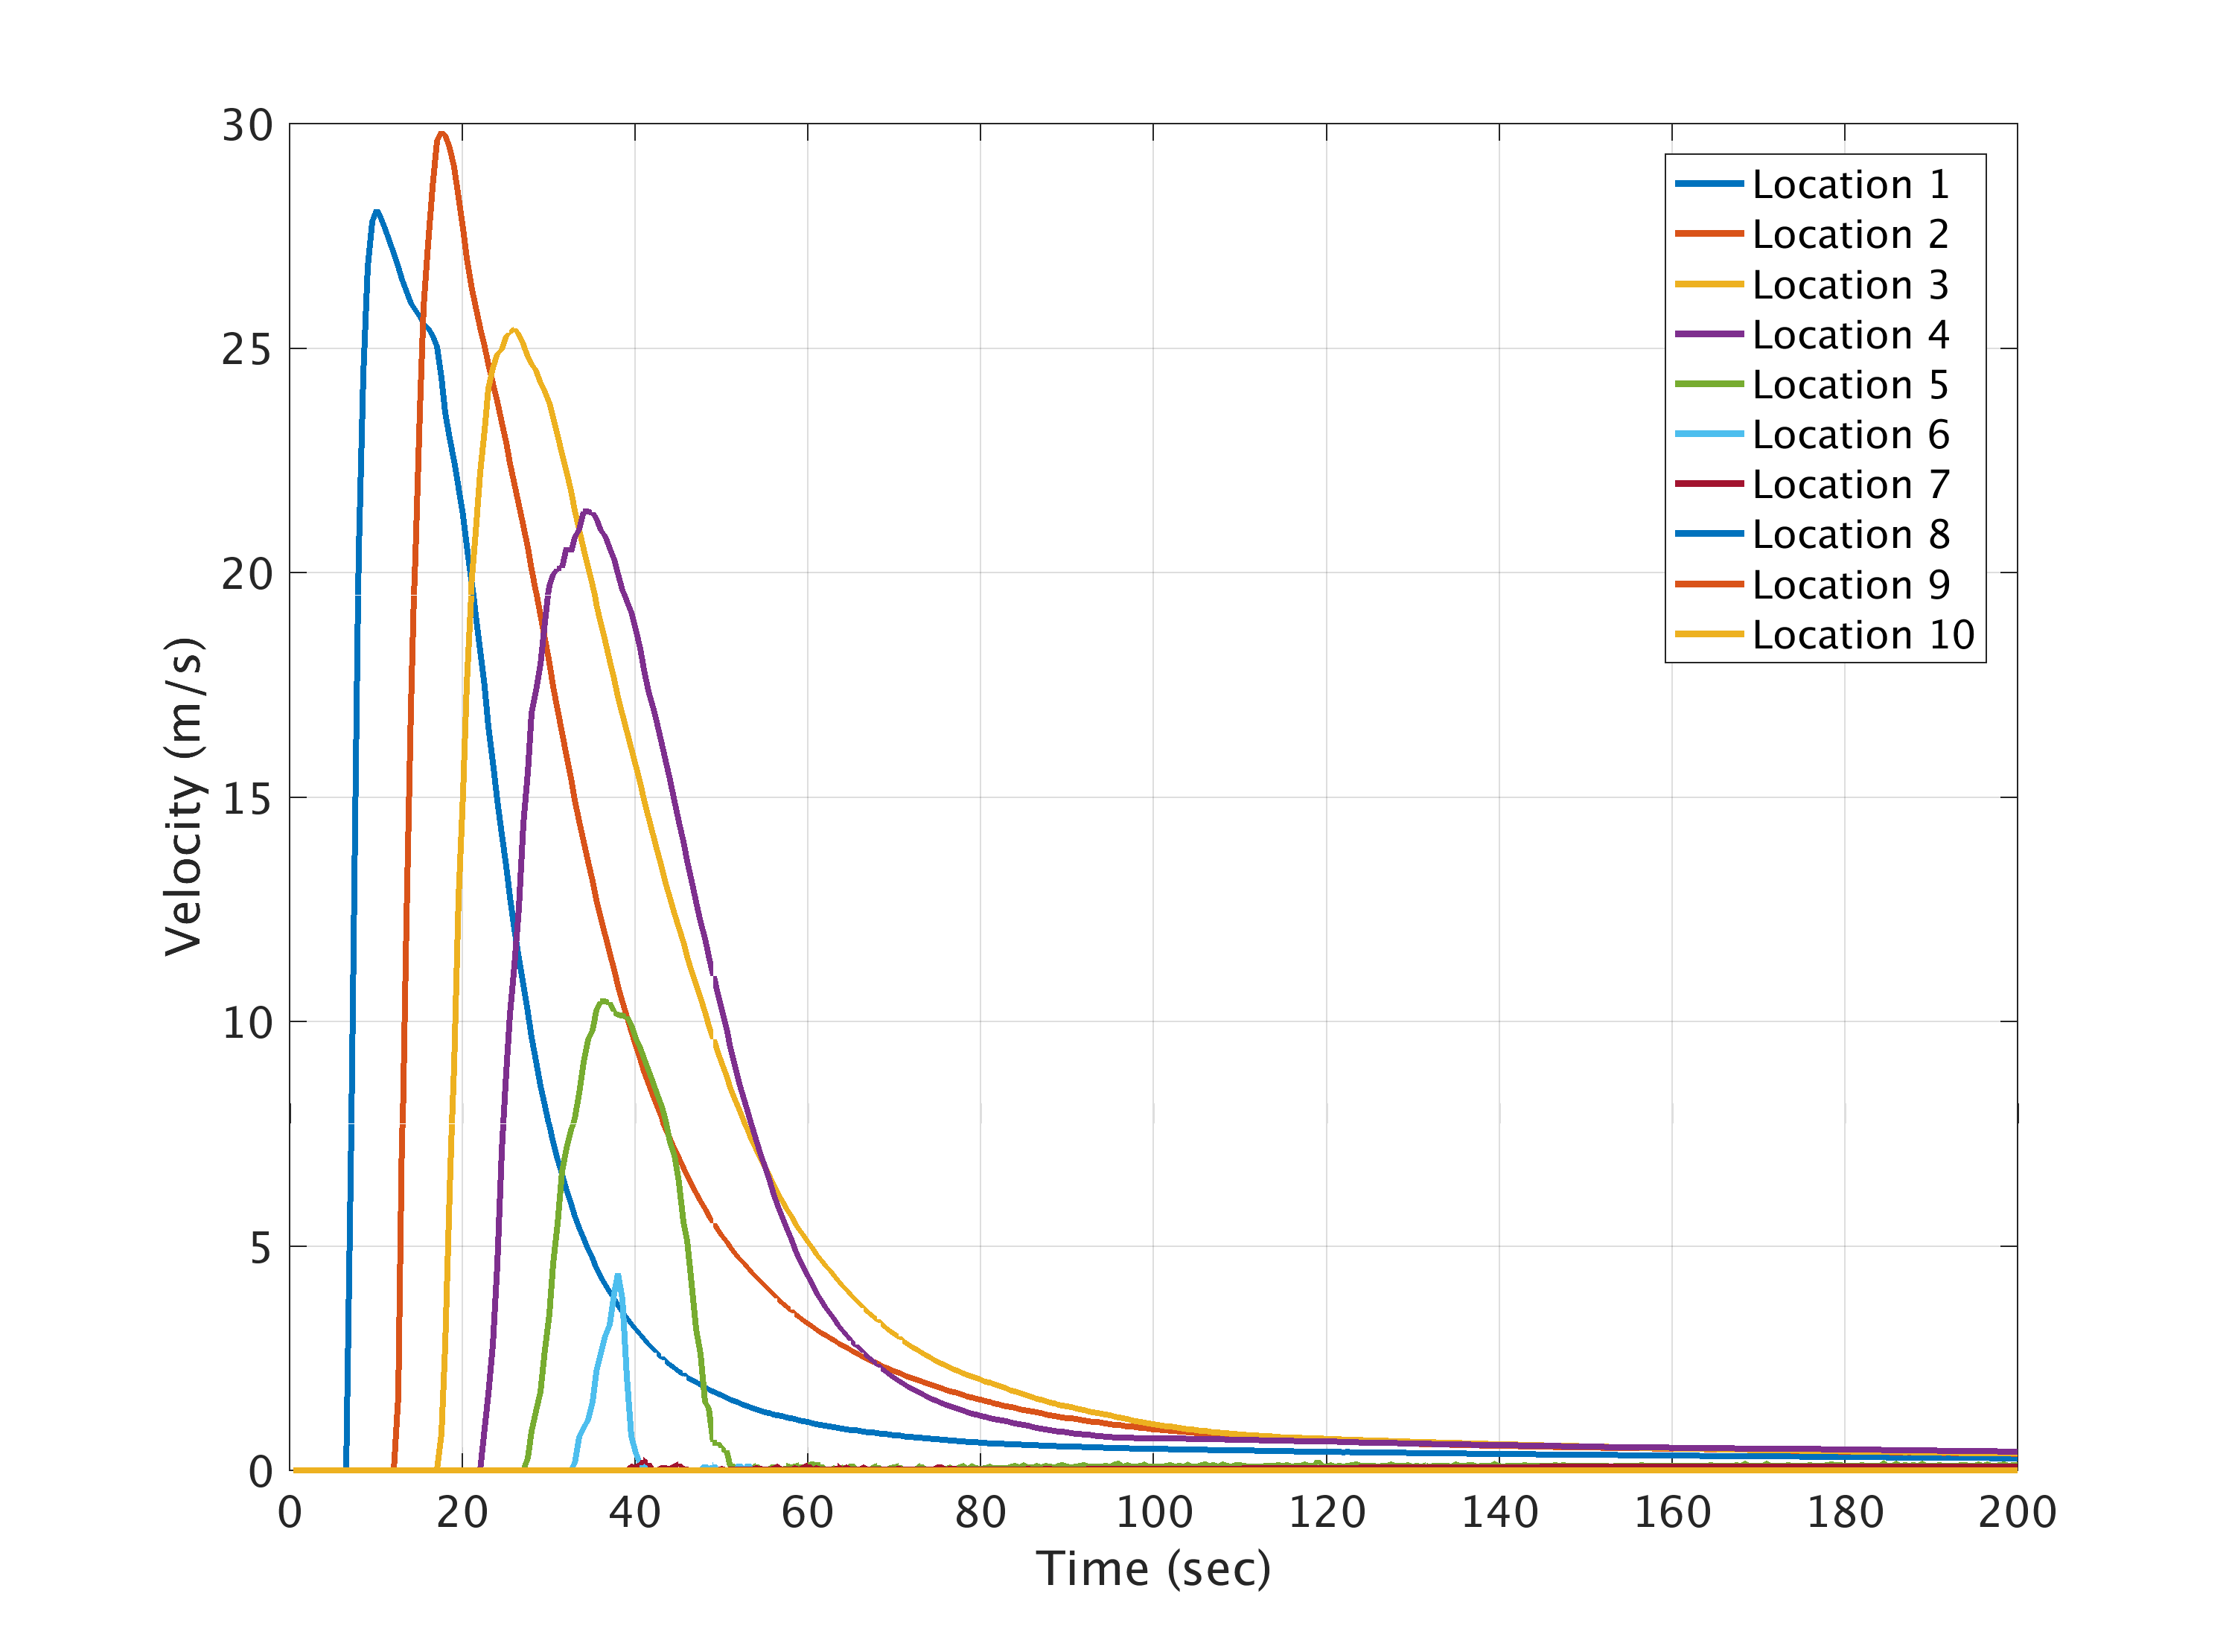
\includegraphics[width=1\textwidth]{MeansAll/VP_all.png}
        \subcaption{Flow Velocity Records, Pouliquen-Forterre.}
        \label{fig:M_VPall}
	\end{minipage}
	
	\begin{minipage}[b]{0.5\linewidth}
	\centering
    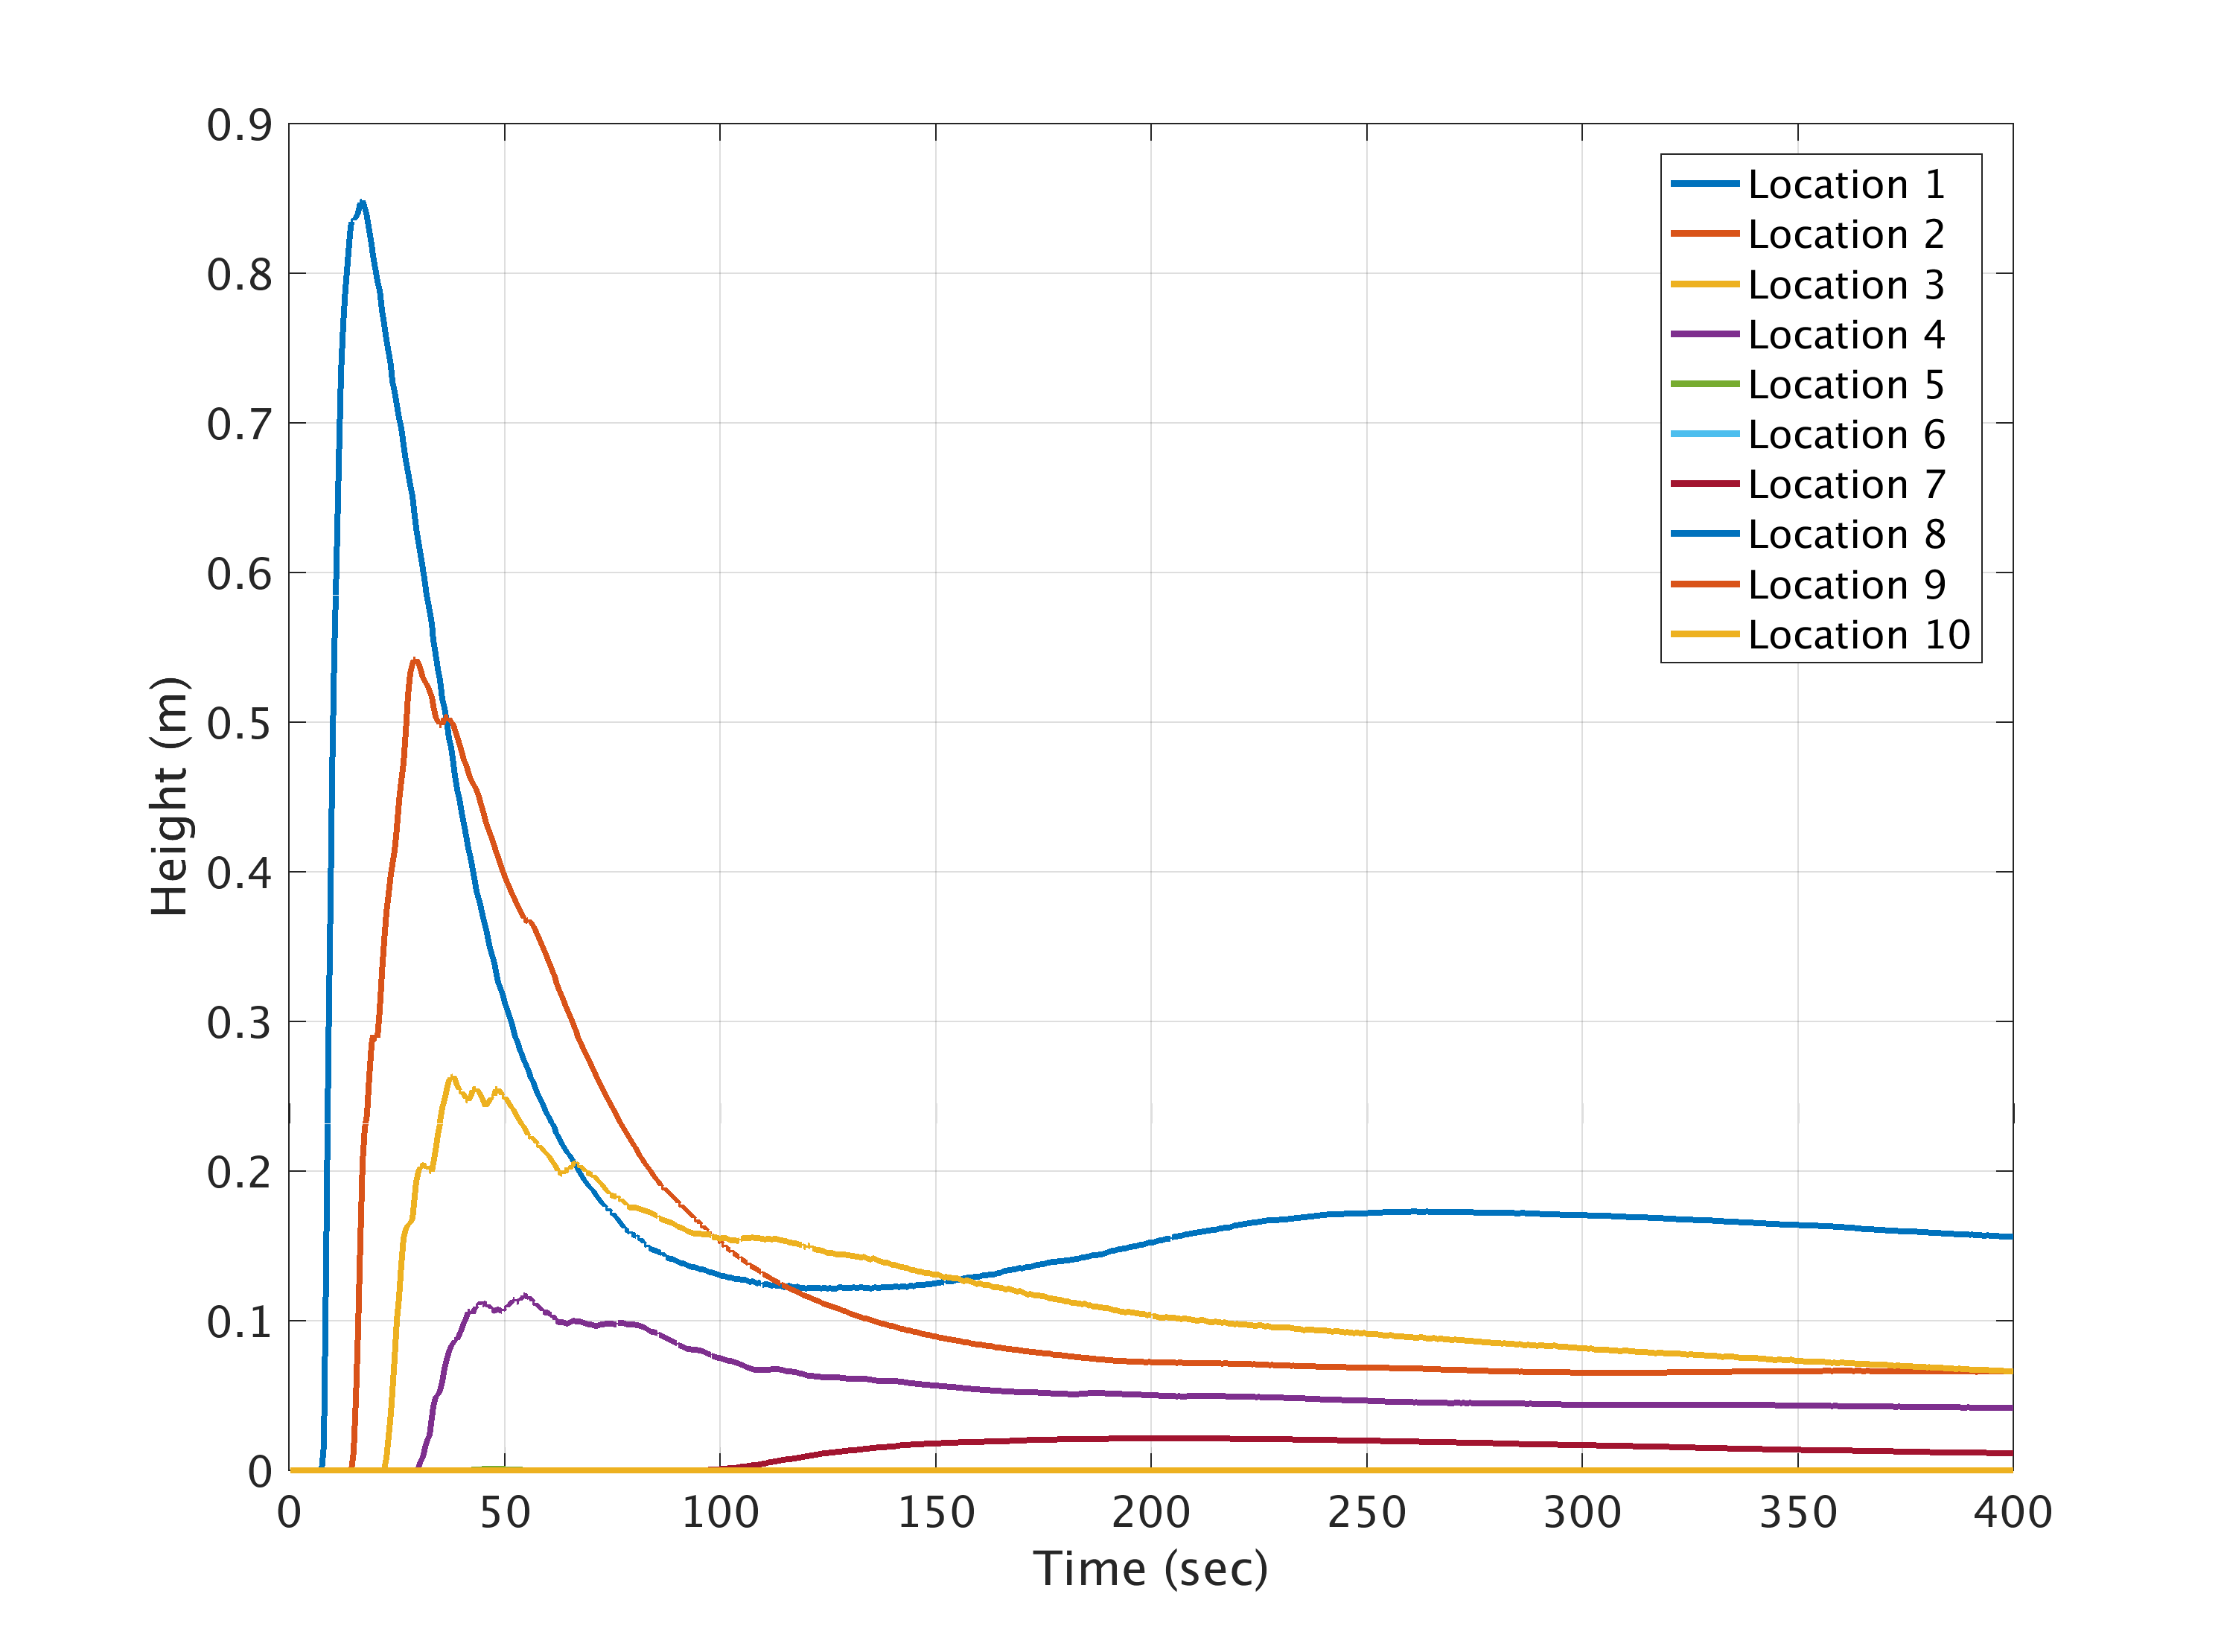
\includegraphics[width=1\textwidth]{MeansAll/HV_all.png}
        \subcaption{Flow Height Records, Voellmy-Salm.}
        \label{fig:M_HVall}
	\end{minipage}
	\begin{minipage}[b]{0.5\linewidth}
	\centering
    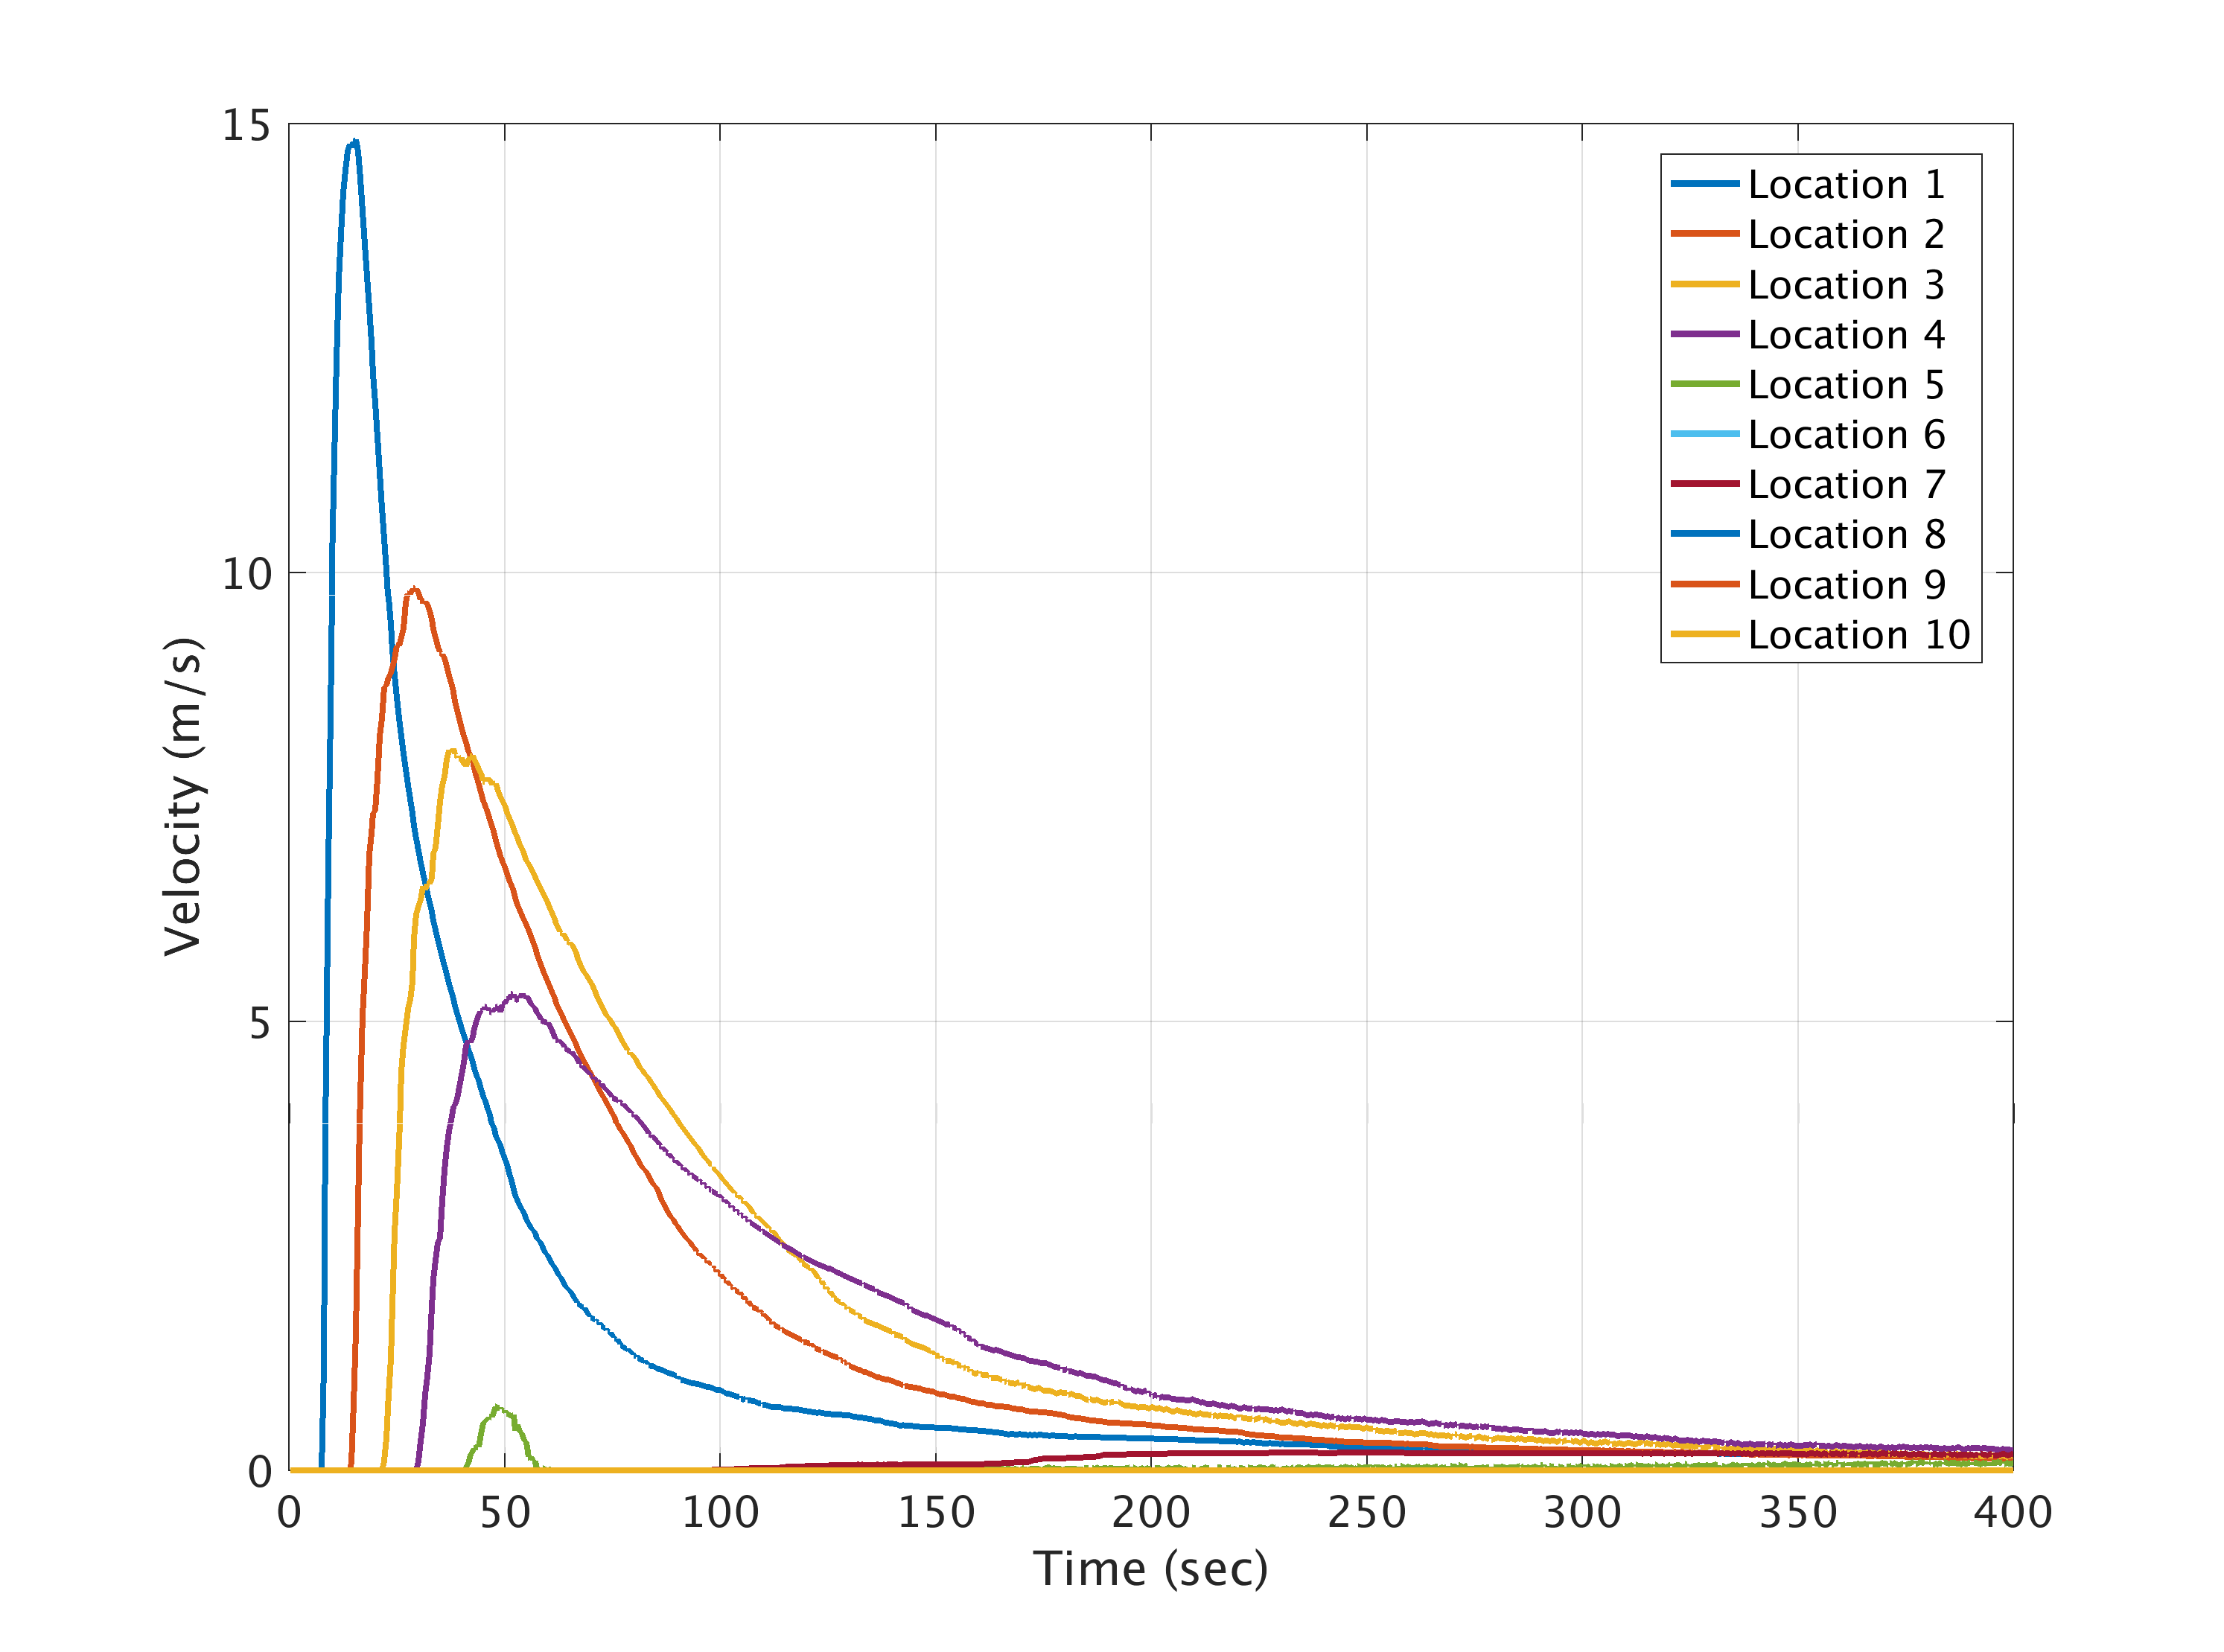
\includegraphics[width=1\textwidth]{MeansAll/VV_all.png}
        \subcaption{Flow Velocity Records, Voellmy-Salm.}
        \label{fig:M_VVall}
	\end{minipage}
	
	\caption{Mean Values of flow height and velocity records at all the specified locations.}\label{fig:M_HeiVelall}	
\end{figure}

According to Figures \ref{fig:M_HCall}, \ref{fig:M_HPall} and \ref{fig:M_HVall}, maximum flow height occurs when the rheology model is more of frictional (Mohr-Coulomb and Pouliquen-Forterre) than viscose (Voellmy-Salm), however, these plots show that the material accumulation \textit{i.e.} constant flow heights at very low velocities, is mostly occuring when the rheology model is Voellmy-Salm and Pouliquen-Forterre. In other words, the flowing material doesn't get far downhill so that we see many not-wetted locations mostly in Voellmy-Salm model and then in Pouliquen-Forterre model. 

\begin{figure}[H]

	\begin{minipage}[b]{0.5\linewidth}
	\centering
    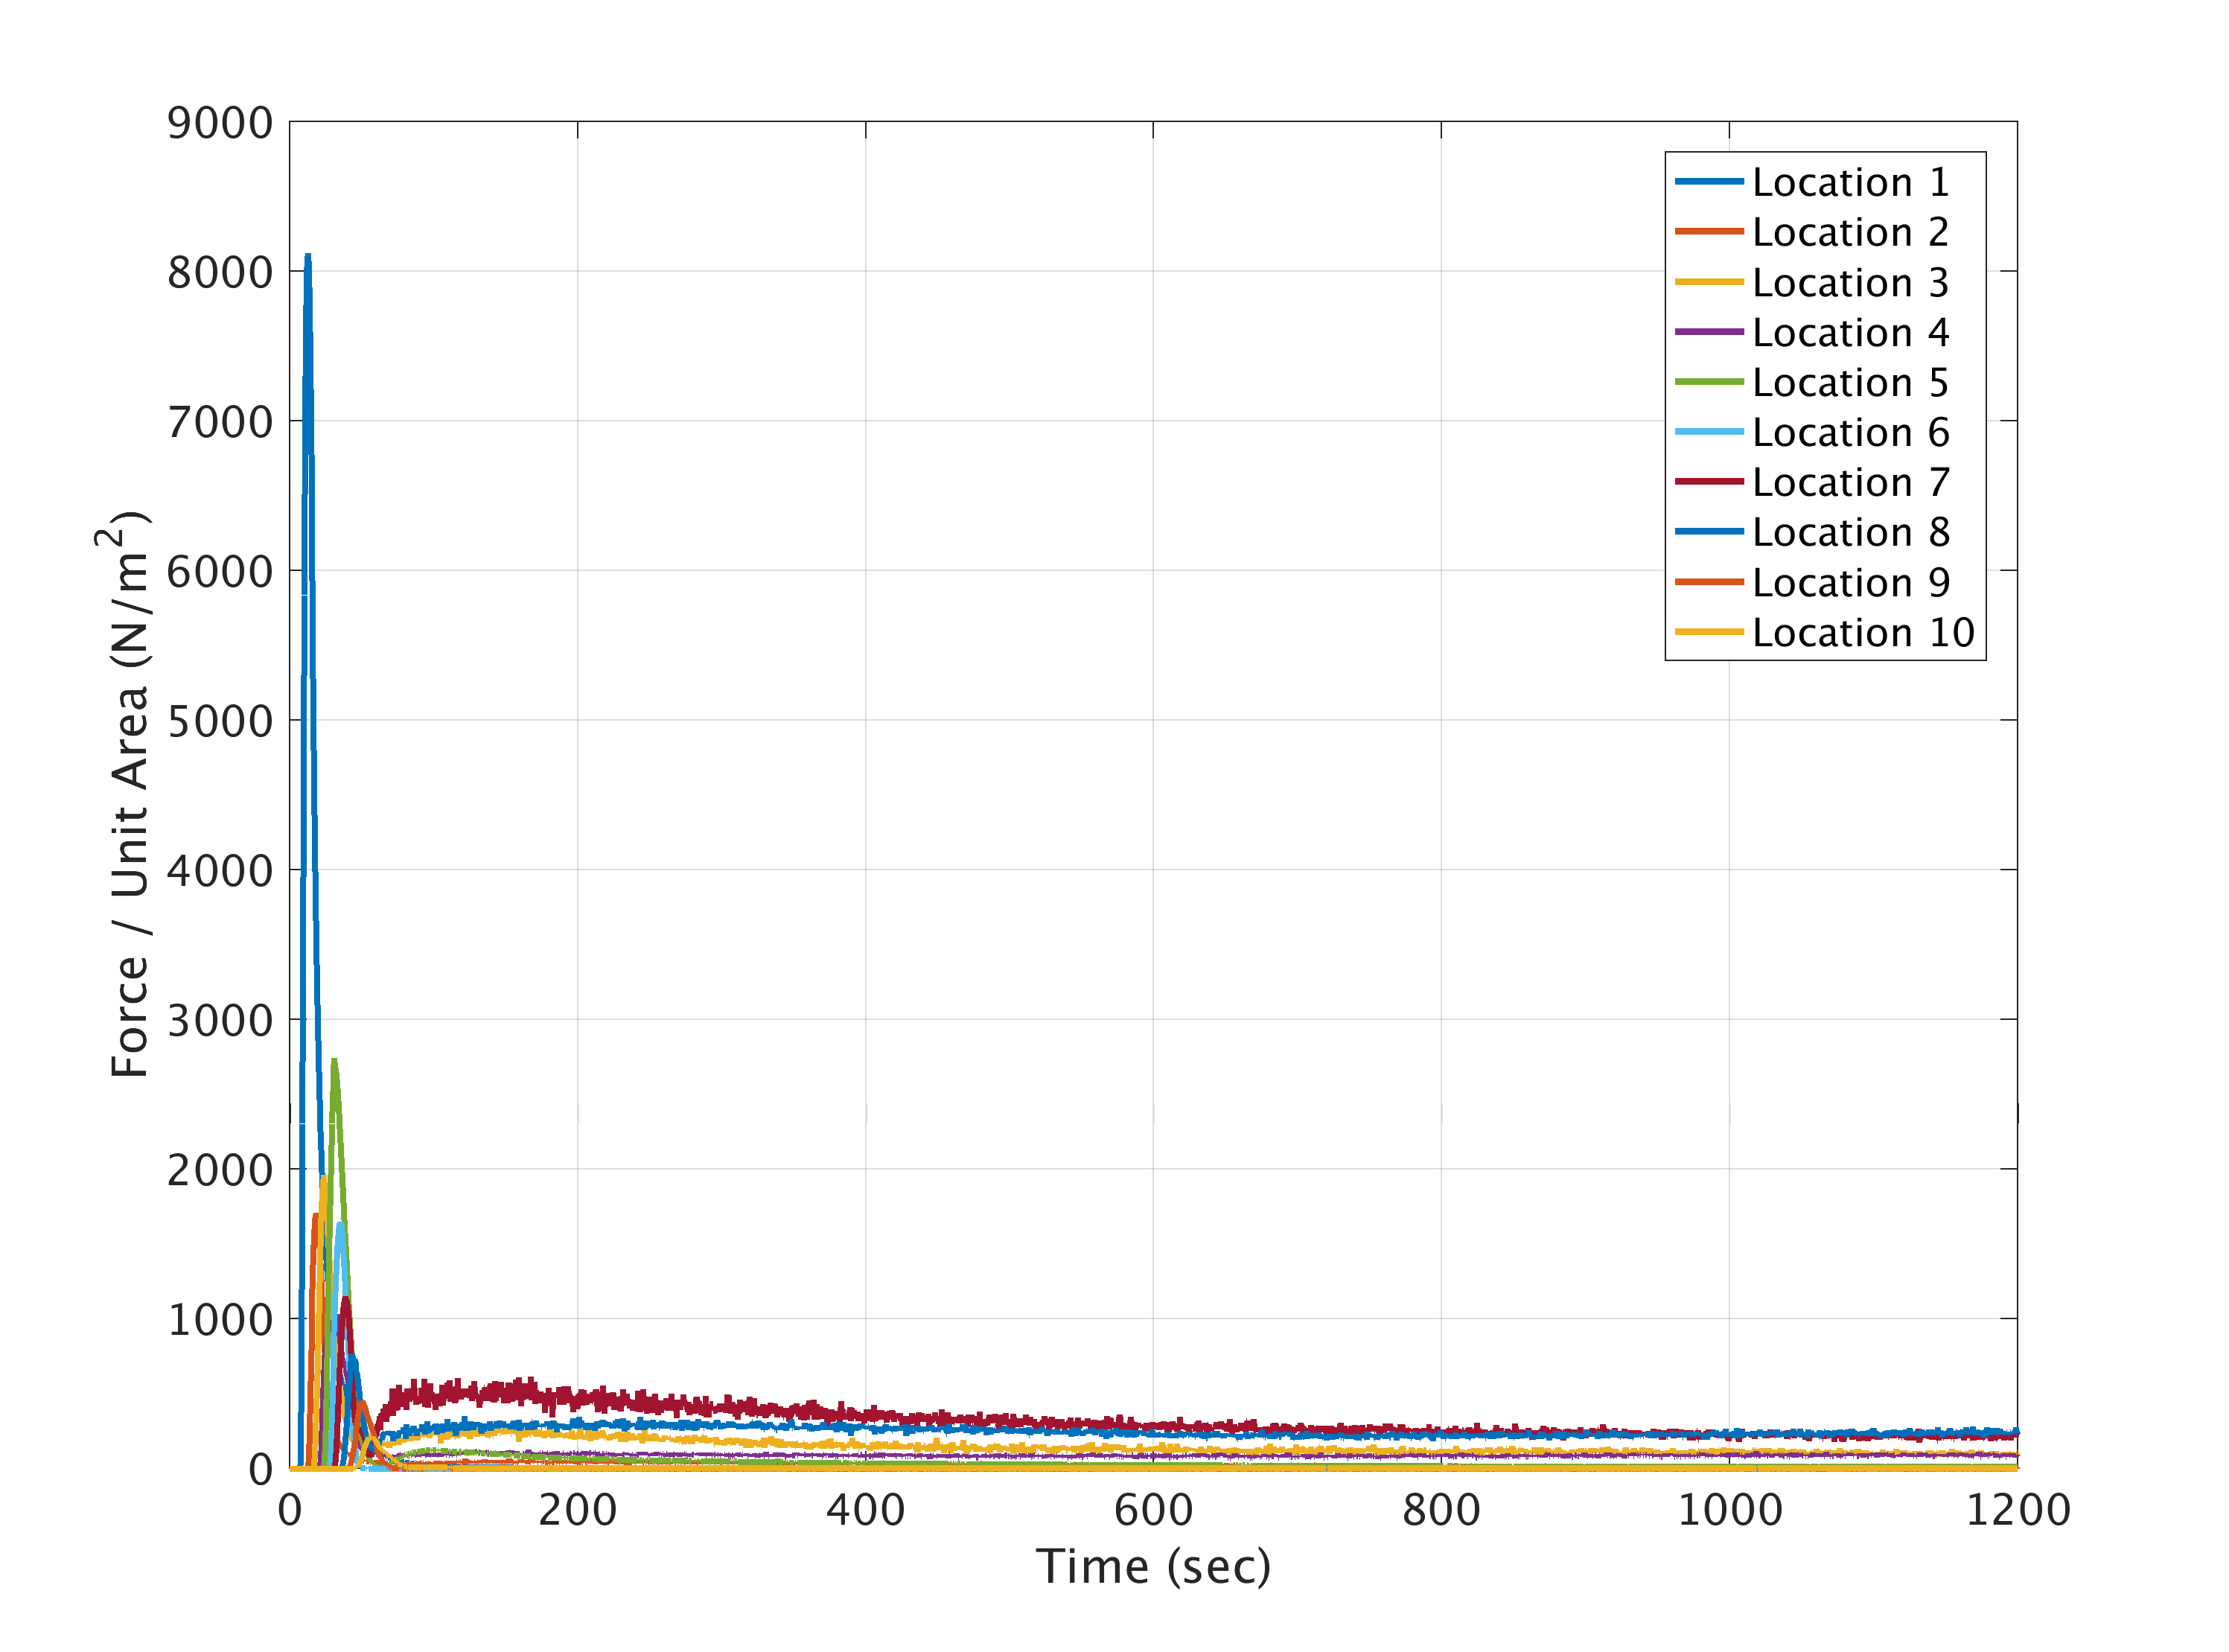
\includegraphics[width=1\textwidth]{MeansAll/FnetC.png}     
        \subcaption{Net Force Records, Mohr-Coulomb.}
        \label{fig:M_FnC}
	\end{minipage}
	\begin{minipage}[b]{0.5\linewidth}
	\centering
    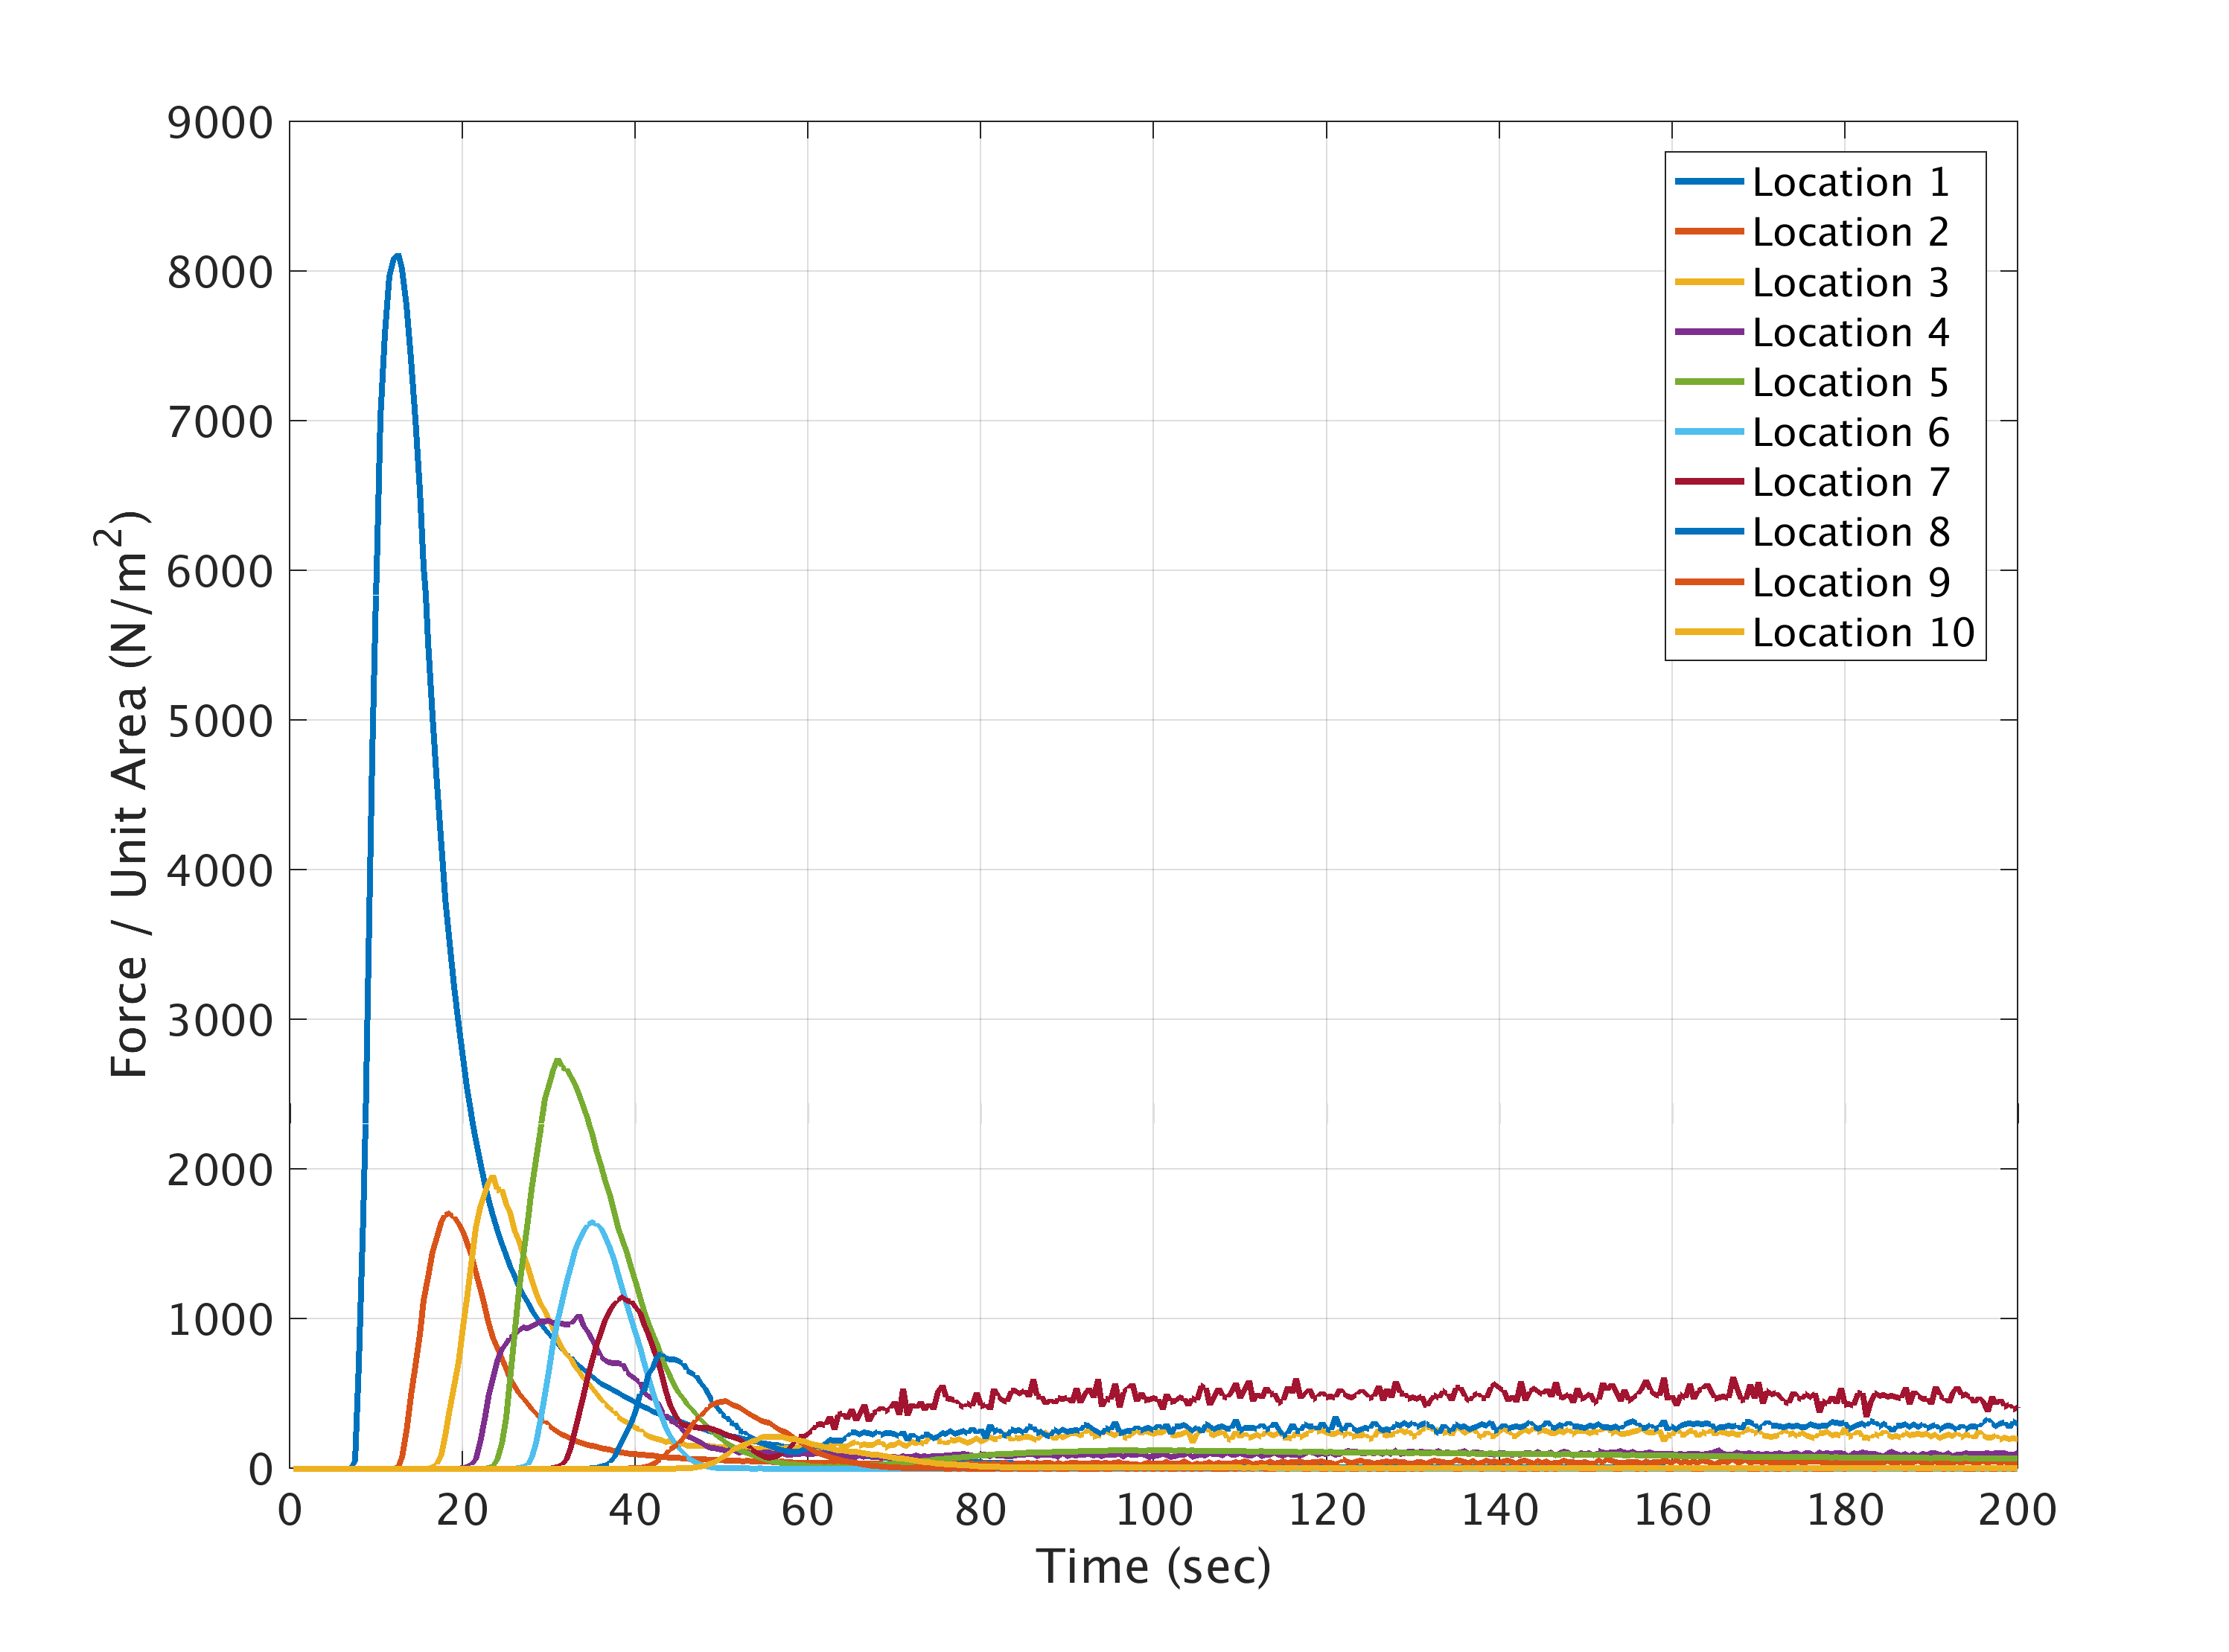
\includegraphics[width=1\textwidth]{MeansAll/FnetC_0-200.png}     
        \subcaption{Zoomed view of Fig. (\ref{fig:M_FnC}).}
        \label{fig:M_FnCz}
	\end{minipage}
	
	\begin{minipage}[b]{0.5\linewidth}
	\centering
    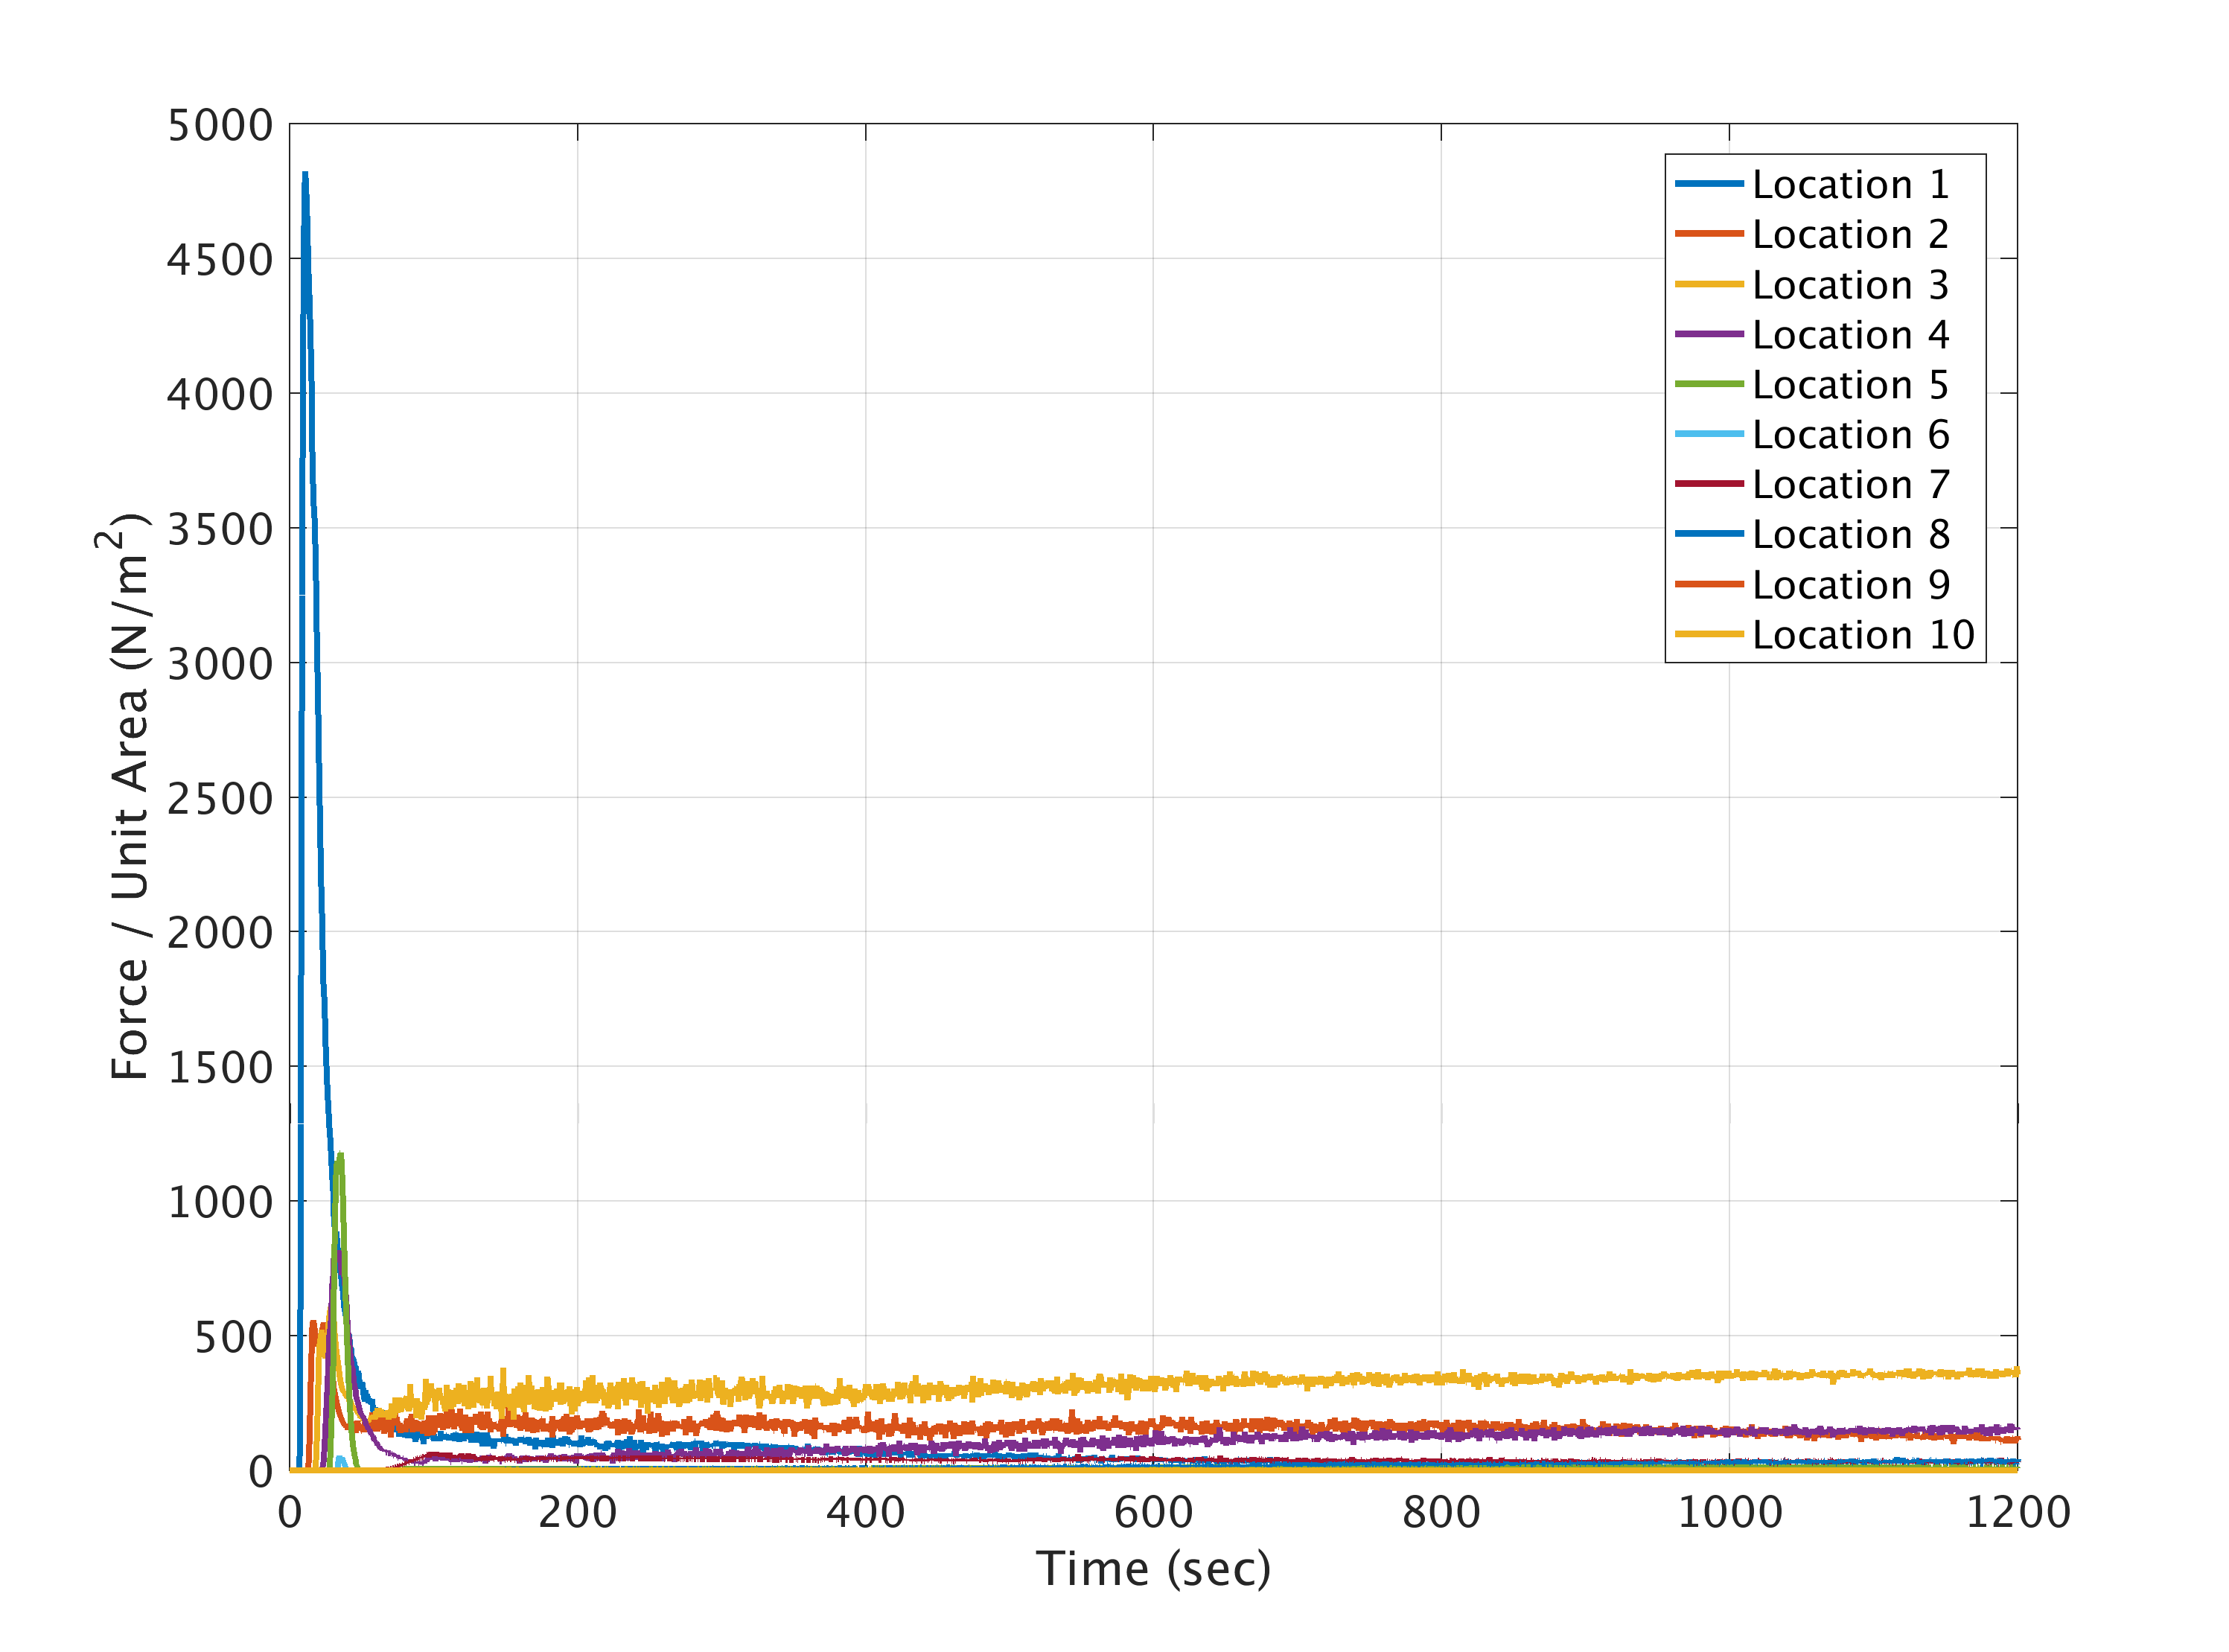
\includegraphics[width=1\textwidth]{MeansAll/FnetP.png}
        \subcaption{Net Force Records, Pouliquen-Forterre.}
        \label{fig:M_FnP}
	\end{minipage}	
	\begin{minipage}[b]{0.5\linewidth}
	\centering
    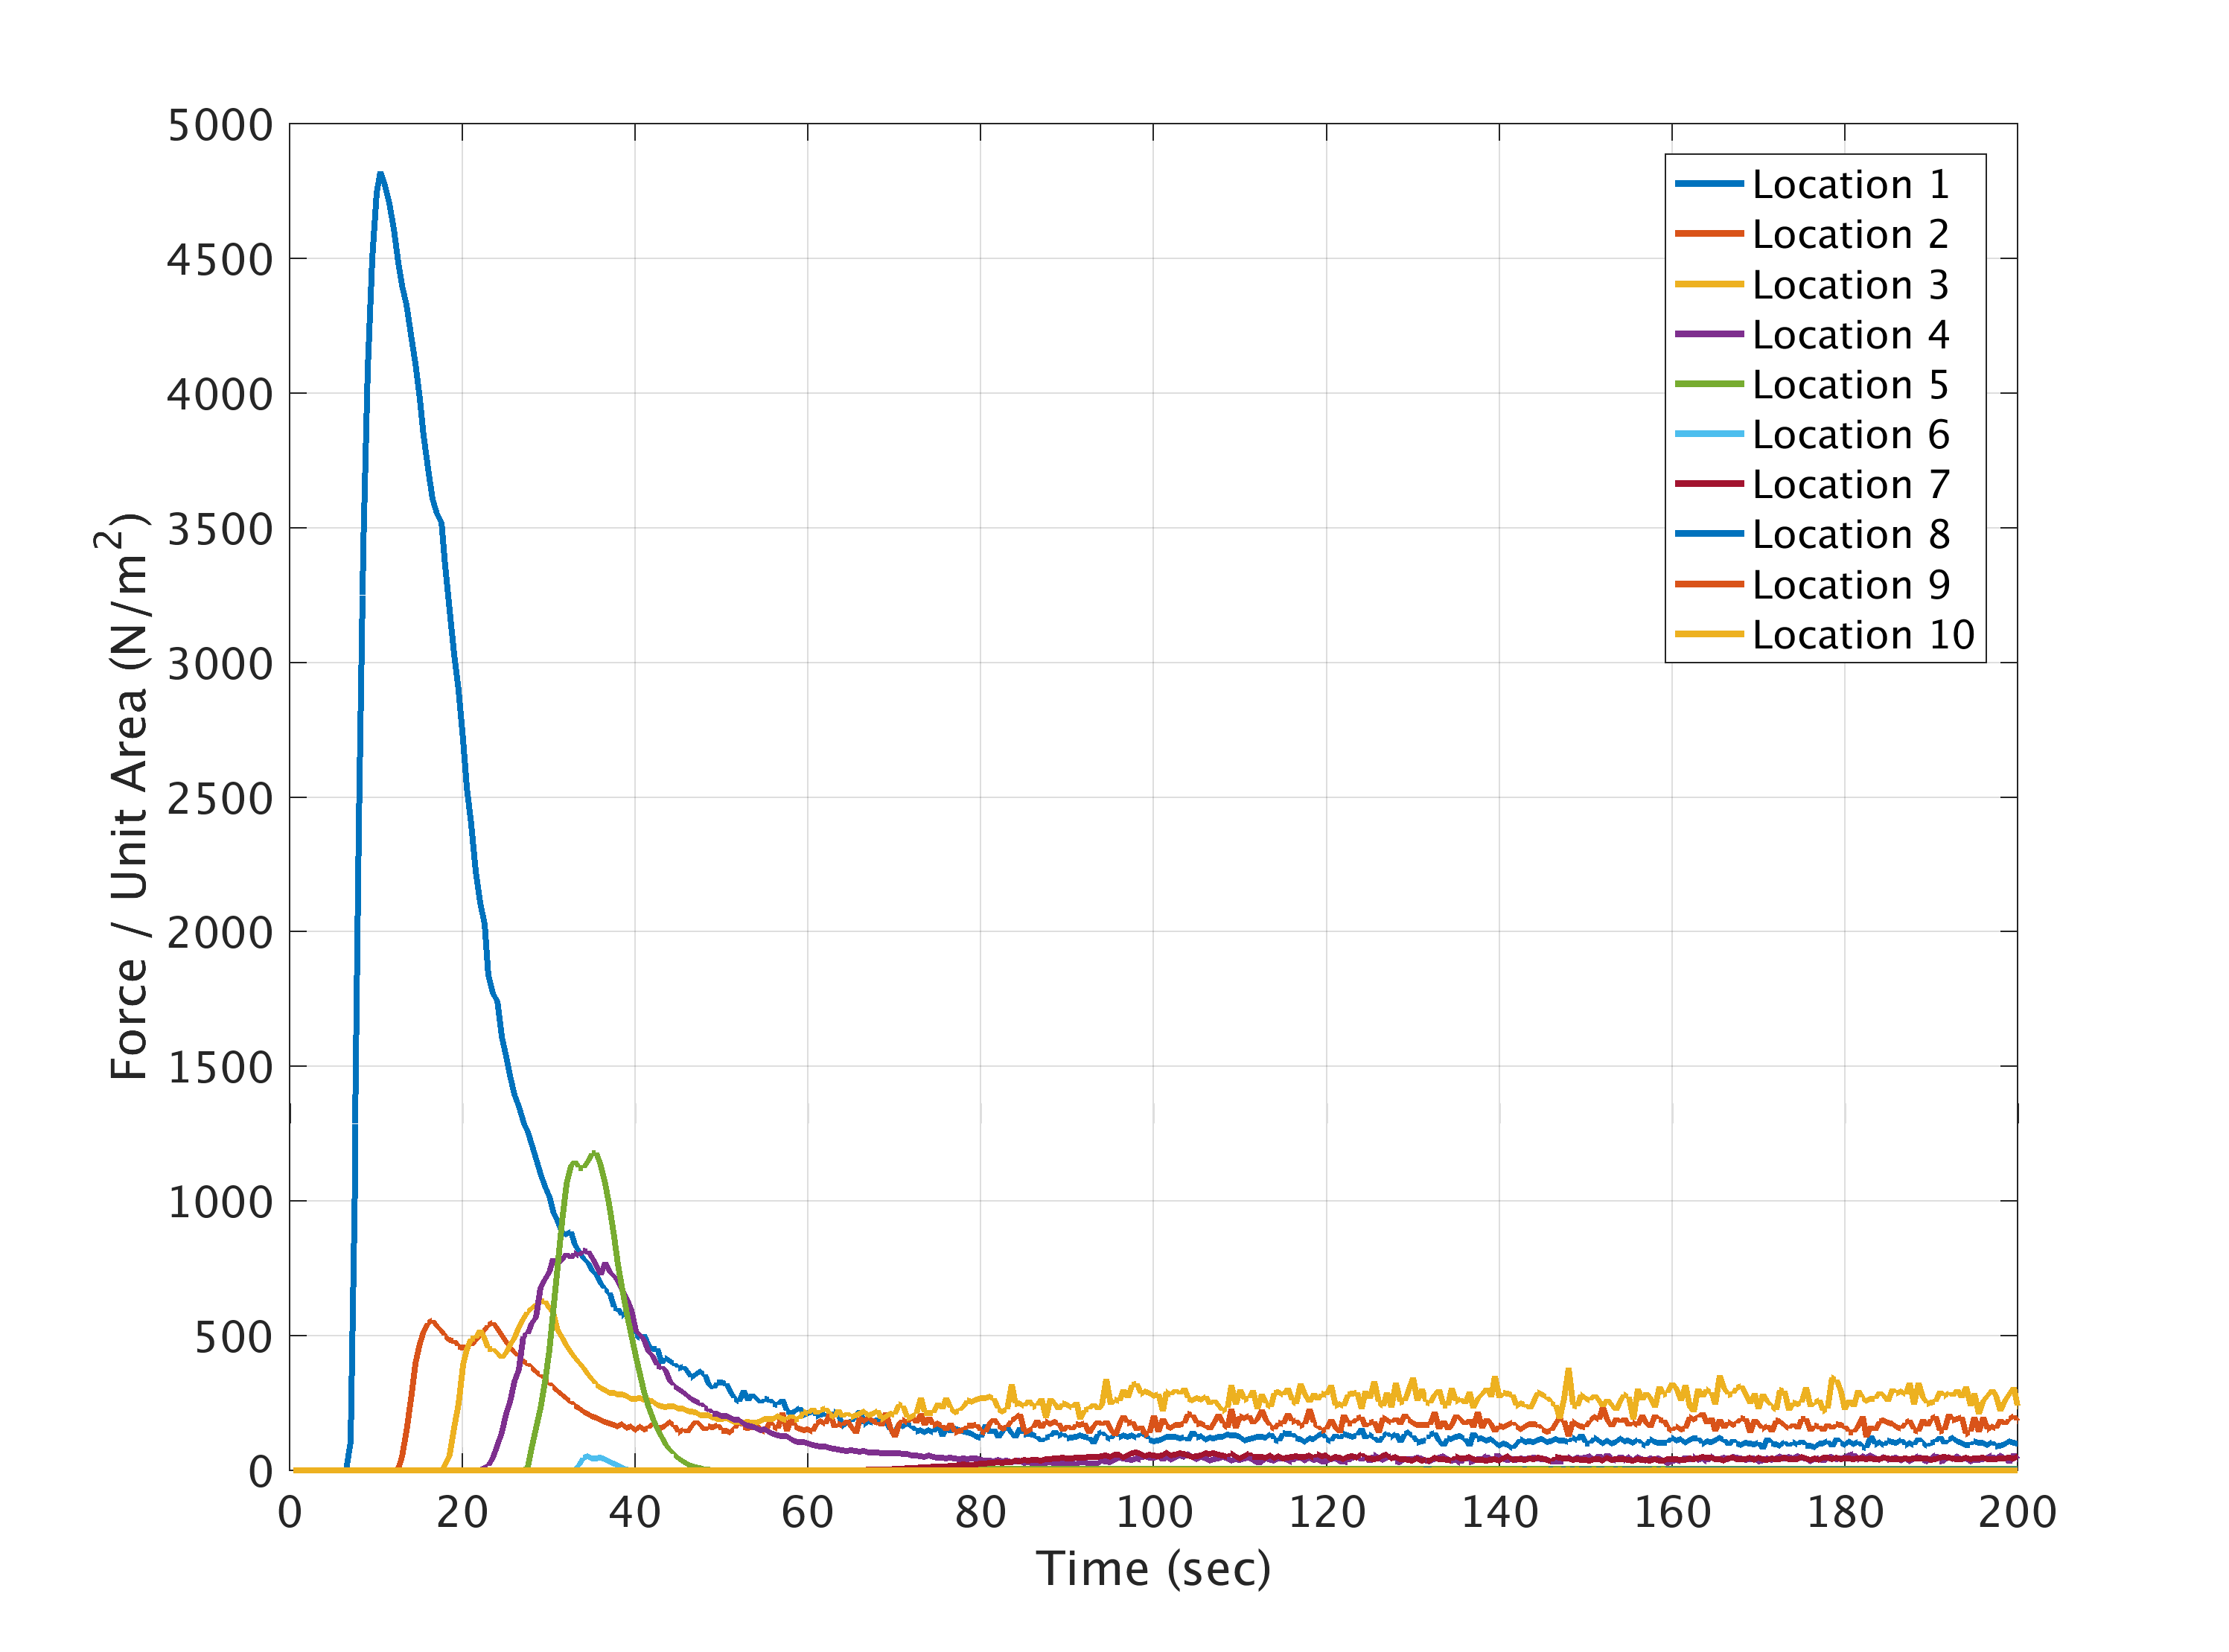
\includegraphics[width=1\textwidth]{MeansAll/FnetP_0-200.png}
        \subcaption{Zoomed view of Fig. (\ref{fig:M_FnP}).}
        \label{fig:M_FnPz}
	\end{minipage}

	\begin{minipage}[b]{0.5\linewidth}
	\centering
    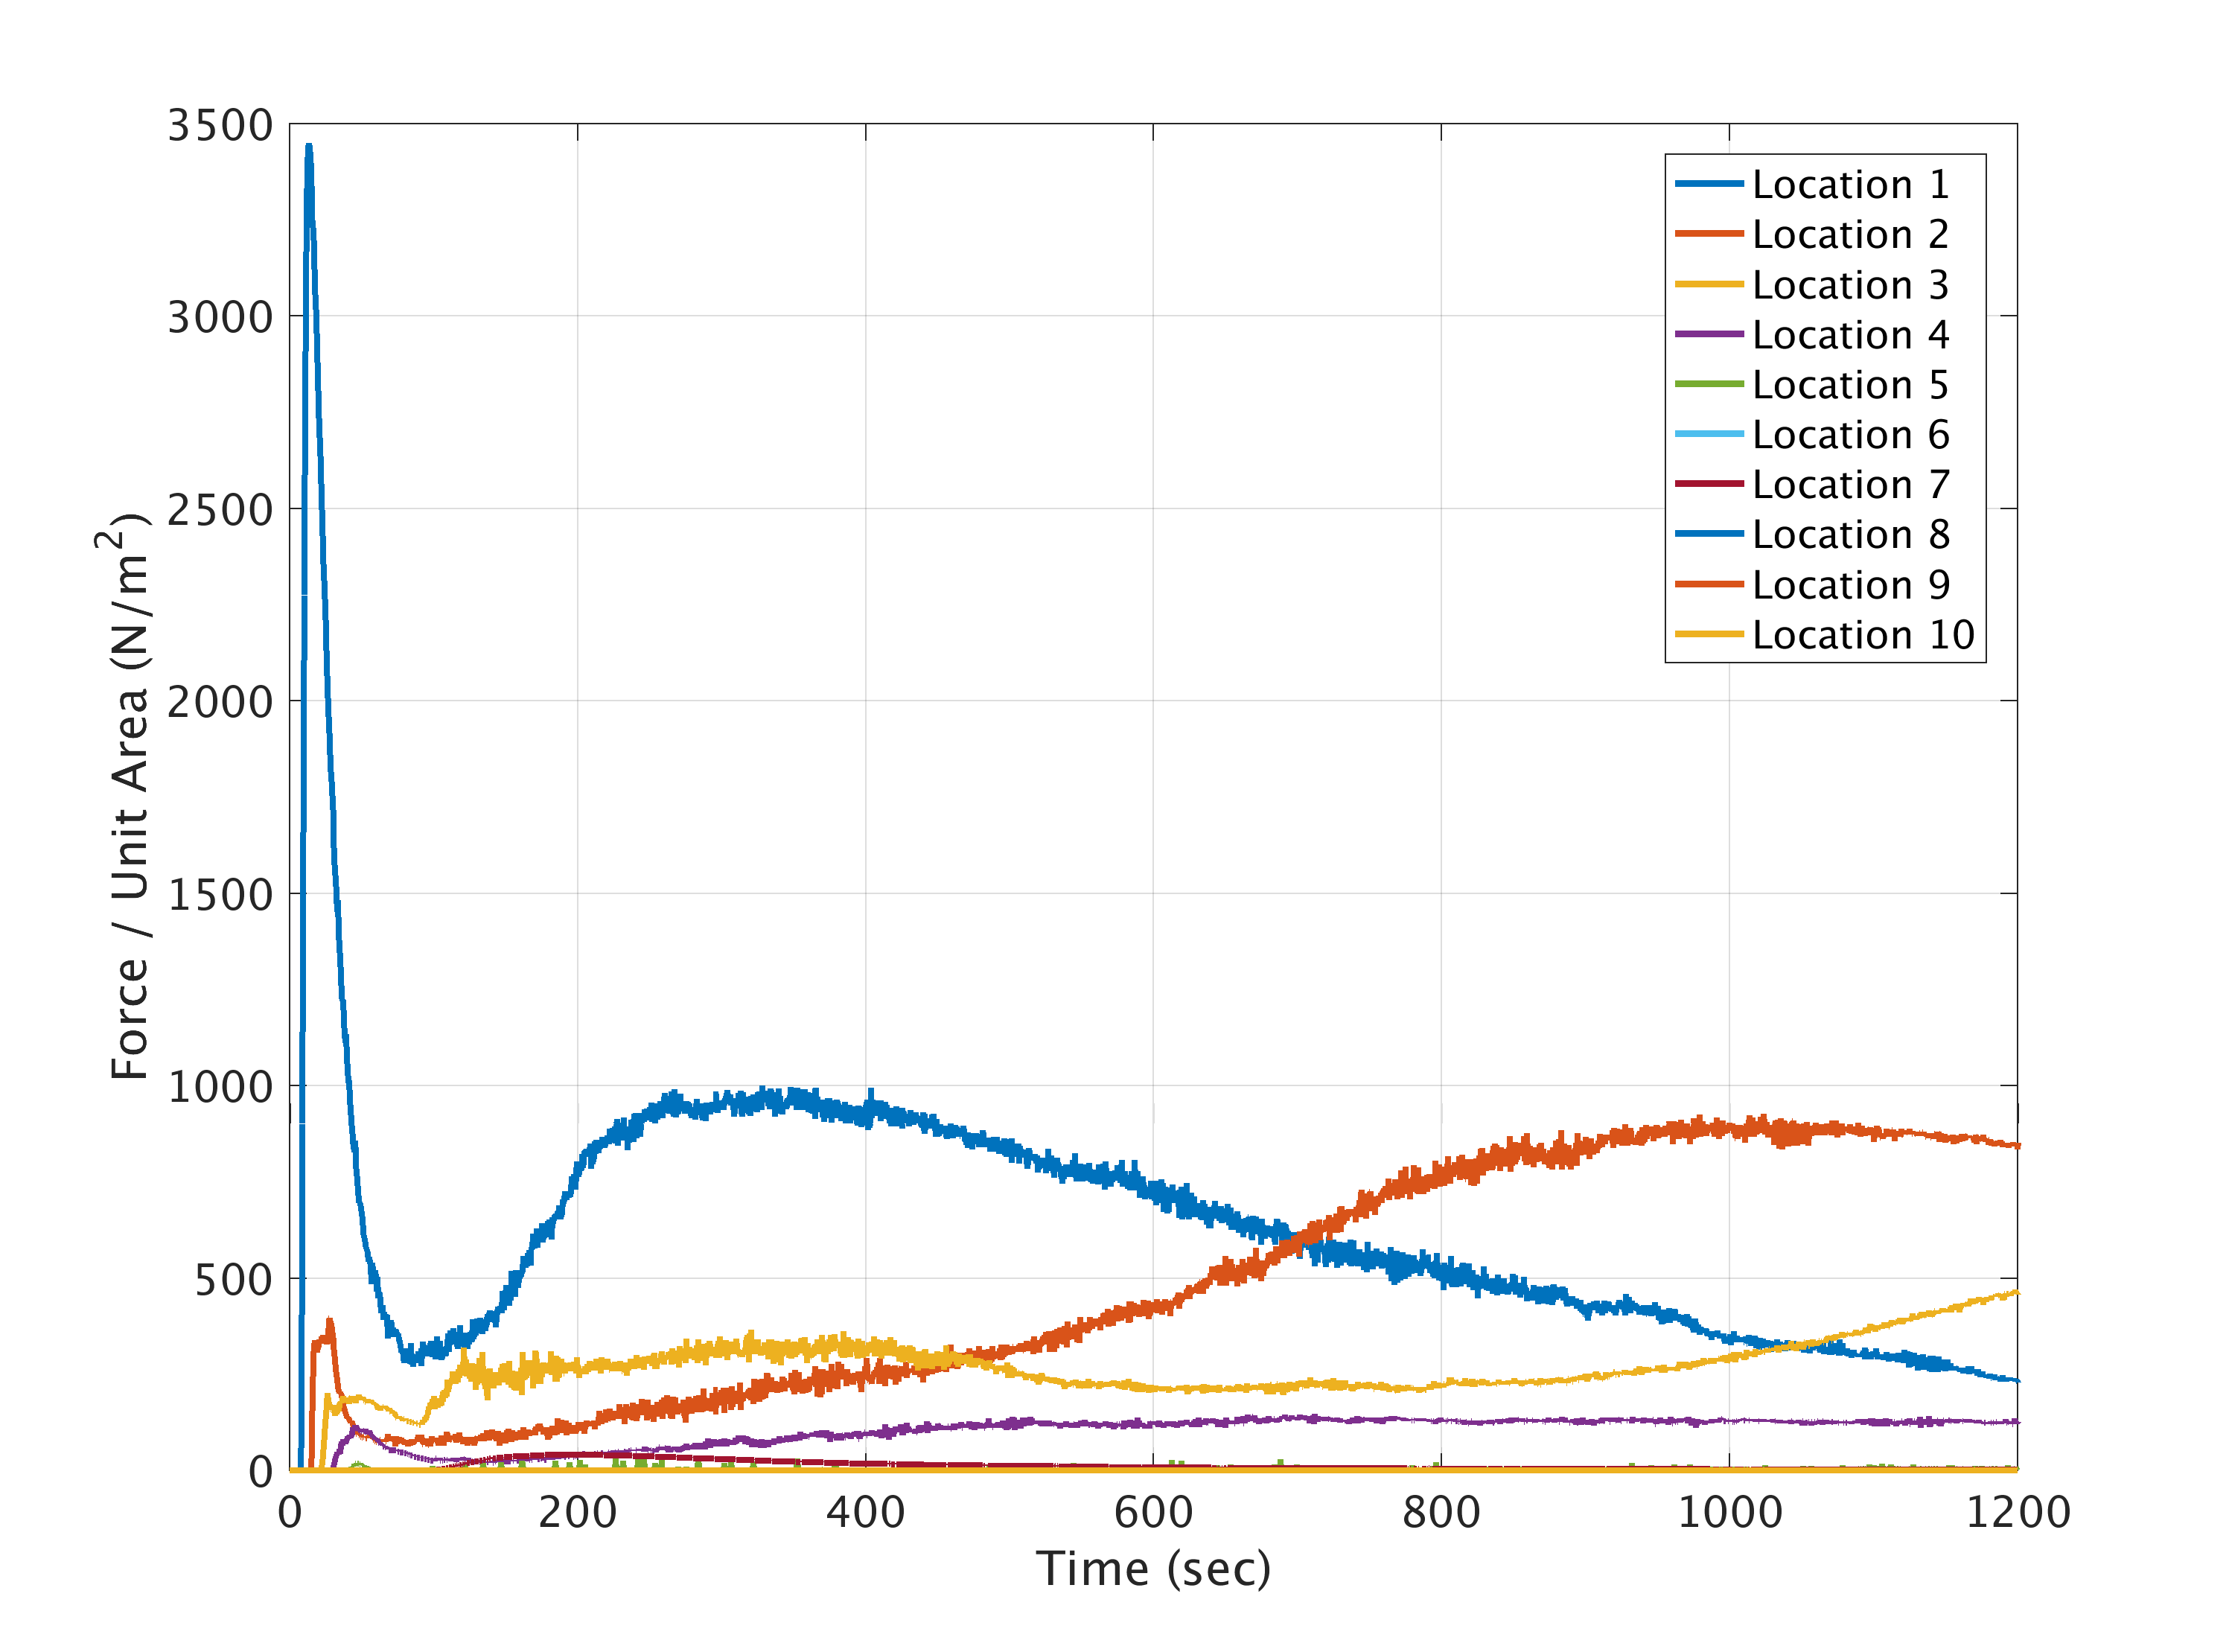
\includegraphics[width=1\textwidth]{MeansAll/FnetV.png}
        \subcaption{Net Force Records, Voellmy-Salm.}
        \label{fig:M_FnV}
	\end{minipage}
	\begin{minipage}[b]{0.5\linewidth}
	\centering
    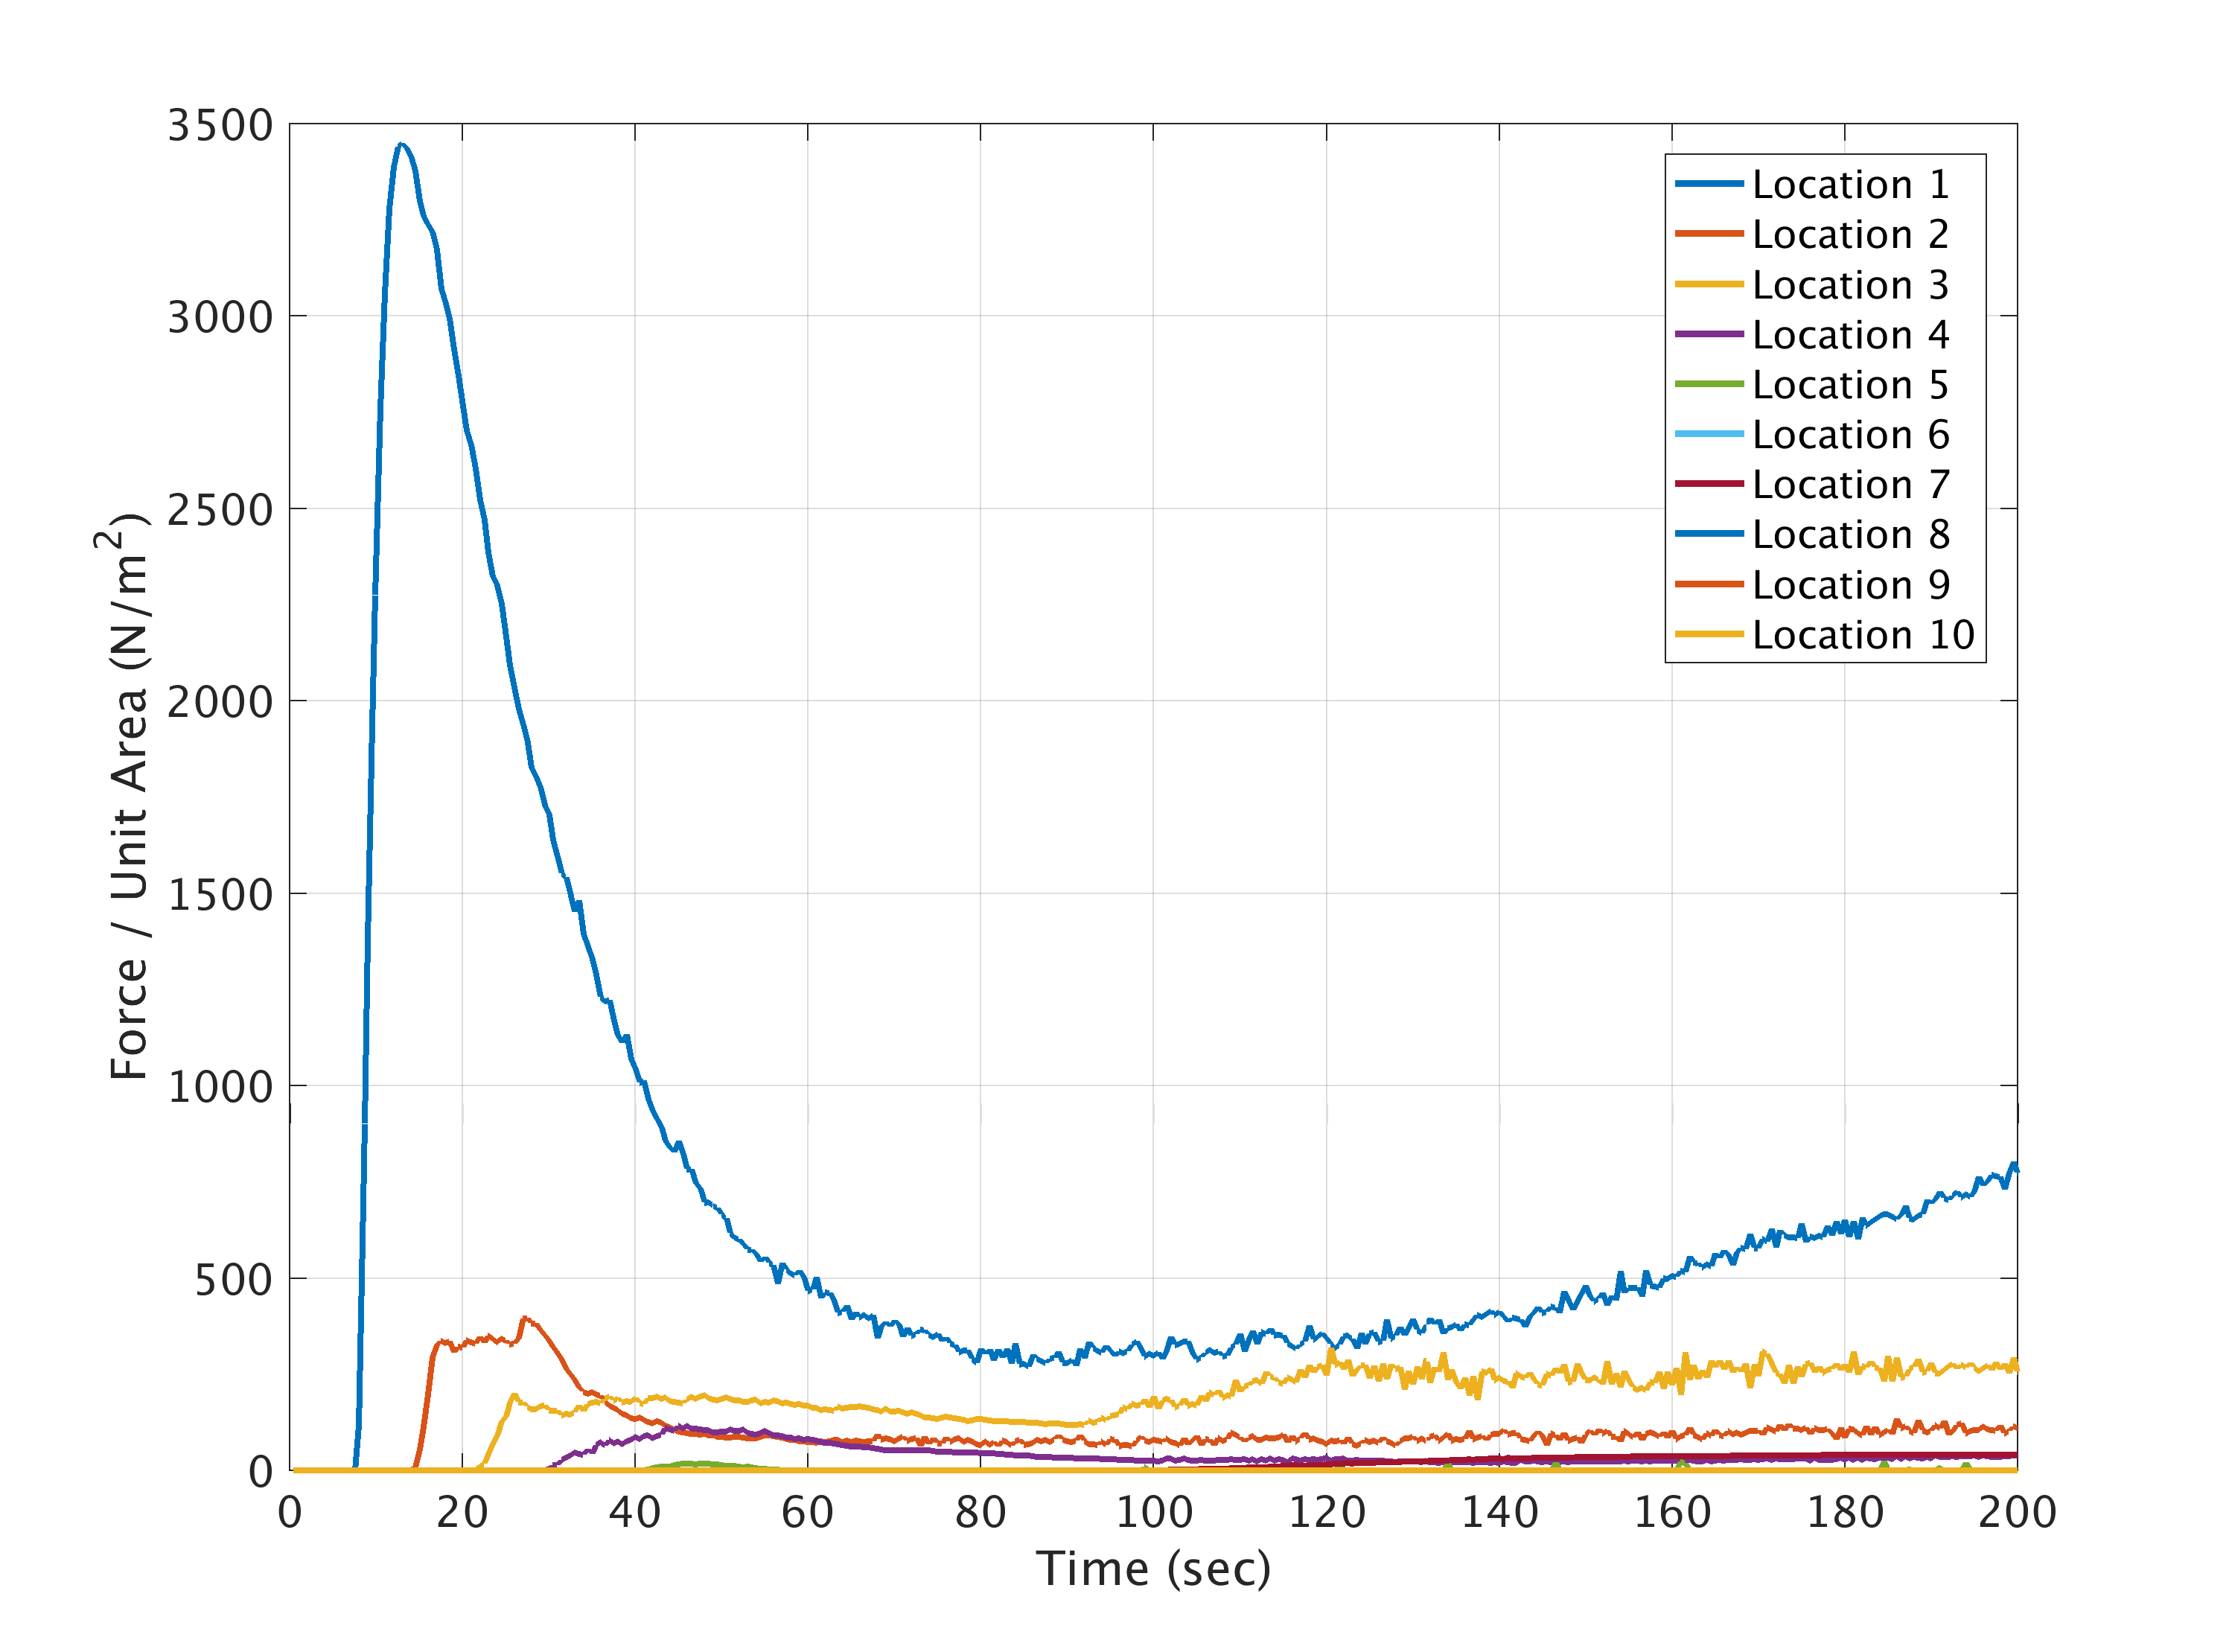
\includegraphics[width=1\textwidth]{MeansAll/FnetV_0-200.png}
        \subcaption{Zoomed view of Fig. (\ref{fig:M_FnV}).}
        \label{fig:M_FnVz}
	\end{minipage}

	\caption{Mean Values of net force records at all the specified locations.}\label{fig:M_Fnet}
\end{figure}
\newpage
Looking at Figures \ref{fig:M_VCall}, \ref{fig:M_VPall} and \ref{fig:M_VVall}, we can see a recocnizable ascending-descending behavior, $\nearrow \ \searrow$, in mean values of velocity records for Mohr-Coulomb model and the peak value is happening at $4^{\mathrm{th}}$ location. In Pouliquen-Forterre model we can also see an ascending-descending behavior, however, the peak value occurs at $2^{\mathrm{nd}}$ location. Interestingly, we only see a descending behavior, $\searrow$, in Voellmy-Salm model simulations. Furthermore, the average values of peak velocity record is higher for Mohr-Coulomb model ($\sim$45 m/s) than Pouliquen-Forterre velocity peak ($\sim$30 m/s) and Voellmy-Salm velocity peak ($\sim$15 m/s).

\begin{figure}[H]

	\begin{minipage}[b]{0.5\linewidth}
	\centering
    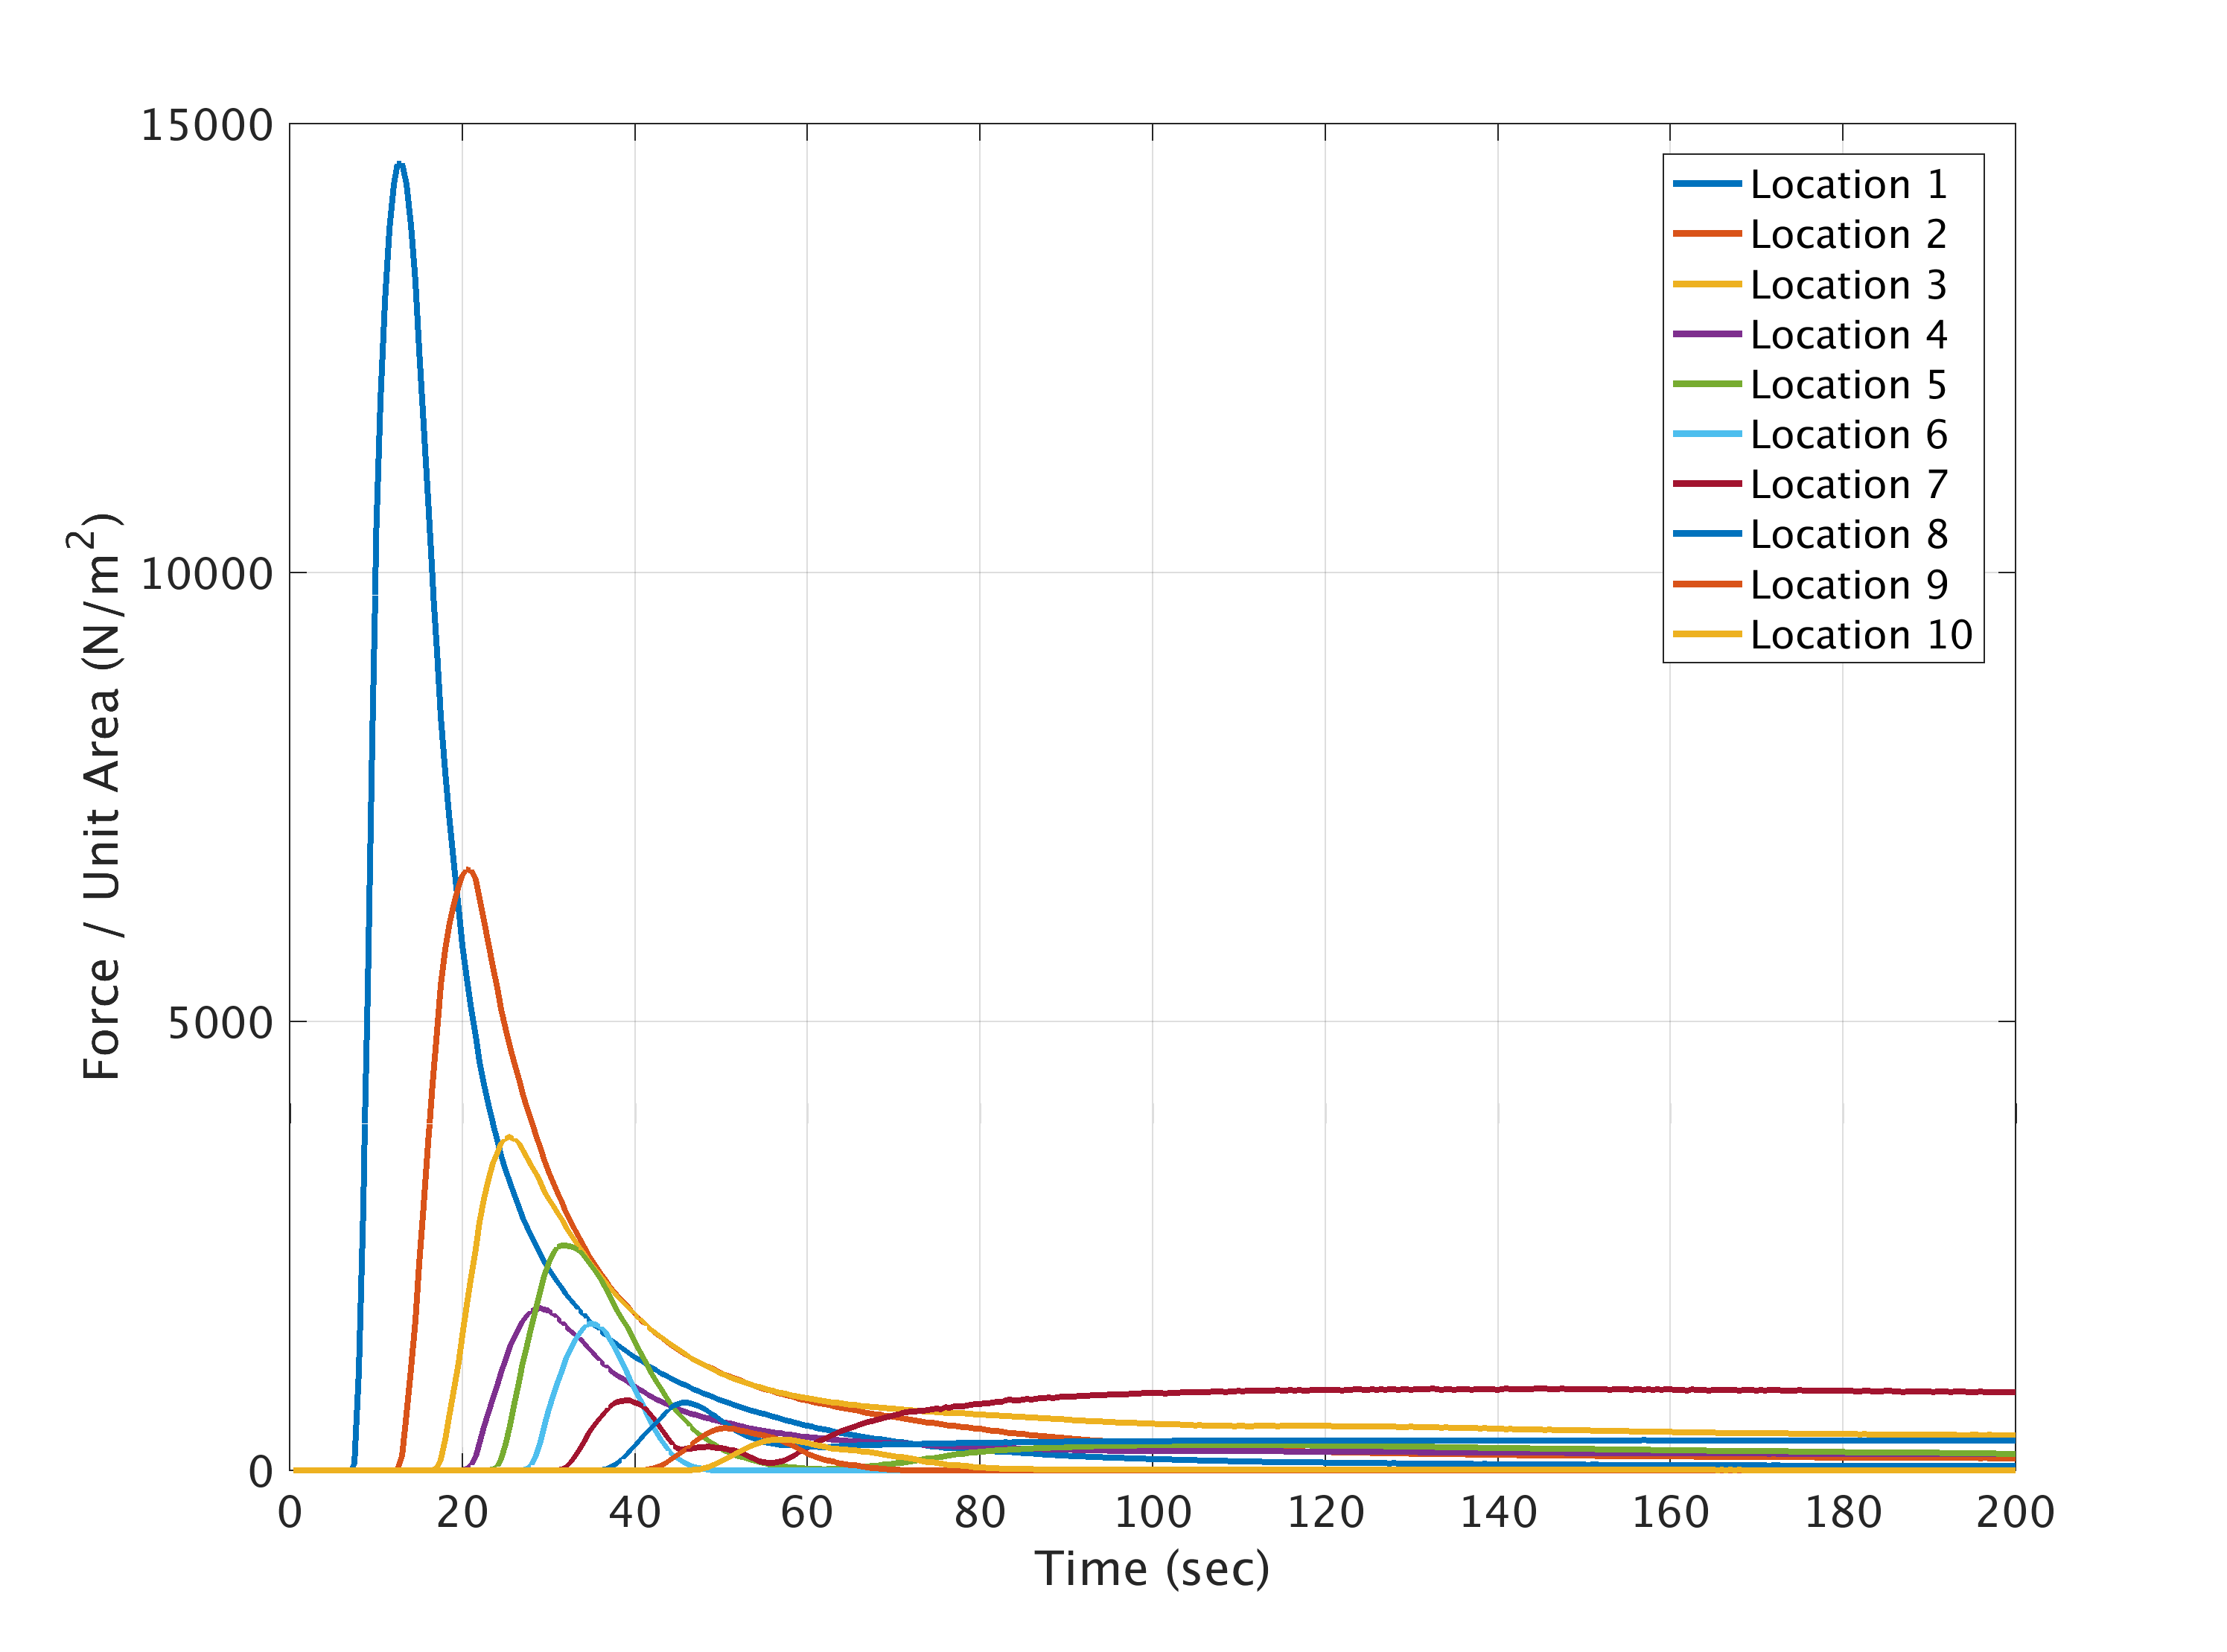
\includegraphics[width=1\textwidth]{MeansAll/FgravC_all.png}     
        \subcaption{Gravitational Force Records, Mohr-Coulomb.}
        \label{fig:M_FgCall}
	\end{minipage}
	\begin{minipage}[b]{0.5\linewidth}
	\centering
    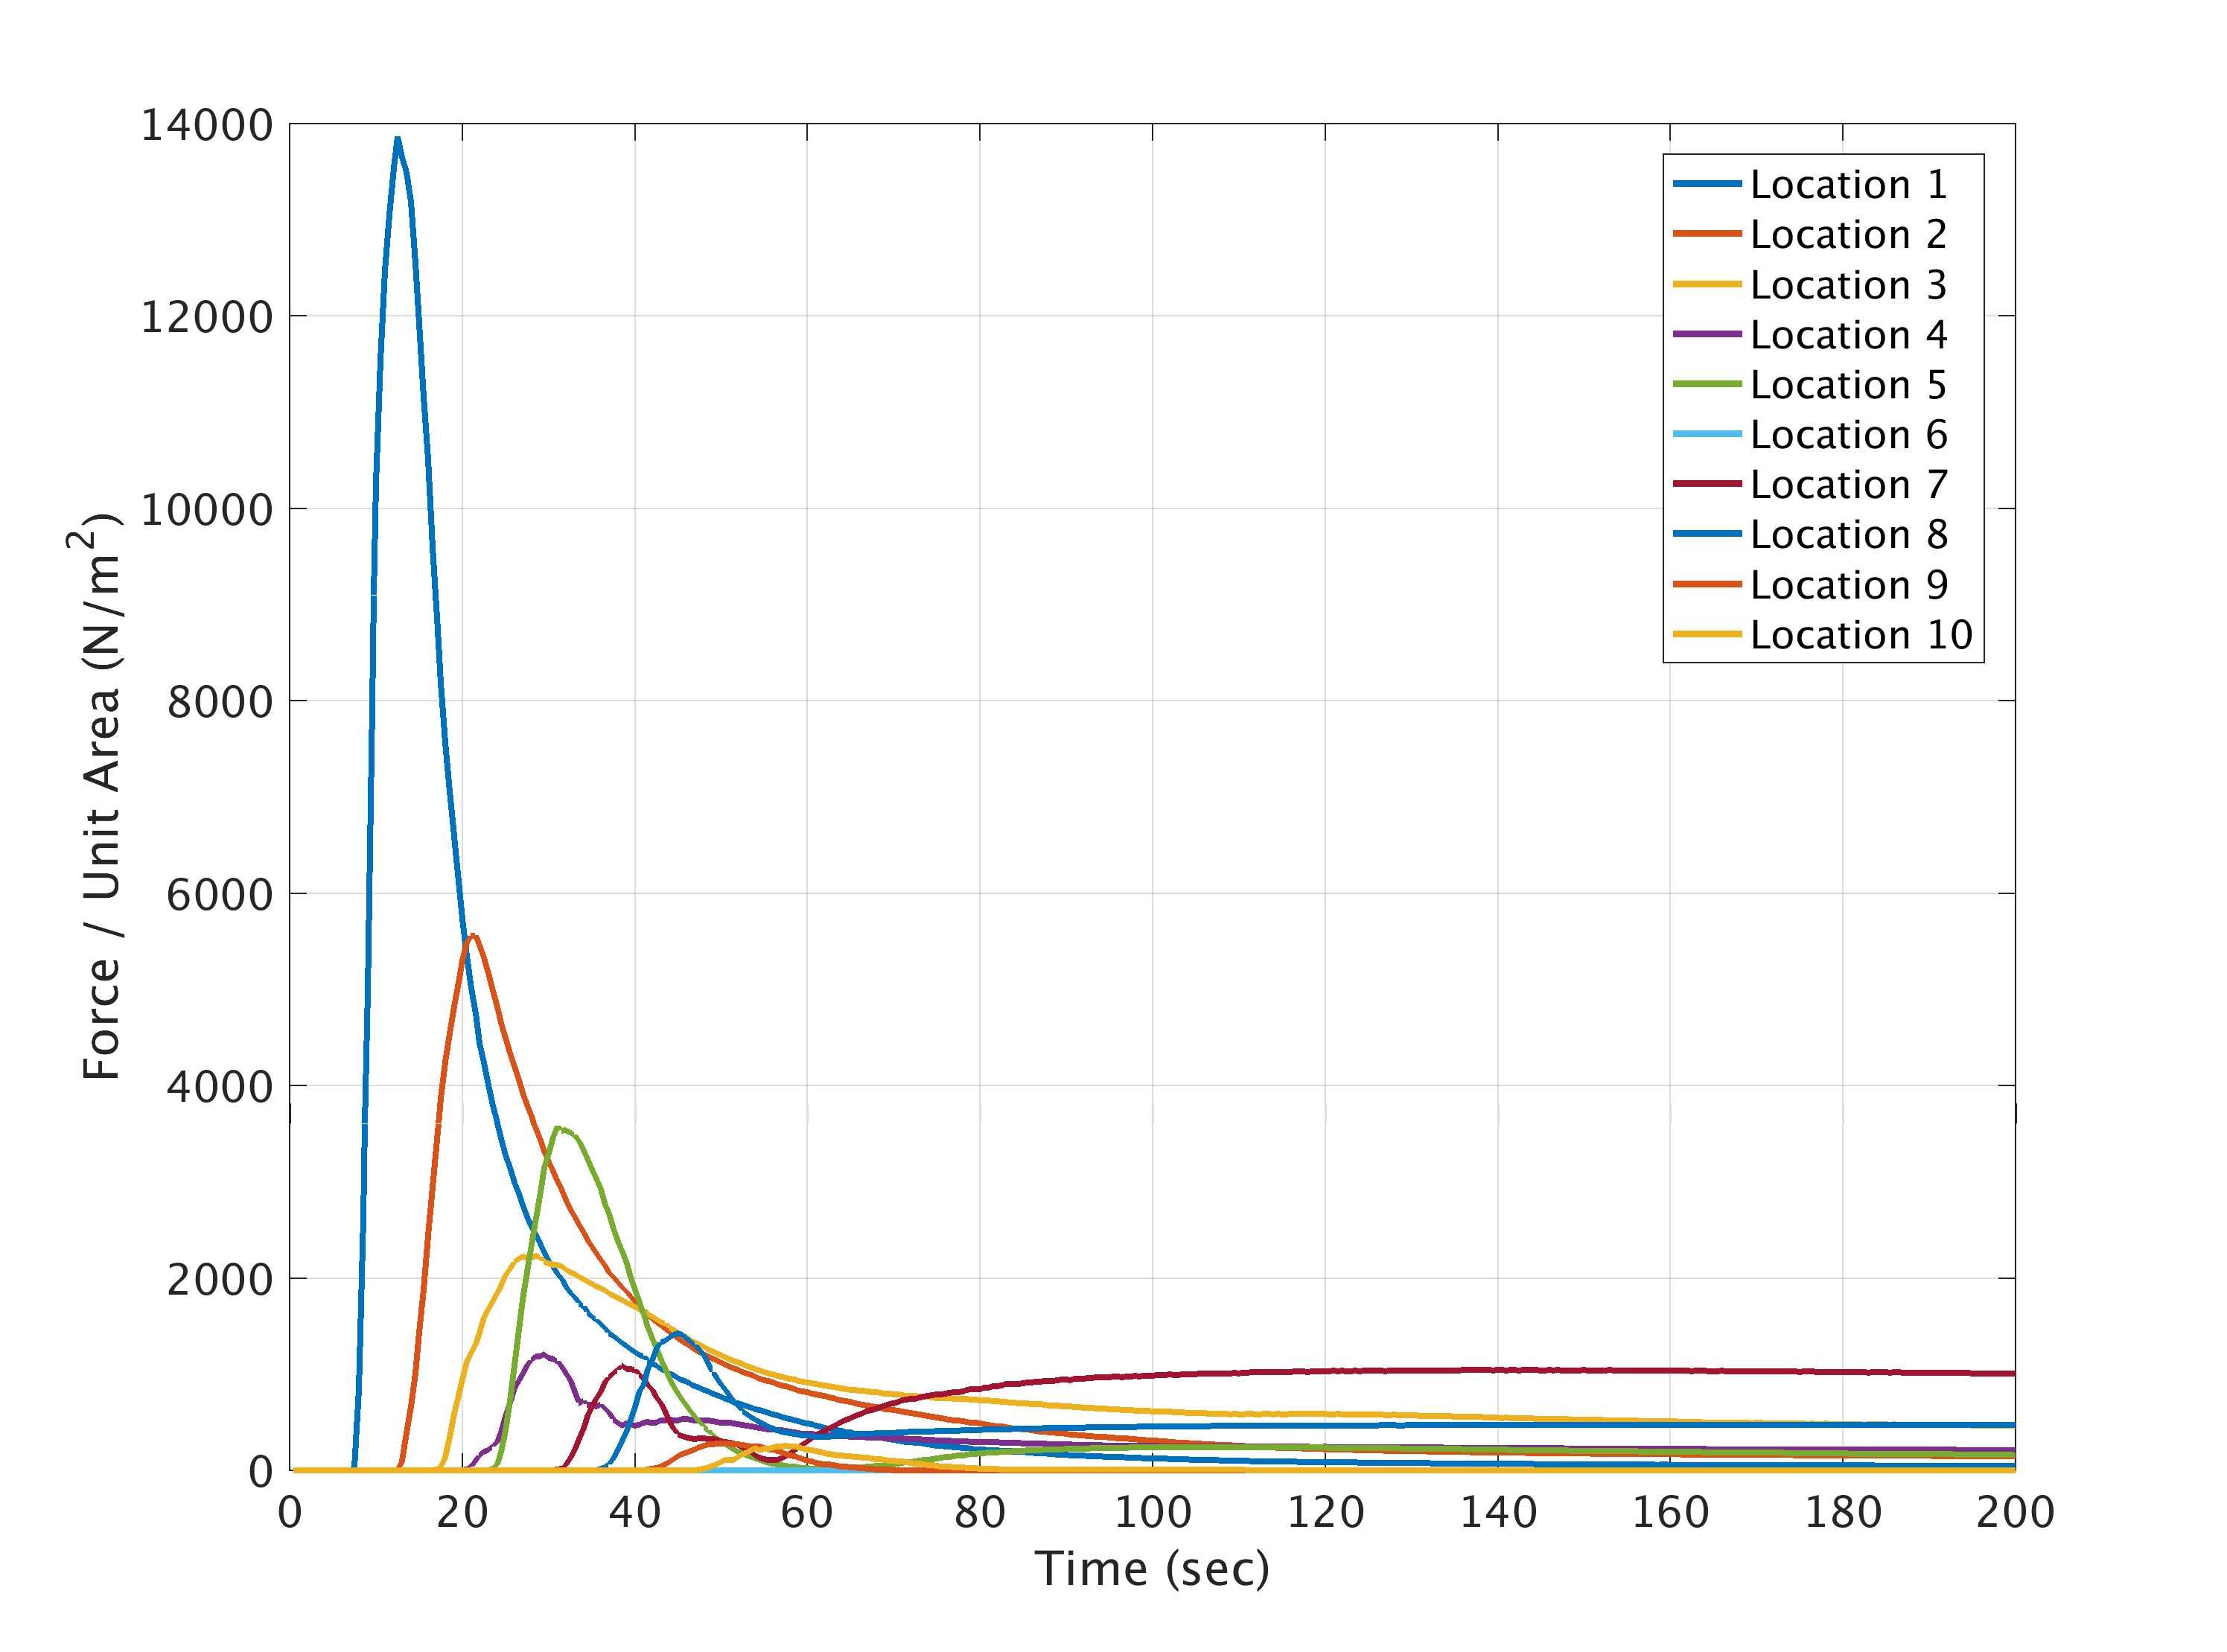
\includegraphics[width=1\textwidth]{MeansAll/FbedC_all.png}     
        \subcaption{Bed Resisting Force Records, Mohr-Coulomb.}
        \label{fig:M_FbCall}
	\end{minipage}
	
	\begin{minipage}[b]{0.5\linewidth}
	\centering
    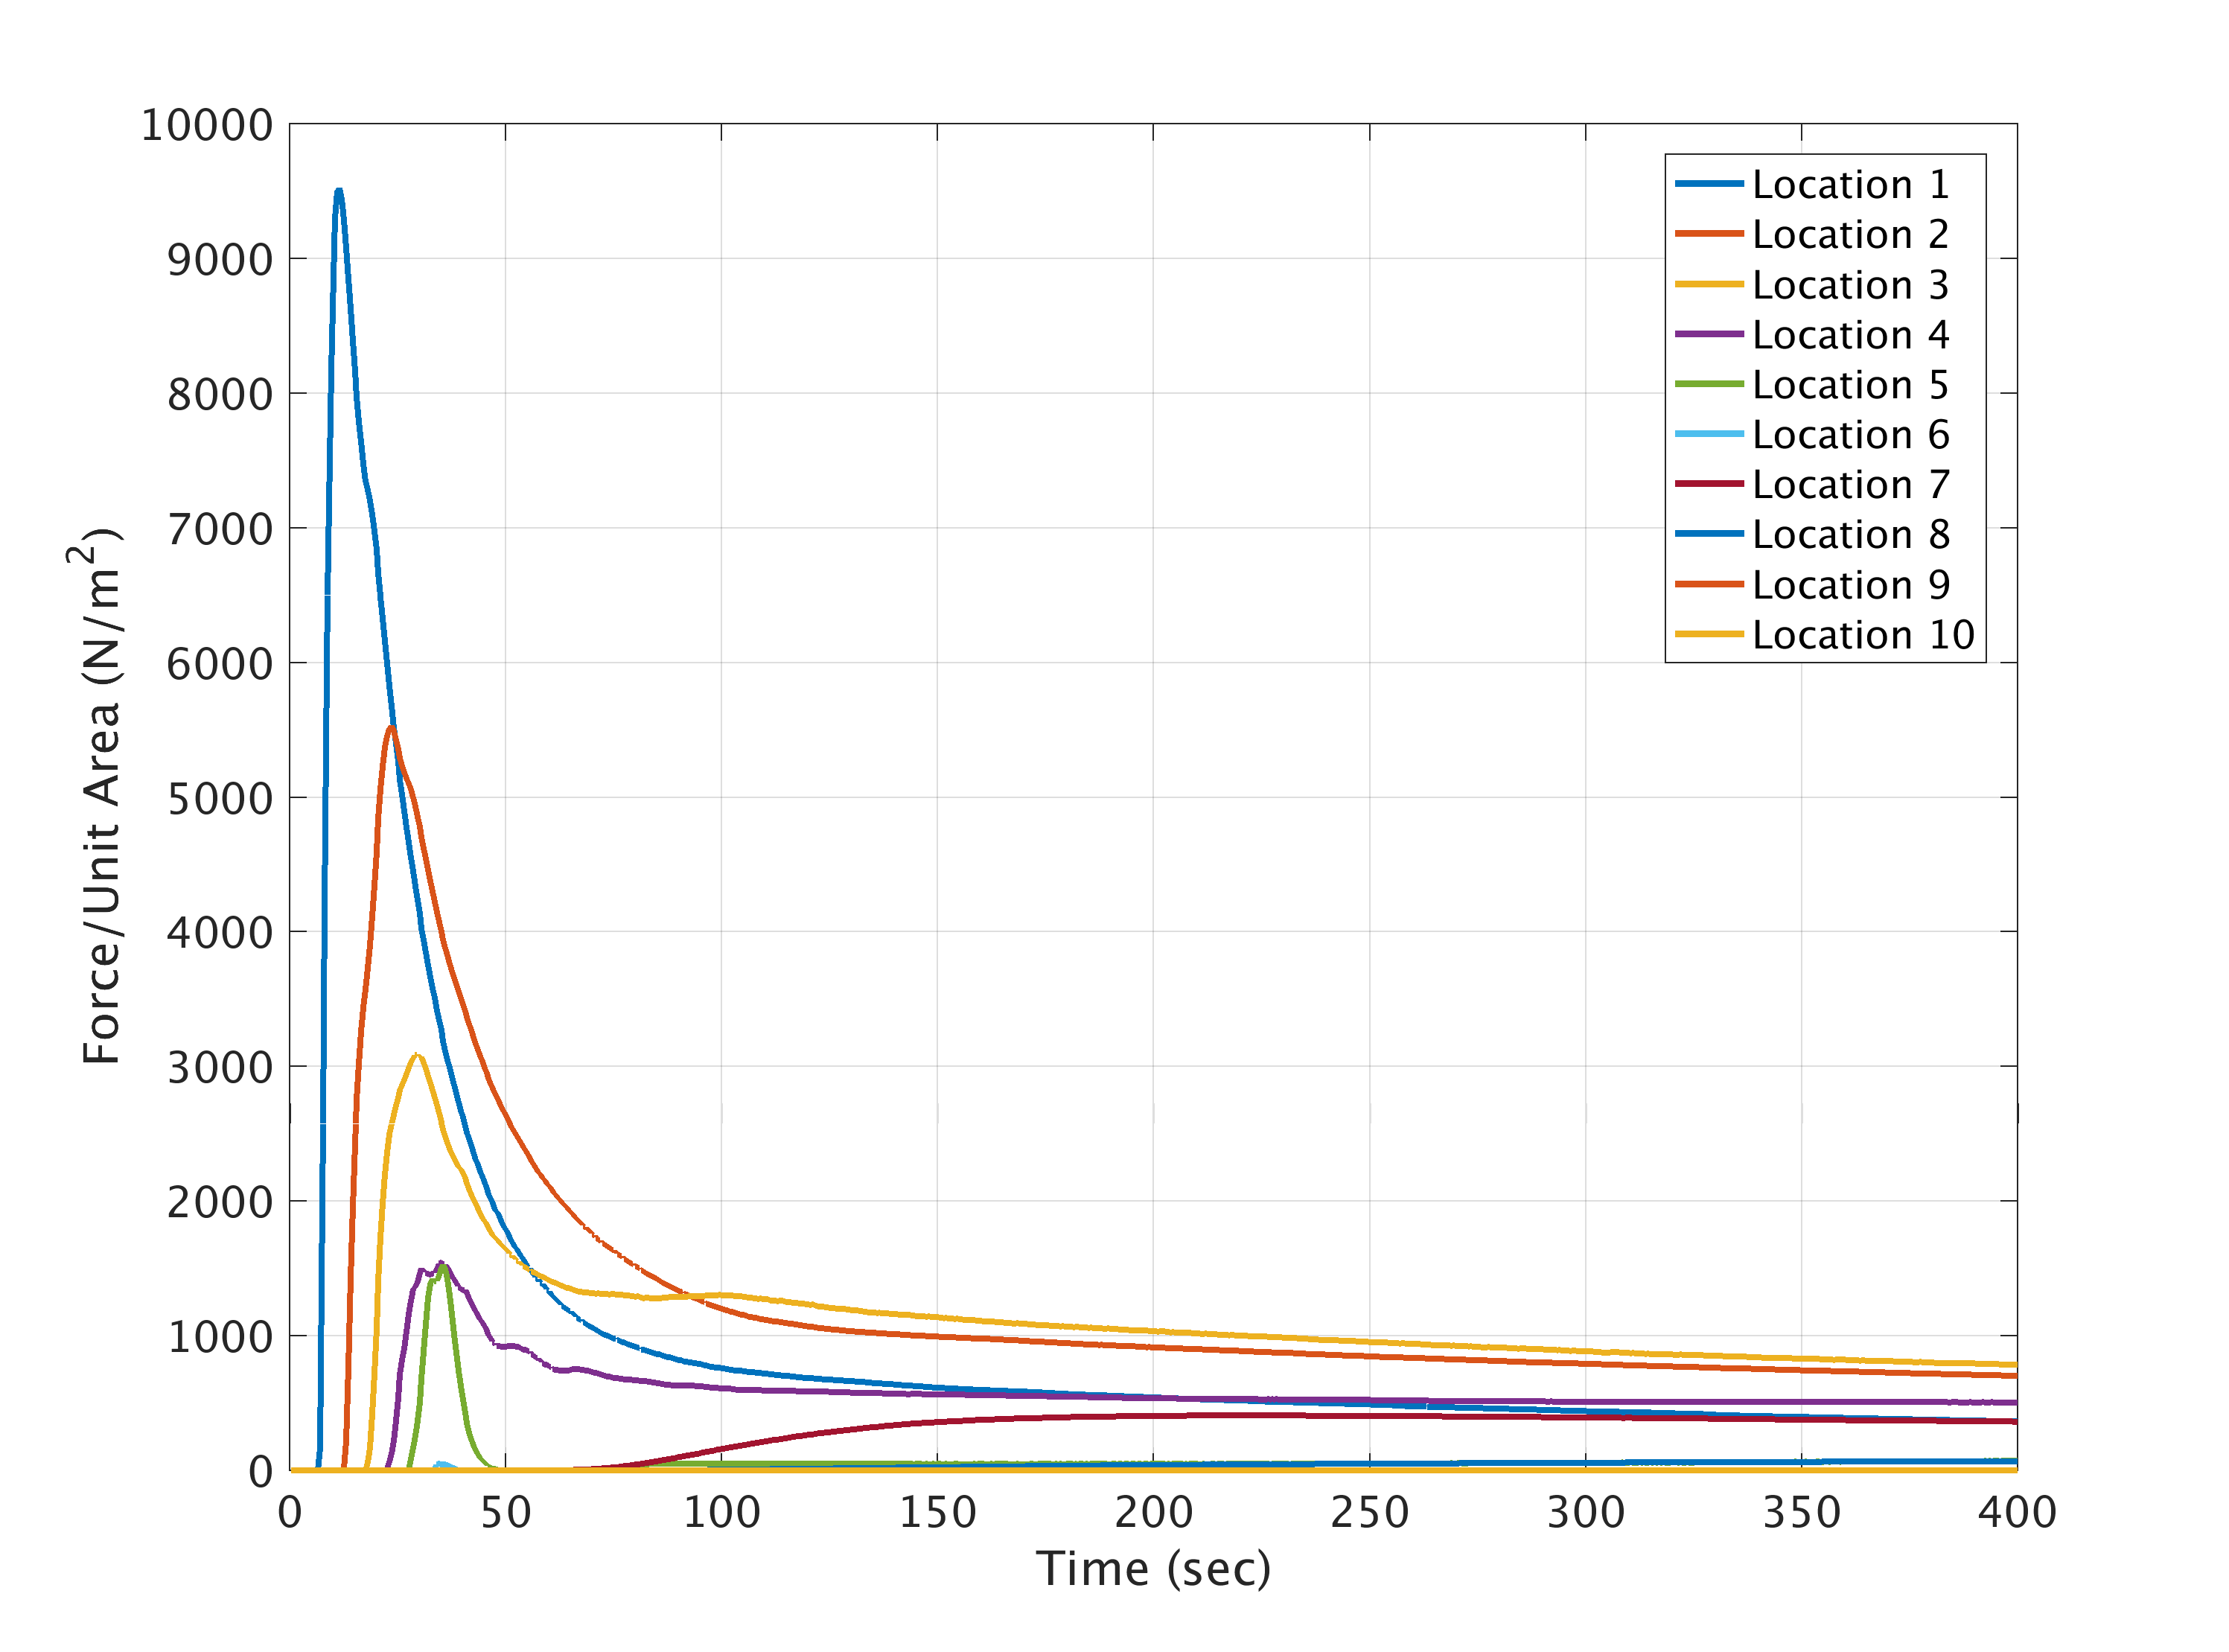
\includegraphics[width=1\textwidth]{MeansAll/FgravP_all.png}
        \subcaption{Gravitational Force Records, Pouliquen-Forterre.}
        \label{fig:M_FgPall}
	\end{minipage}	
	\begin{minipage}[b]{0.5\linewidth}
	\centering
    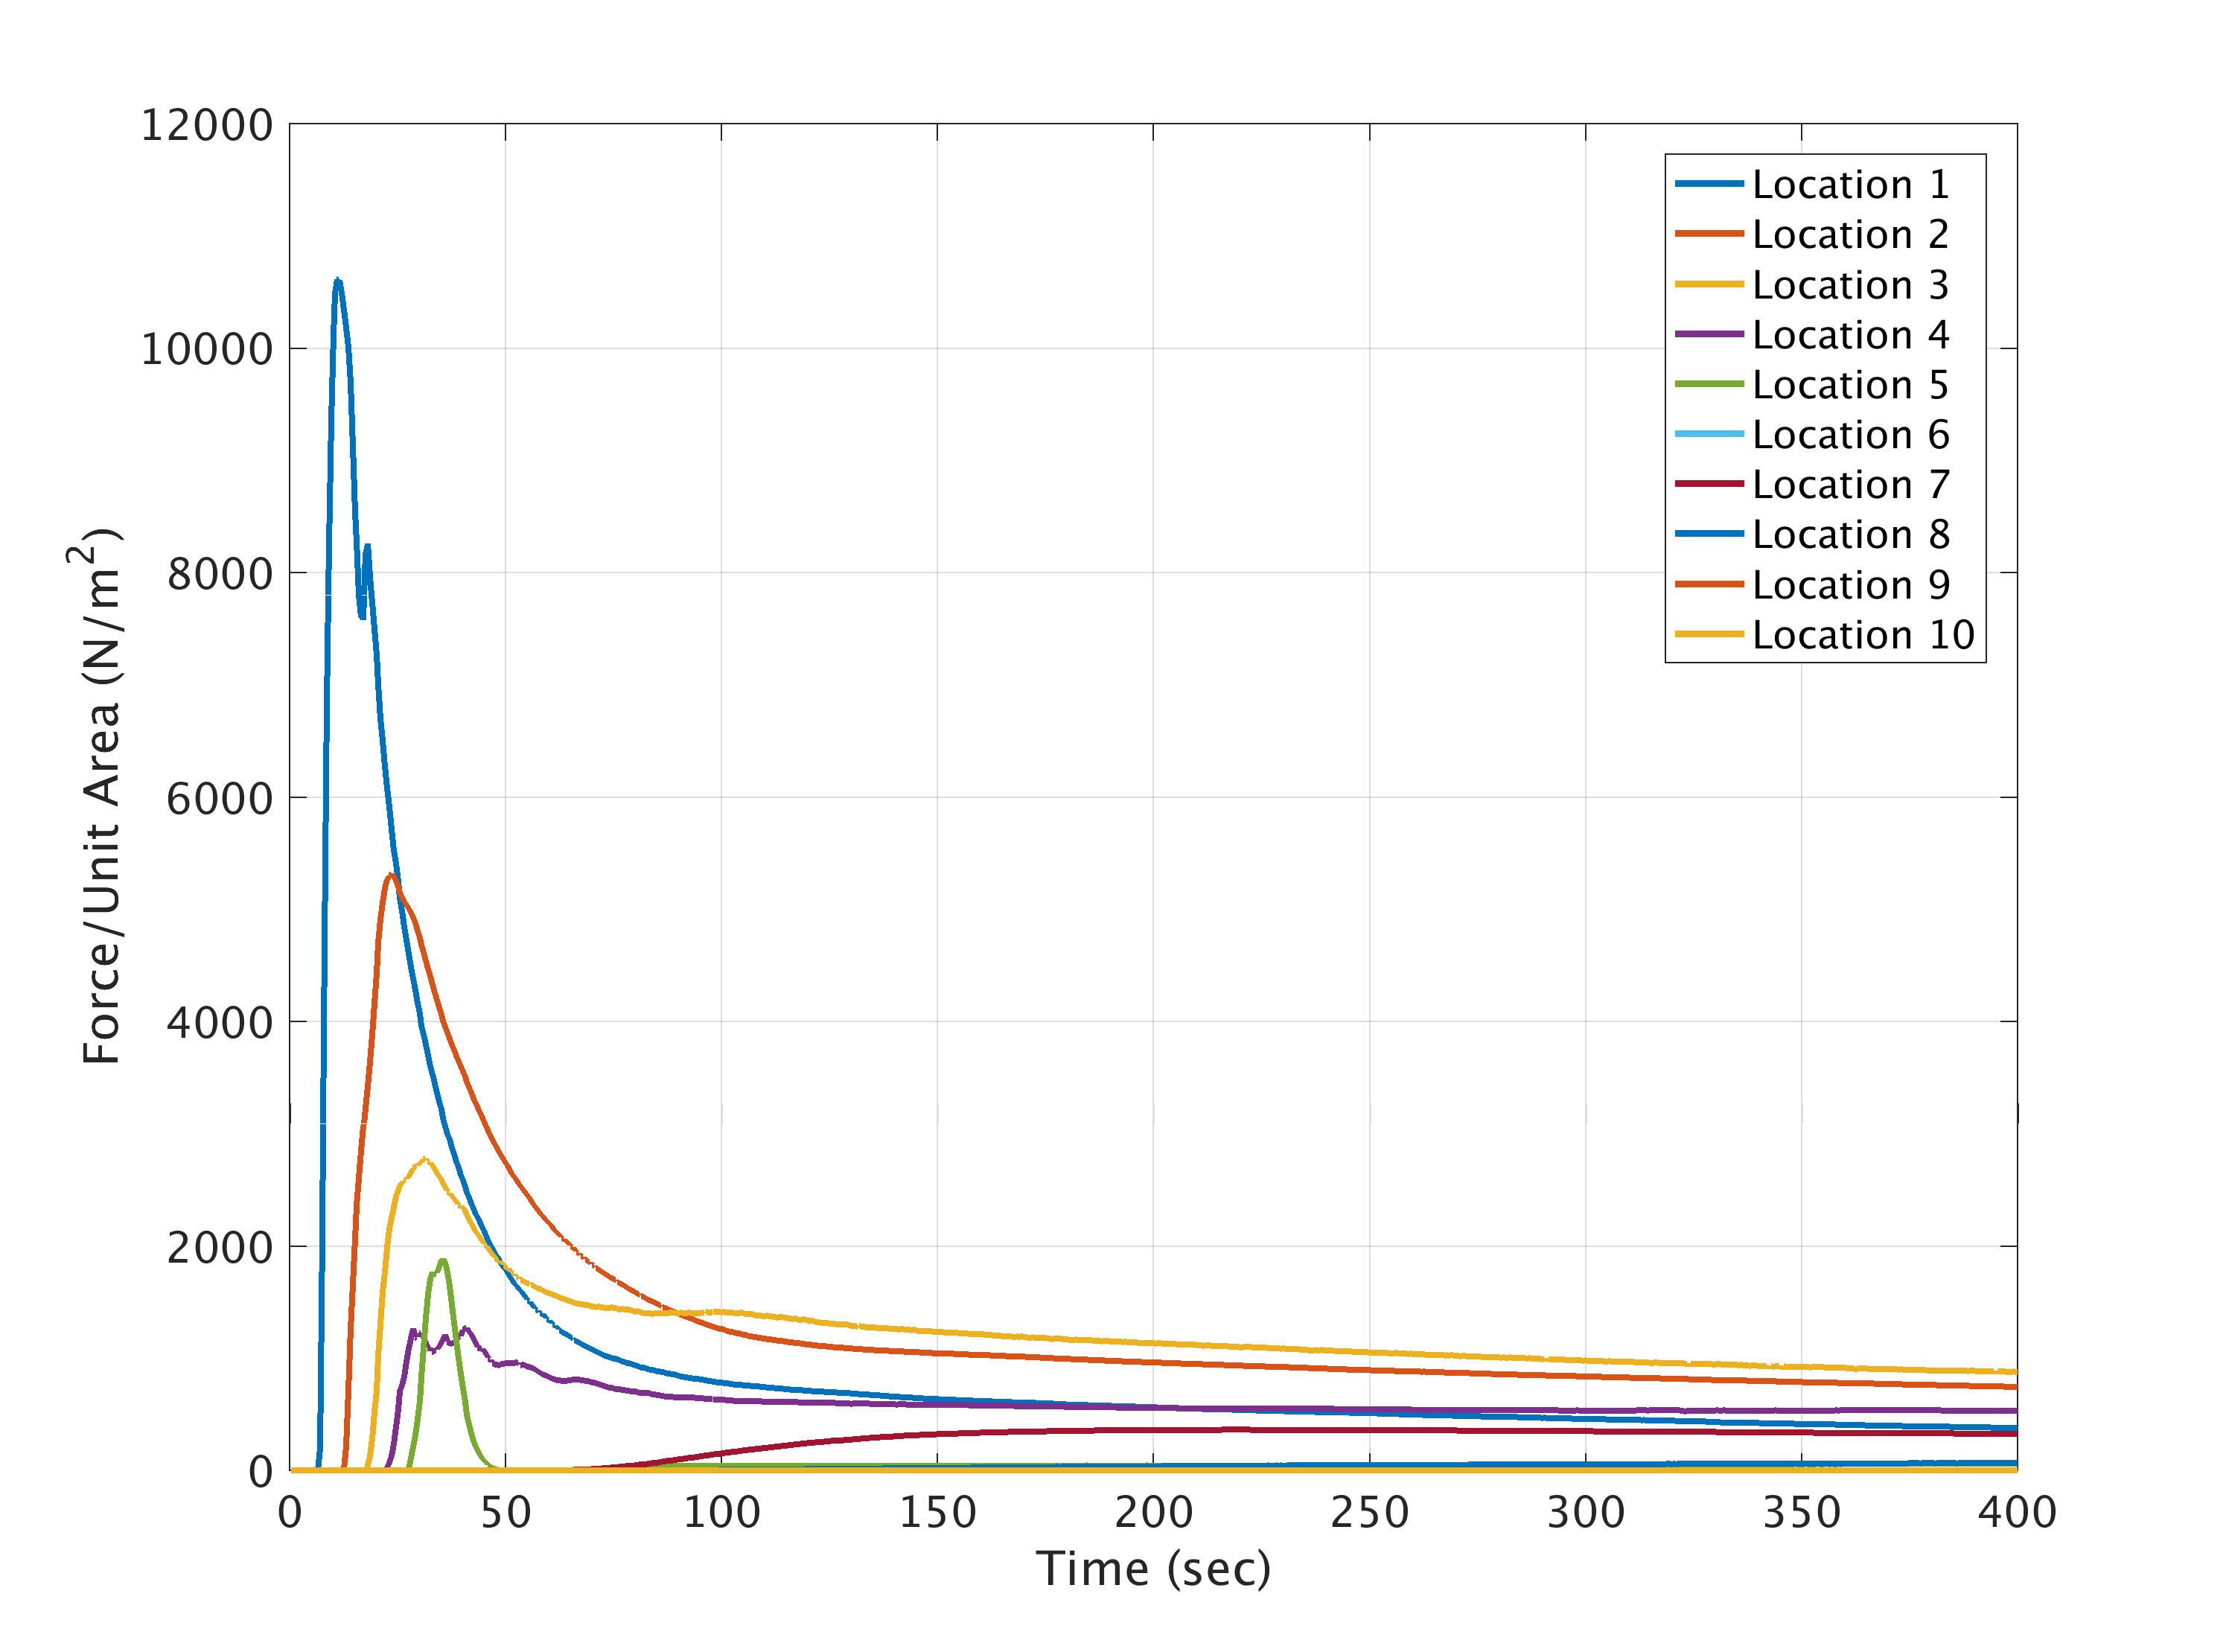
\includegraphics[width=1\textwidth]{MeansAll/FbedP_all.png}
        \subcaption{Bed Resisting Force Records, Pouliquen-Forterre.}
        \label{fig:M_FbPall}
	\end{minipage}

	\begin{minipage}[b]{0.5\linewidth}
	\centering
    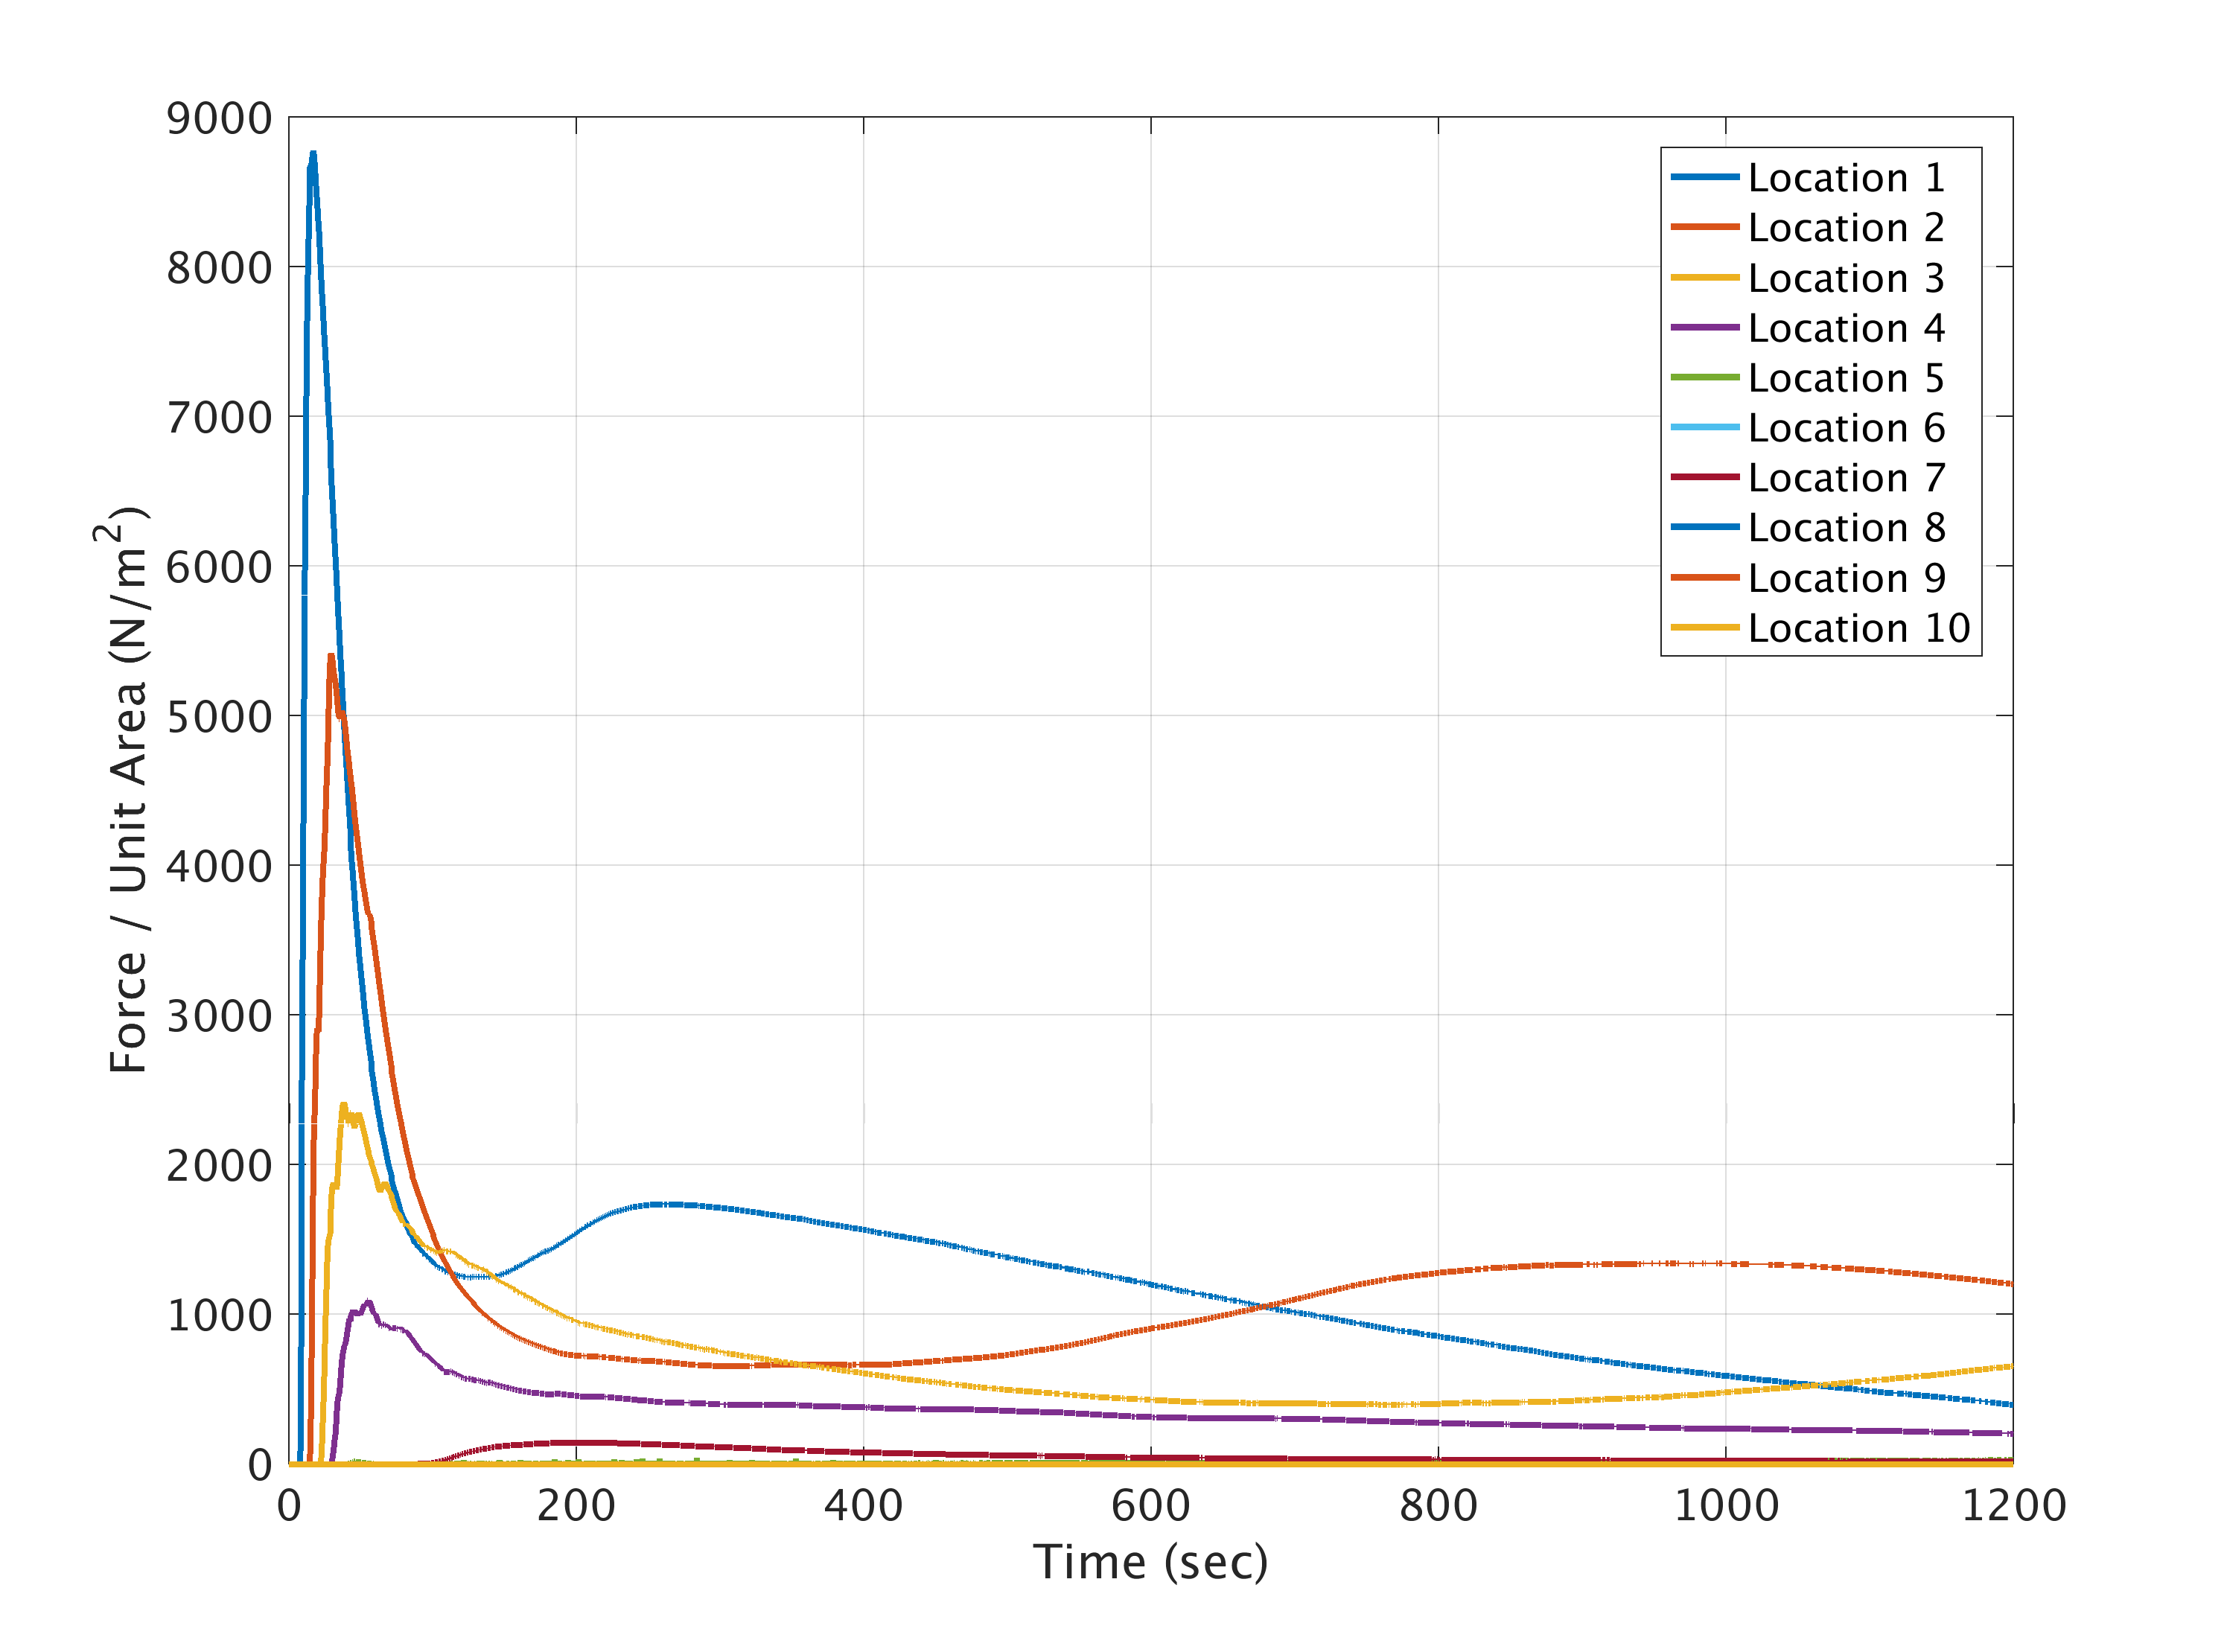
\includegraphics[width=1\textwidth]{MeansAll/FgravV_all.png}
        \subcaption{Gravitational Force Records, Voellmy-Salm.}
        \label{fig:M_FgVall}
	\end{minipage}
	\begin{minipage}[b]{0.5\linewidth}
	\centering
    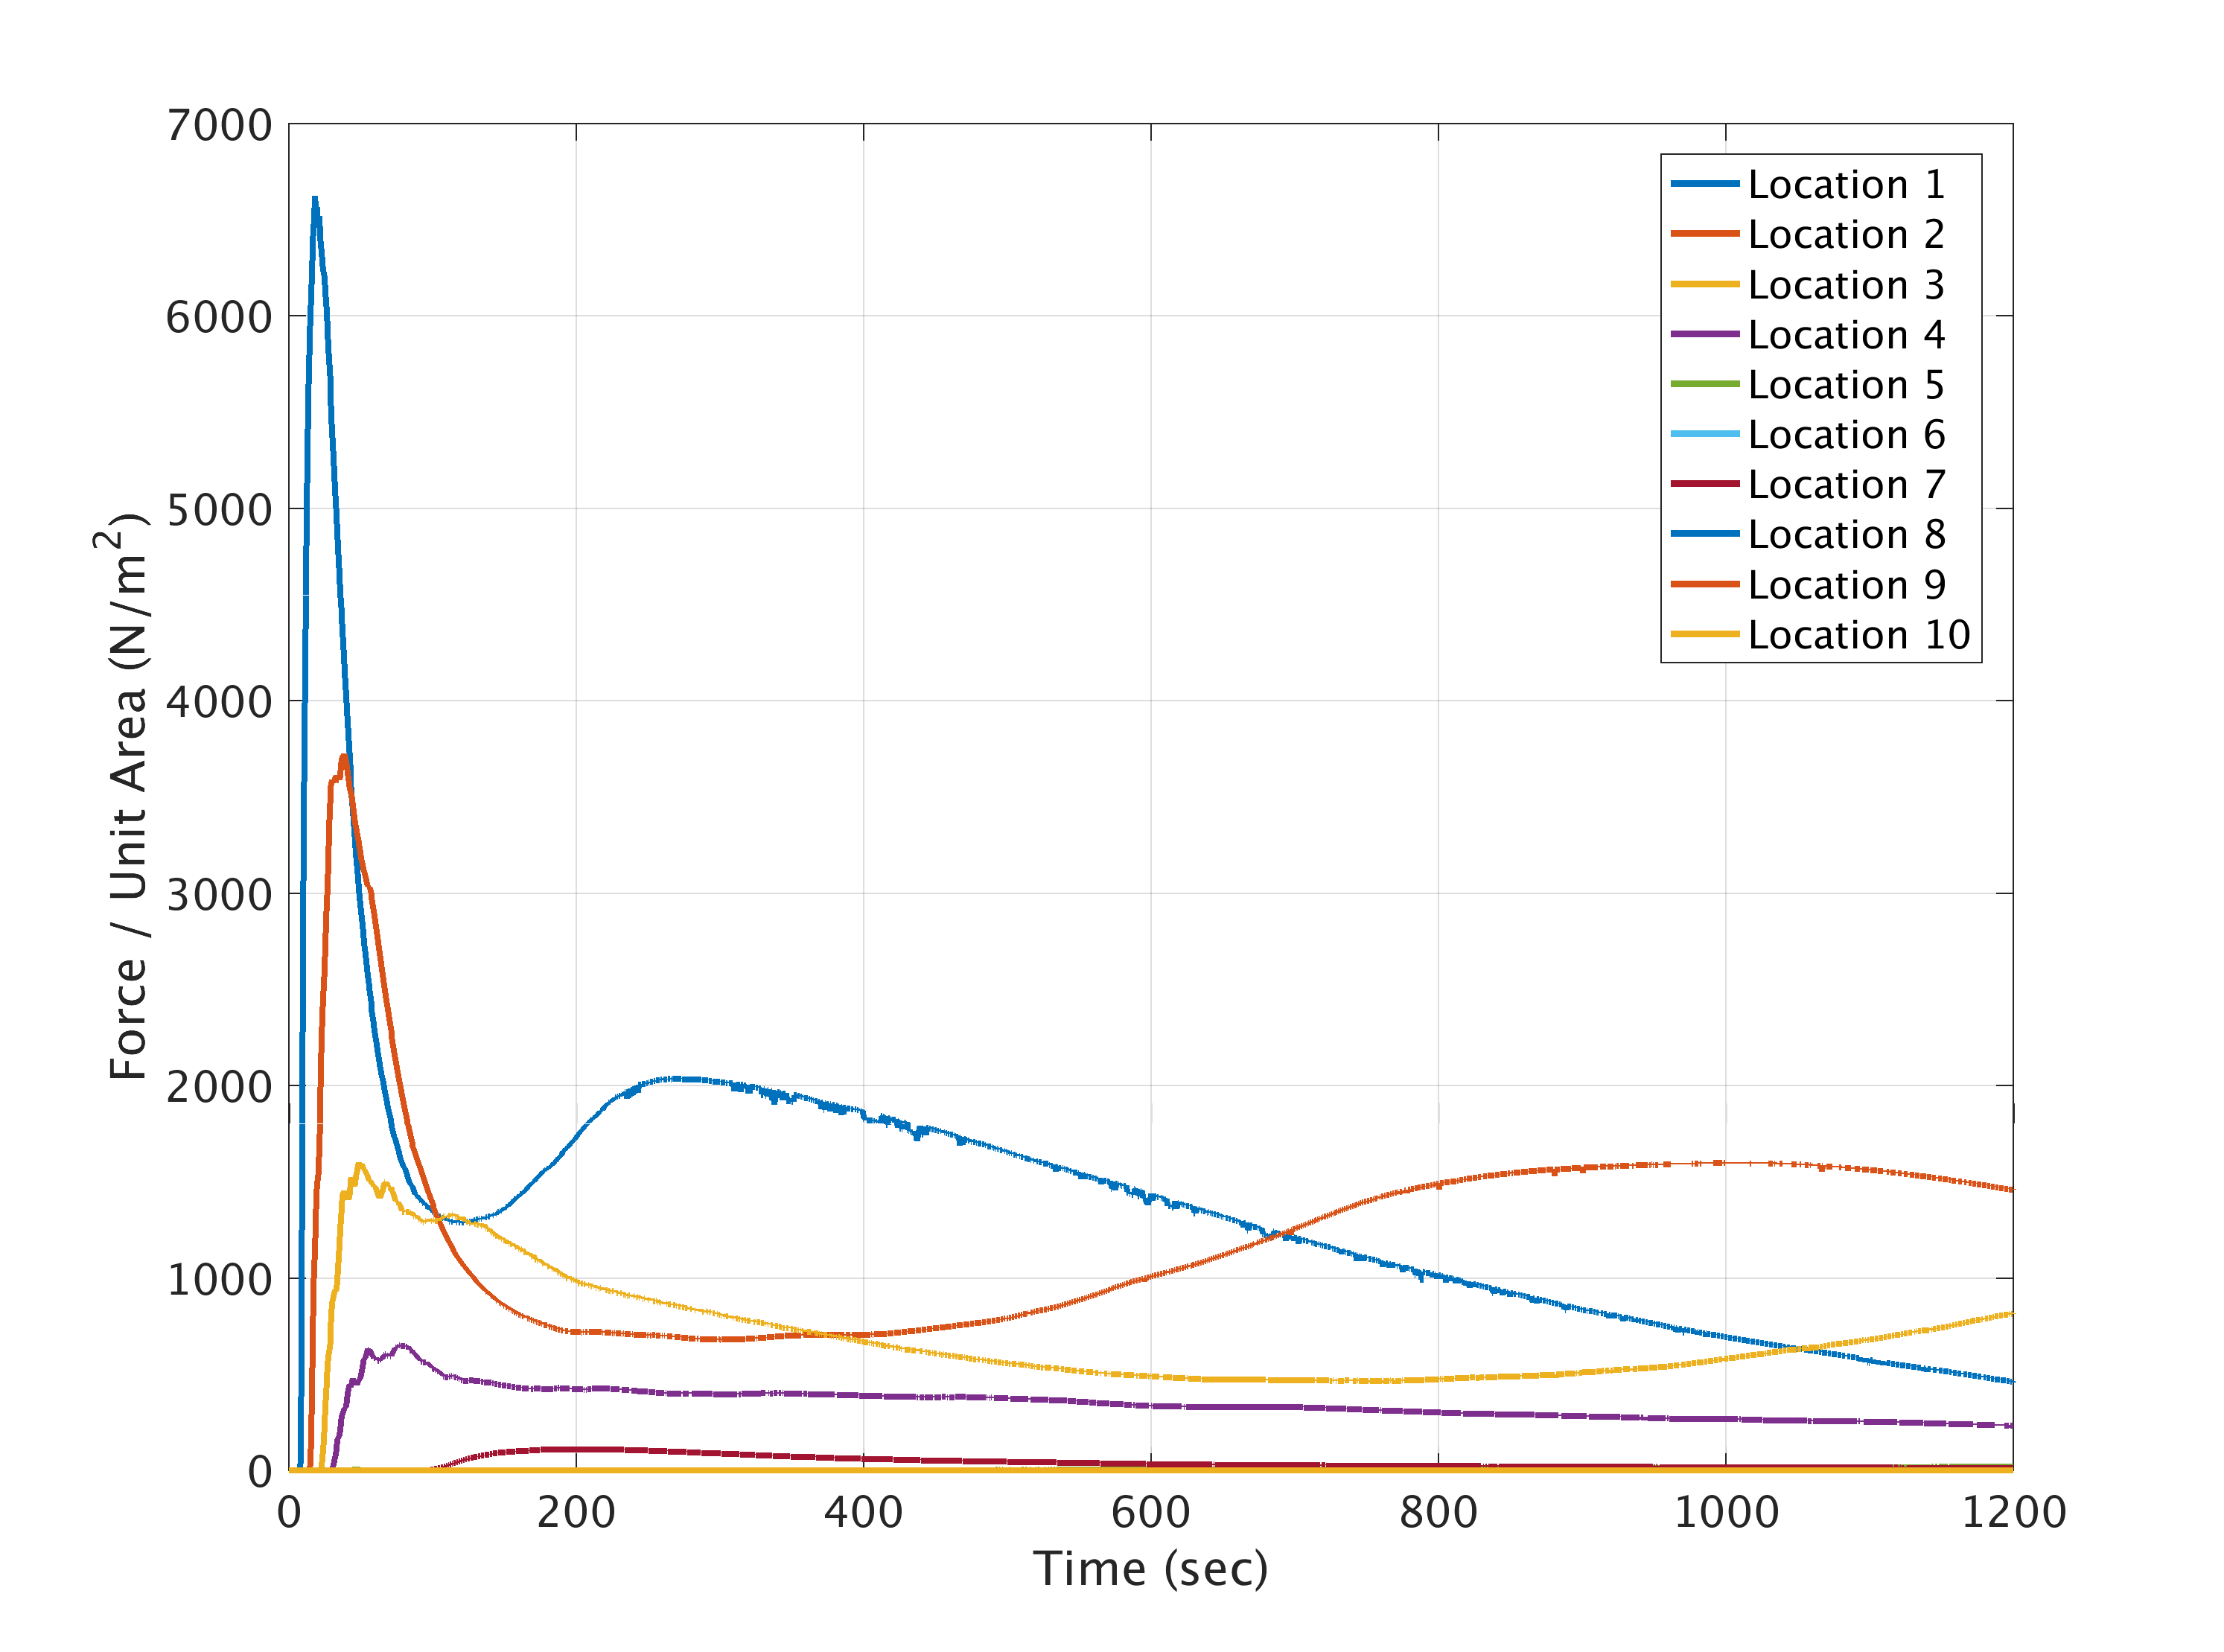
\includegraphics[width=1\textwidth]{MeansAll/FbedV_all.png}
        \subcaption{Bed Resisting Force Records, Voellmy-Salm.}
        \label{fig:M_FbVall}
	\end{minipage}

	\caption{Mean Values of gravitational and bed resisting force records at all the specified locations.}\label{fig:M_Fgball}
\end{figure}

\newpage
According to Figures \ref{fig:M_Fnet}, show that the mean values of net force records at the 10 specified locations for Mohr-Coulomb model are almost twice the mean values of Pouliquen-Forterre model, however, their values look almost similar after $\sim t=400-1200$ sec. On the other hand, in Voellmy-Salm model, mean values of the net force records seem to be even lower than the Pouliquen Forterre. This can justify the ``fast-moving'' nature of the Mohr-Coulomb model and why Voellmy-Salm model doesn't behave as a fast-moving rheology model. This low mean value record of net force for Voellmy-Salm model can also justify the ``material accumulation'' nature of this rheology.
\begin{figure}[H]

	\begin{minipage}[b]{0.5\linewidth}
	\centering
    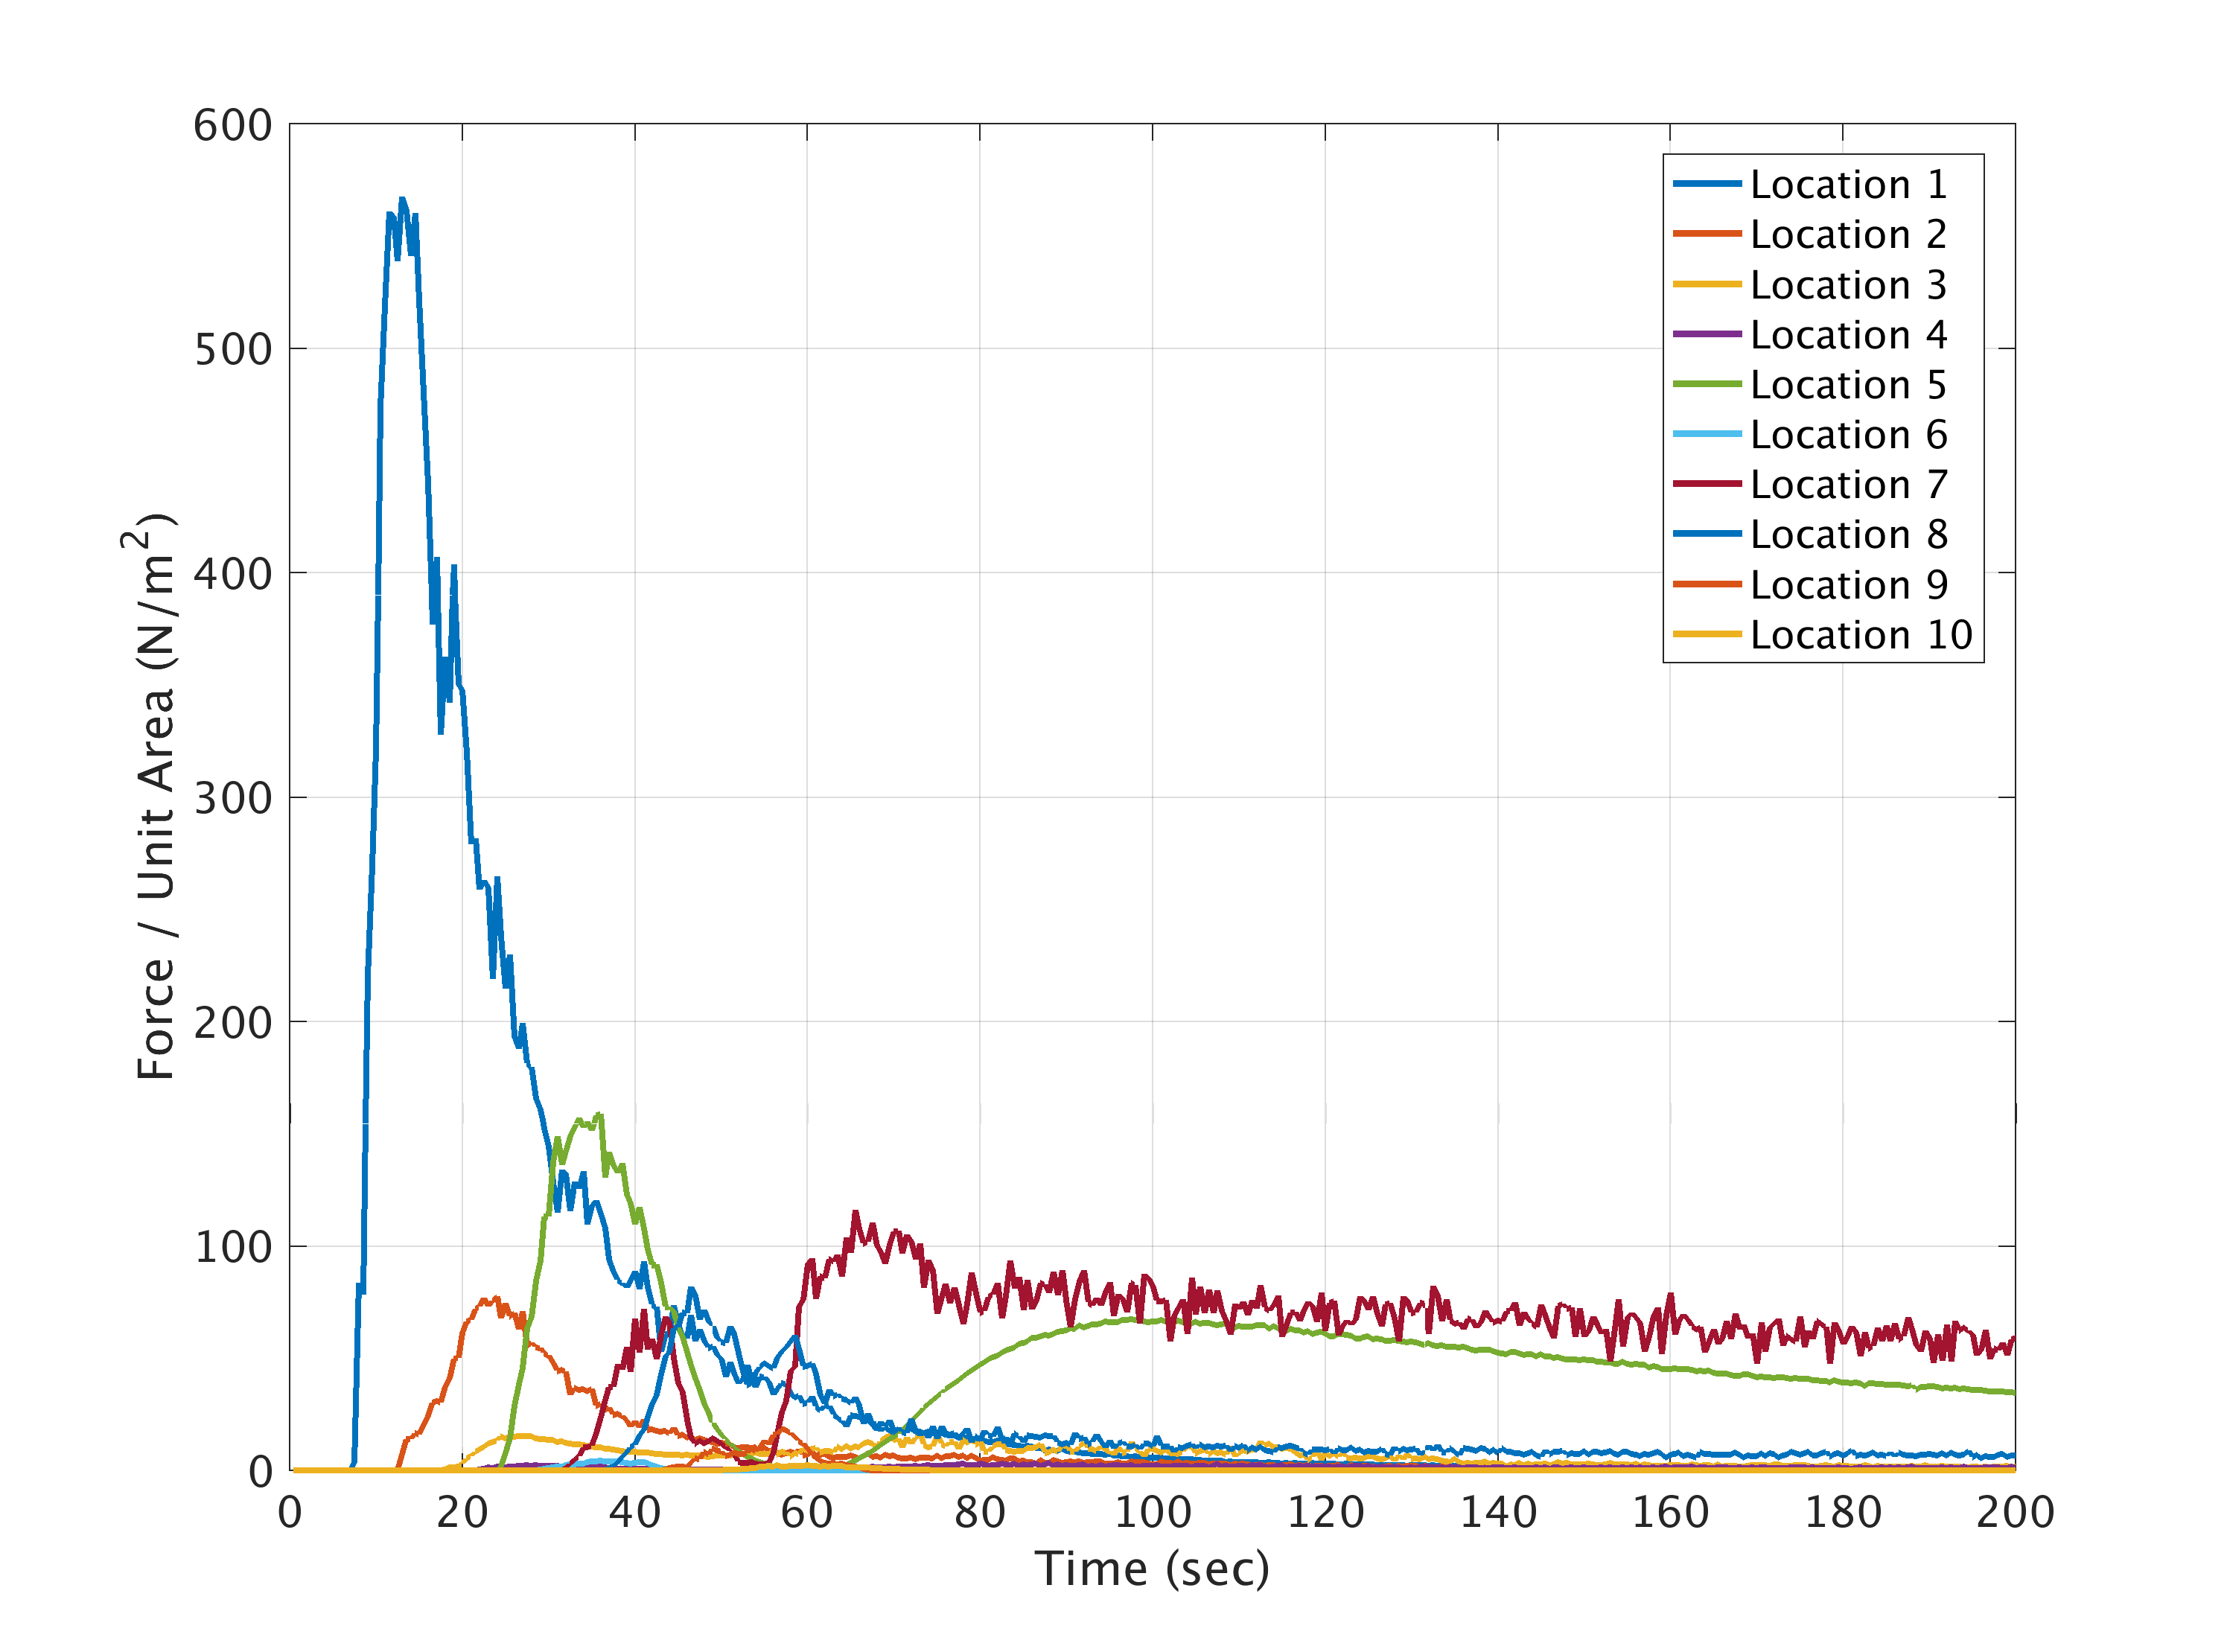
\includegraphics[width=1\textwidth]{MeansAll/FintC_all.png}     
        \subcaption{Internal friction force records, Mohr-Coulomb.}
        \label{fig:M_FintCall}
	\end{minipage}
	\begin{minipage}[b]{0.5\linewidth}
	\centering
    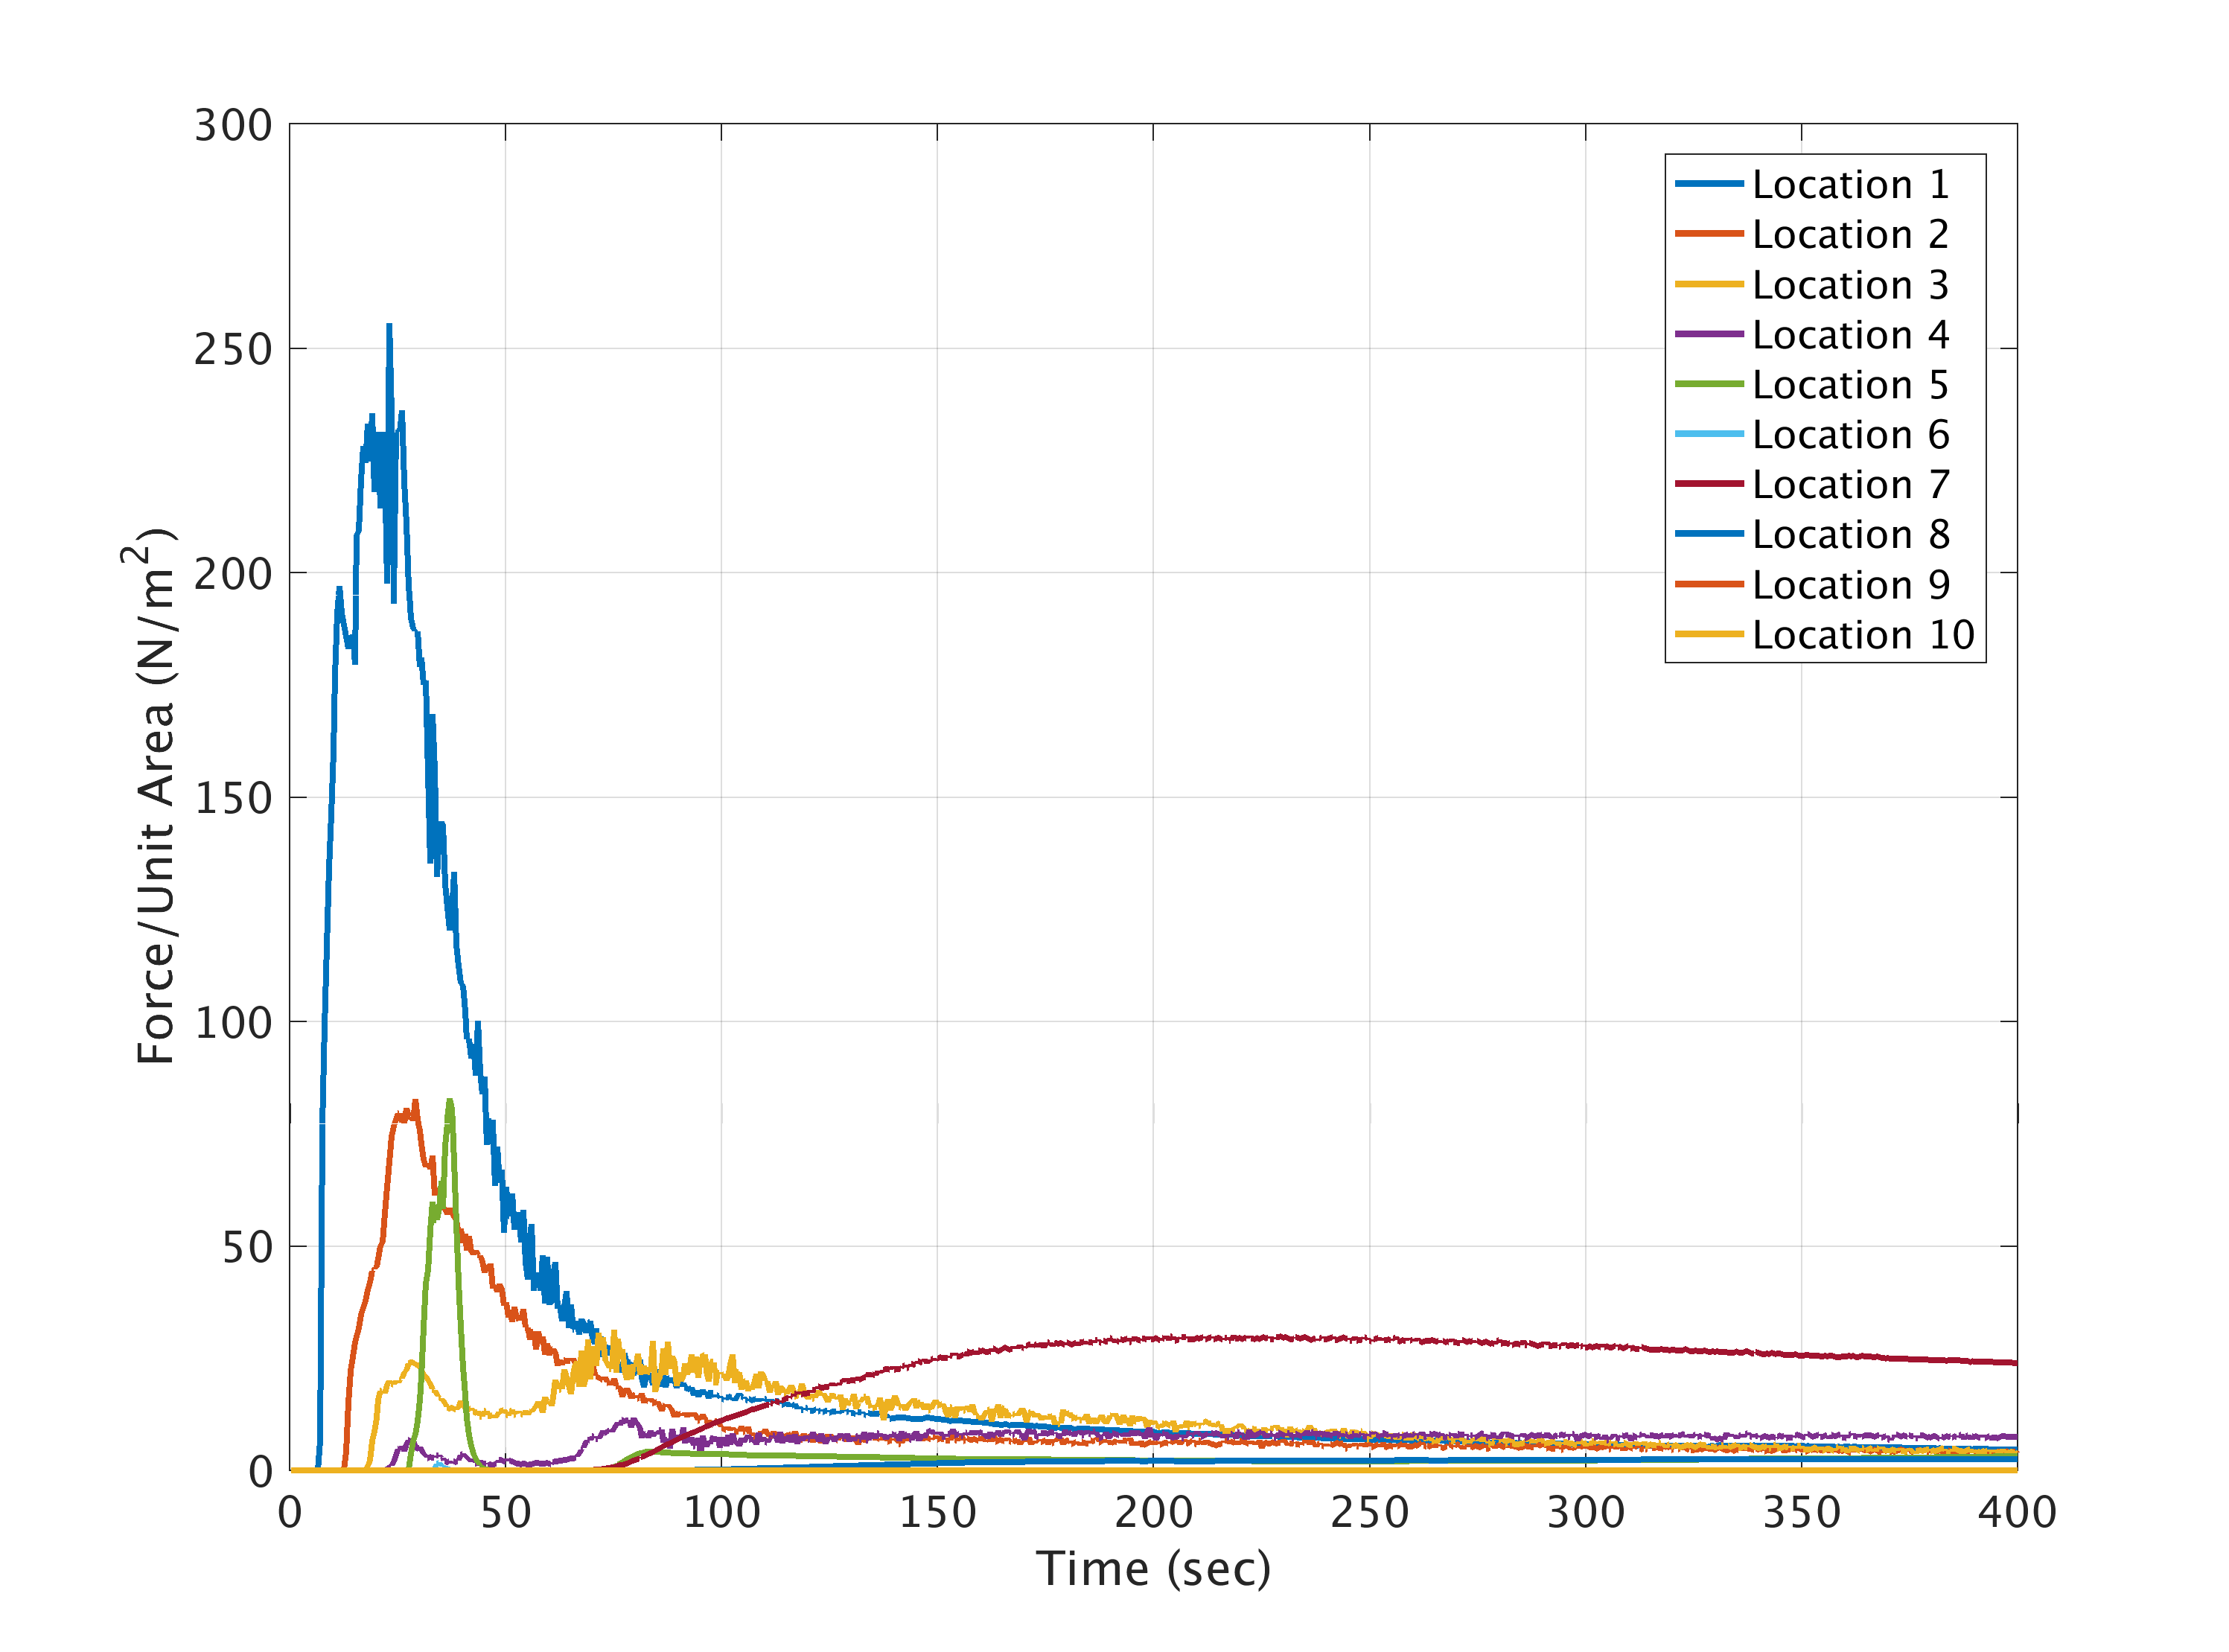
\includegraphics[width=1\textwidth]{MeansAll/FpressP_all.png}
        \subcaption{Pressure gradient force records, Pouliquen-Forterre.}
        \label{fig:M_FpressPall}
	\end{minipage}
	
	\begin{minipage}[b]{1\linewidth}
	\centering
    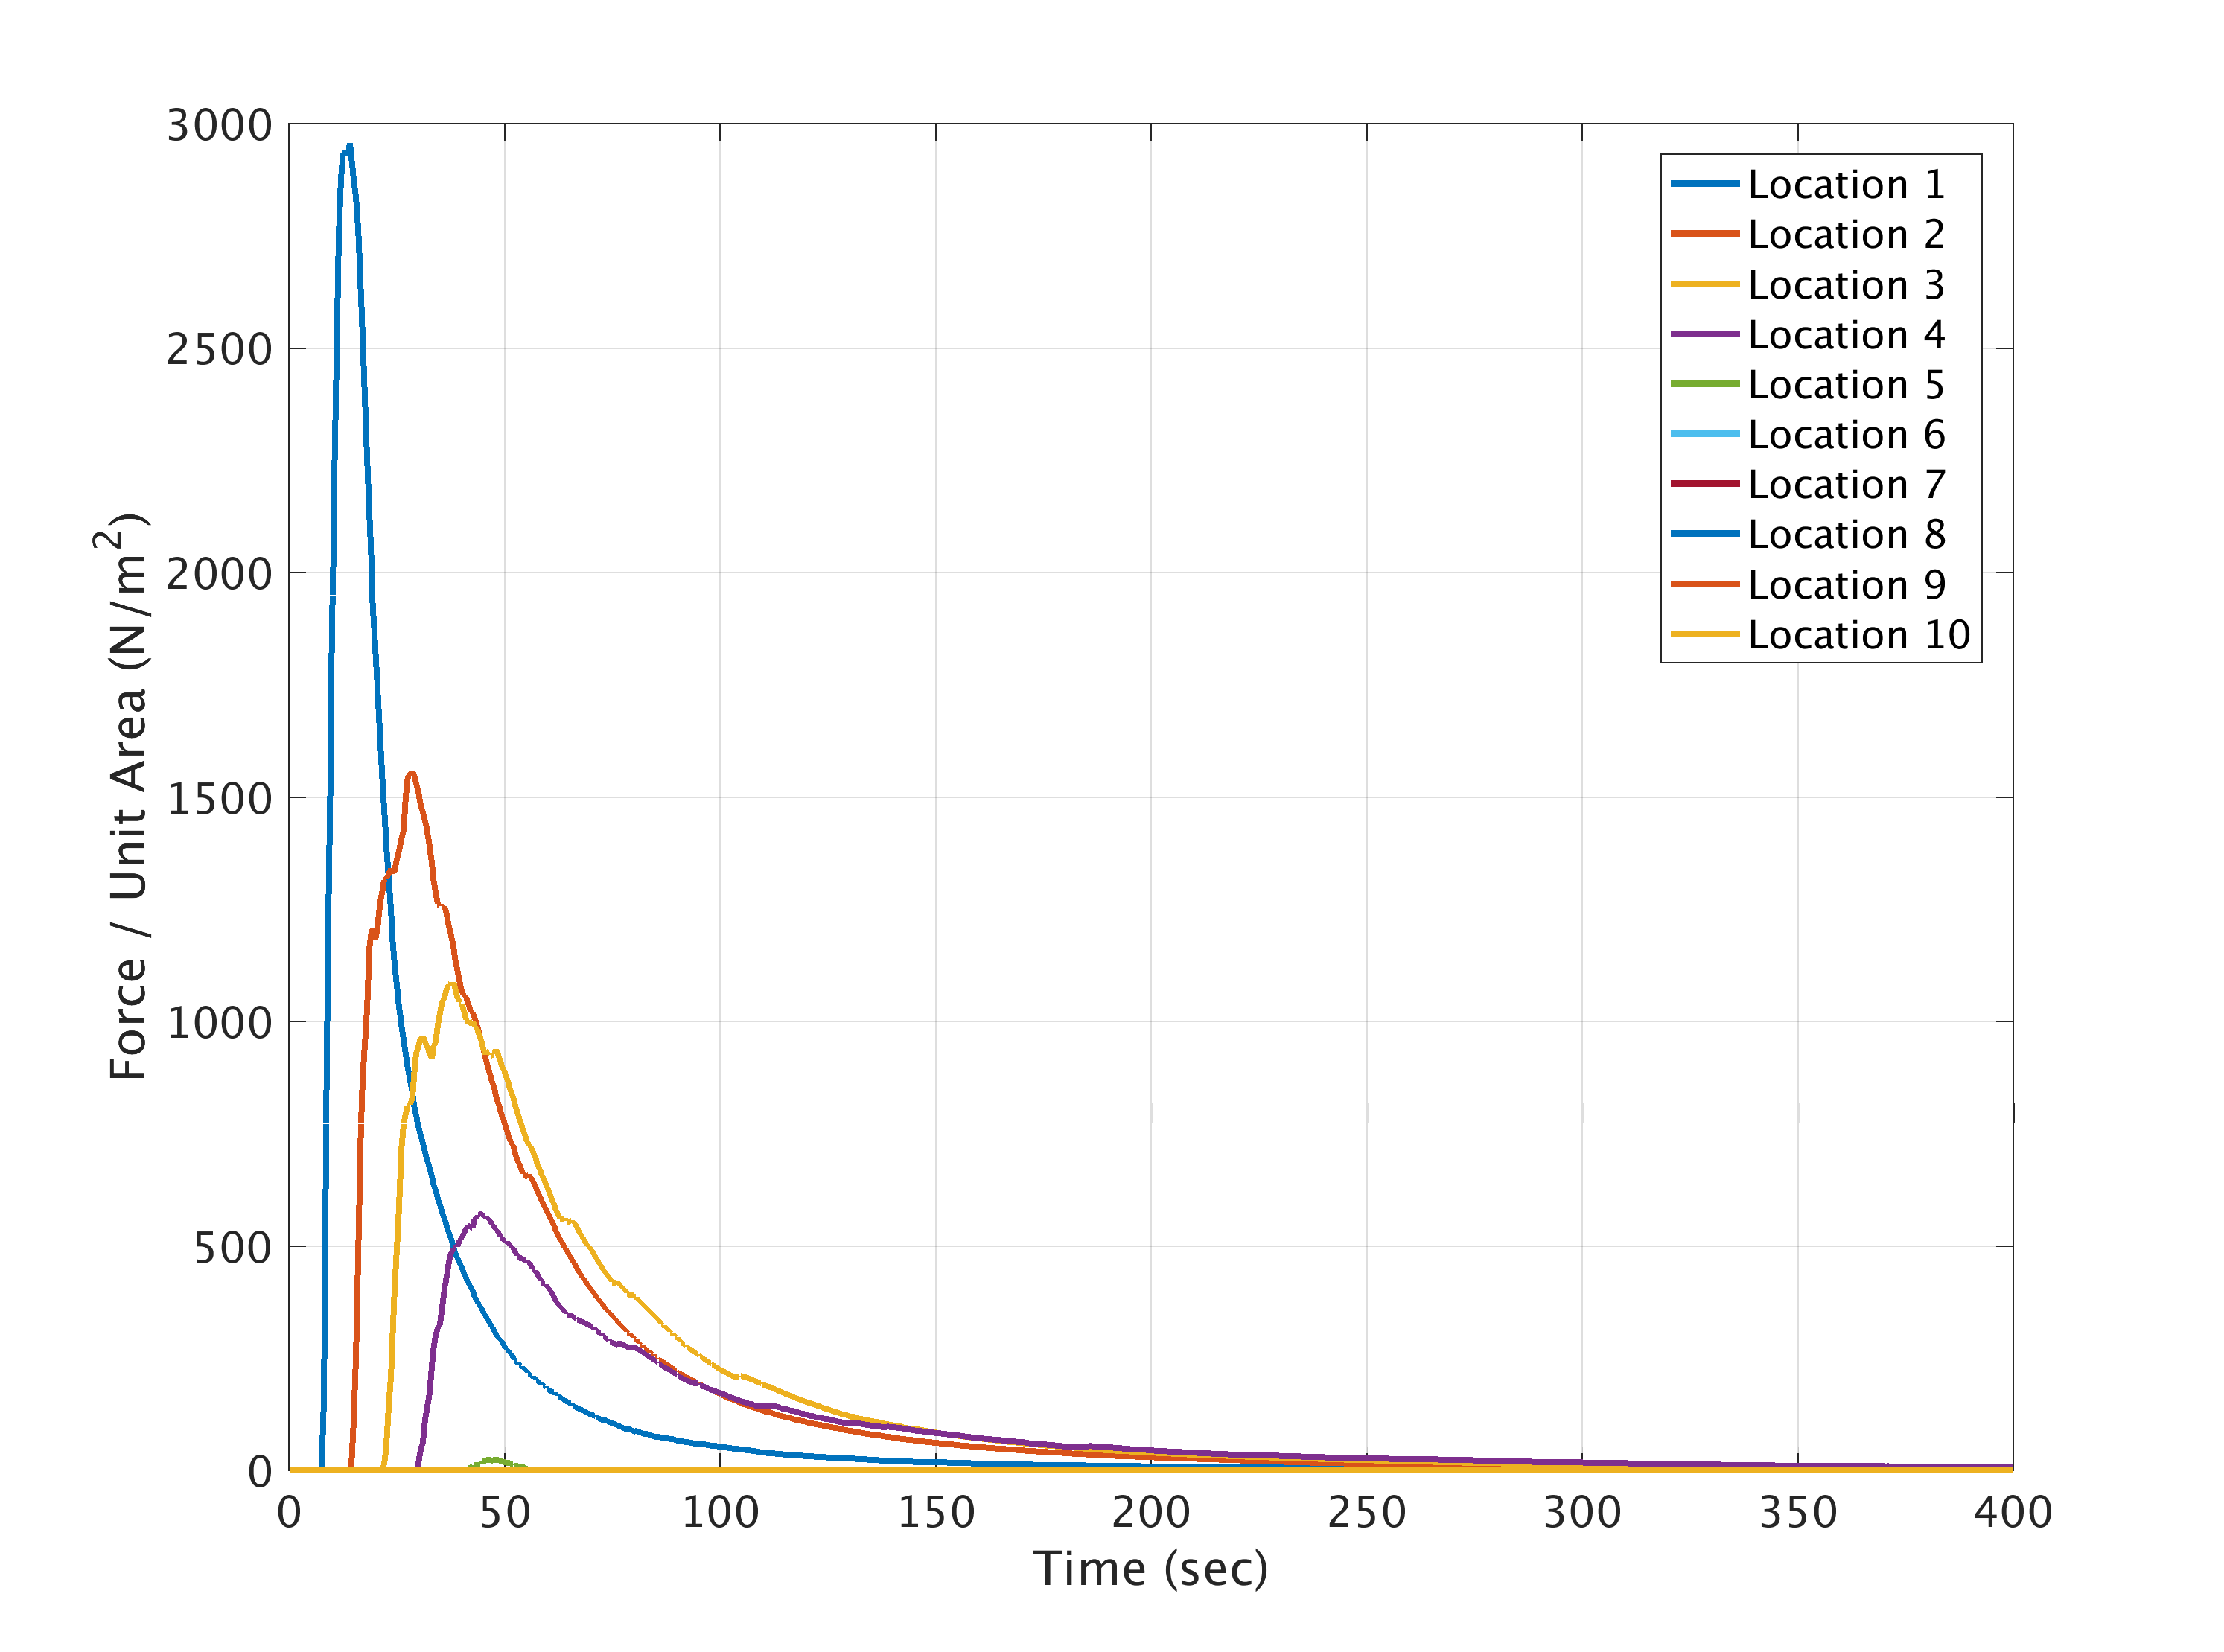
\includegraphics[width=0.5\textwidth]{MeansAll/FviscV_all.png}
        \subcaption{Viscouse force records, Voellmy-Salm.}
        \label{fig:M_FviscVall}
	\end{minipage}
				
	\caption{Mean Values of other source of resisting force records at all the specified locations.}\label{fig:M_FoCall}	
\end{figure}

\subsection{Records at each location}\label{sec:MV_loc}

\begin{figure}[H]
	\begin{minipage}[b]{0.5\linewidth}
	\centering
    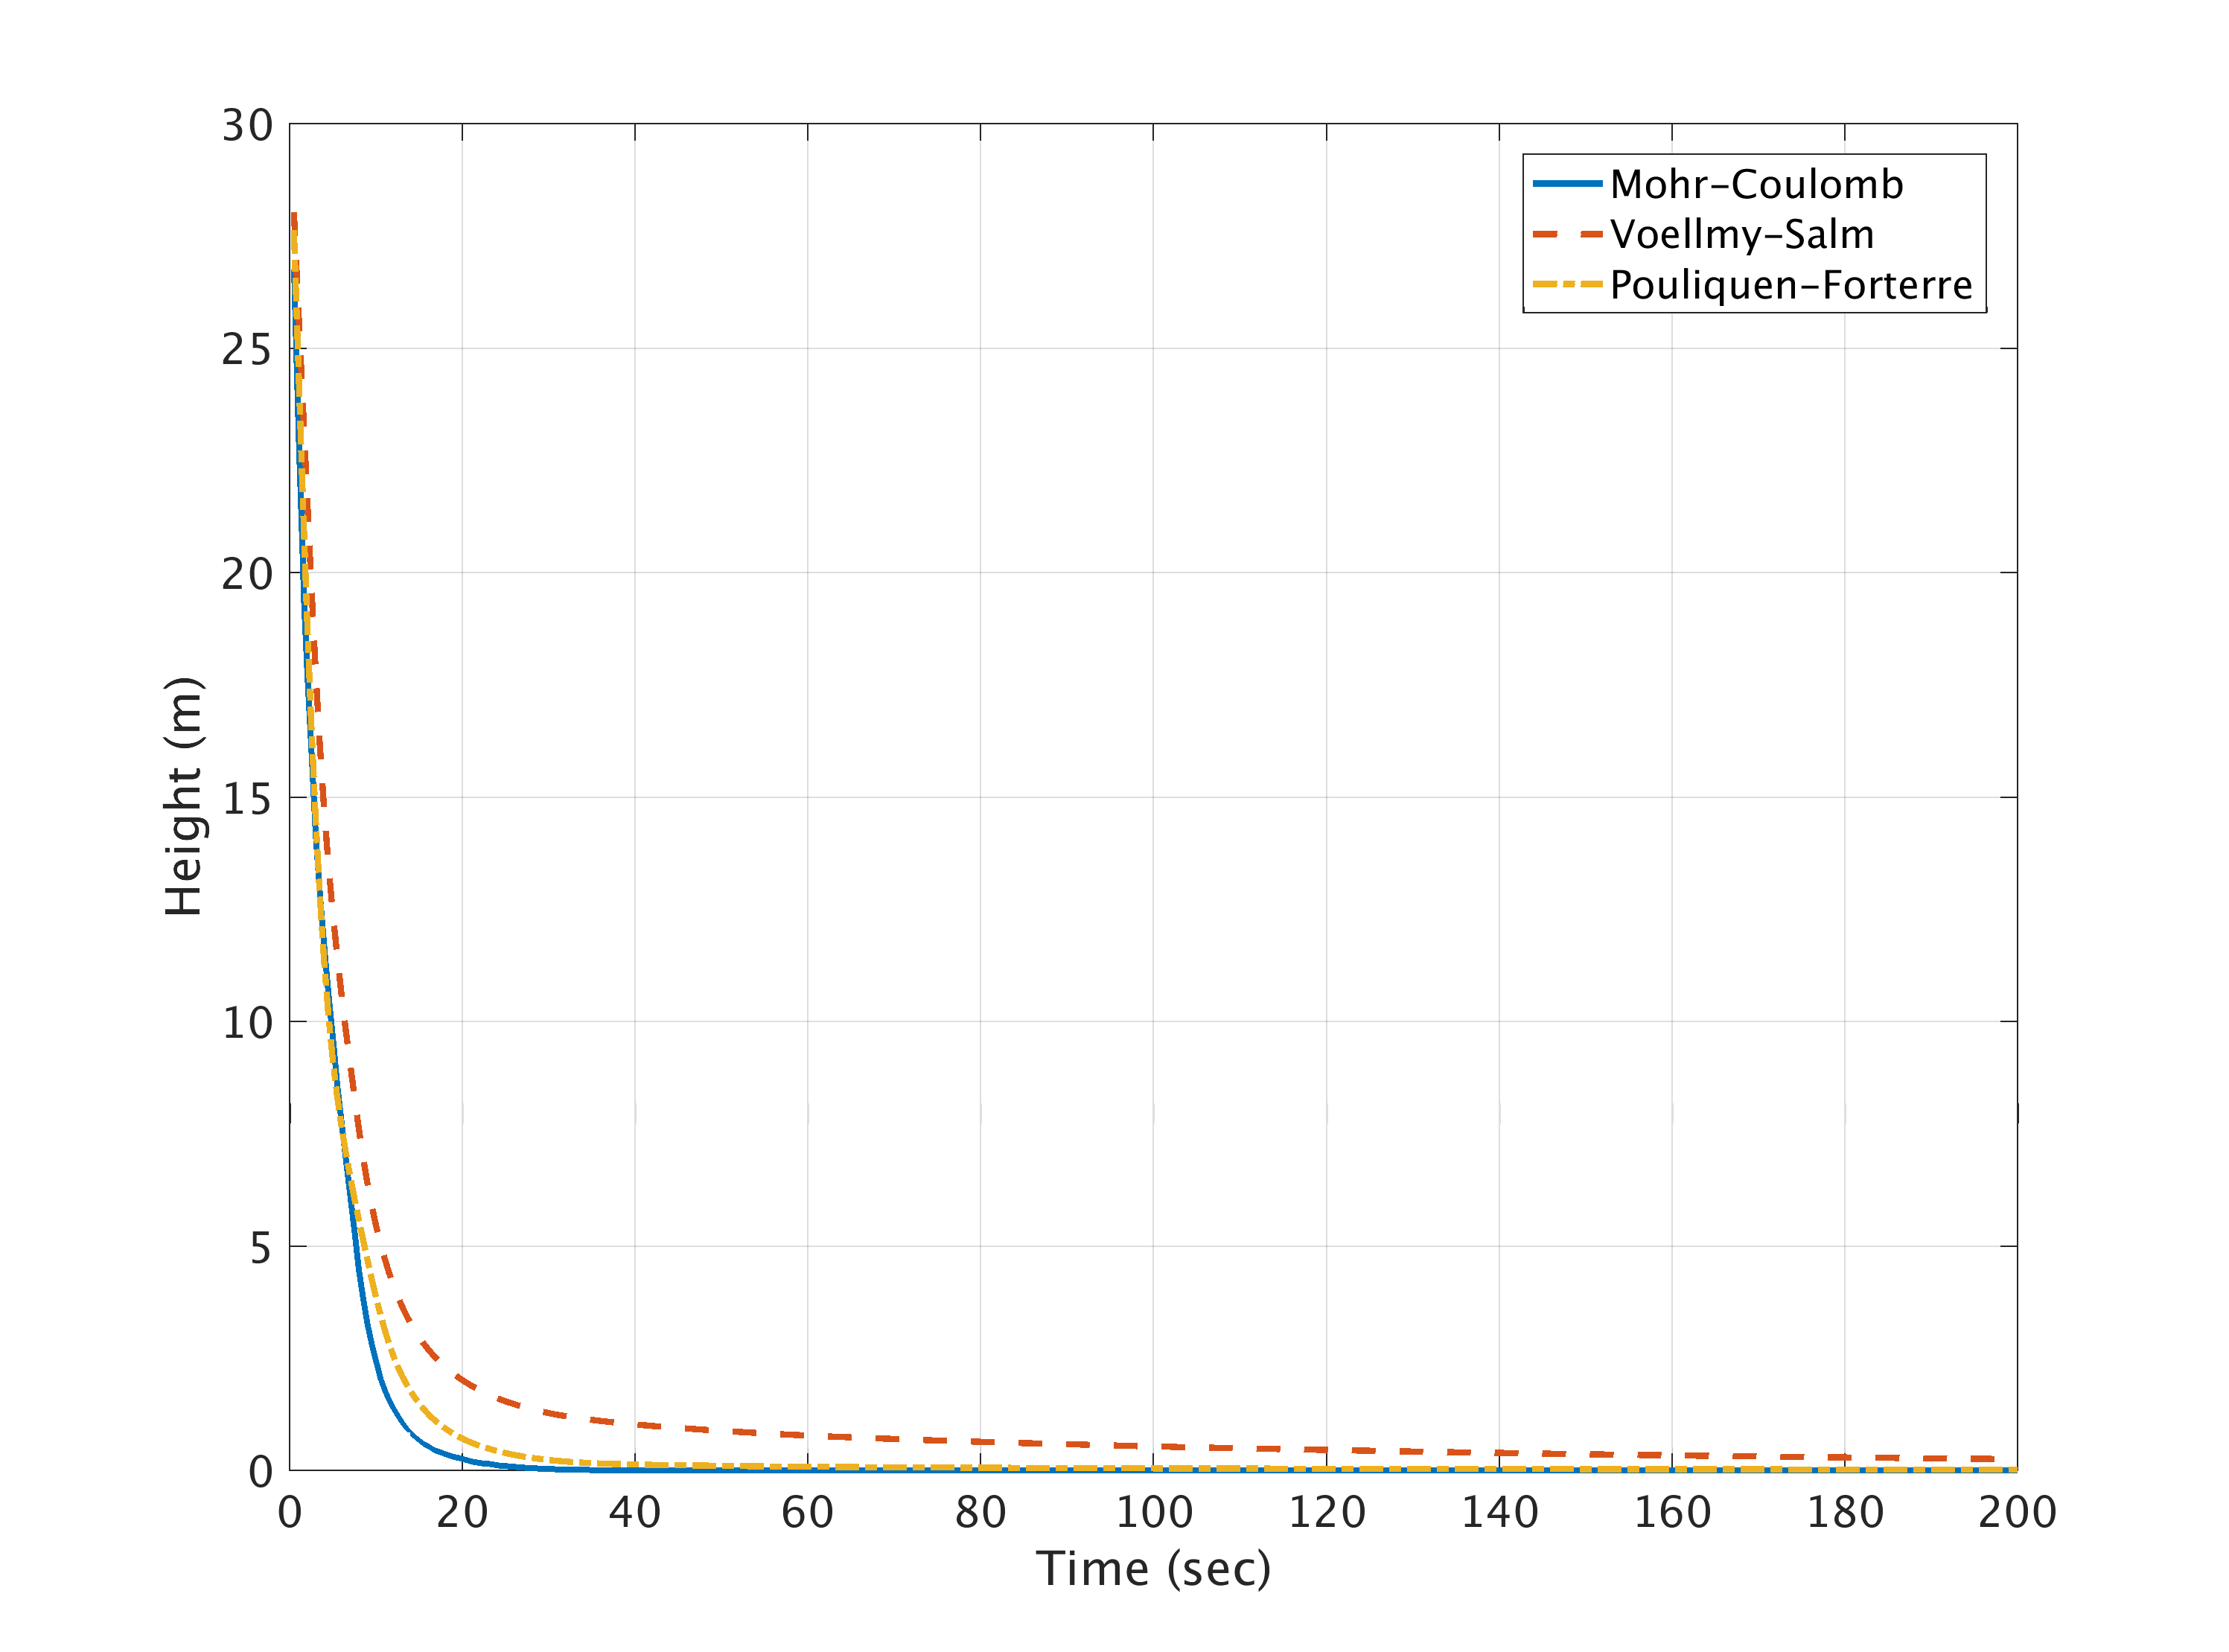
\includegraphics[width=1\textwidth]{HeightMeans/H1All.png}     
        \subcaption{Flow Height Records, Location 1.}
        \label{fig:MFHR_L1}
	\end{minipage}
	\begin{minipage}[b]{0.5\linewidth}
	\centering
    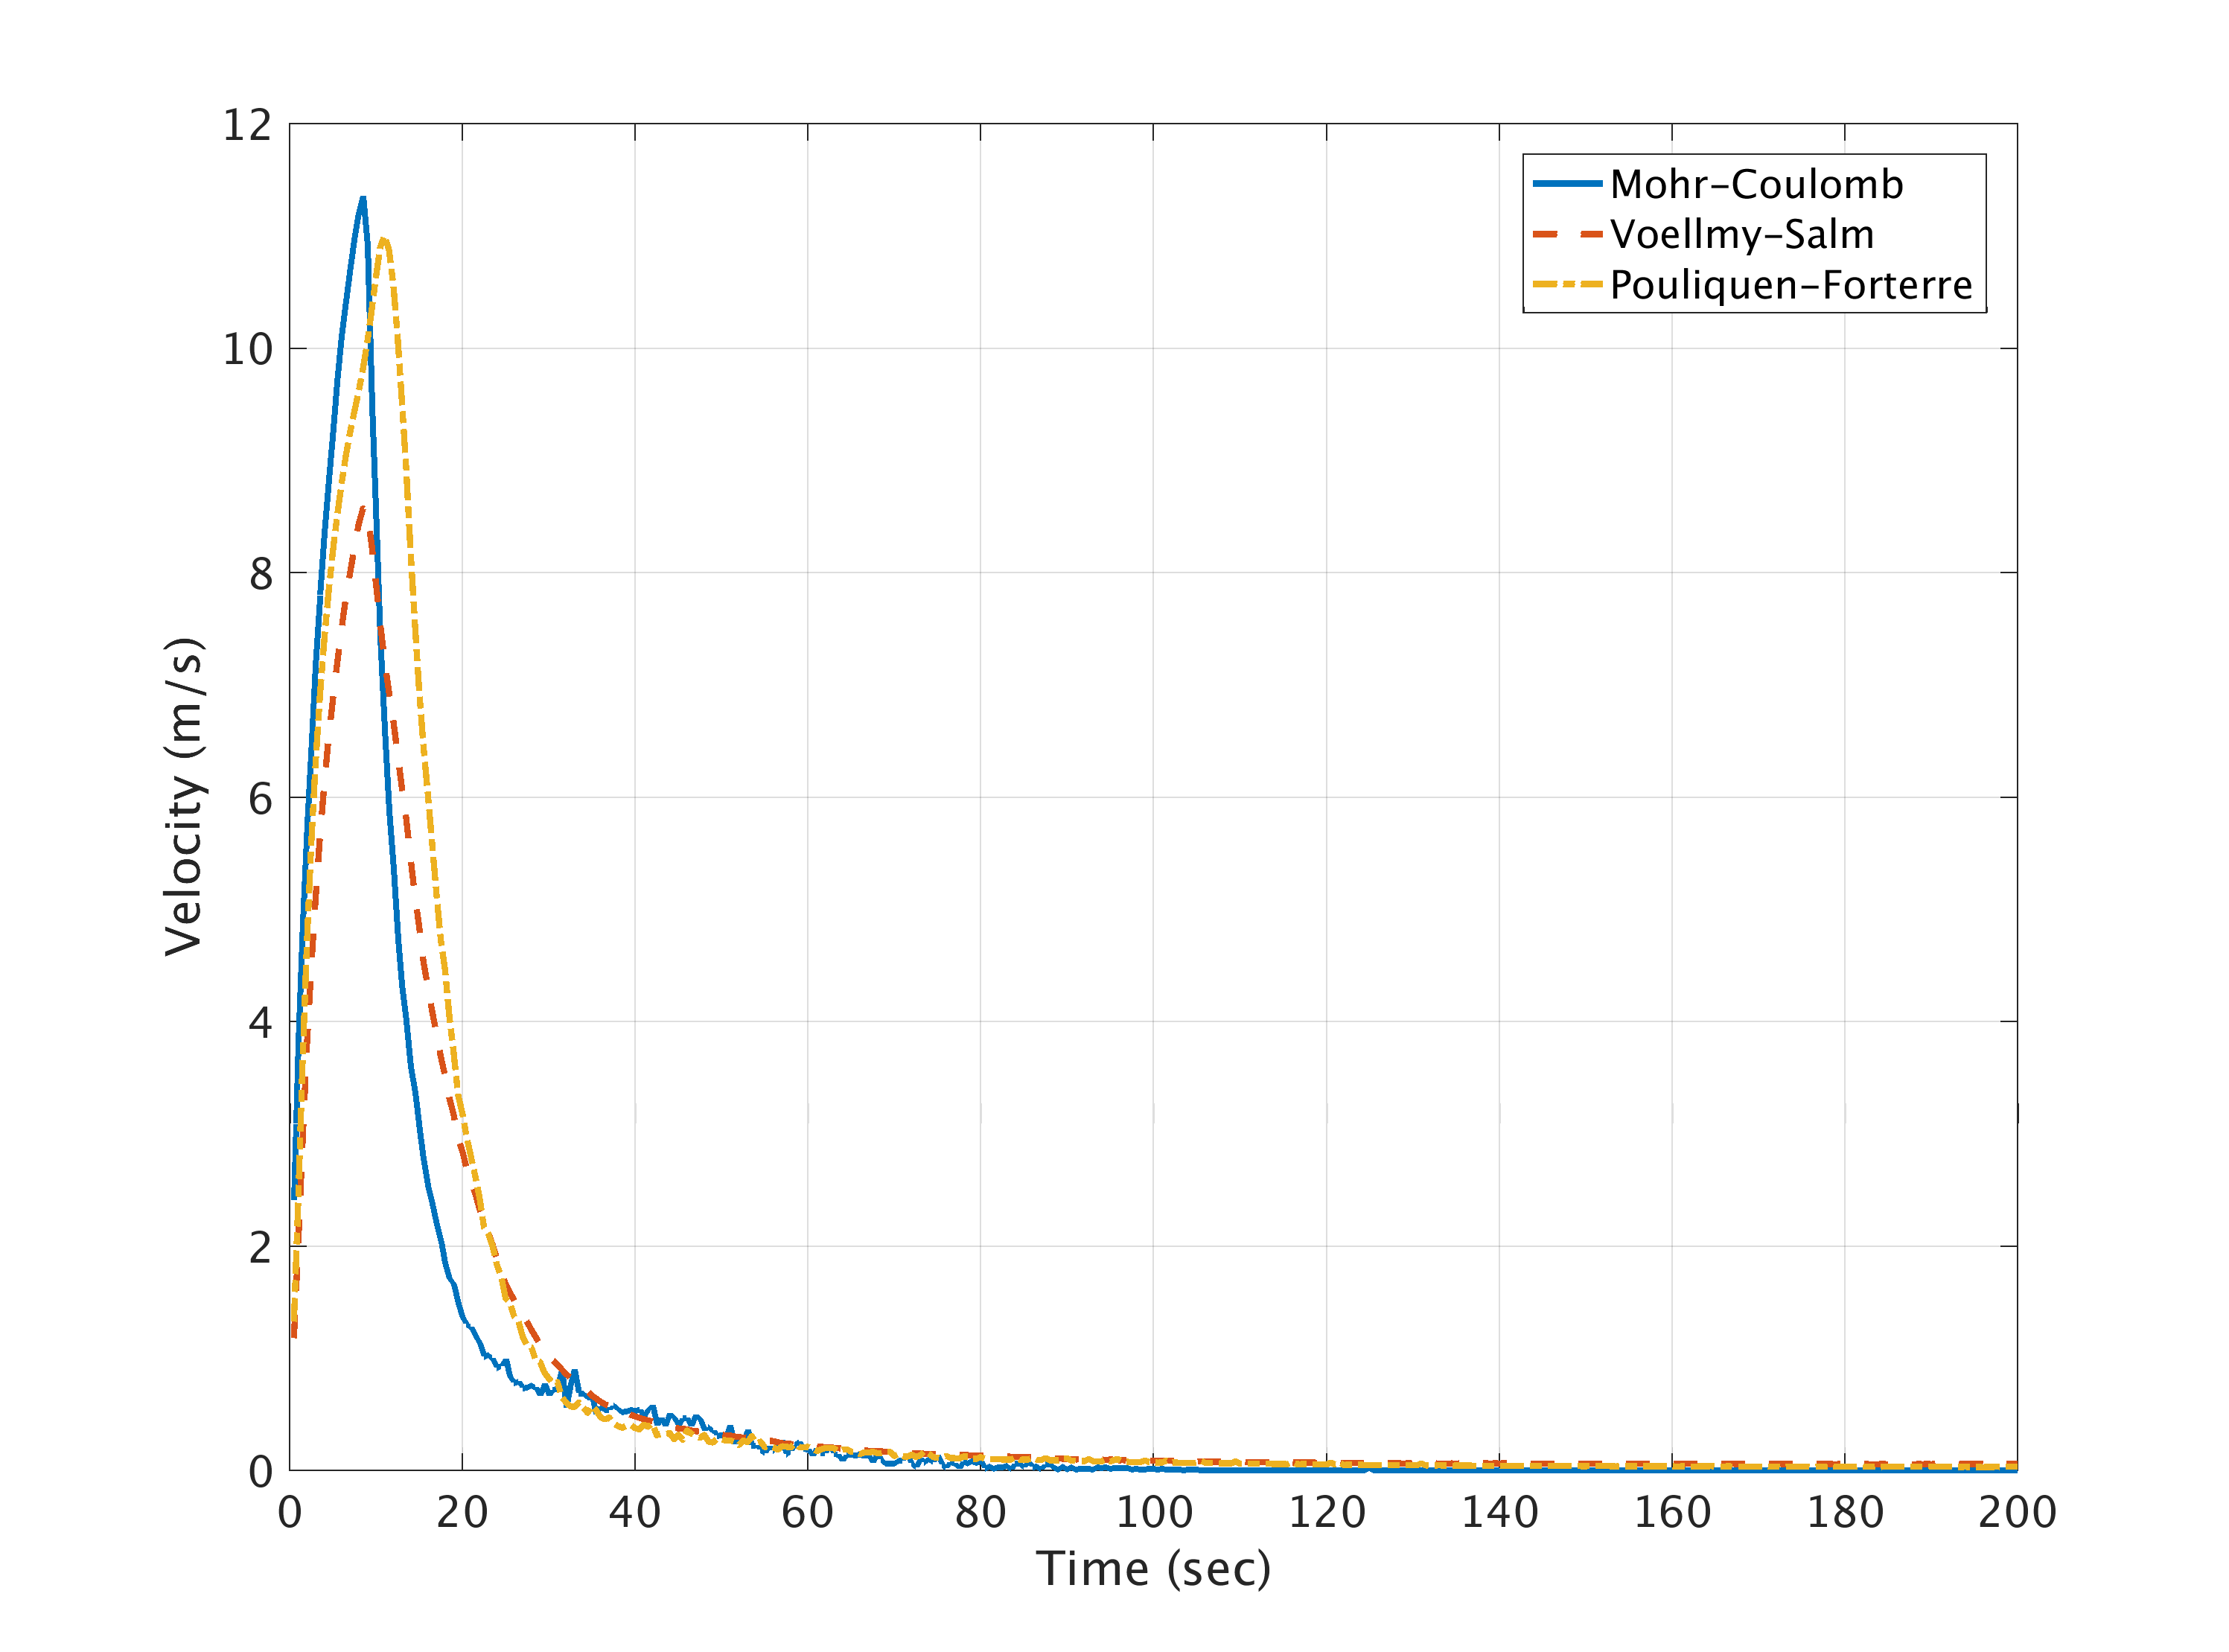
\includegraphics[width=1\textwidth]{VelocityMeans/V1All.png}
        \subcaption{Flow Velocity Records, Location 1.}
        \label{fig:MFVR_L1}
	\end{minipage}
	
	\begin{minipage}[b]{0.5\linewidth}
	\centering
    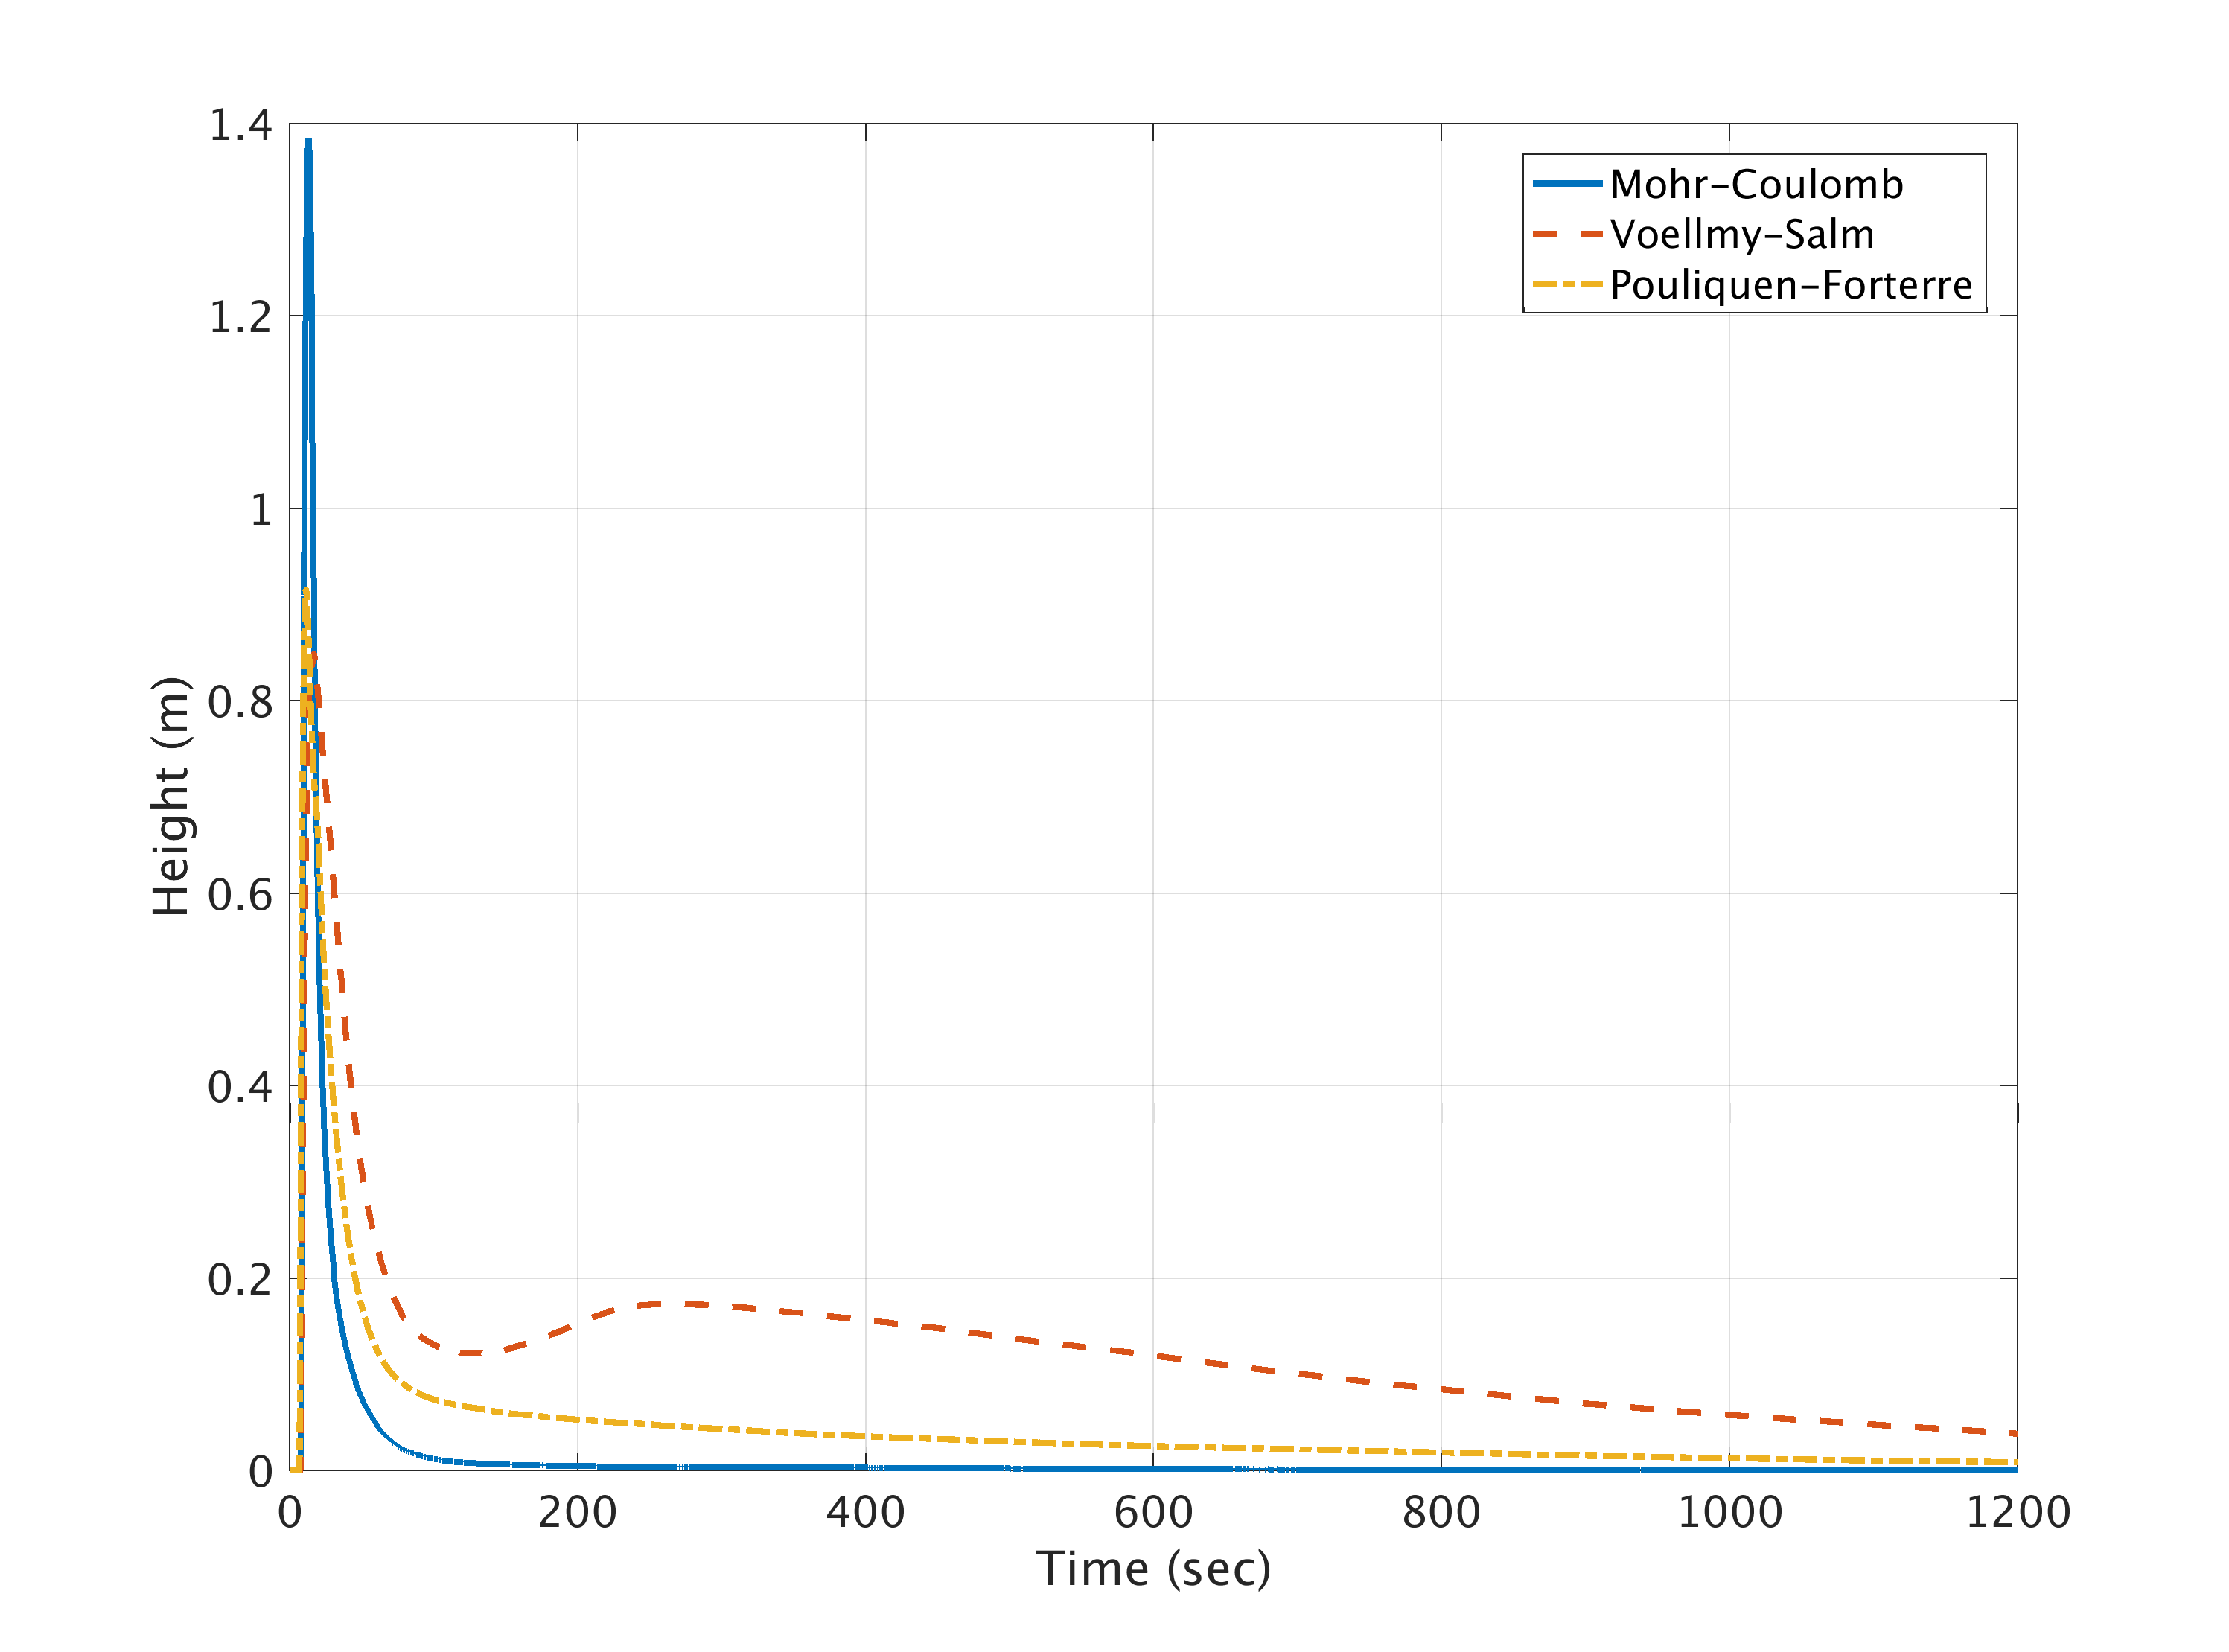
\includegraphics[width=1\textwidth]{HeightMeans/H2All.png}     
        \subcaption{Flow Height Records, Location 2.}
        \label{fig:MFHR_L2}
	\end{minipage}
	\begin{minipage}[b]{0.5\linewidth}
	\centering
    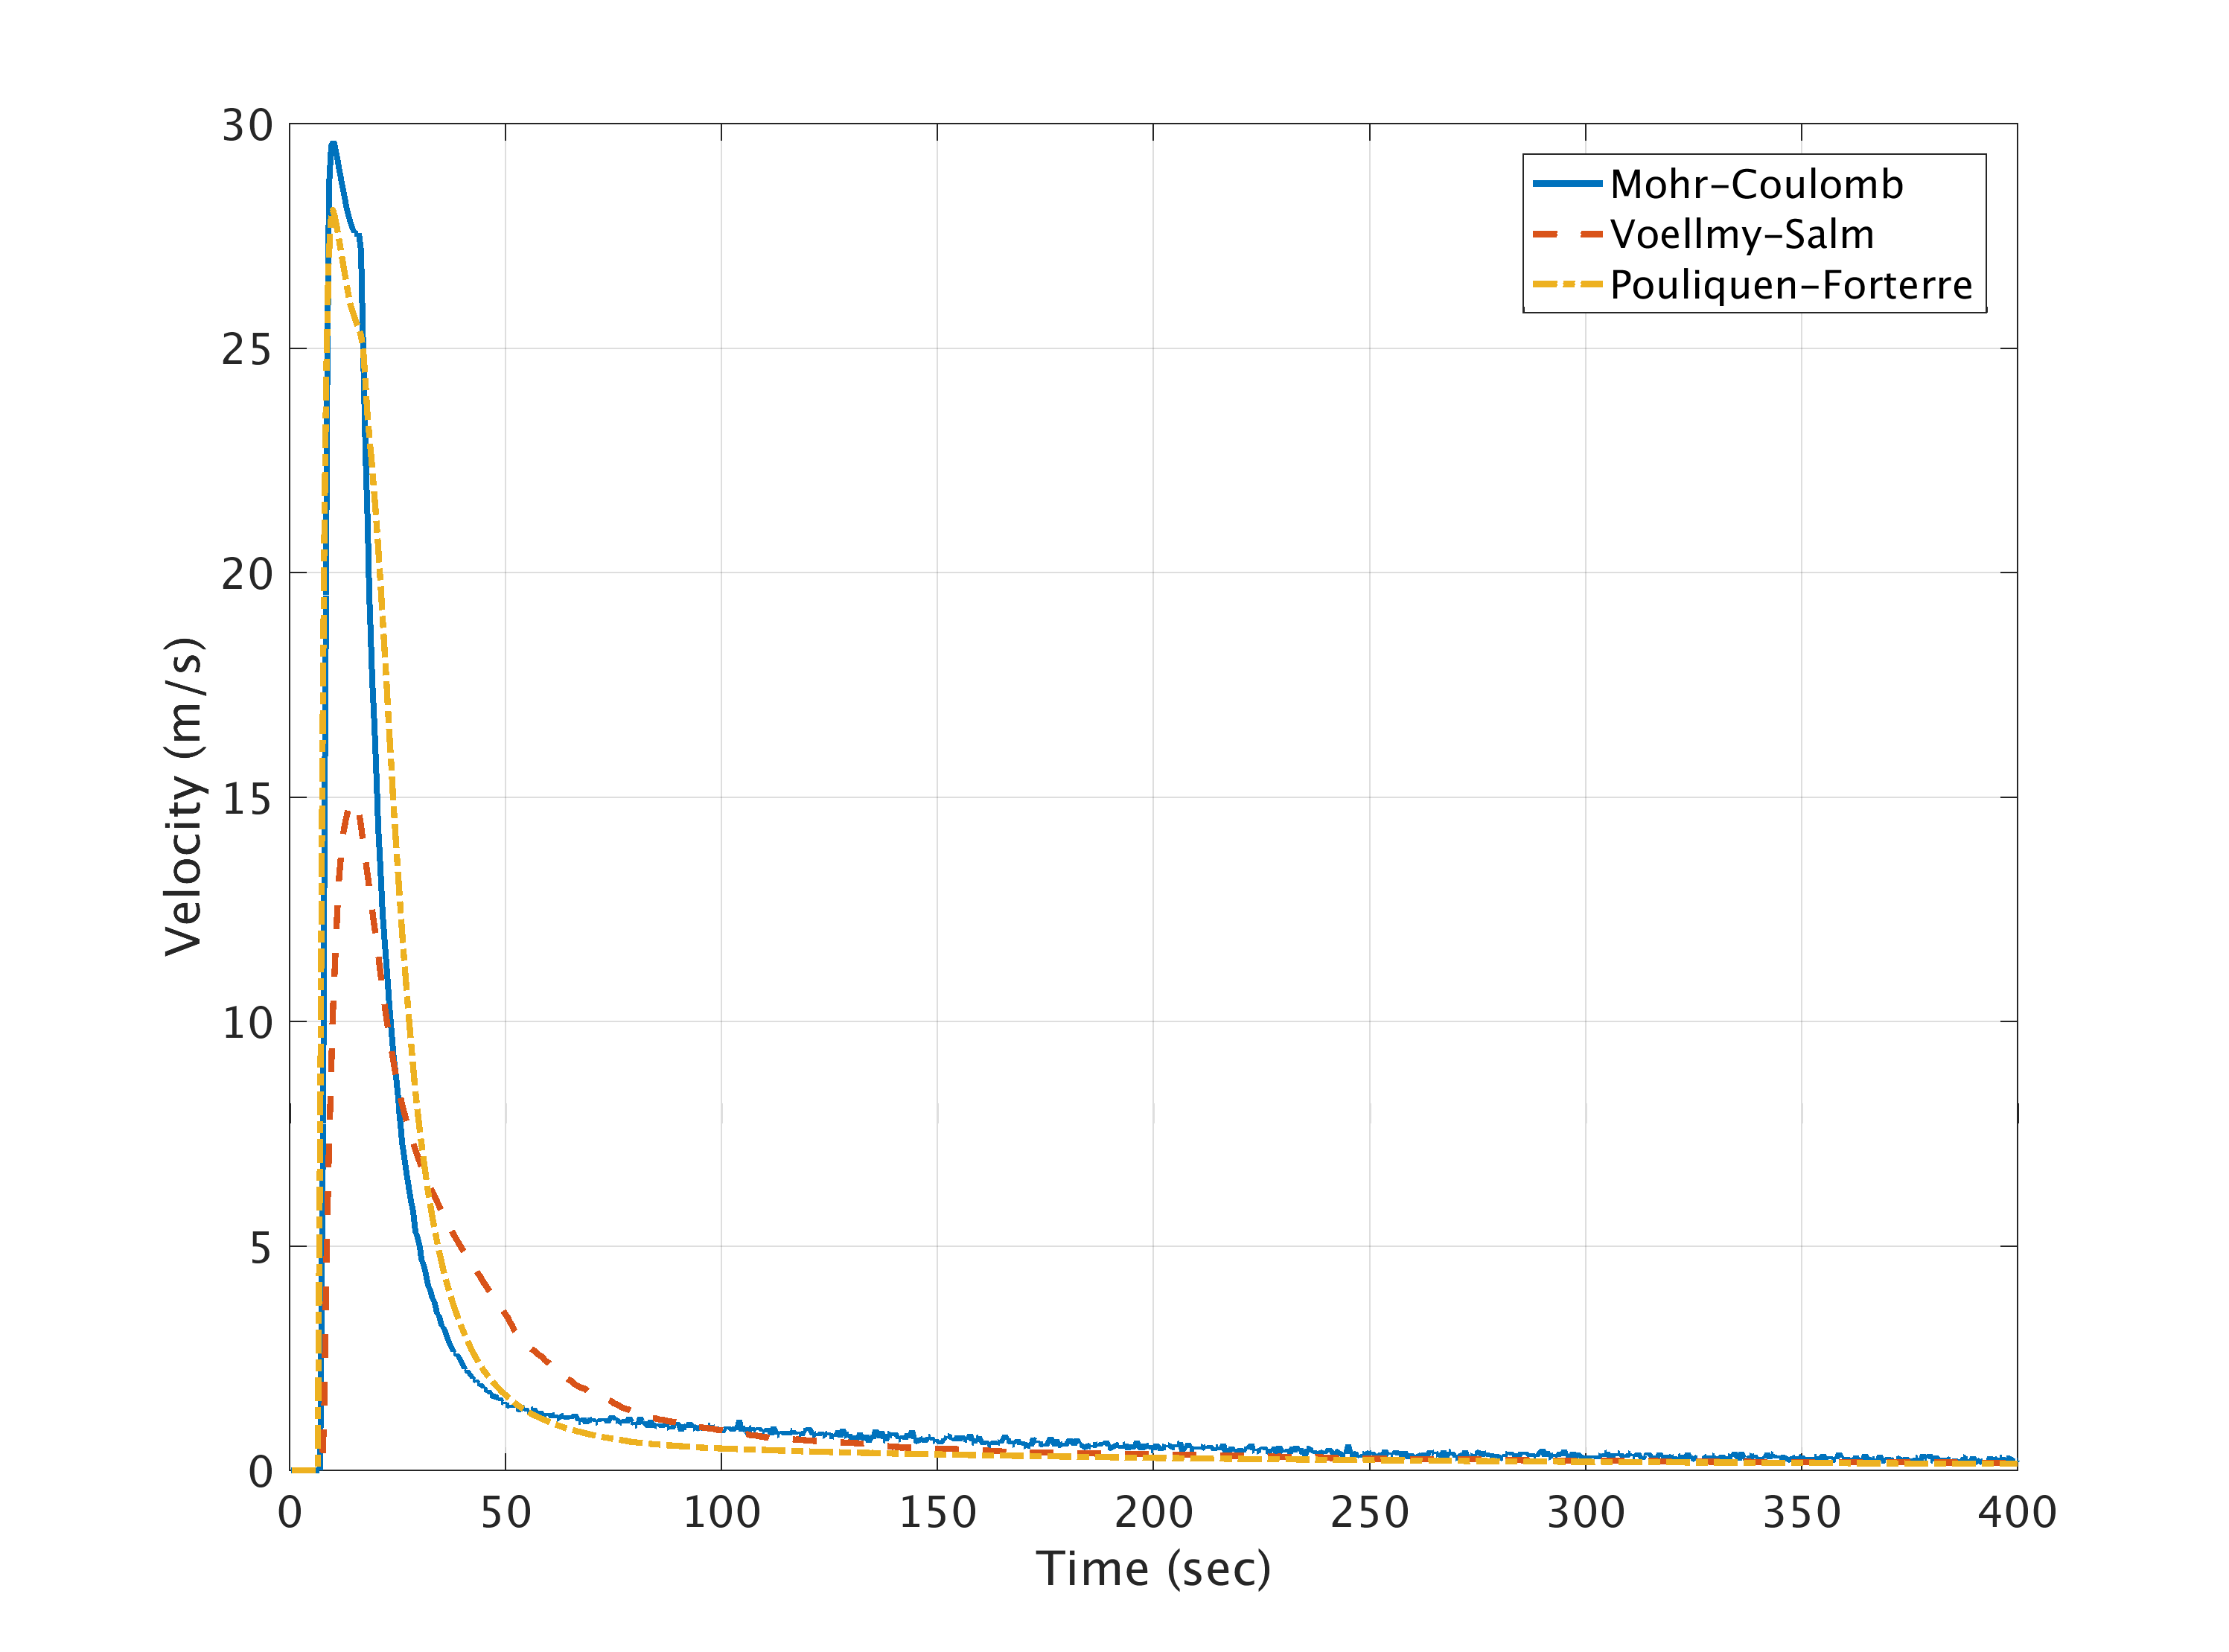
\includegraphics[width=1\textwidth]{VelocityMeans/V2All.png}
        \subcaption{Flow Velocity Records, Location 2.}
        \label{fig:MFVR_L2}
	\end{minipage}
	
	\begin{minipage}[b]{0.5\linewidth}
	\centering
    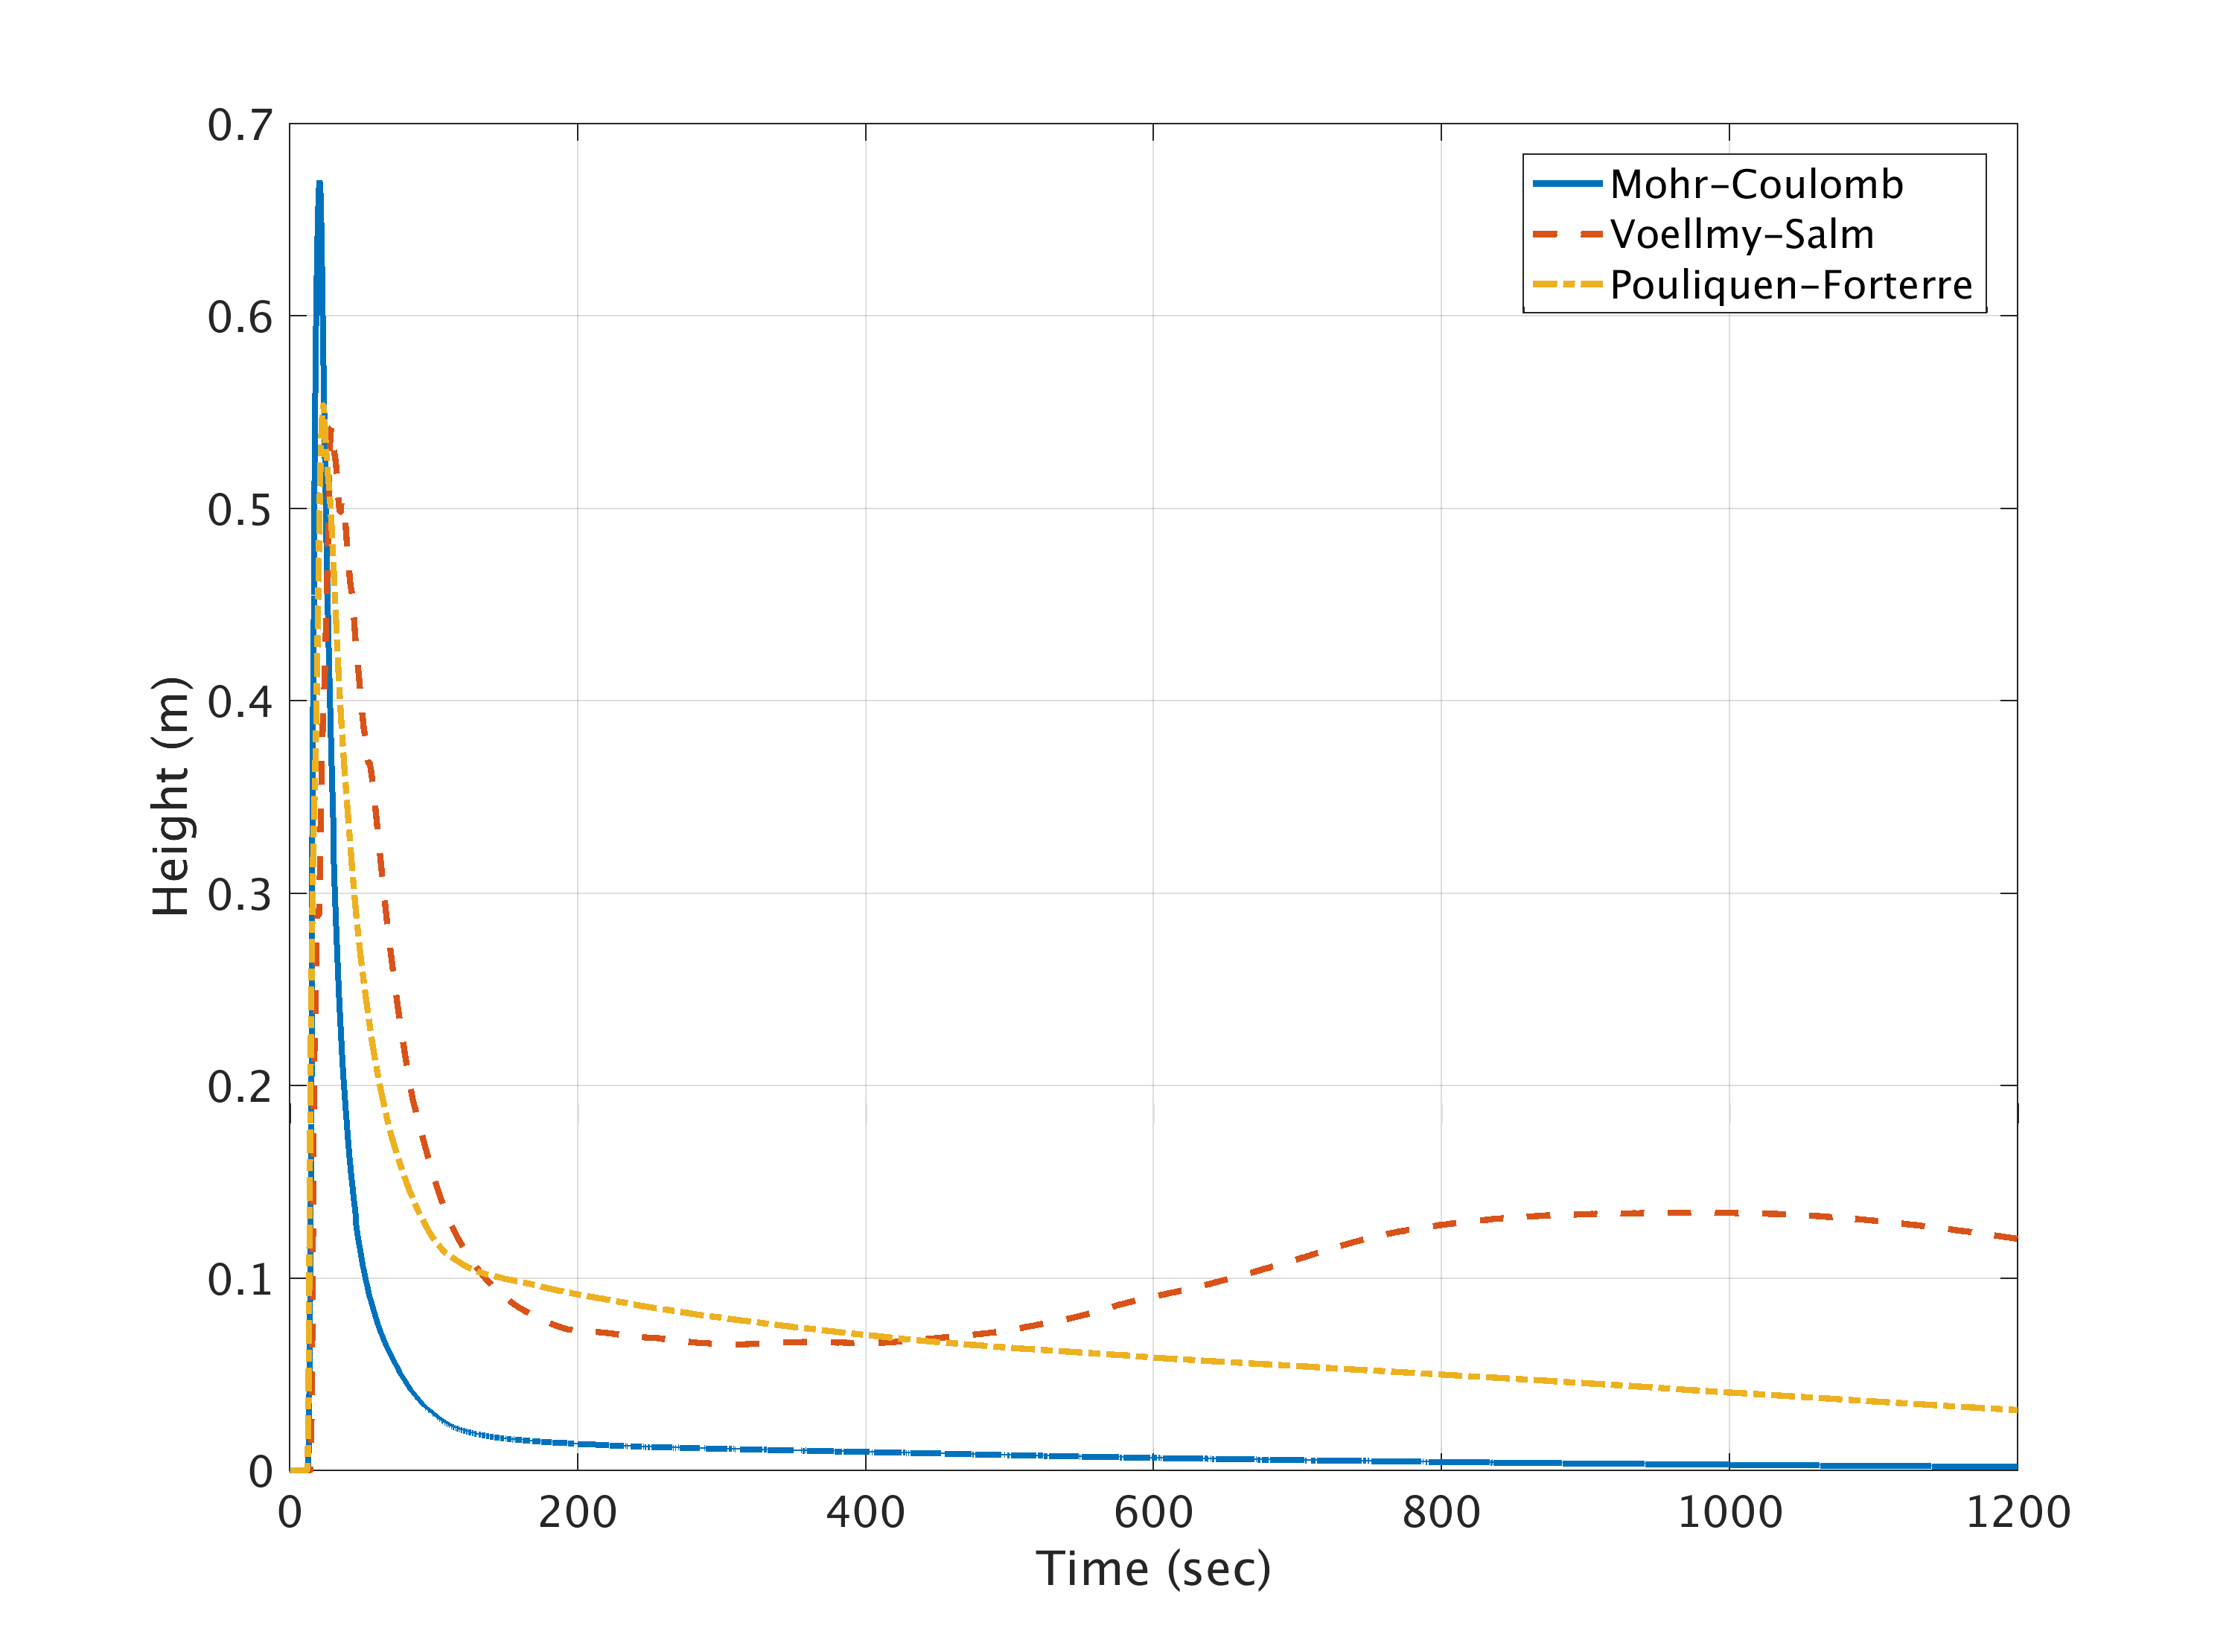
\includegraphics[width=1\textwidth]{HeightMeans/H3All.png}     
        \subcaption{Flow Height Records, Location 3.}
        \label{fig:MFHR_L3}
	\end{minipage}
	\begin{minipage}[b]{0.5\linewidth}
	\centering
    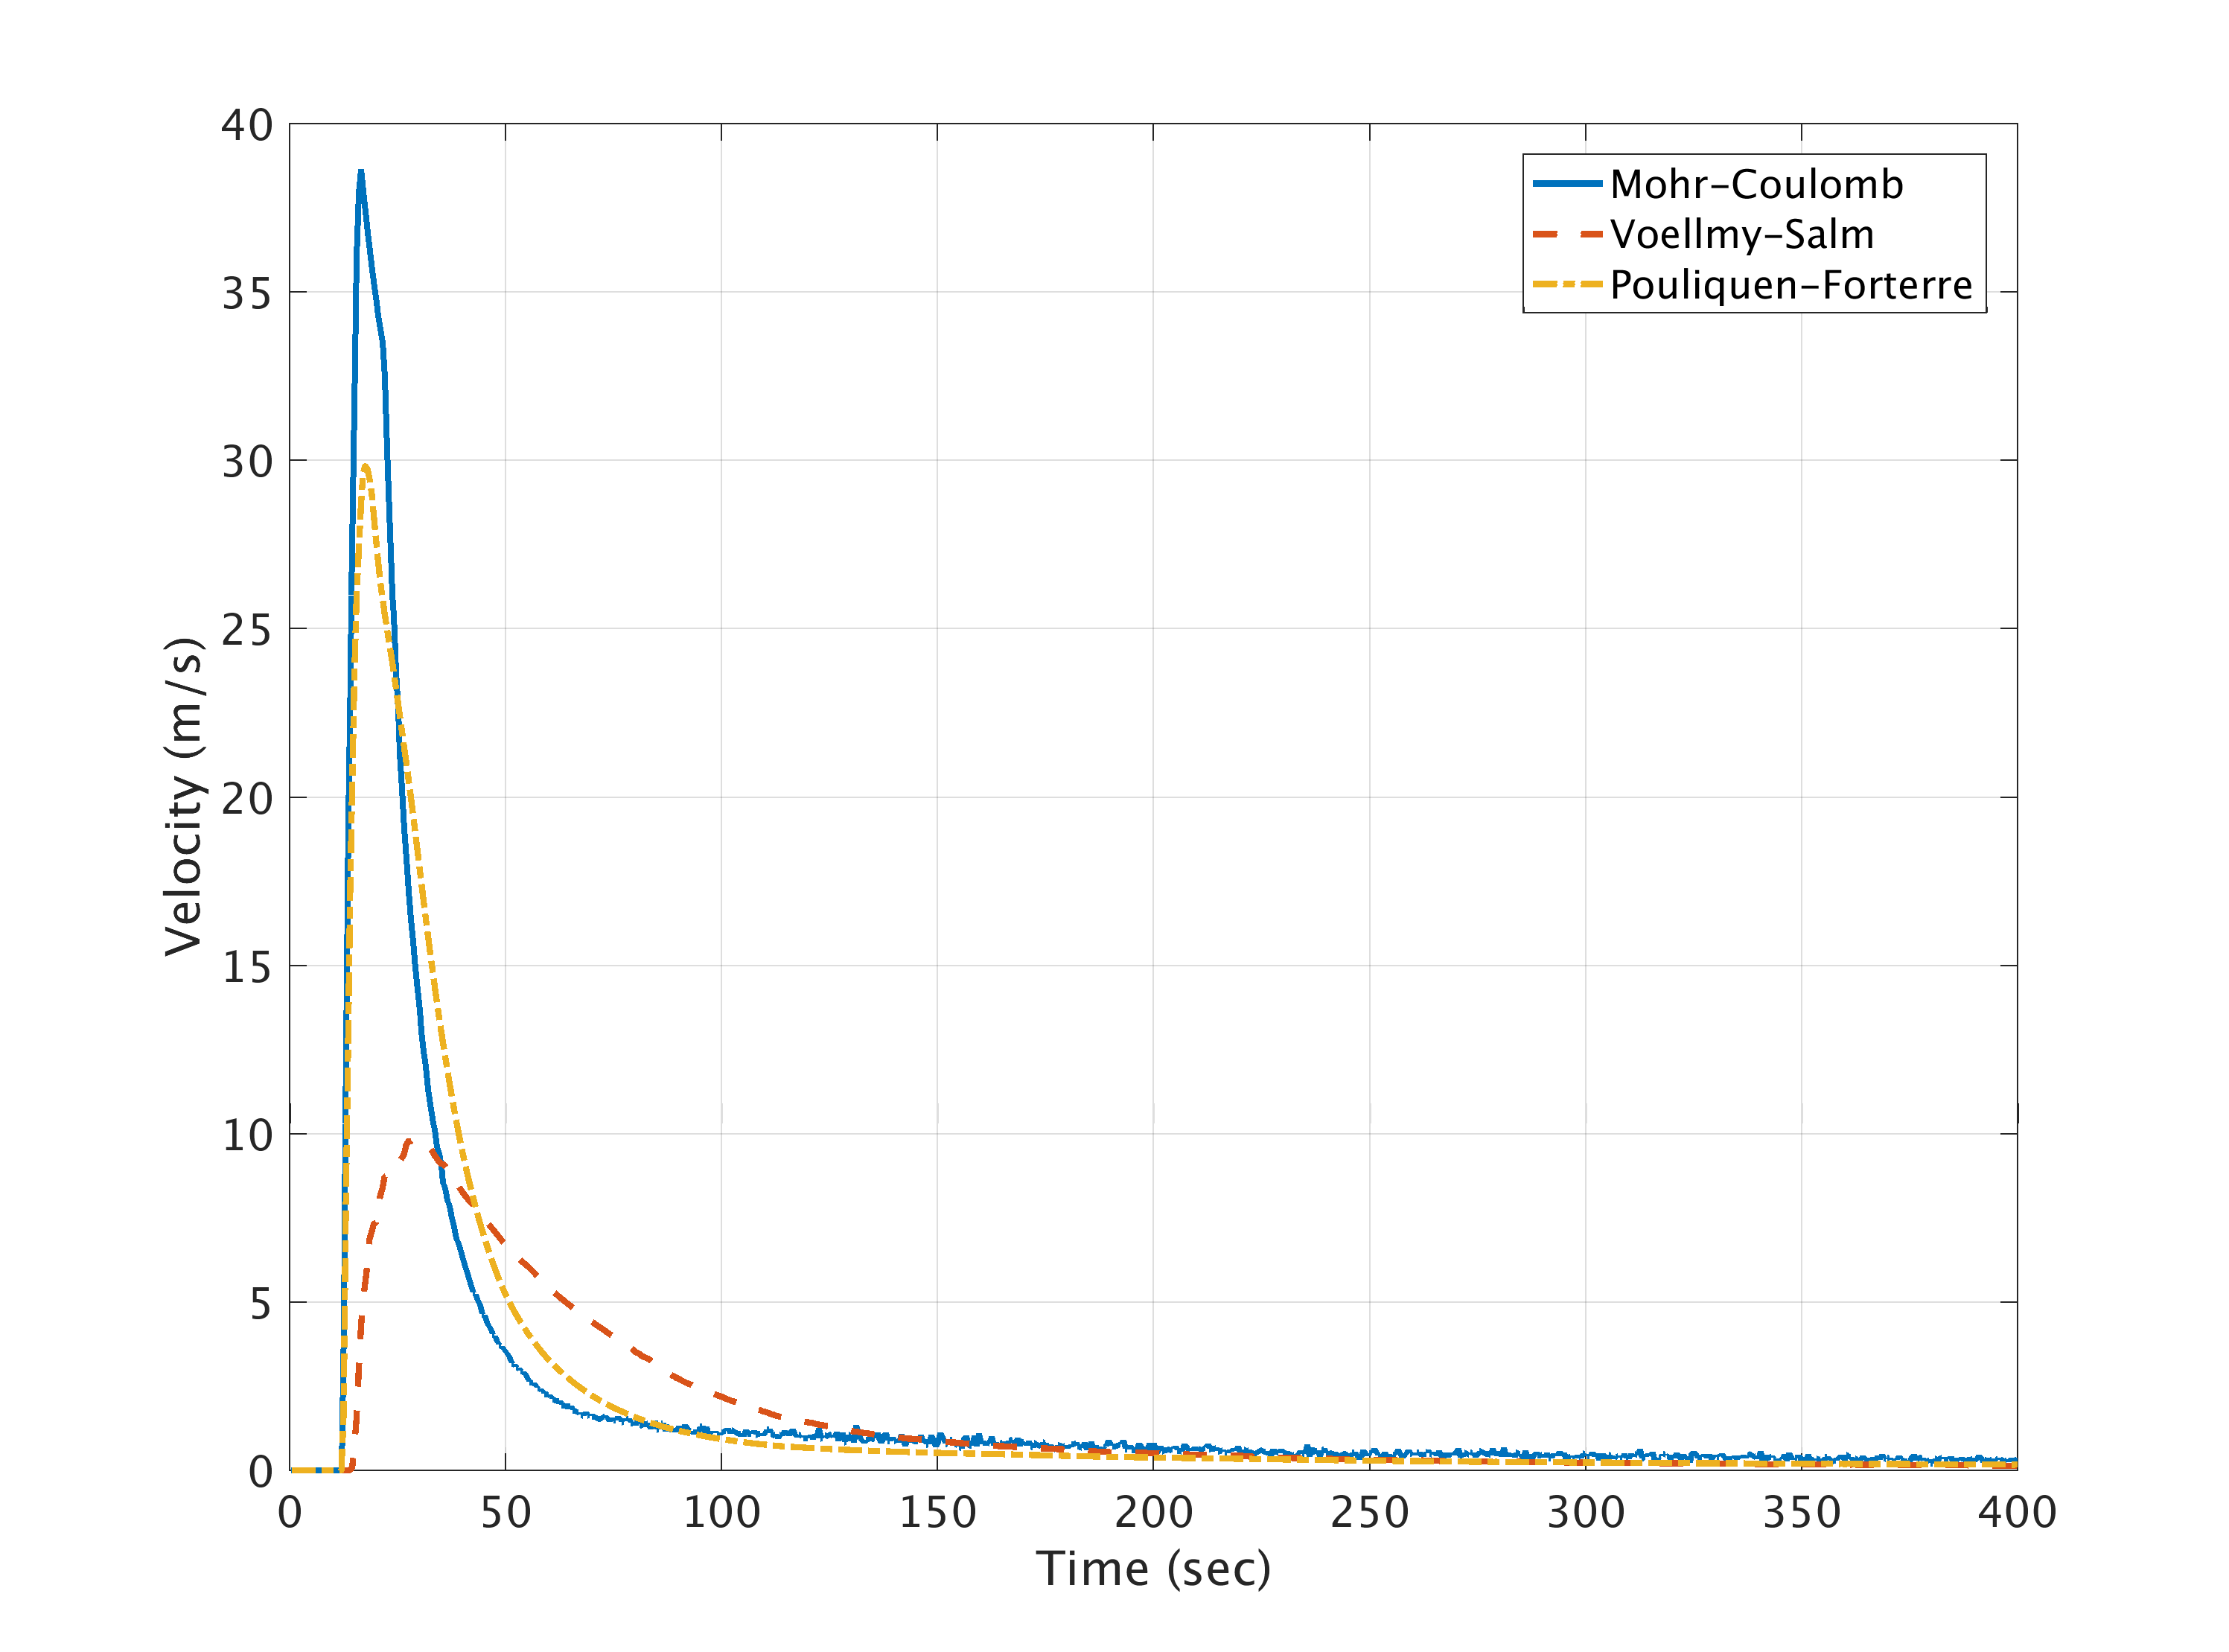
\includegraphics[width=1\textwidth]{VelocityMeans/V3All.png}
        \subcaption{Flow Velocity Records, Location 3.}
        \label{fig:MFVR_L3}
	\end{minipage}
	
	\caption{Mean Values of Flow Height and Velocity Records at locations 1,2 and 3.}\label{fig:MFHVR_L123}	
\end{figure}

\begin{figure}[H]
	\begin{minipage}[b]{0.5\linewidth}
	\centering
    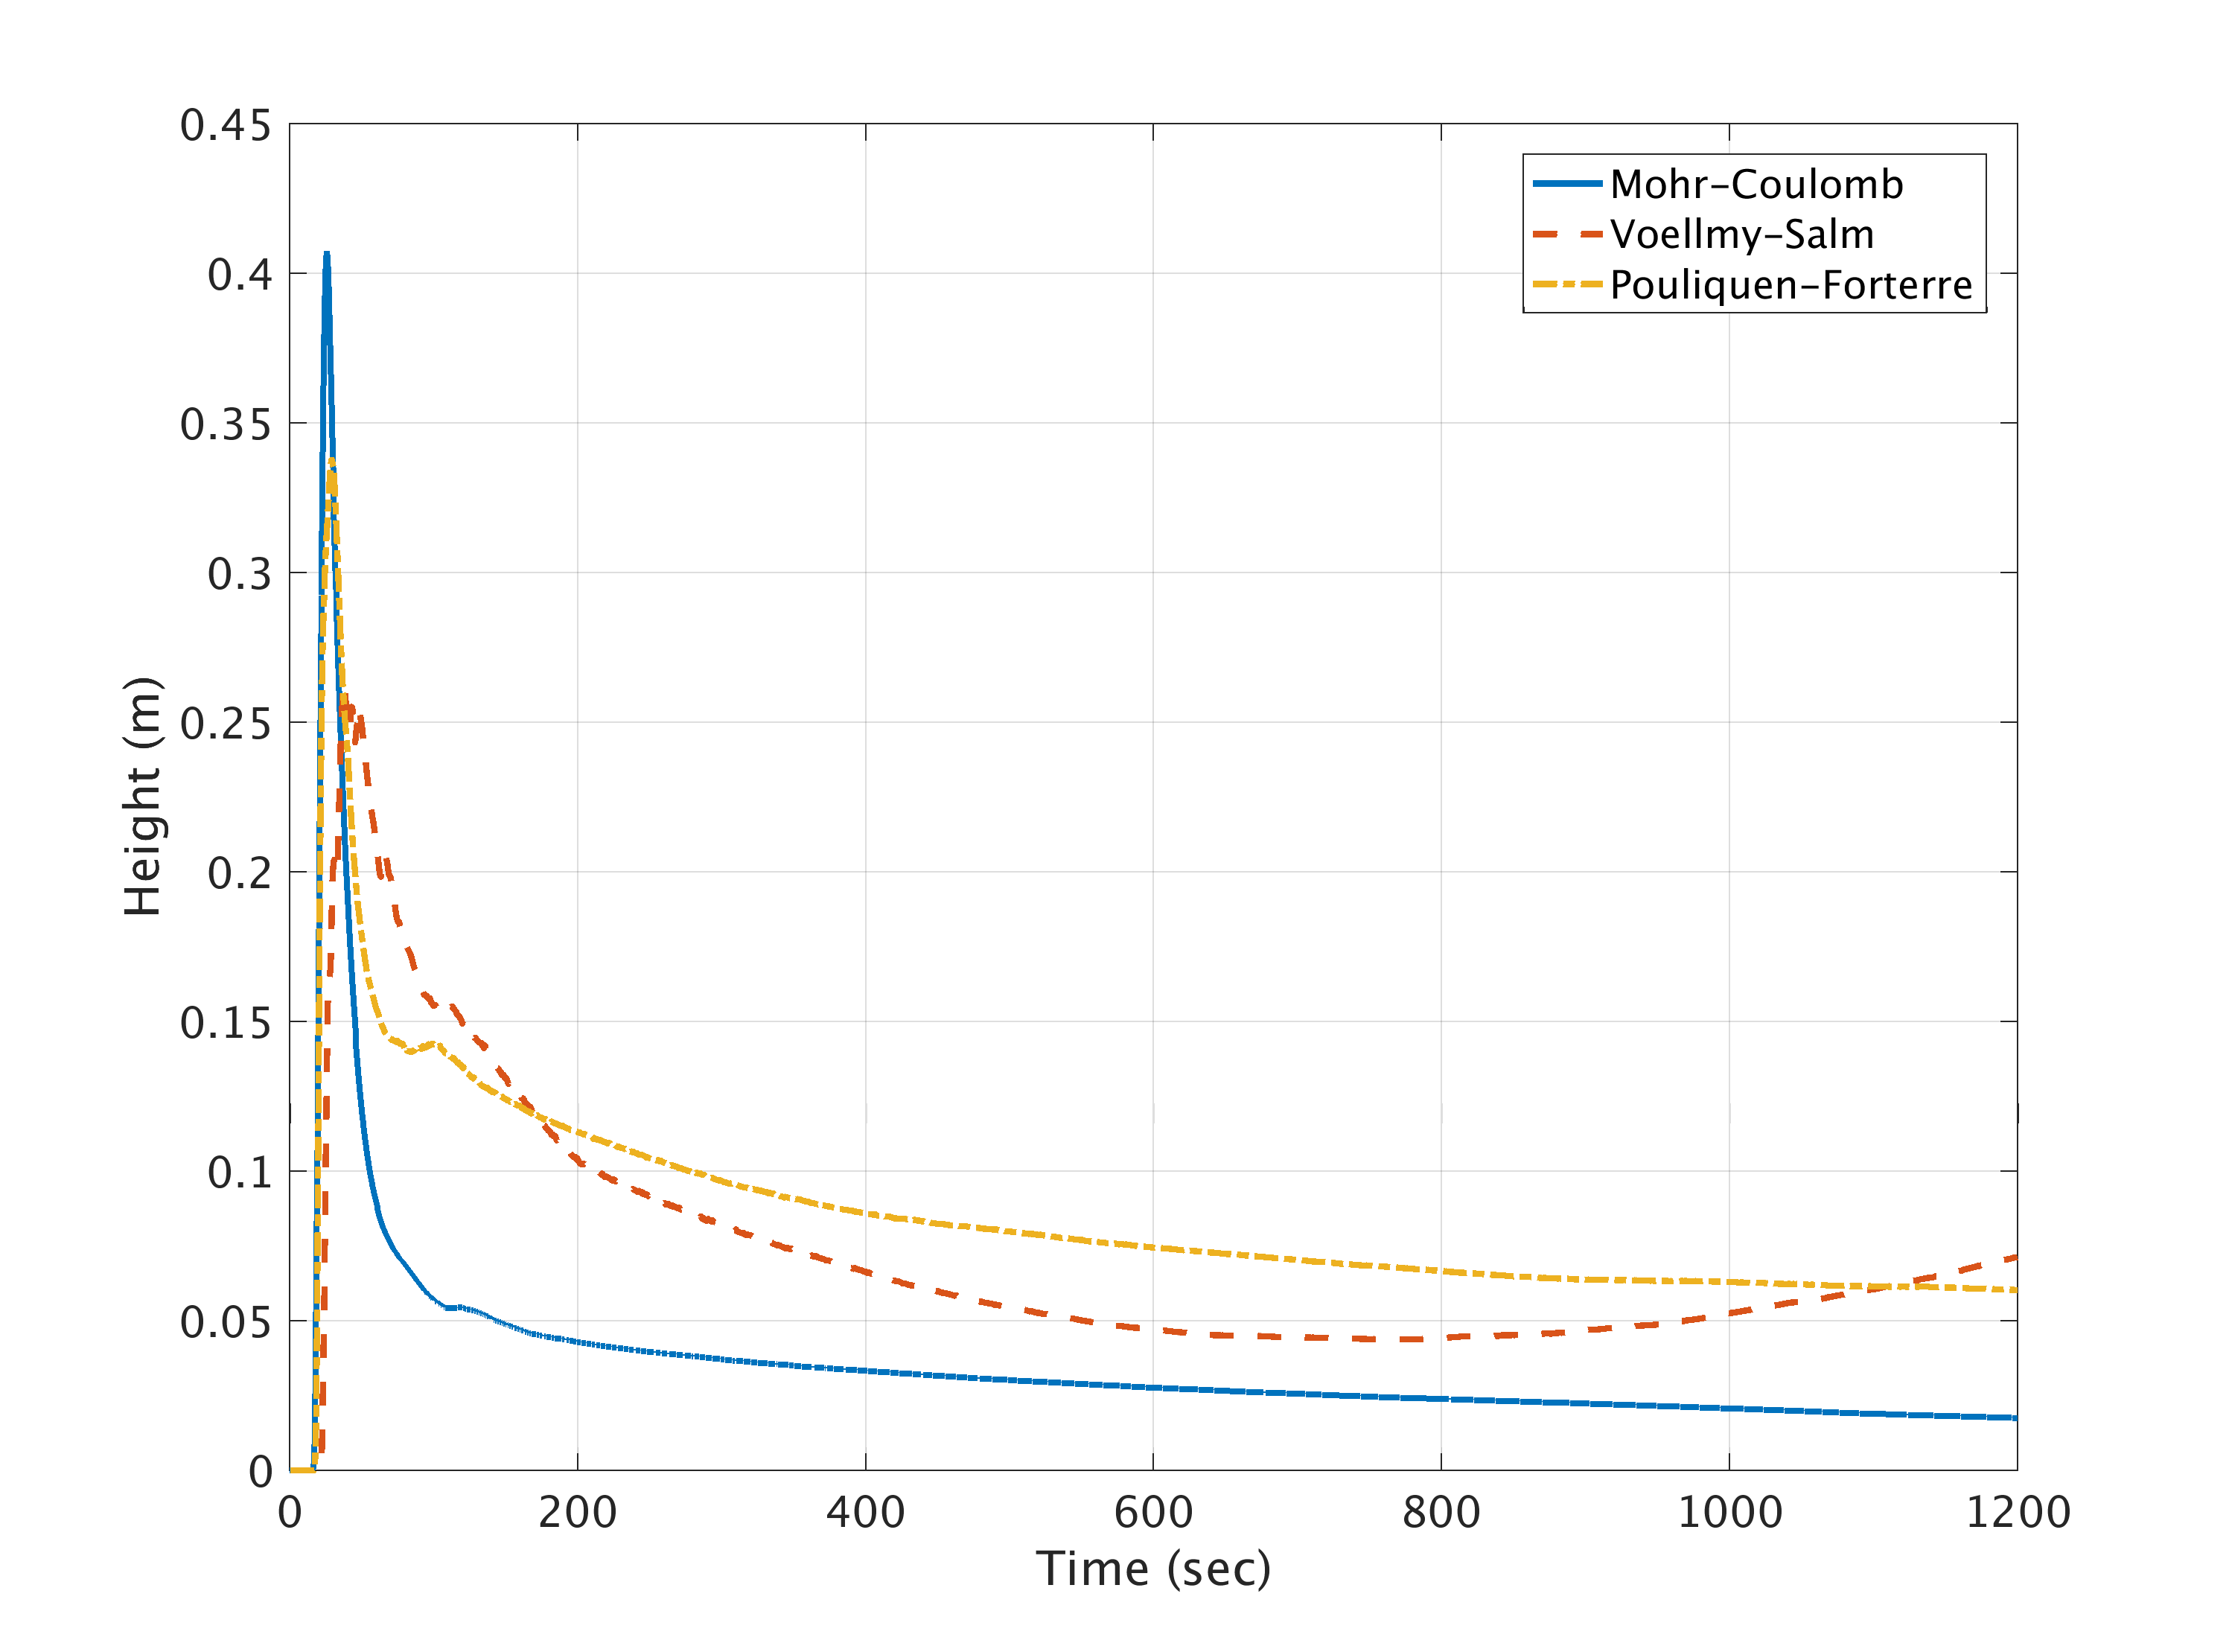
\includegraphics[width=1\textwidth]{HeightMeans/H4All.png}     
        \subcaption{Flow Height Records, Location 4.}
        \label{fig:MFHR_L4}
	\end{minipage}
	\begin{minipage}[b]{0.5\linewidth}
	\centering
    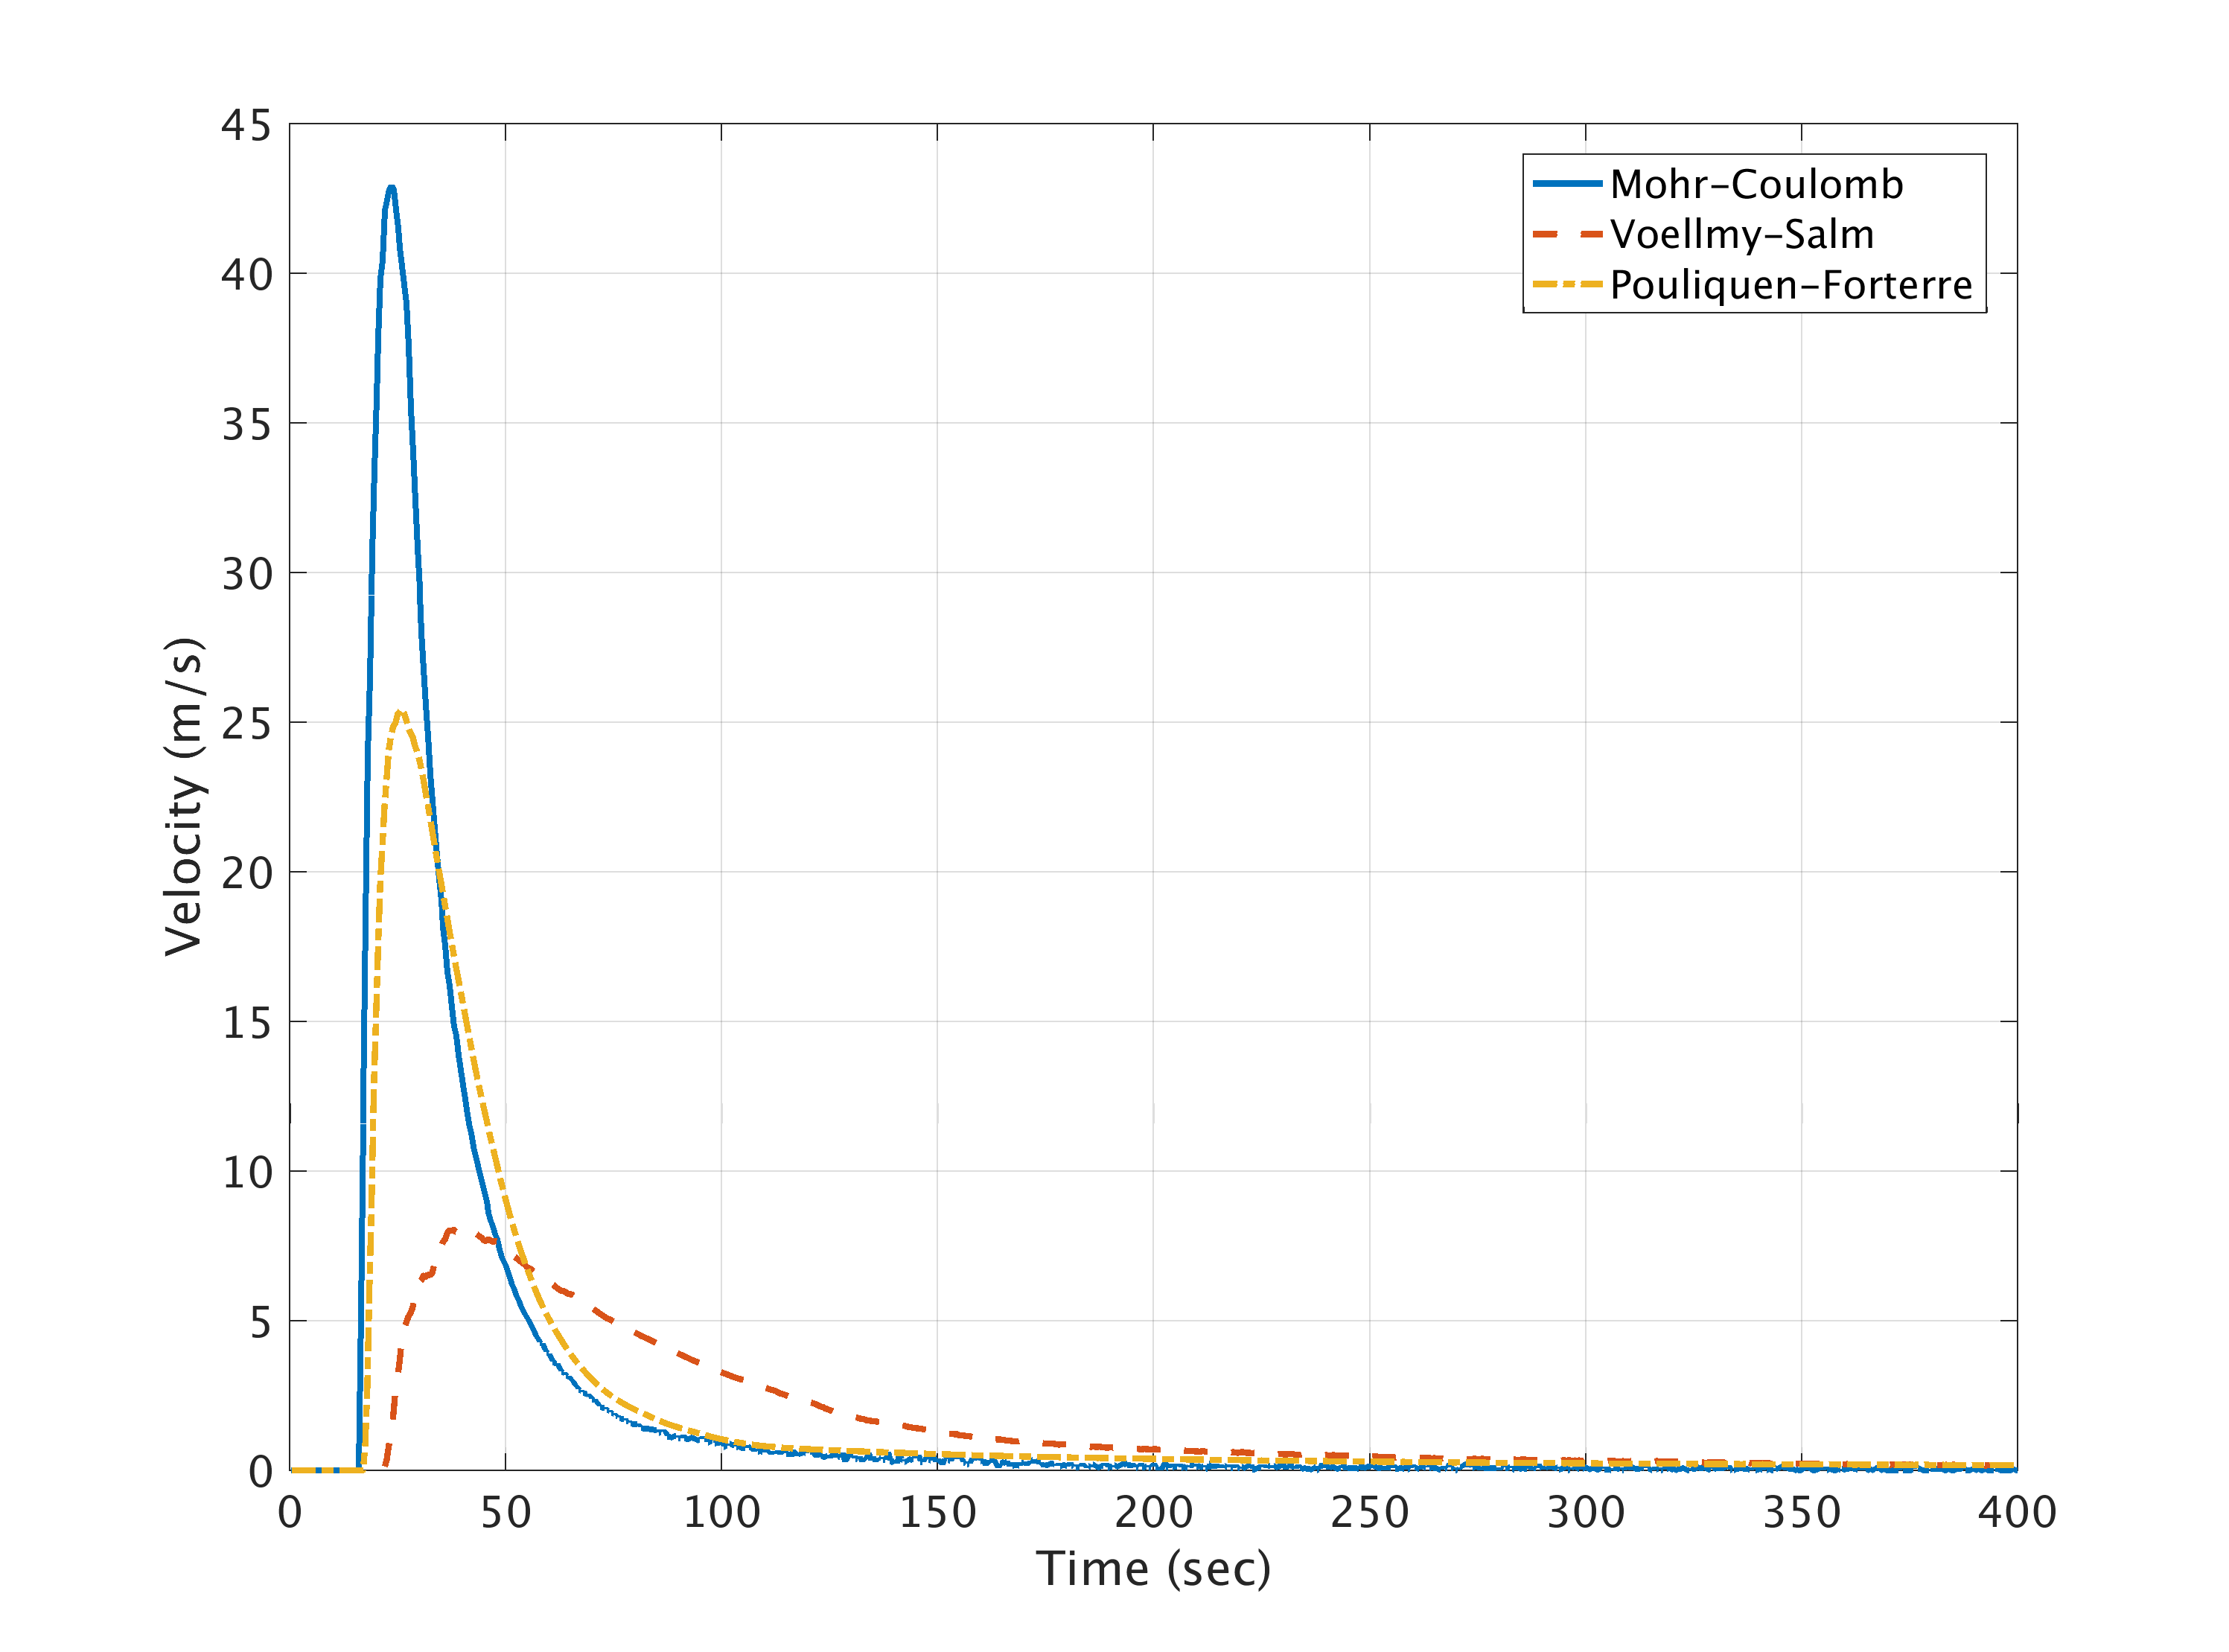
\includegraphics[width=1\textwidth]{VelocityMeans/V4All.png}
        \subcaption{Flow Velocity Records, Location 4.}
        \label{fig:MFVR_L4}
	\end{minipage}
	
	\begin{minipage}[b]{0.5\linewidth}
	\centering
    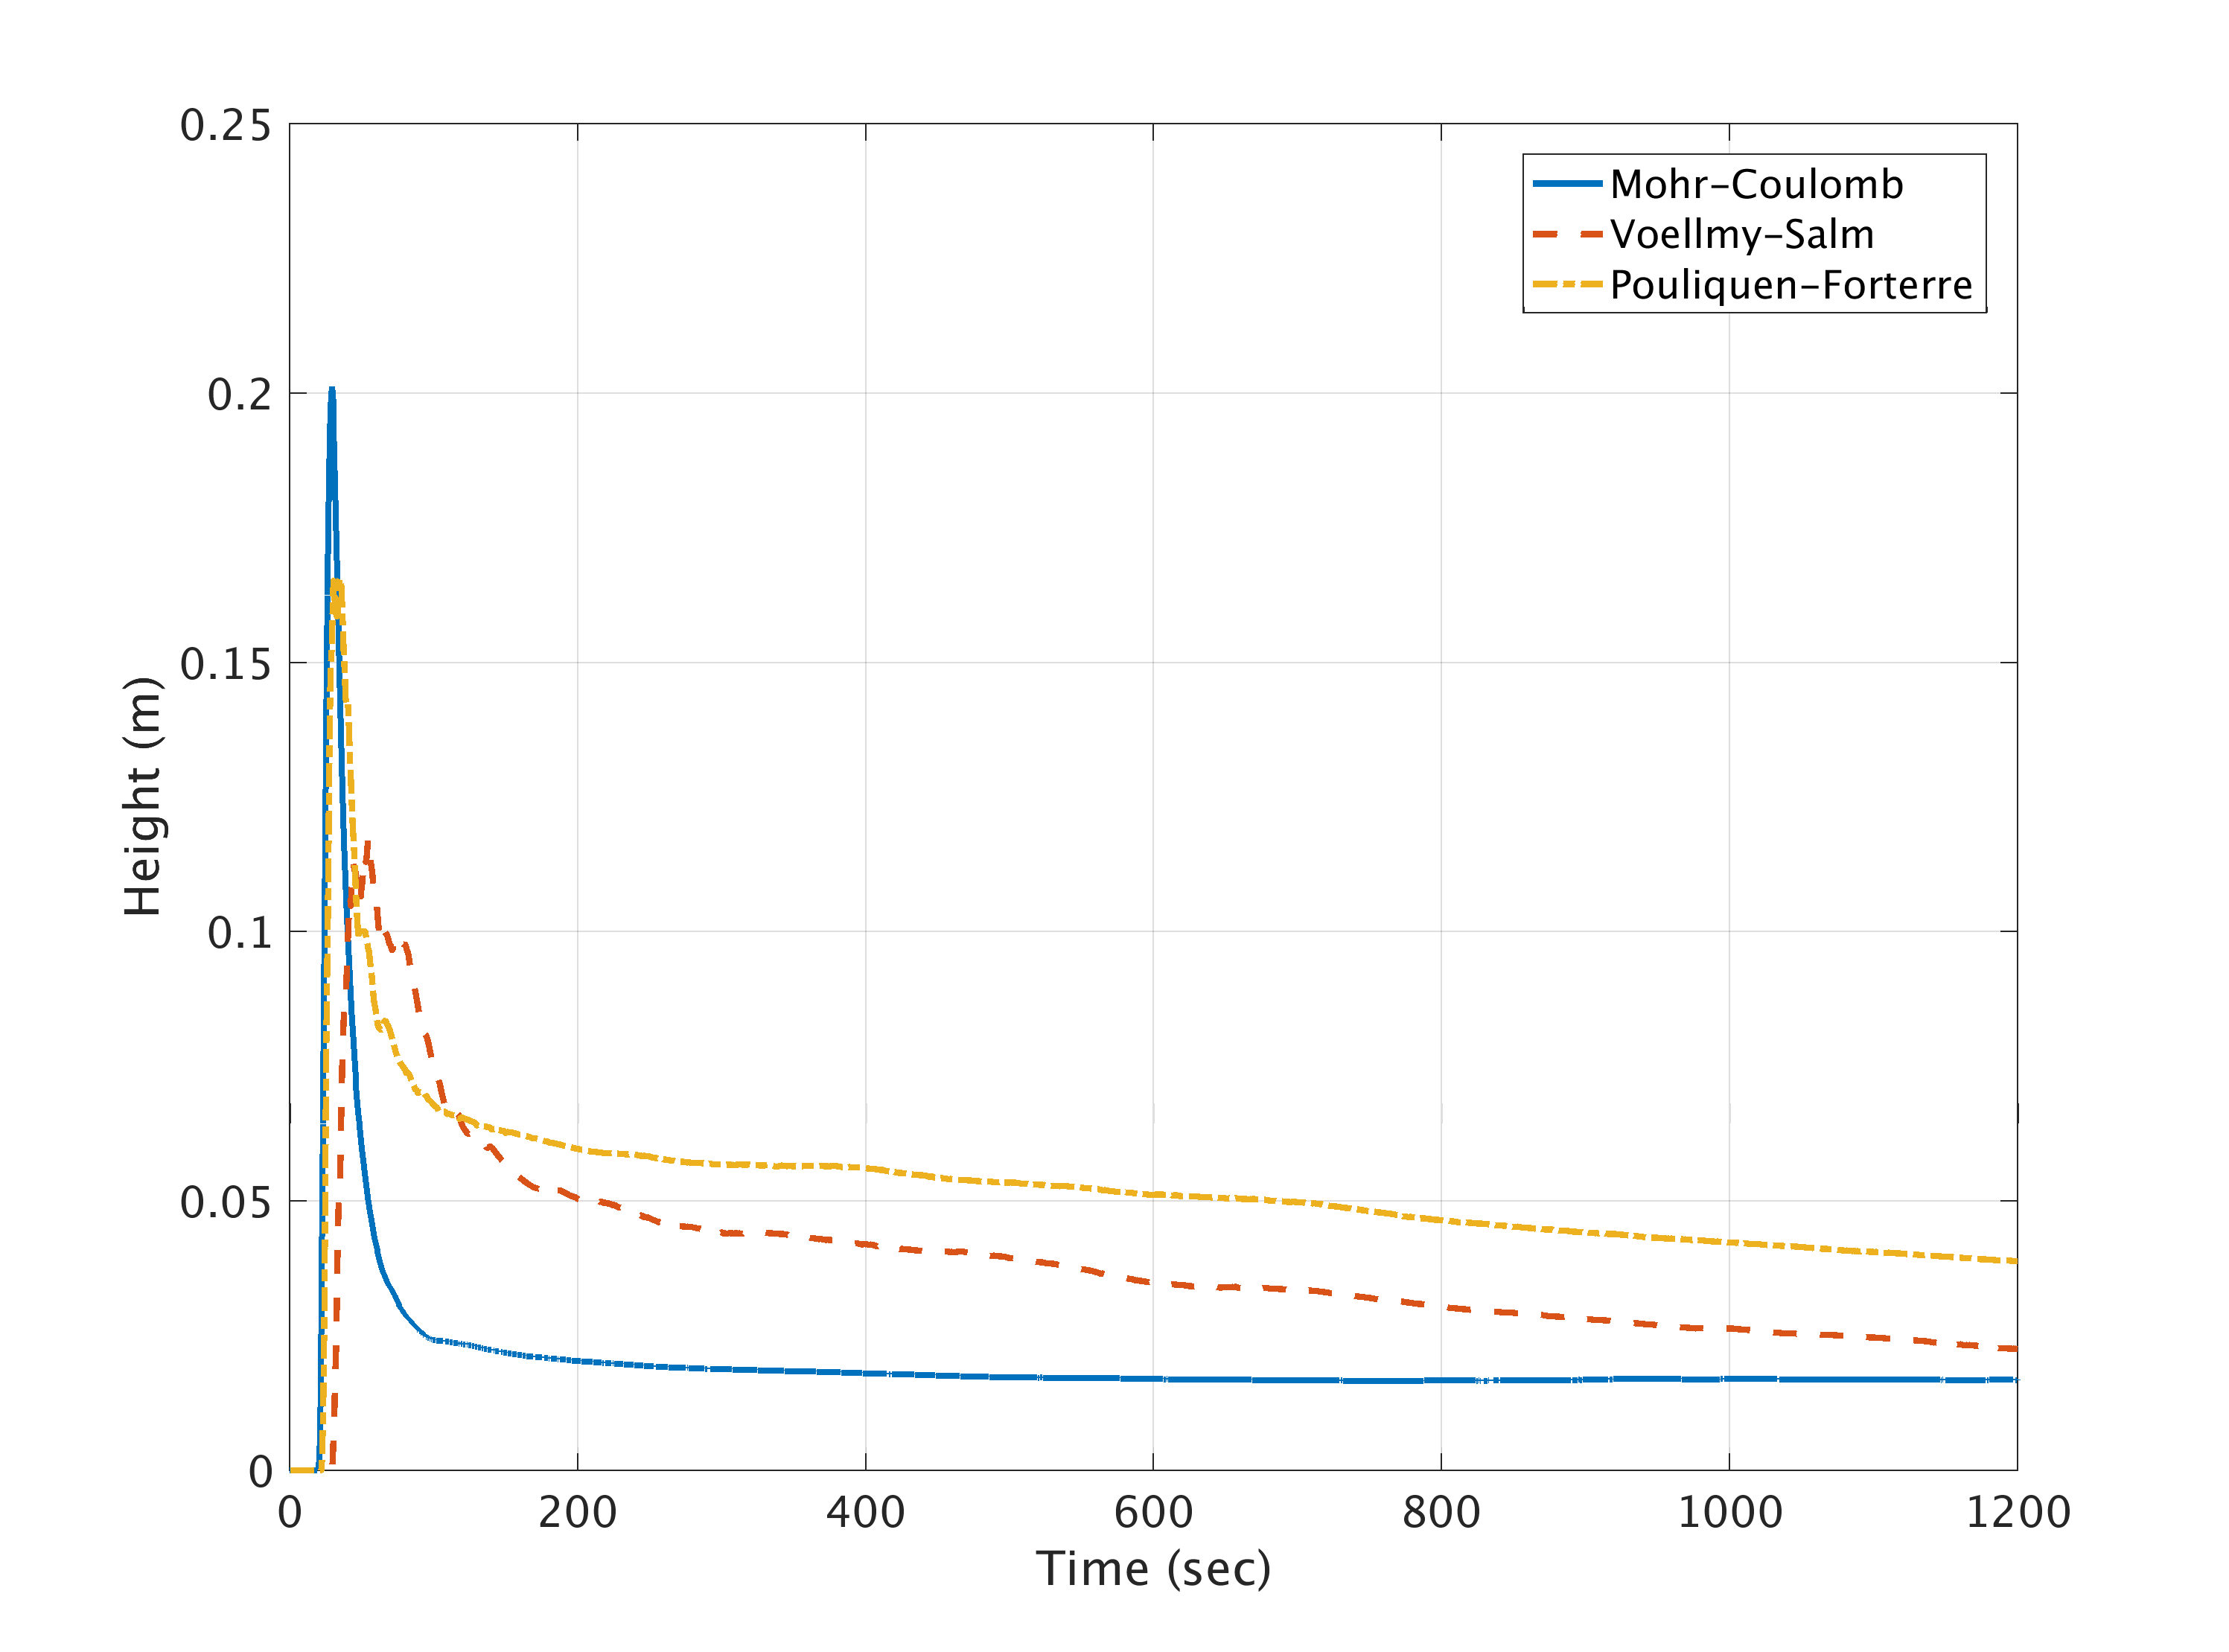
\includegraphics[width=1\textwidth]{HeightMeans/H5All.png}     
        \subcaption{Flow Height Records, Location 5.}
        \label{fig:MFHR_L5}
	\end{minipage}
	\begin{minipage}[b]{0.5\linewidth}
	\centering
    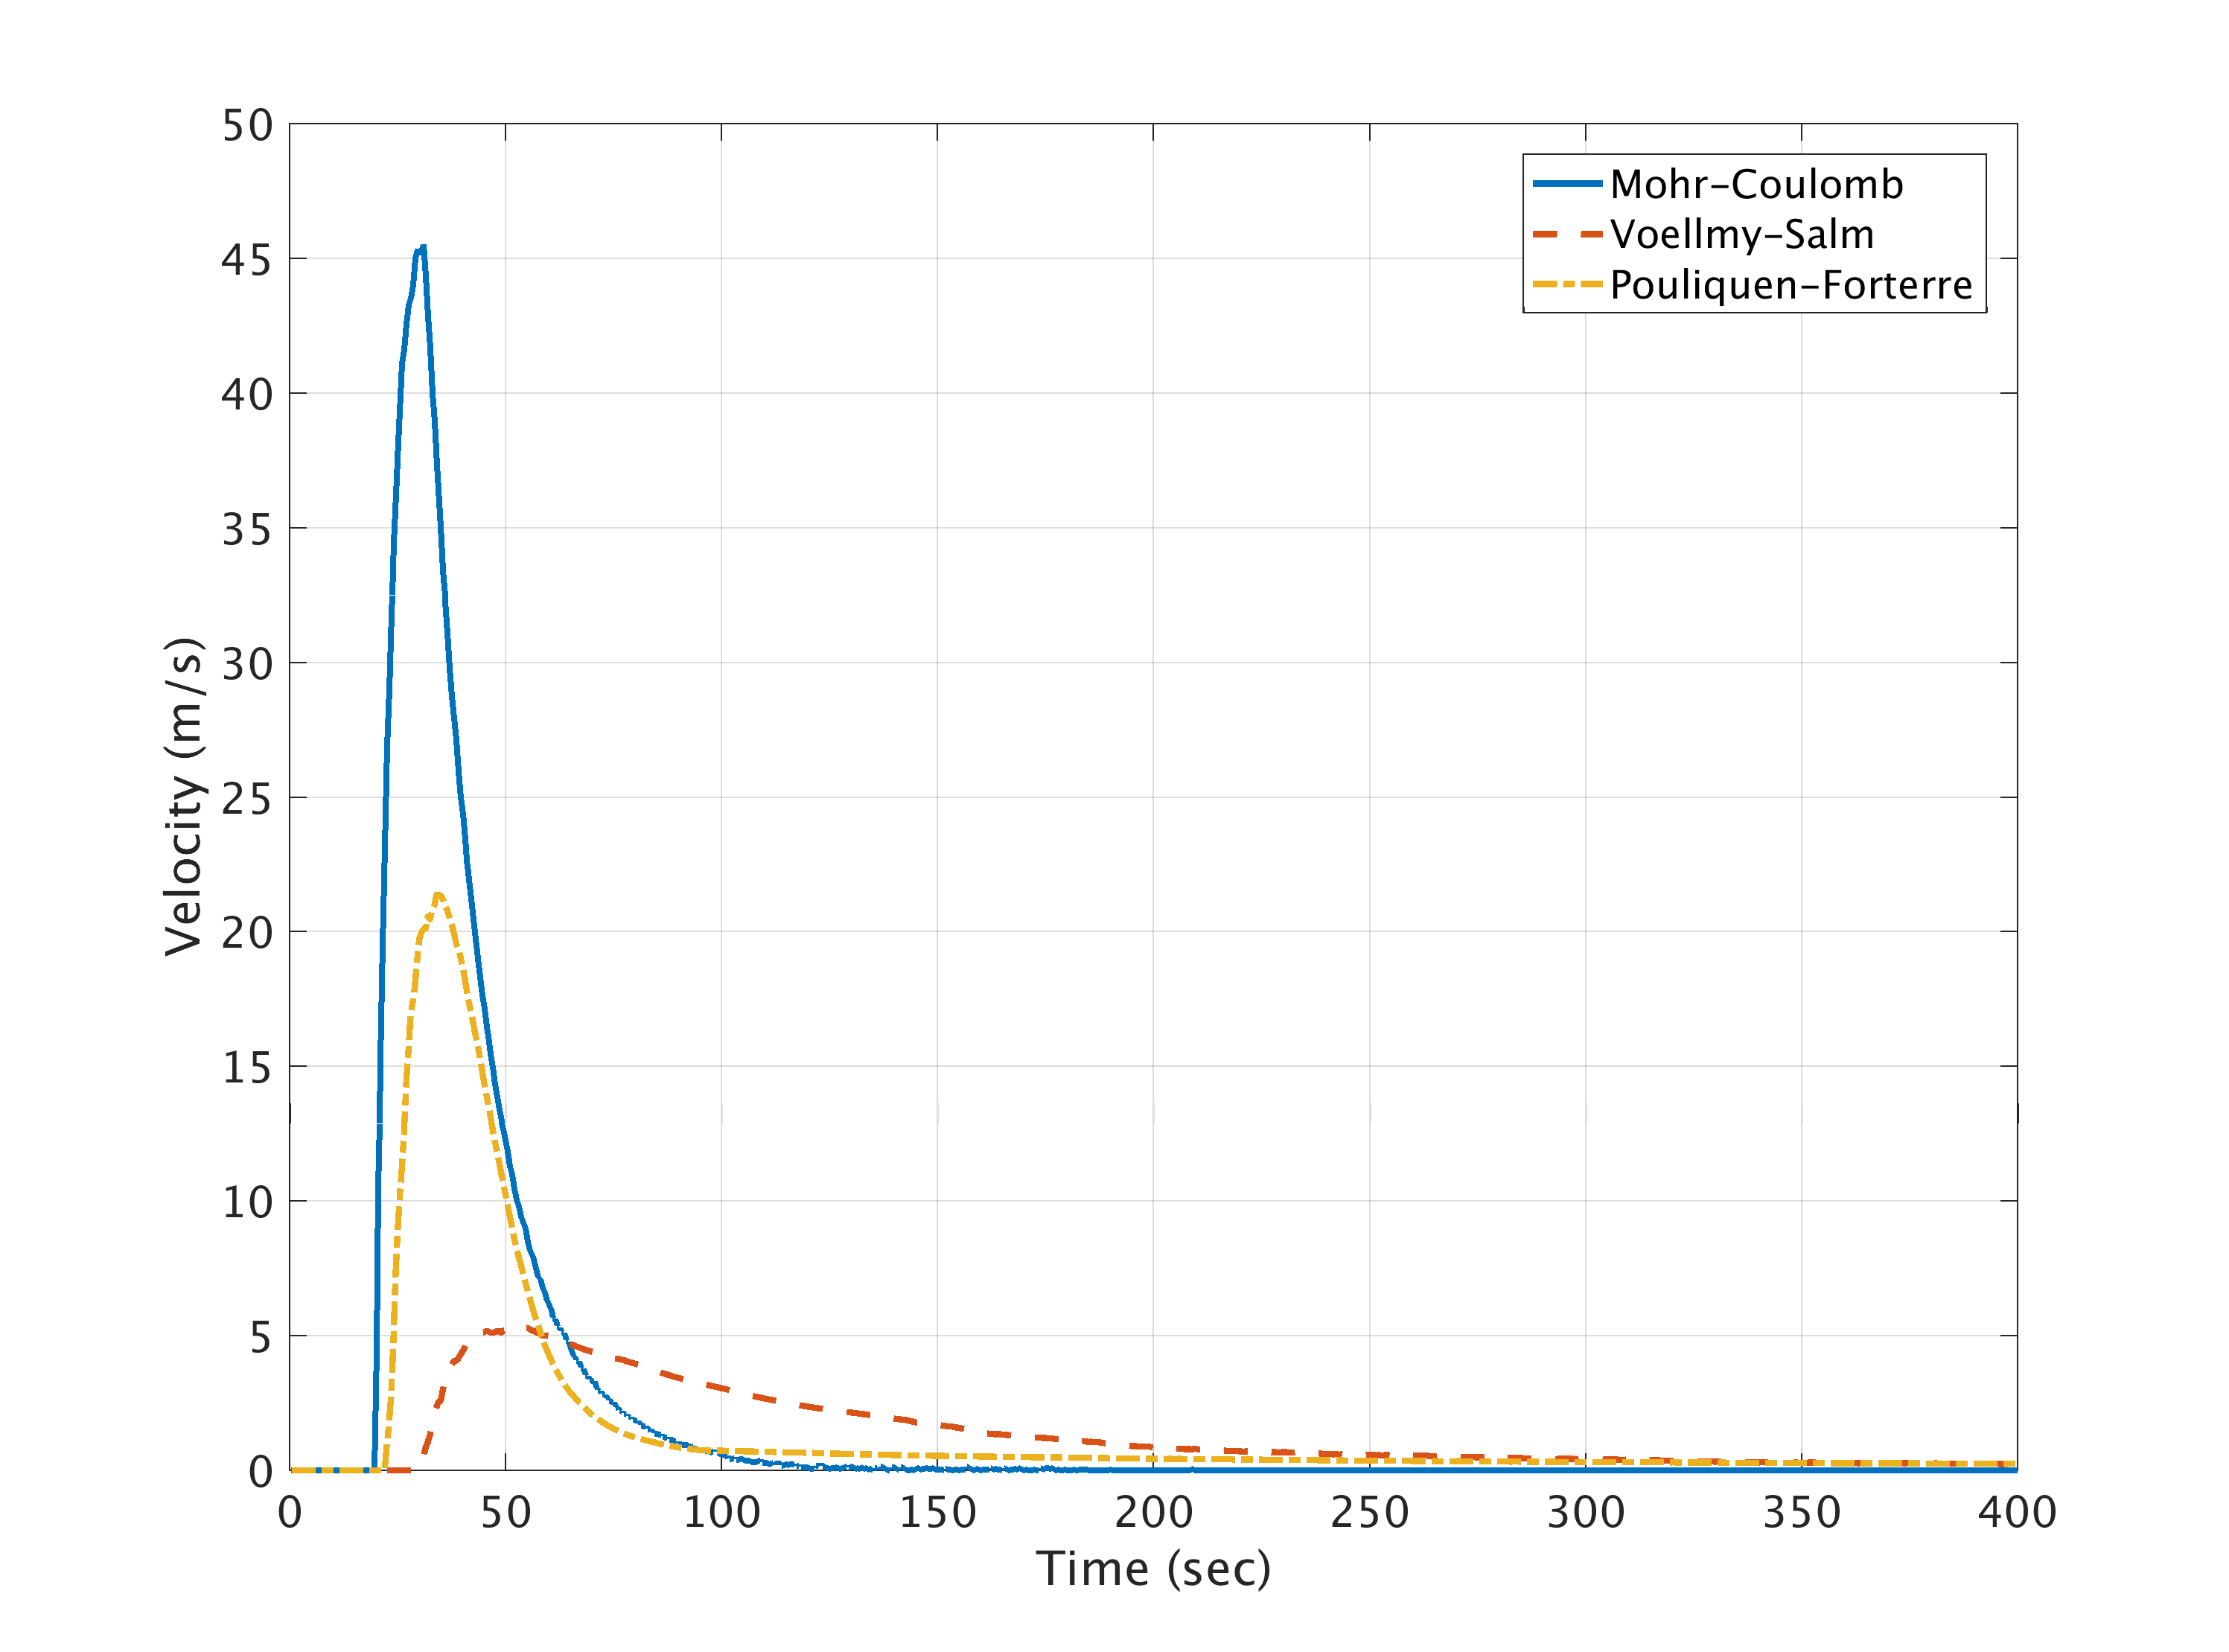
\includegraphics[width=1\textwidth]{VelocityMeans/V5All.png}
        \subcaption{Flow Velocity Records, Location 5.}
        \label{fig:MFVR_L5}
	\end{minipage}
	
	\begin{minipage}[b]{0.5\linewidth}
	\centering
    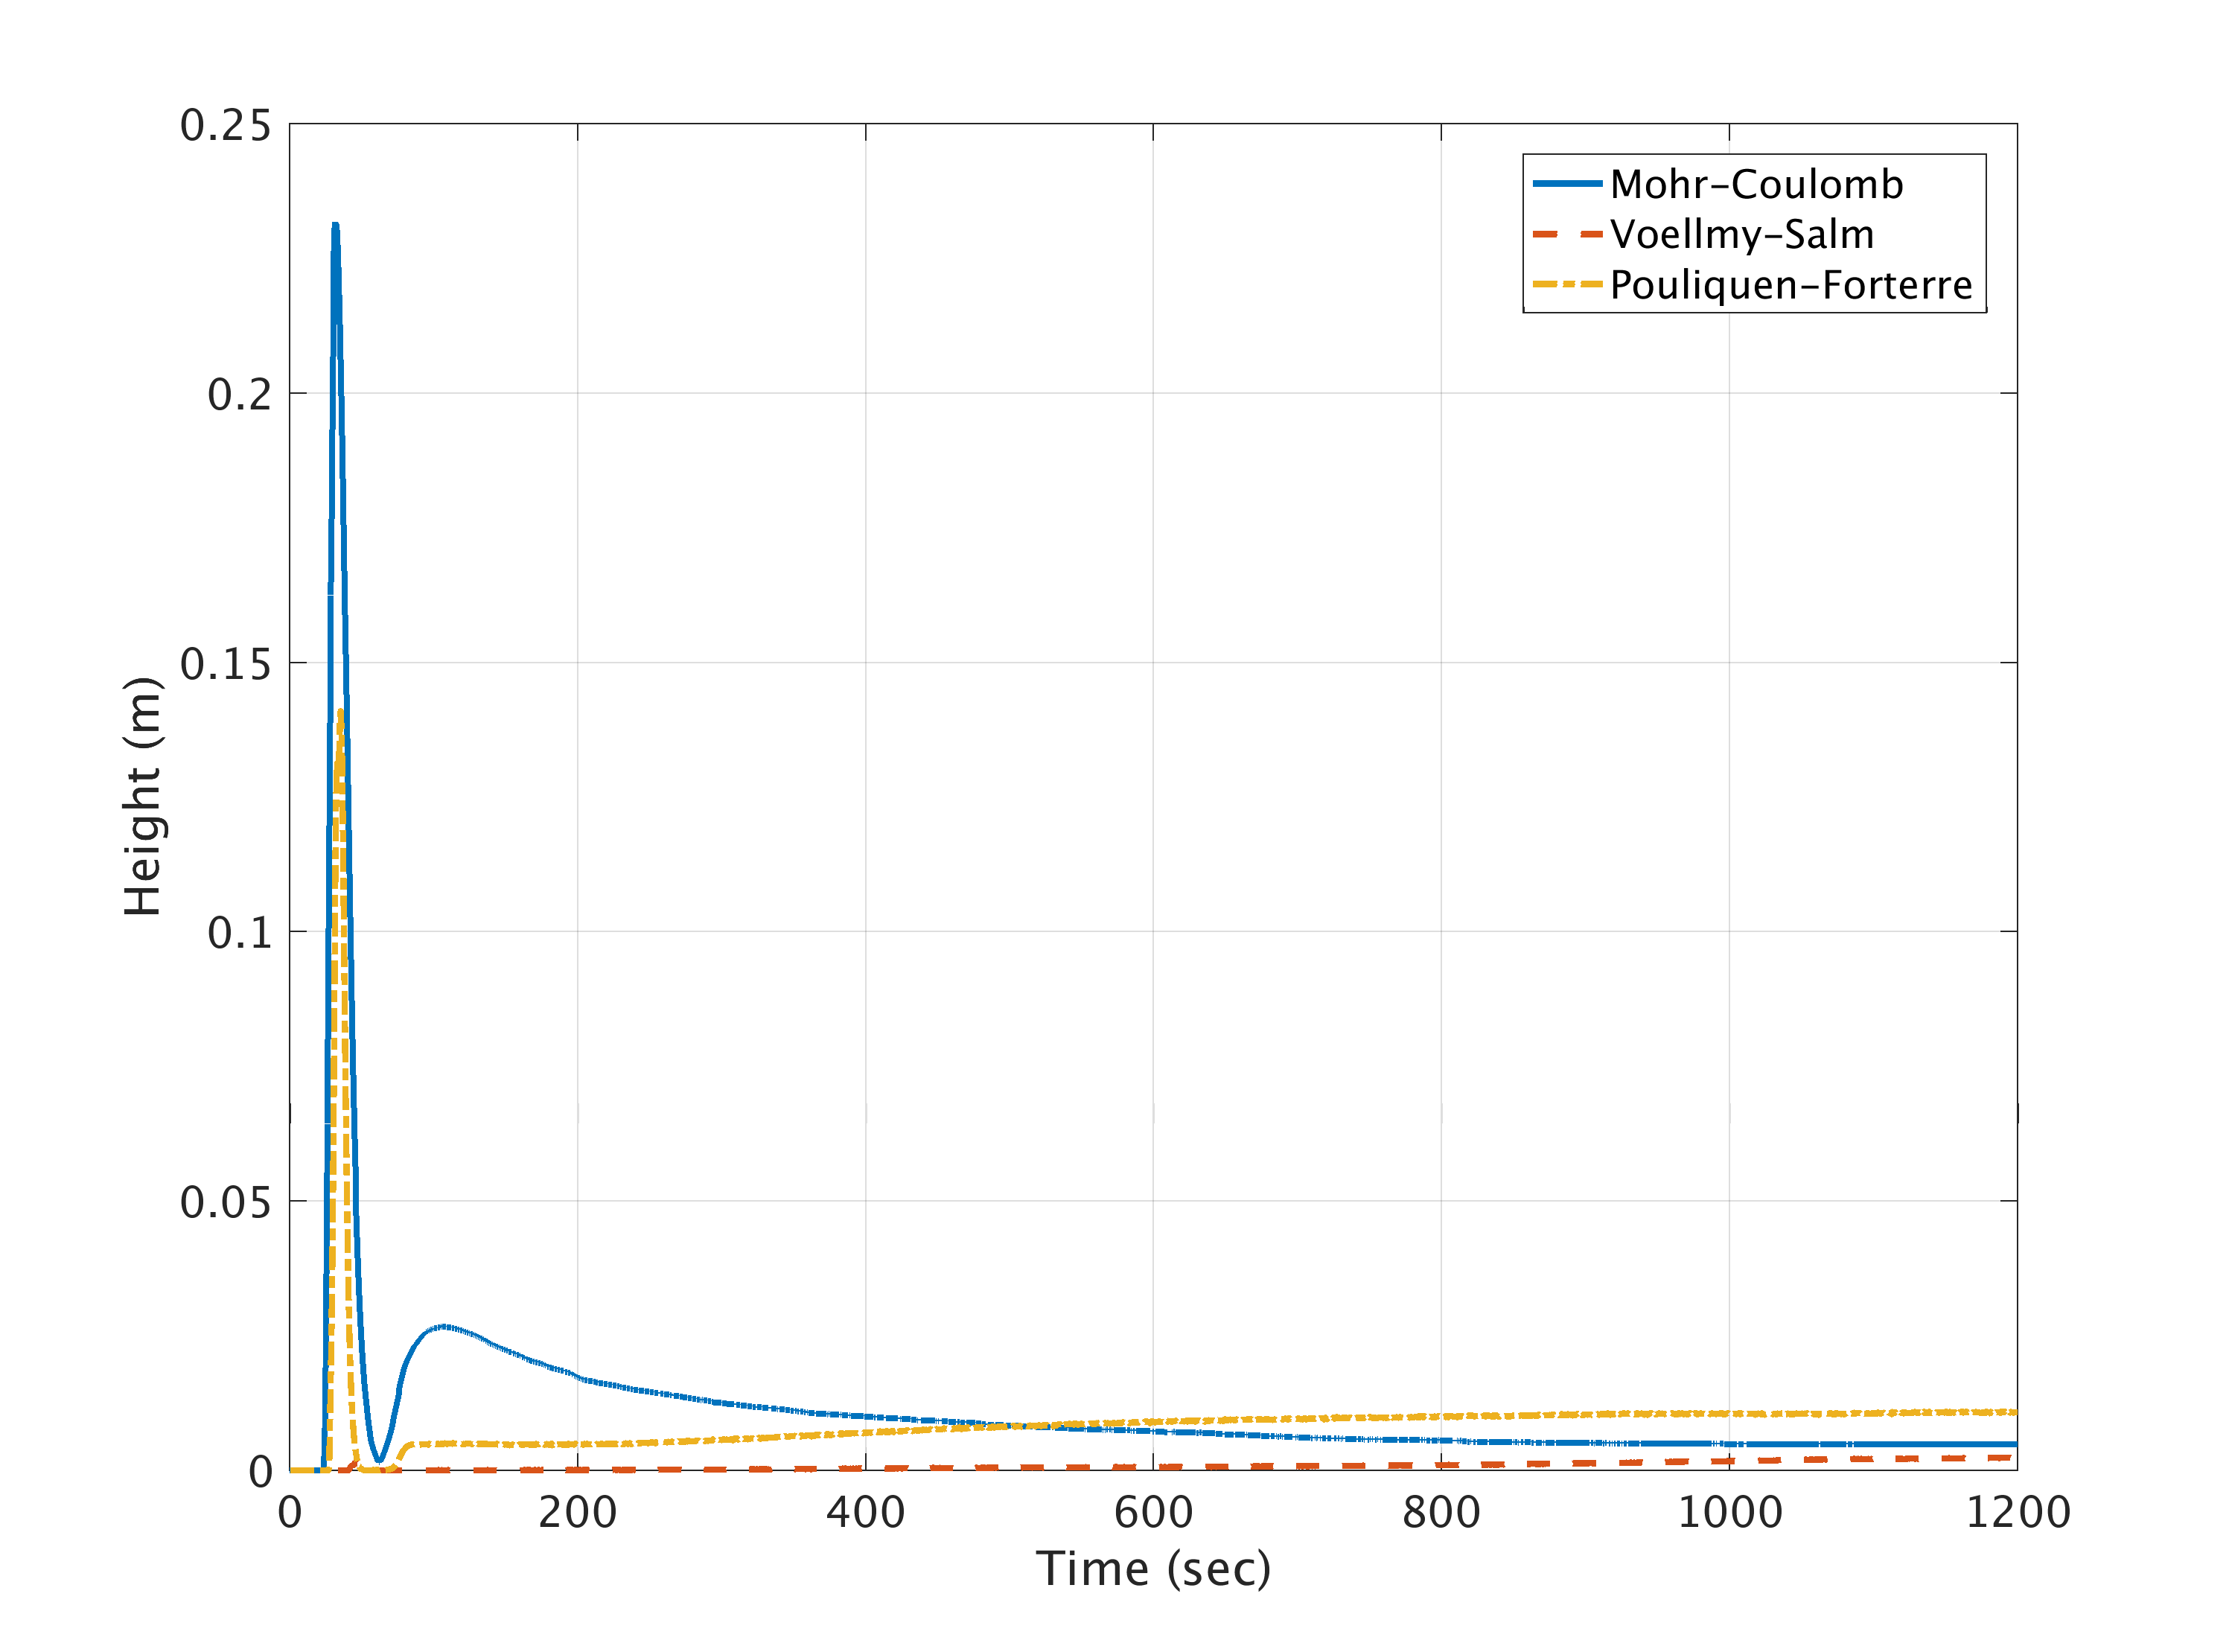
\includegraphics[width=1\textwidth]{HeightMeans/H6All.png}     
        \subcaption{Flow Height Records, Location 6.}
        \label{fig:MFHR_L6}
	\end{minipage}
	\begin{minipage}[b]{0.5\linewidth}
	\centering
    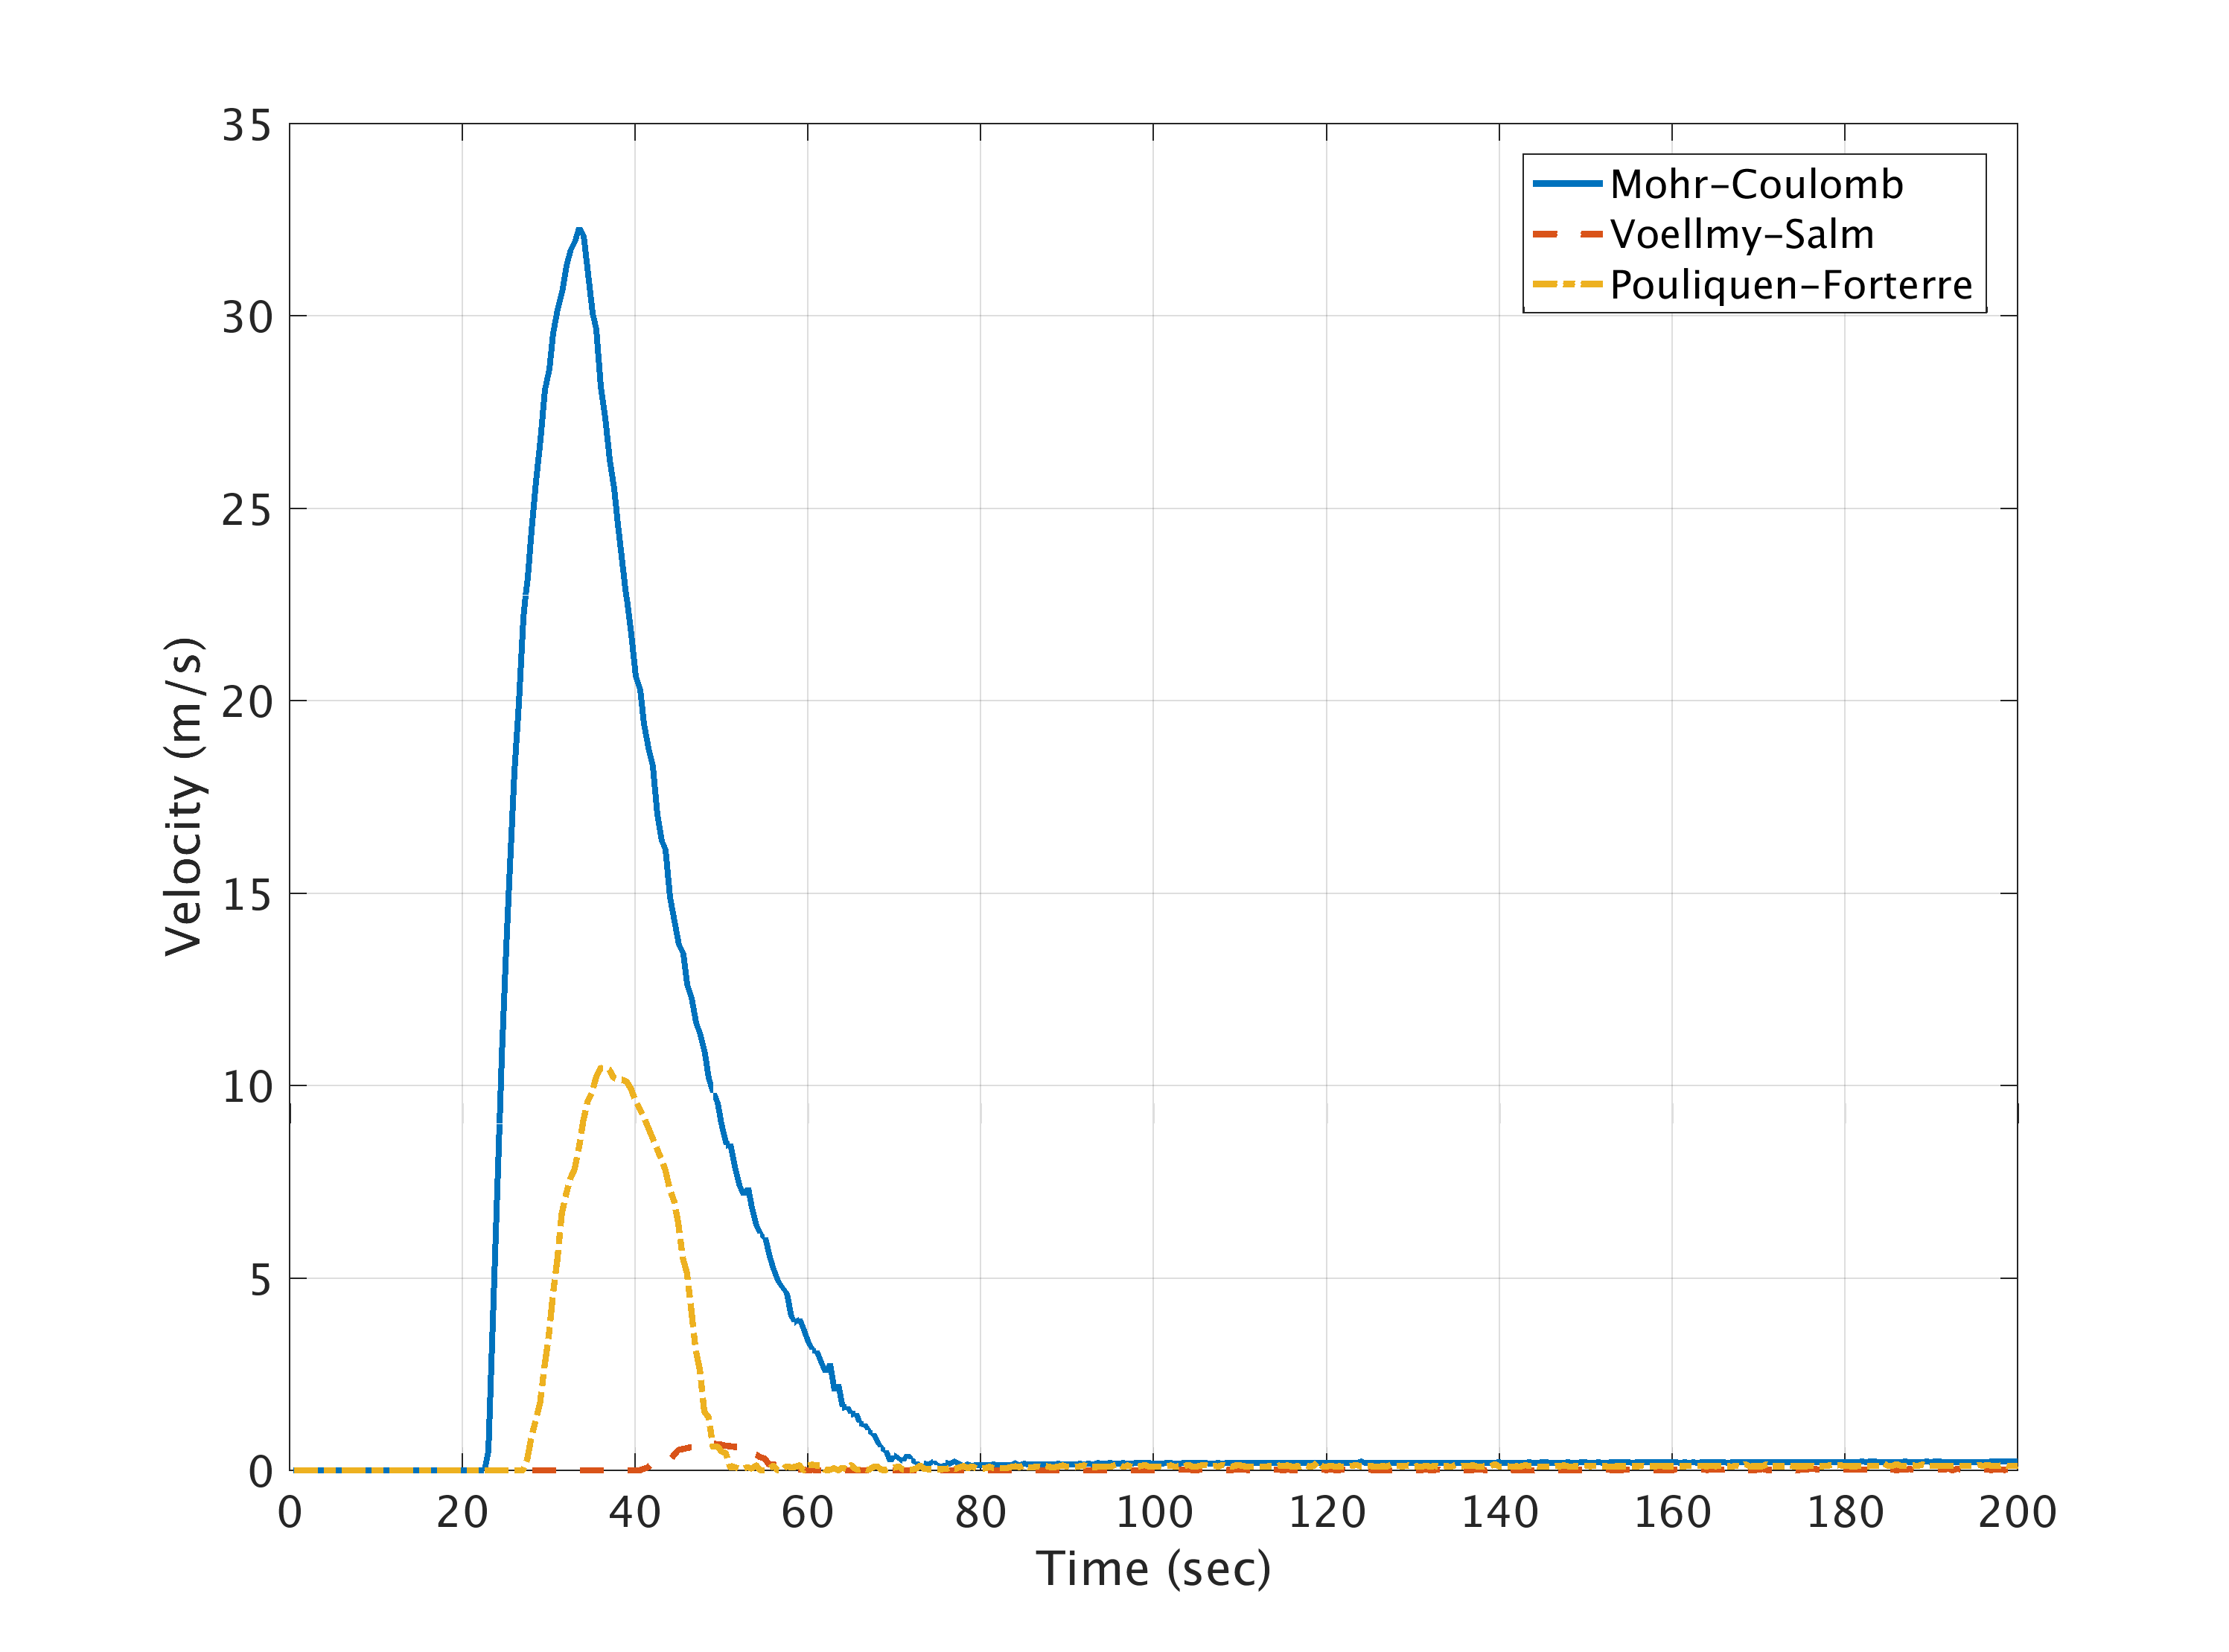
\includegraphics[width=1\textwidth]{VelocityMeans/V6All.png}
        \subcaption{Flow Velocity Records, Location 6.}
        \label{fig:MFVR_L6}
	\end{minipage}
		
	\caption{Mean Values of Flow Height and Velocity Records at locations 4,5 and 6.}\label{fig:MFHVR_L456}	
\end{figure}

\begin{figure}[H]
	\begin{minipage}[b]{0.5\linewidth}
	\centering
    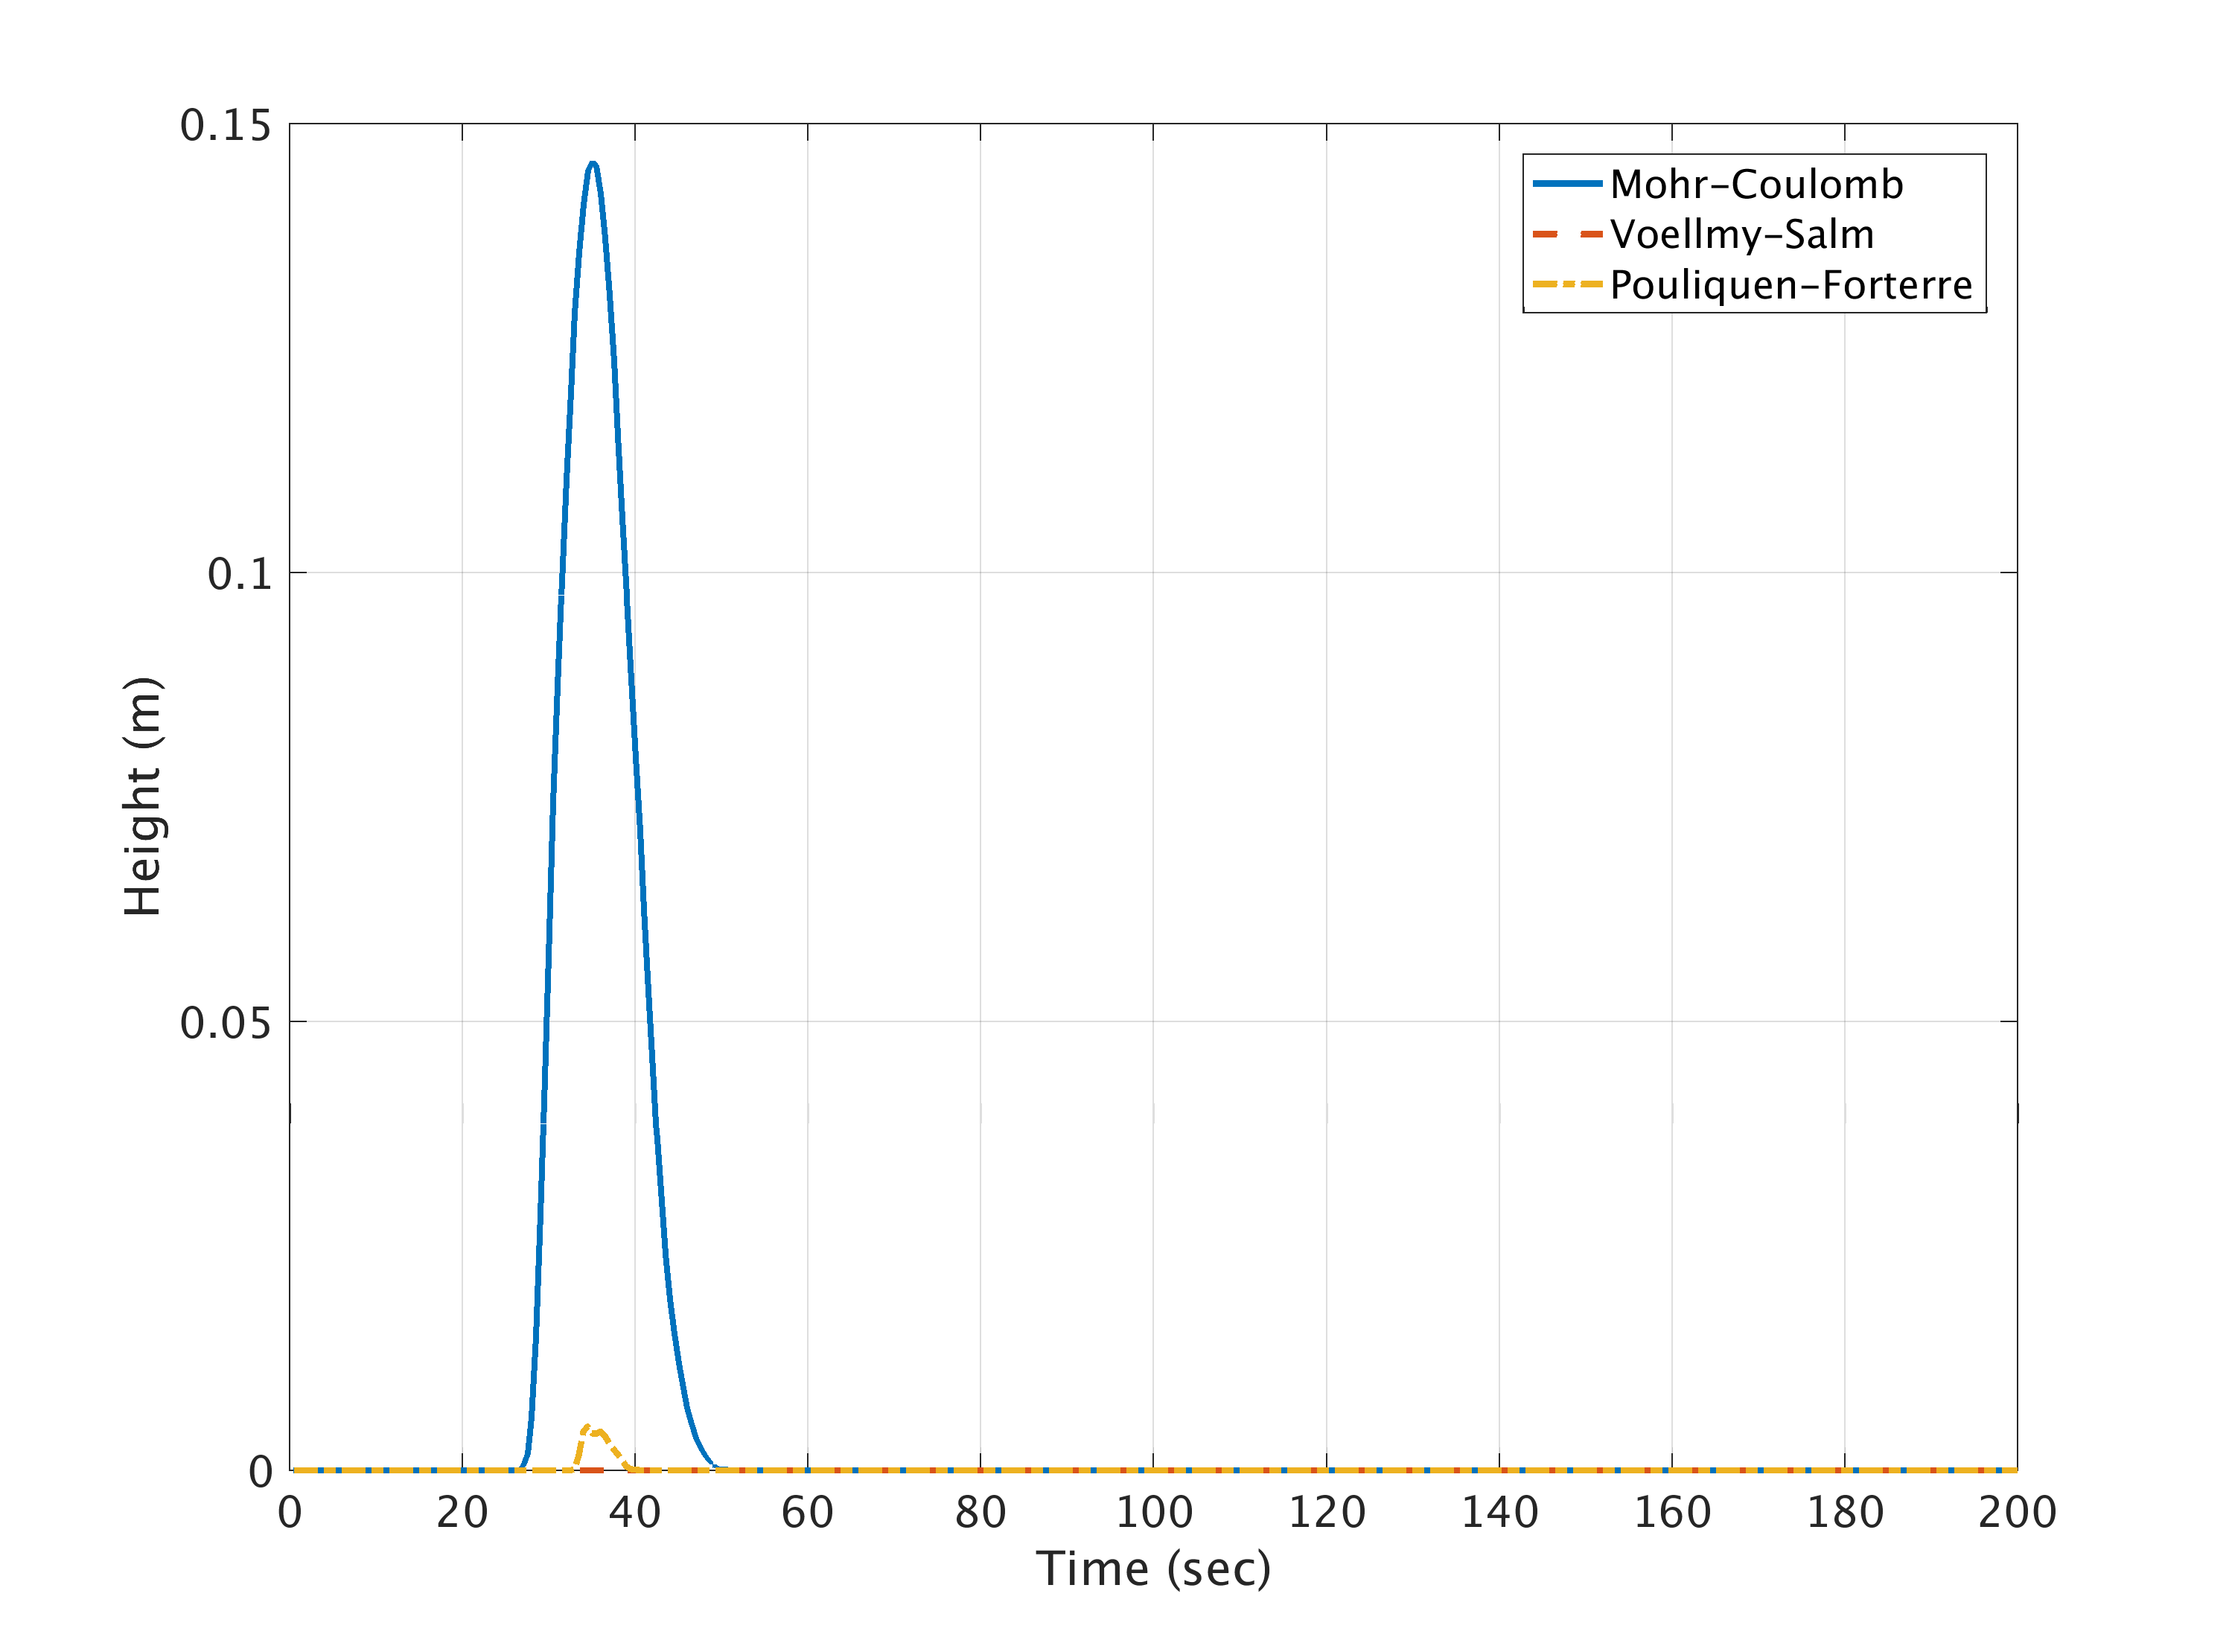
\includegraphics[width=1\textwidth]{HeightMeans/H7All.png}     
        \subcaption{Flow Height Records, Location 7.}
        \label{fig:MFHR_L7}
	\end{minipage}
	\begin{minipage}[b]{0.5\linewidth}
	\centering
    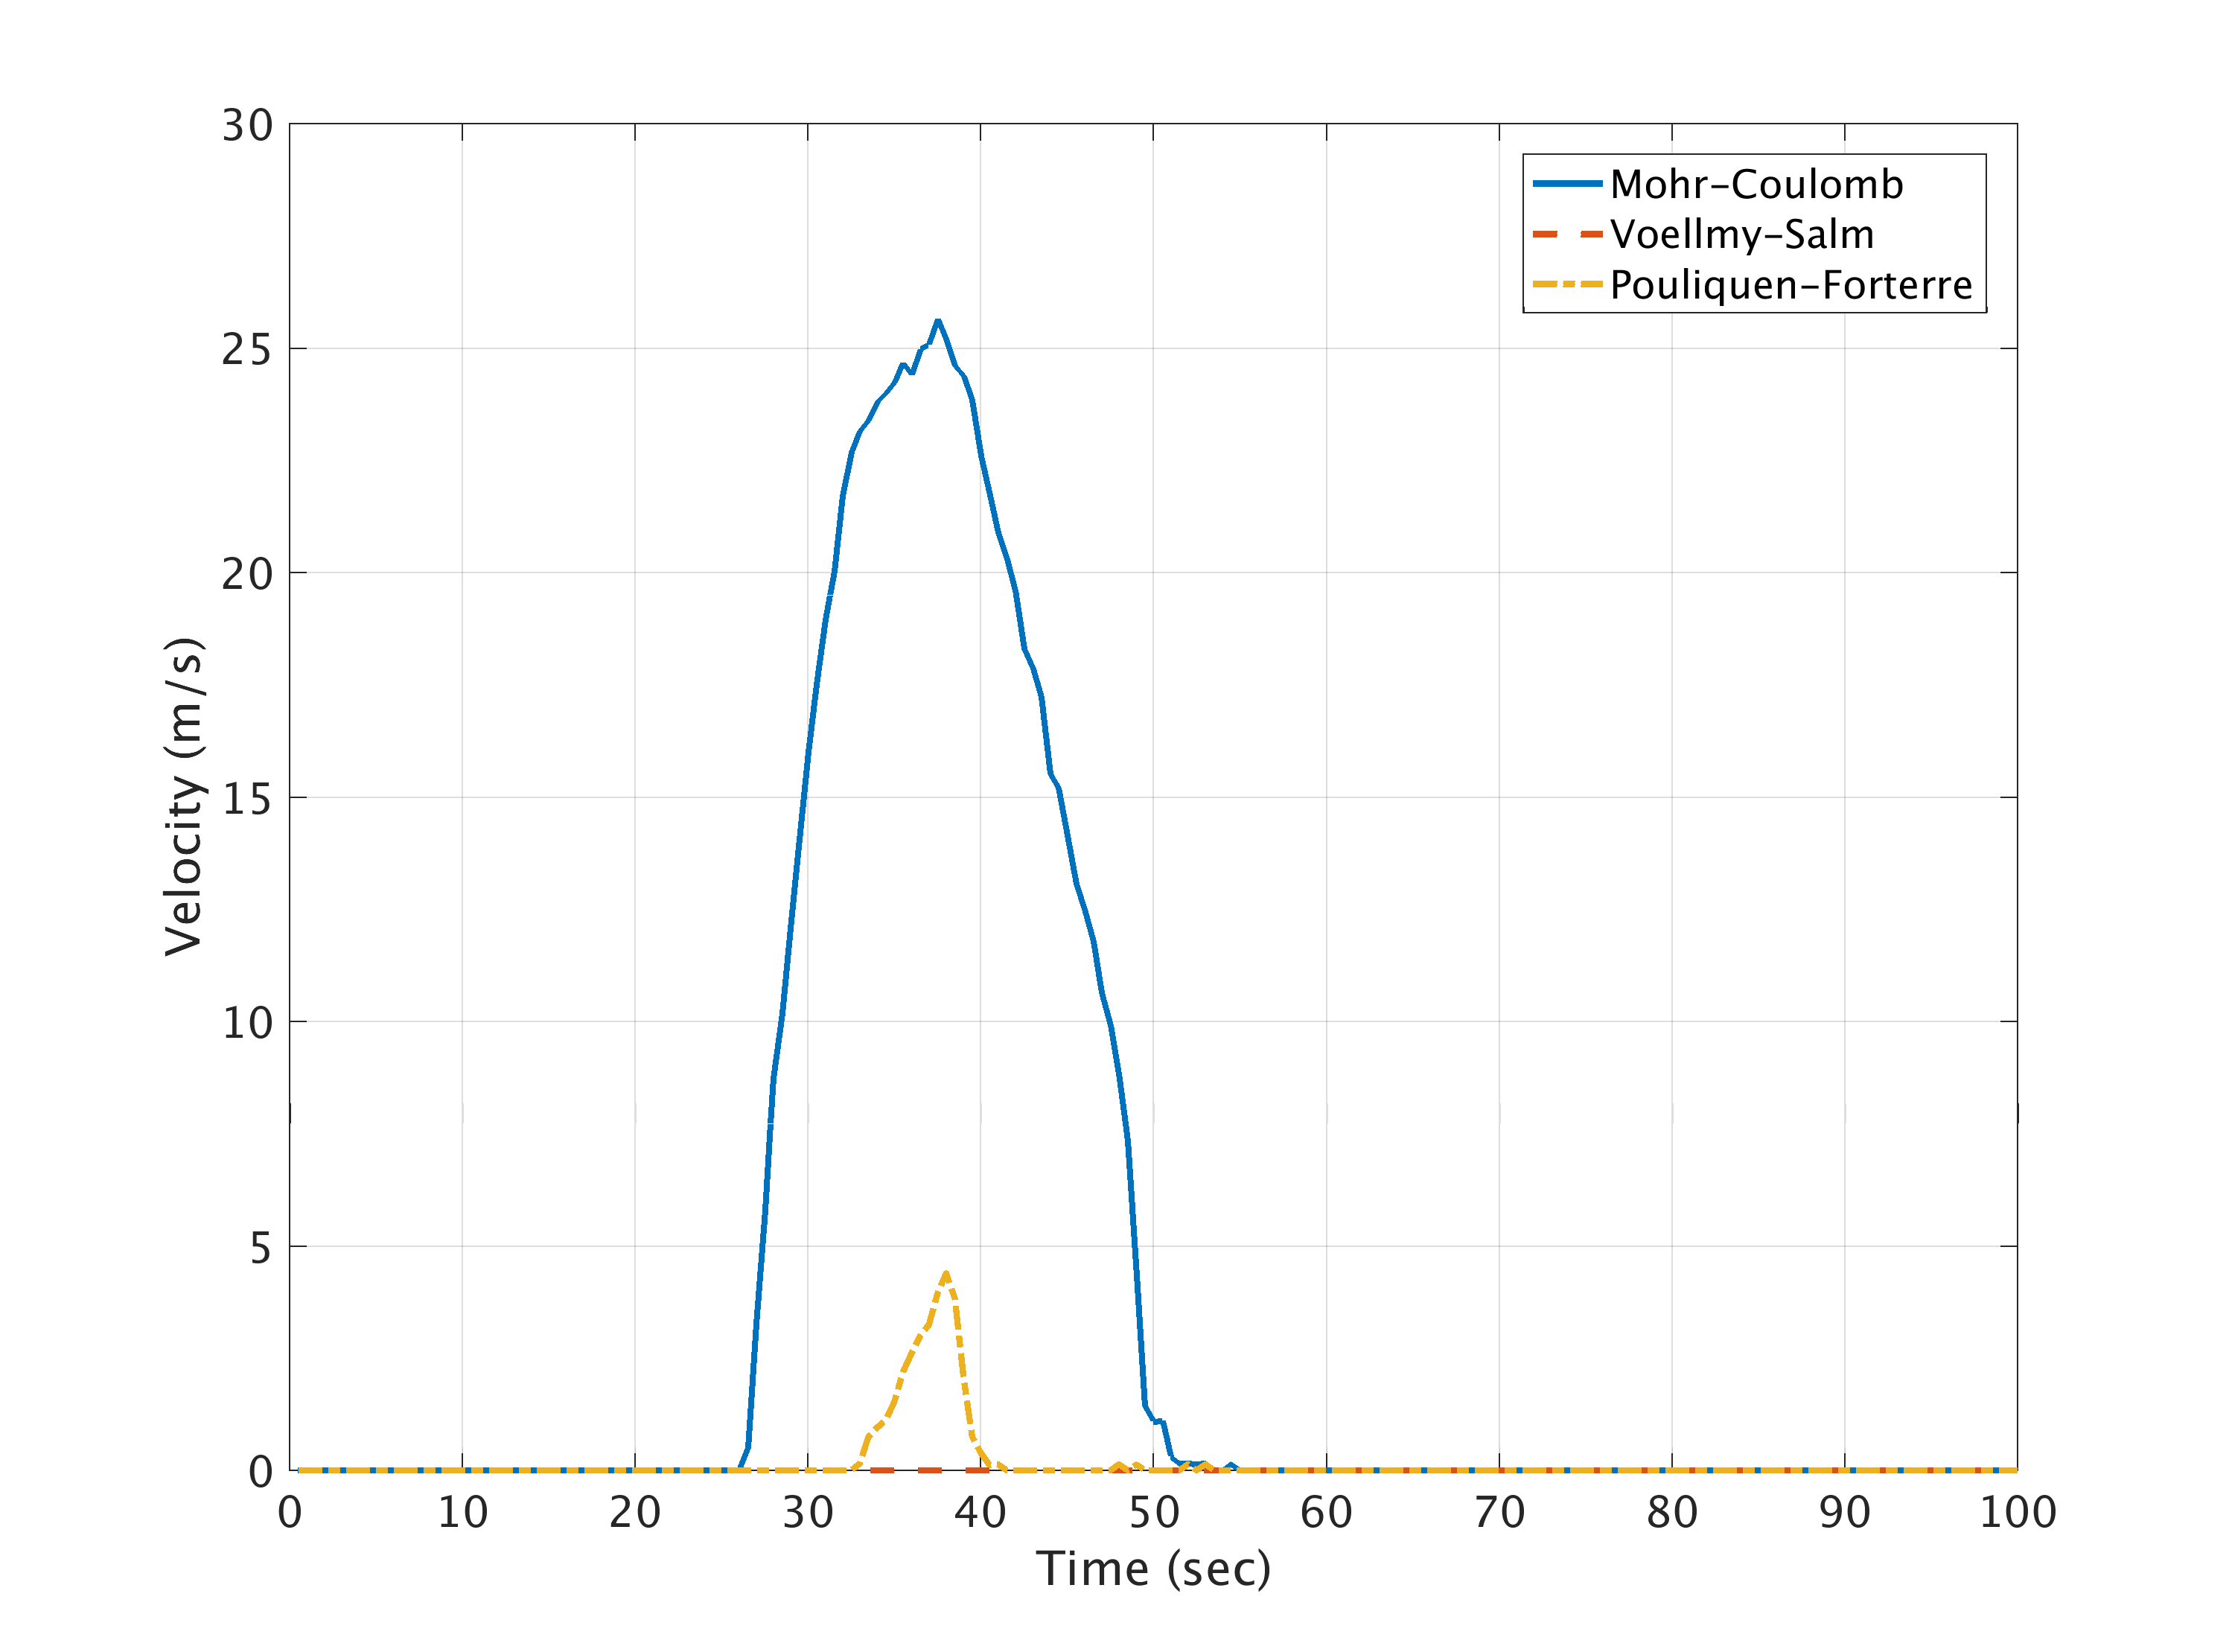
\includegraphics[width=1\textwidth]{VelocityMeans/V7All.png}
        \subcaption{Flow Velocity Records, Location 7.}
        \label{fig:MFVR_L7}
	\end{minipage}
	
	\begin{minipage}[b]{0.5\linewidth}
	\centering
    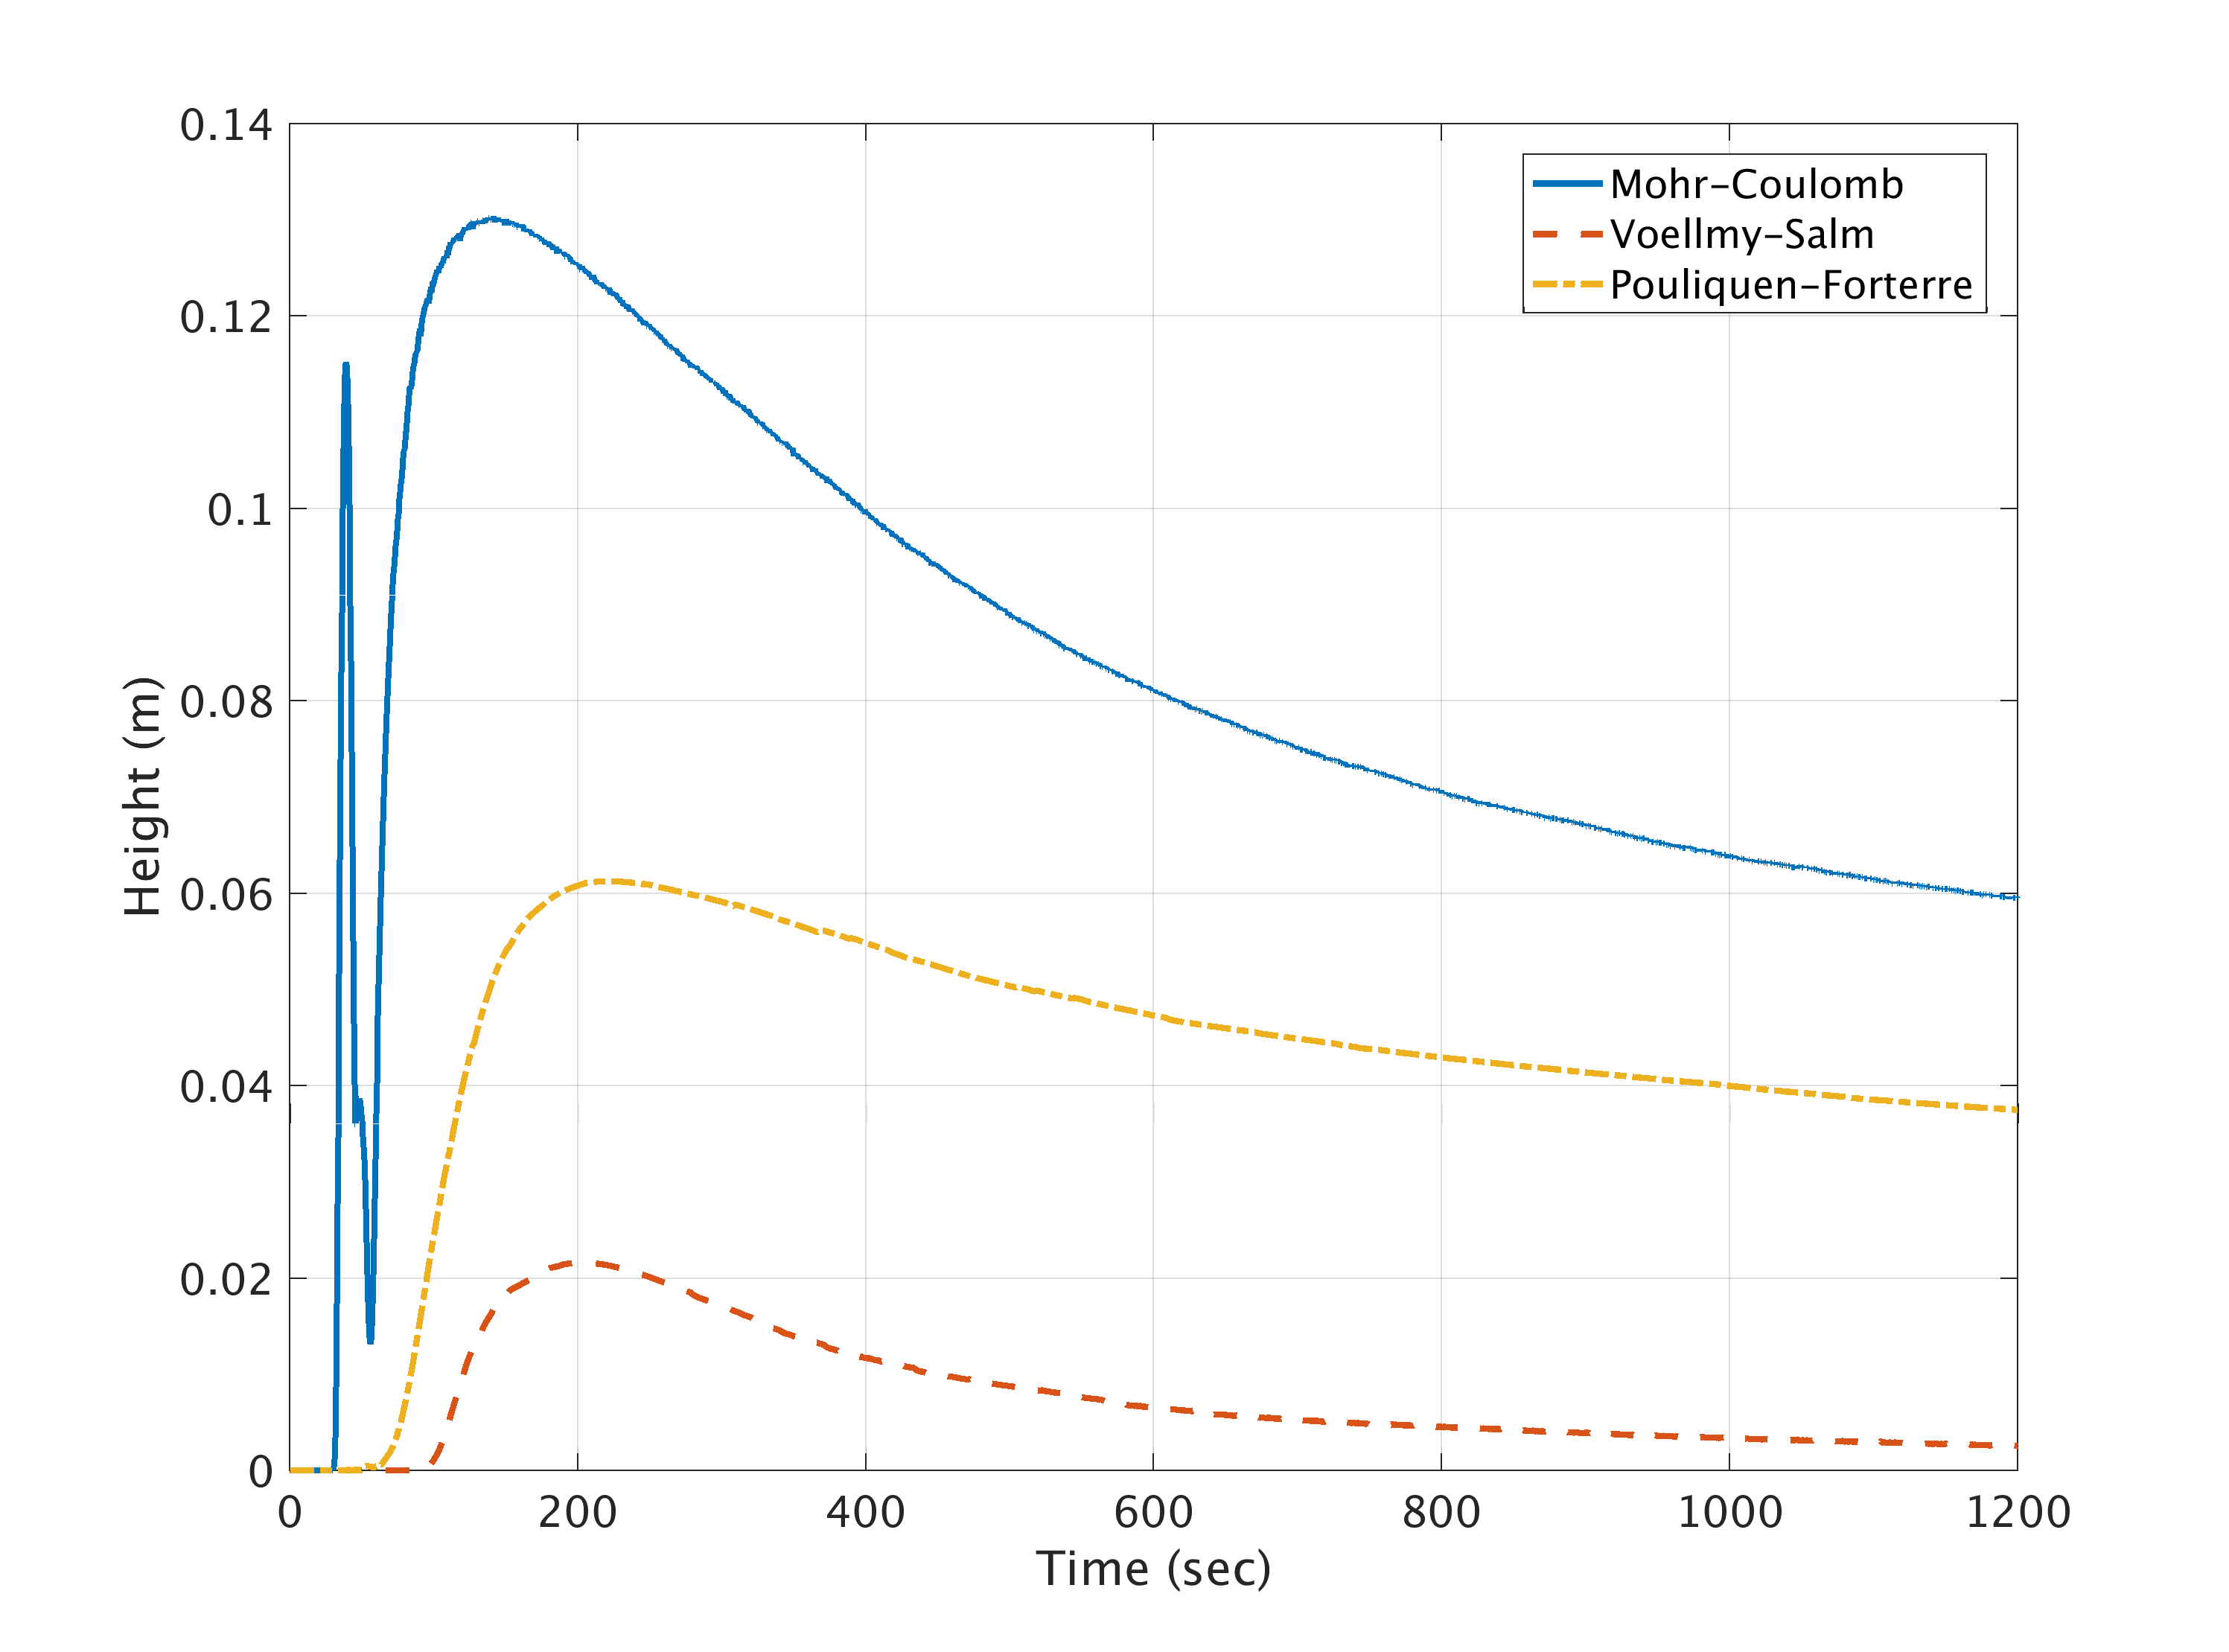
\includegraphics[width=1\textwidth]{HeightMeans/H8All.png}     
        \subcaption{Flow Height Records, Location 8.}
        \label{fig:MFHR_L8}
	\end{minipage}
	\begin{minipage}[b]{0.5\linewidth}
	\centering
    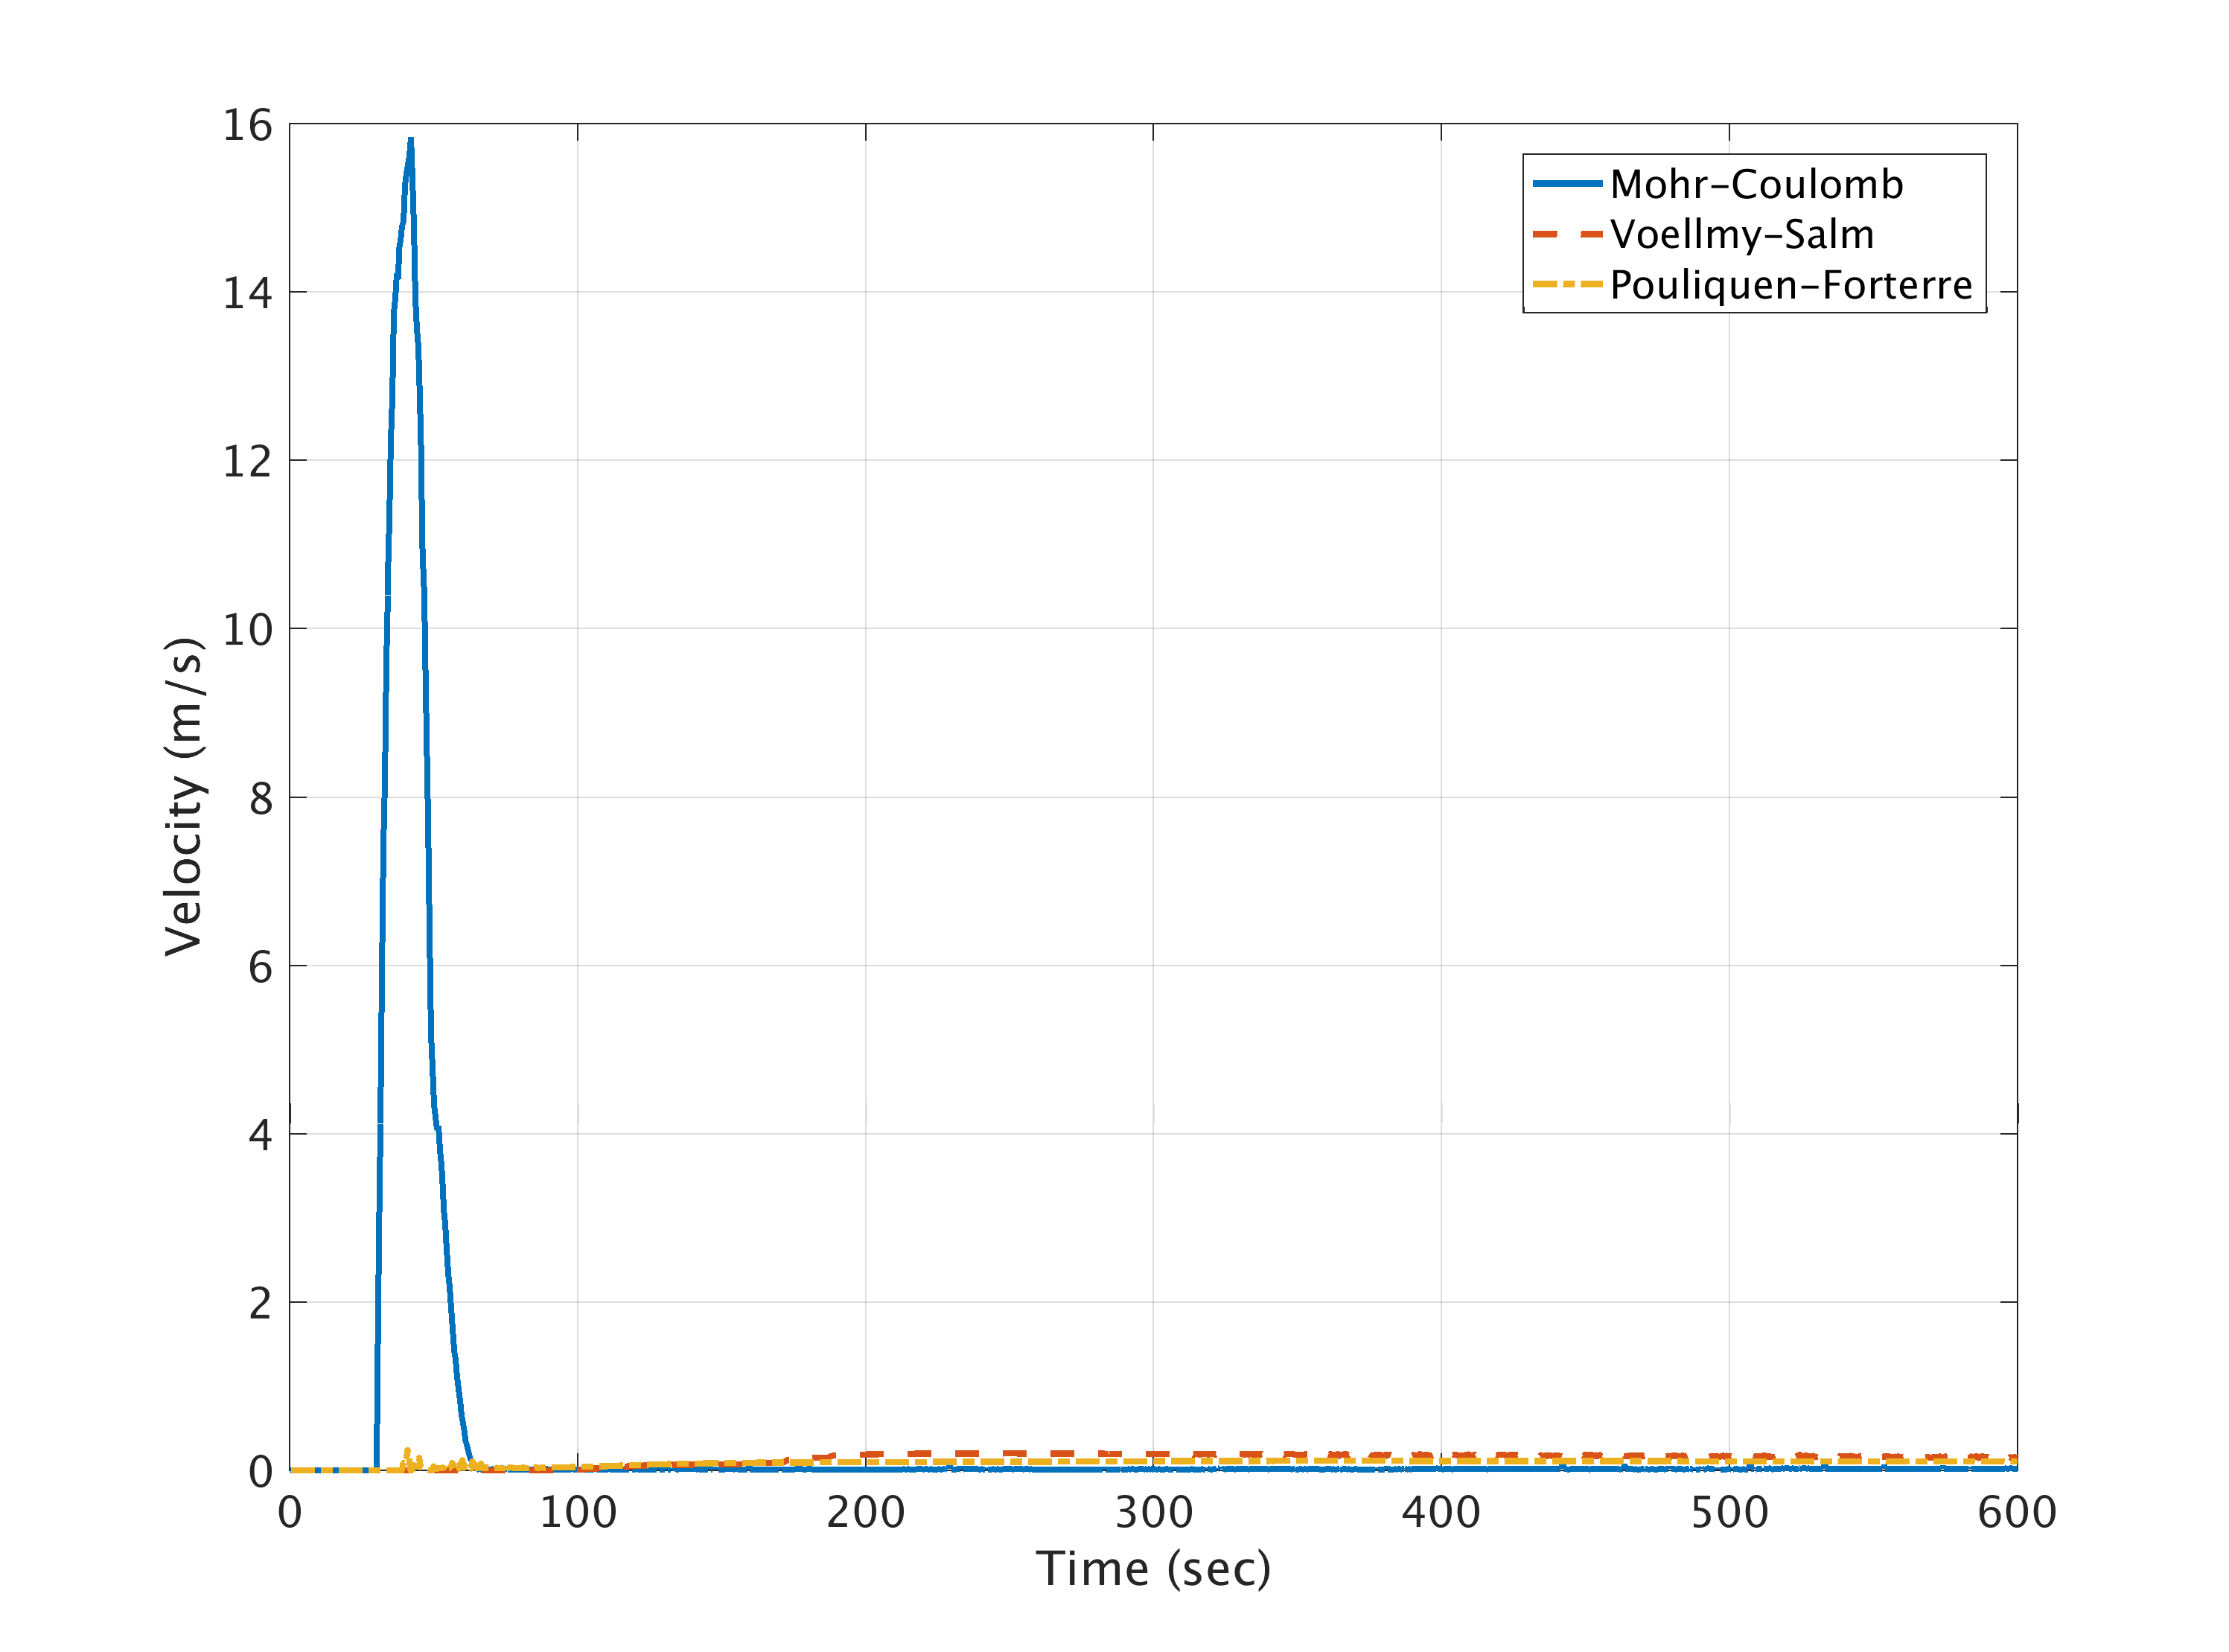
\includegraphics[width=1\textwidth]{VelocityMeans/V8All.png}
        \subcaption{Flow Velocity Records, Location 8.}
        \label{fig:MFVR_L8}
	\end{minipage}
	
	\begin{minipage}[b]{0.5\linewidth}
	\centering
    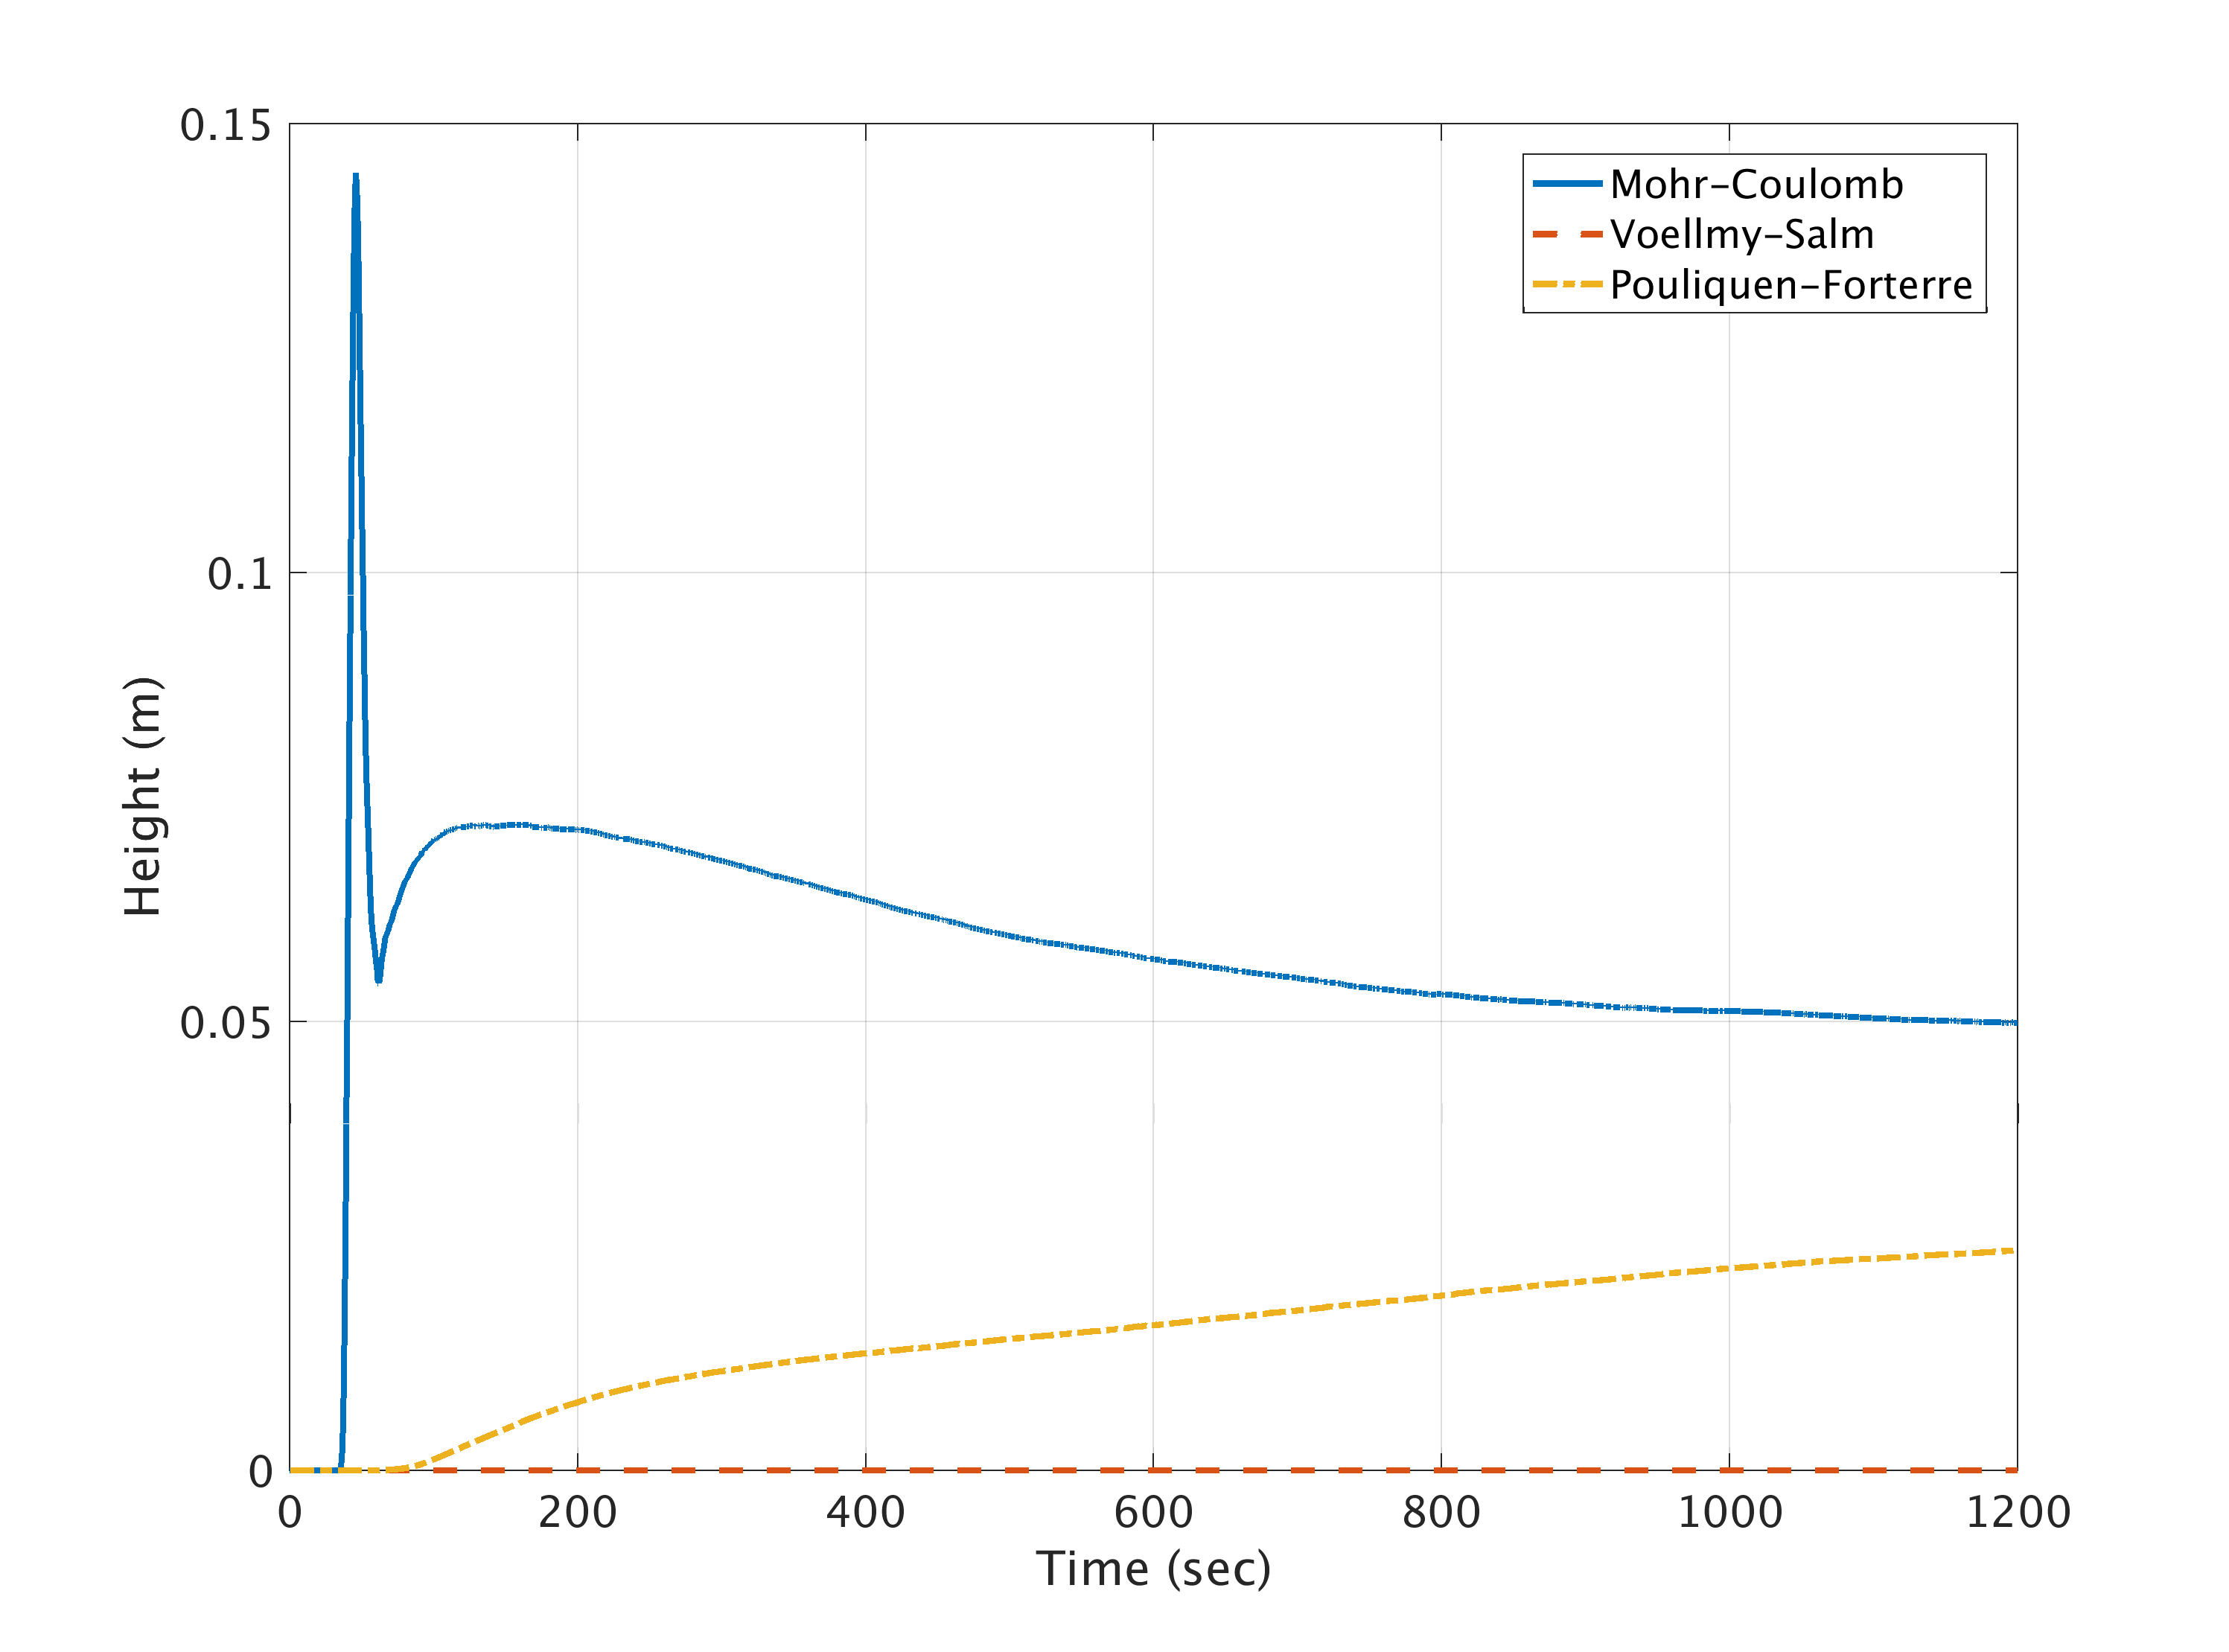
\includegraphics[width=1\textwidth]{HeightMeans/H9All.png}     
        \subcaption{Flow Height Records, Location 9.}
        \label{fig:MFHR_L9}
	\end{minipage}
	\begin{minipage}[b]{0.5\linewidth}
	\centering
    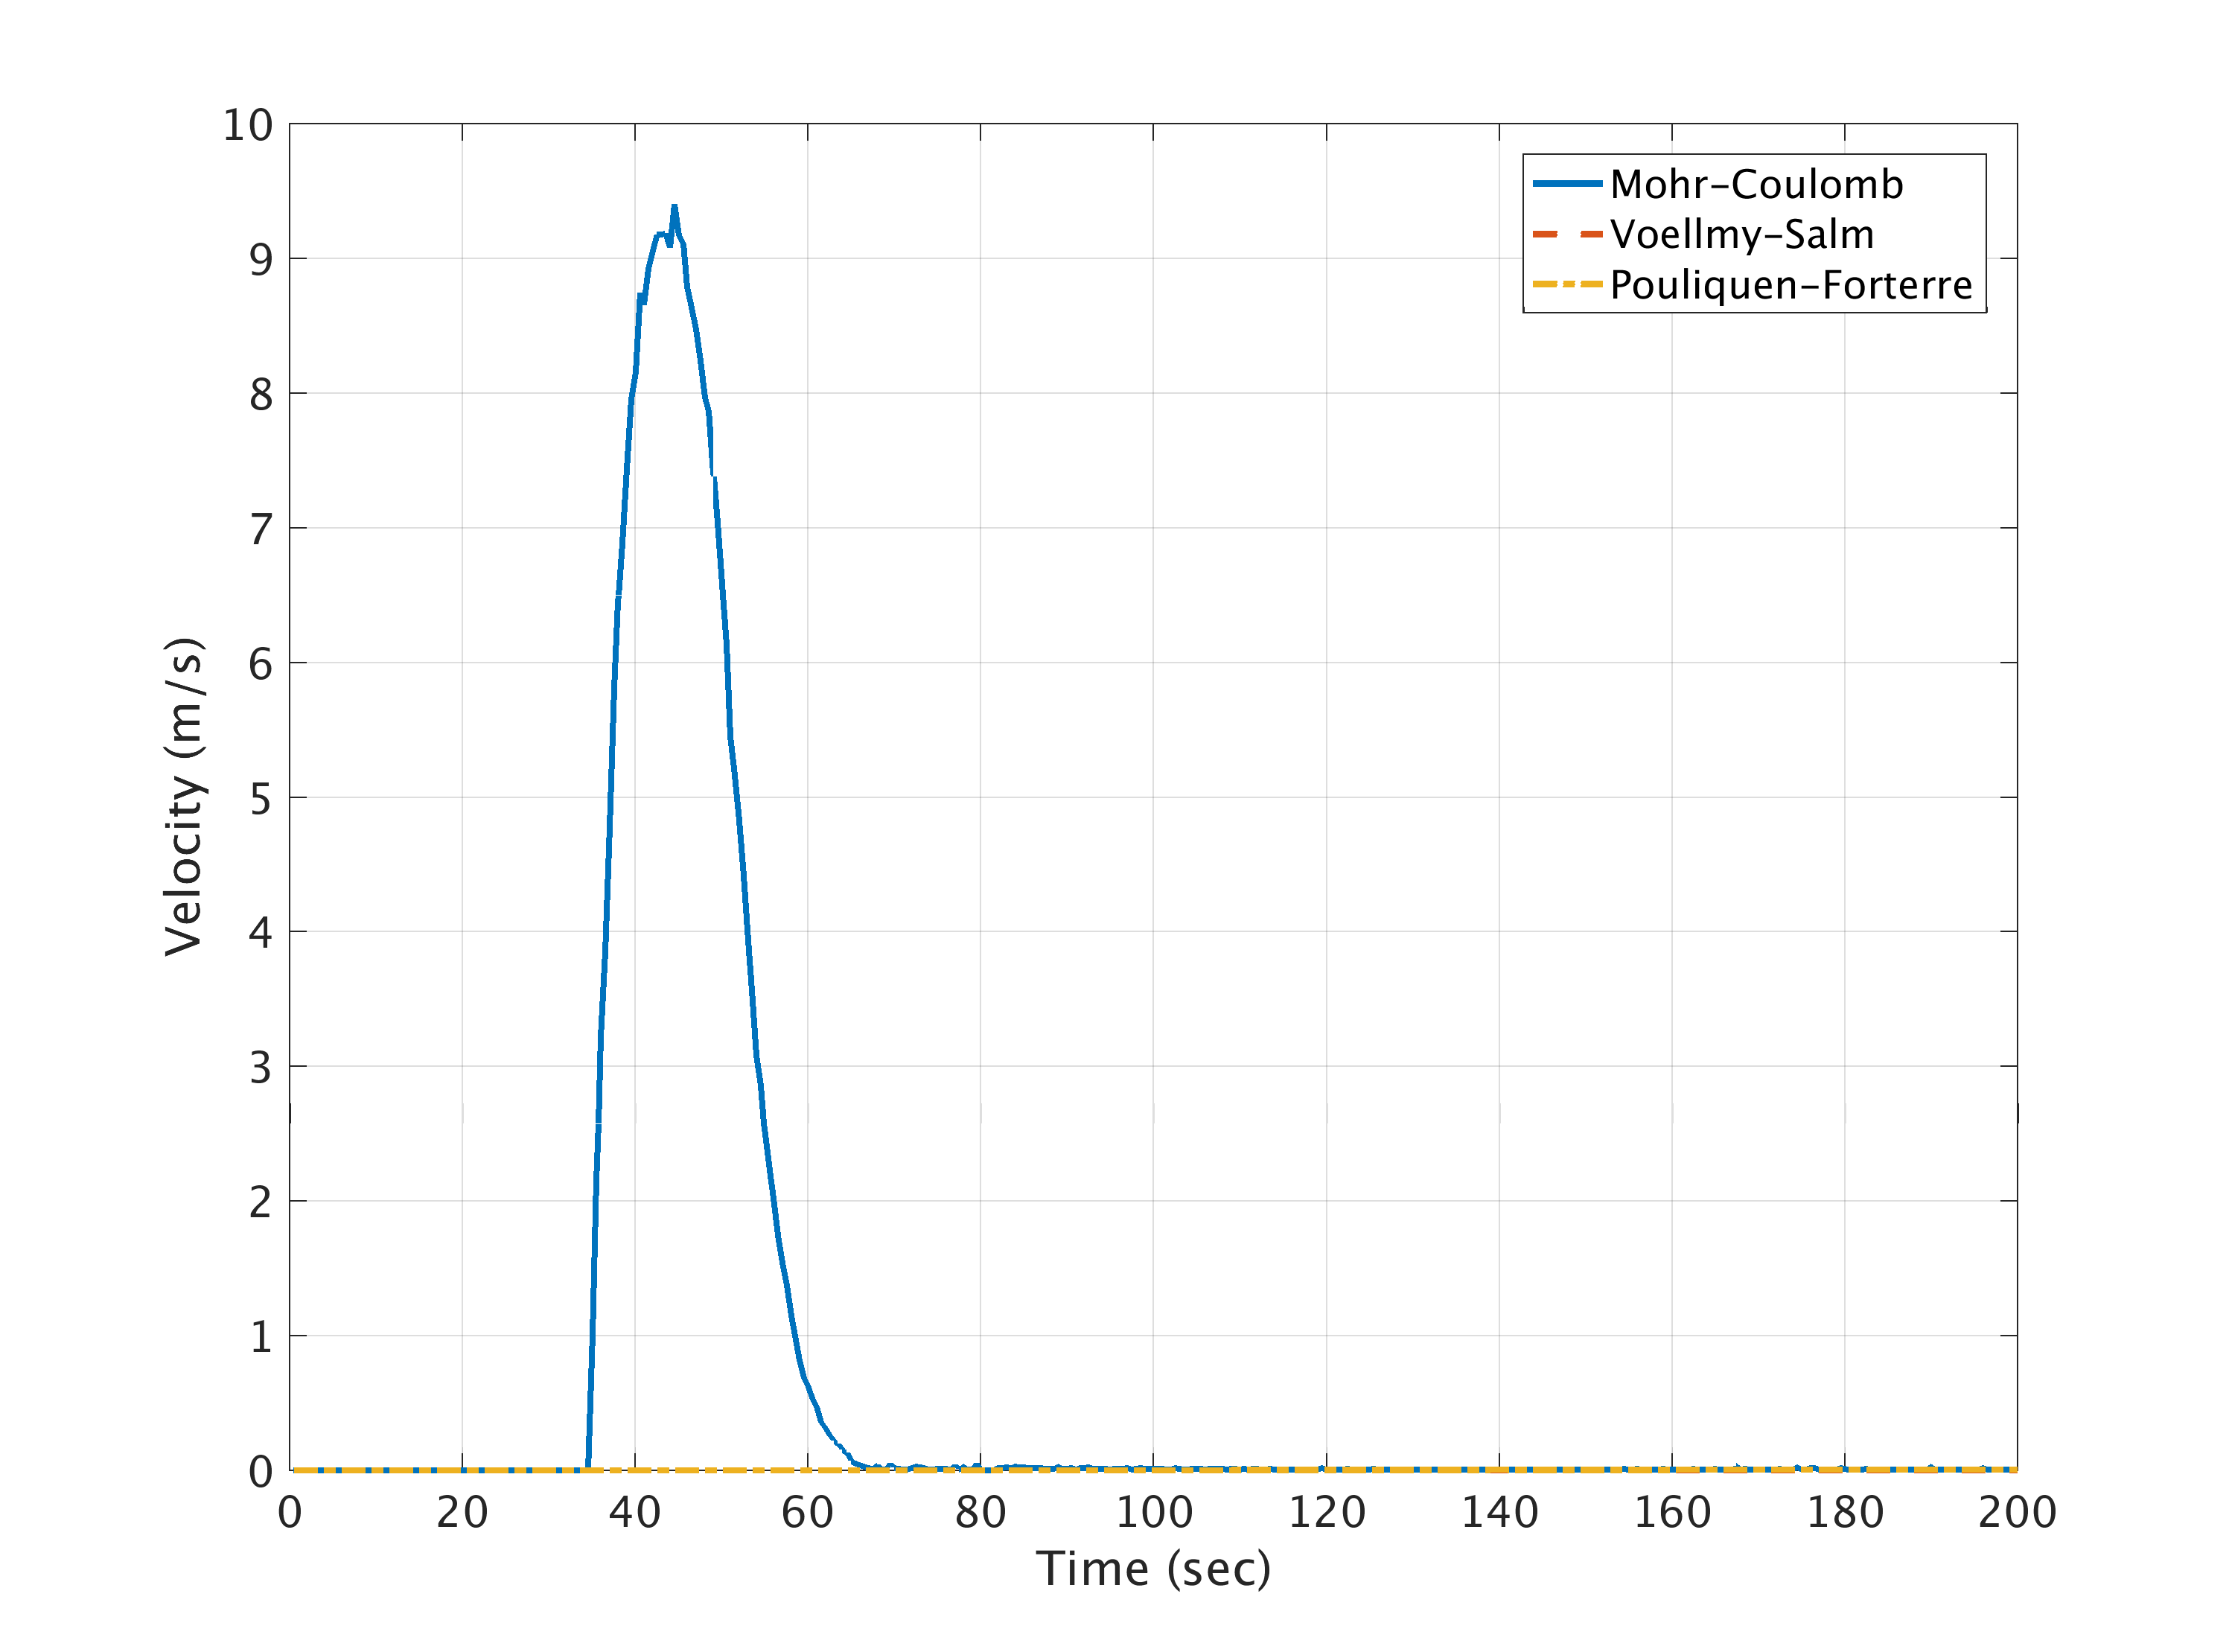
\includegraphics[width=1\textwidth]{VelocityMeans/V9All.png}
        \subcaption{Flow Velocity Records, Location 9.}
        \label{fig:MFVR_L9}
	\end{minipage}
		
	\caption{Mean Values of Flow Height and Velocity Records at locations 7,8 and 9.}\label{fig:MFHVR_L789}	
\end{figure}

\begin{figure}[H]
	\begin{minipage}[b]{0.5\linewidth}
	\centering
    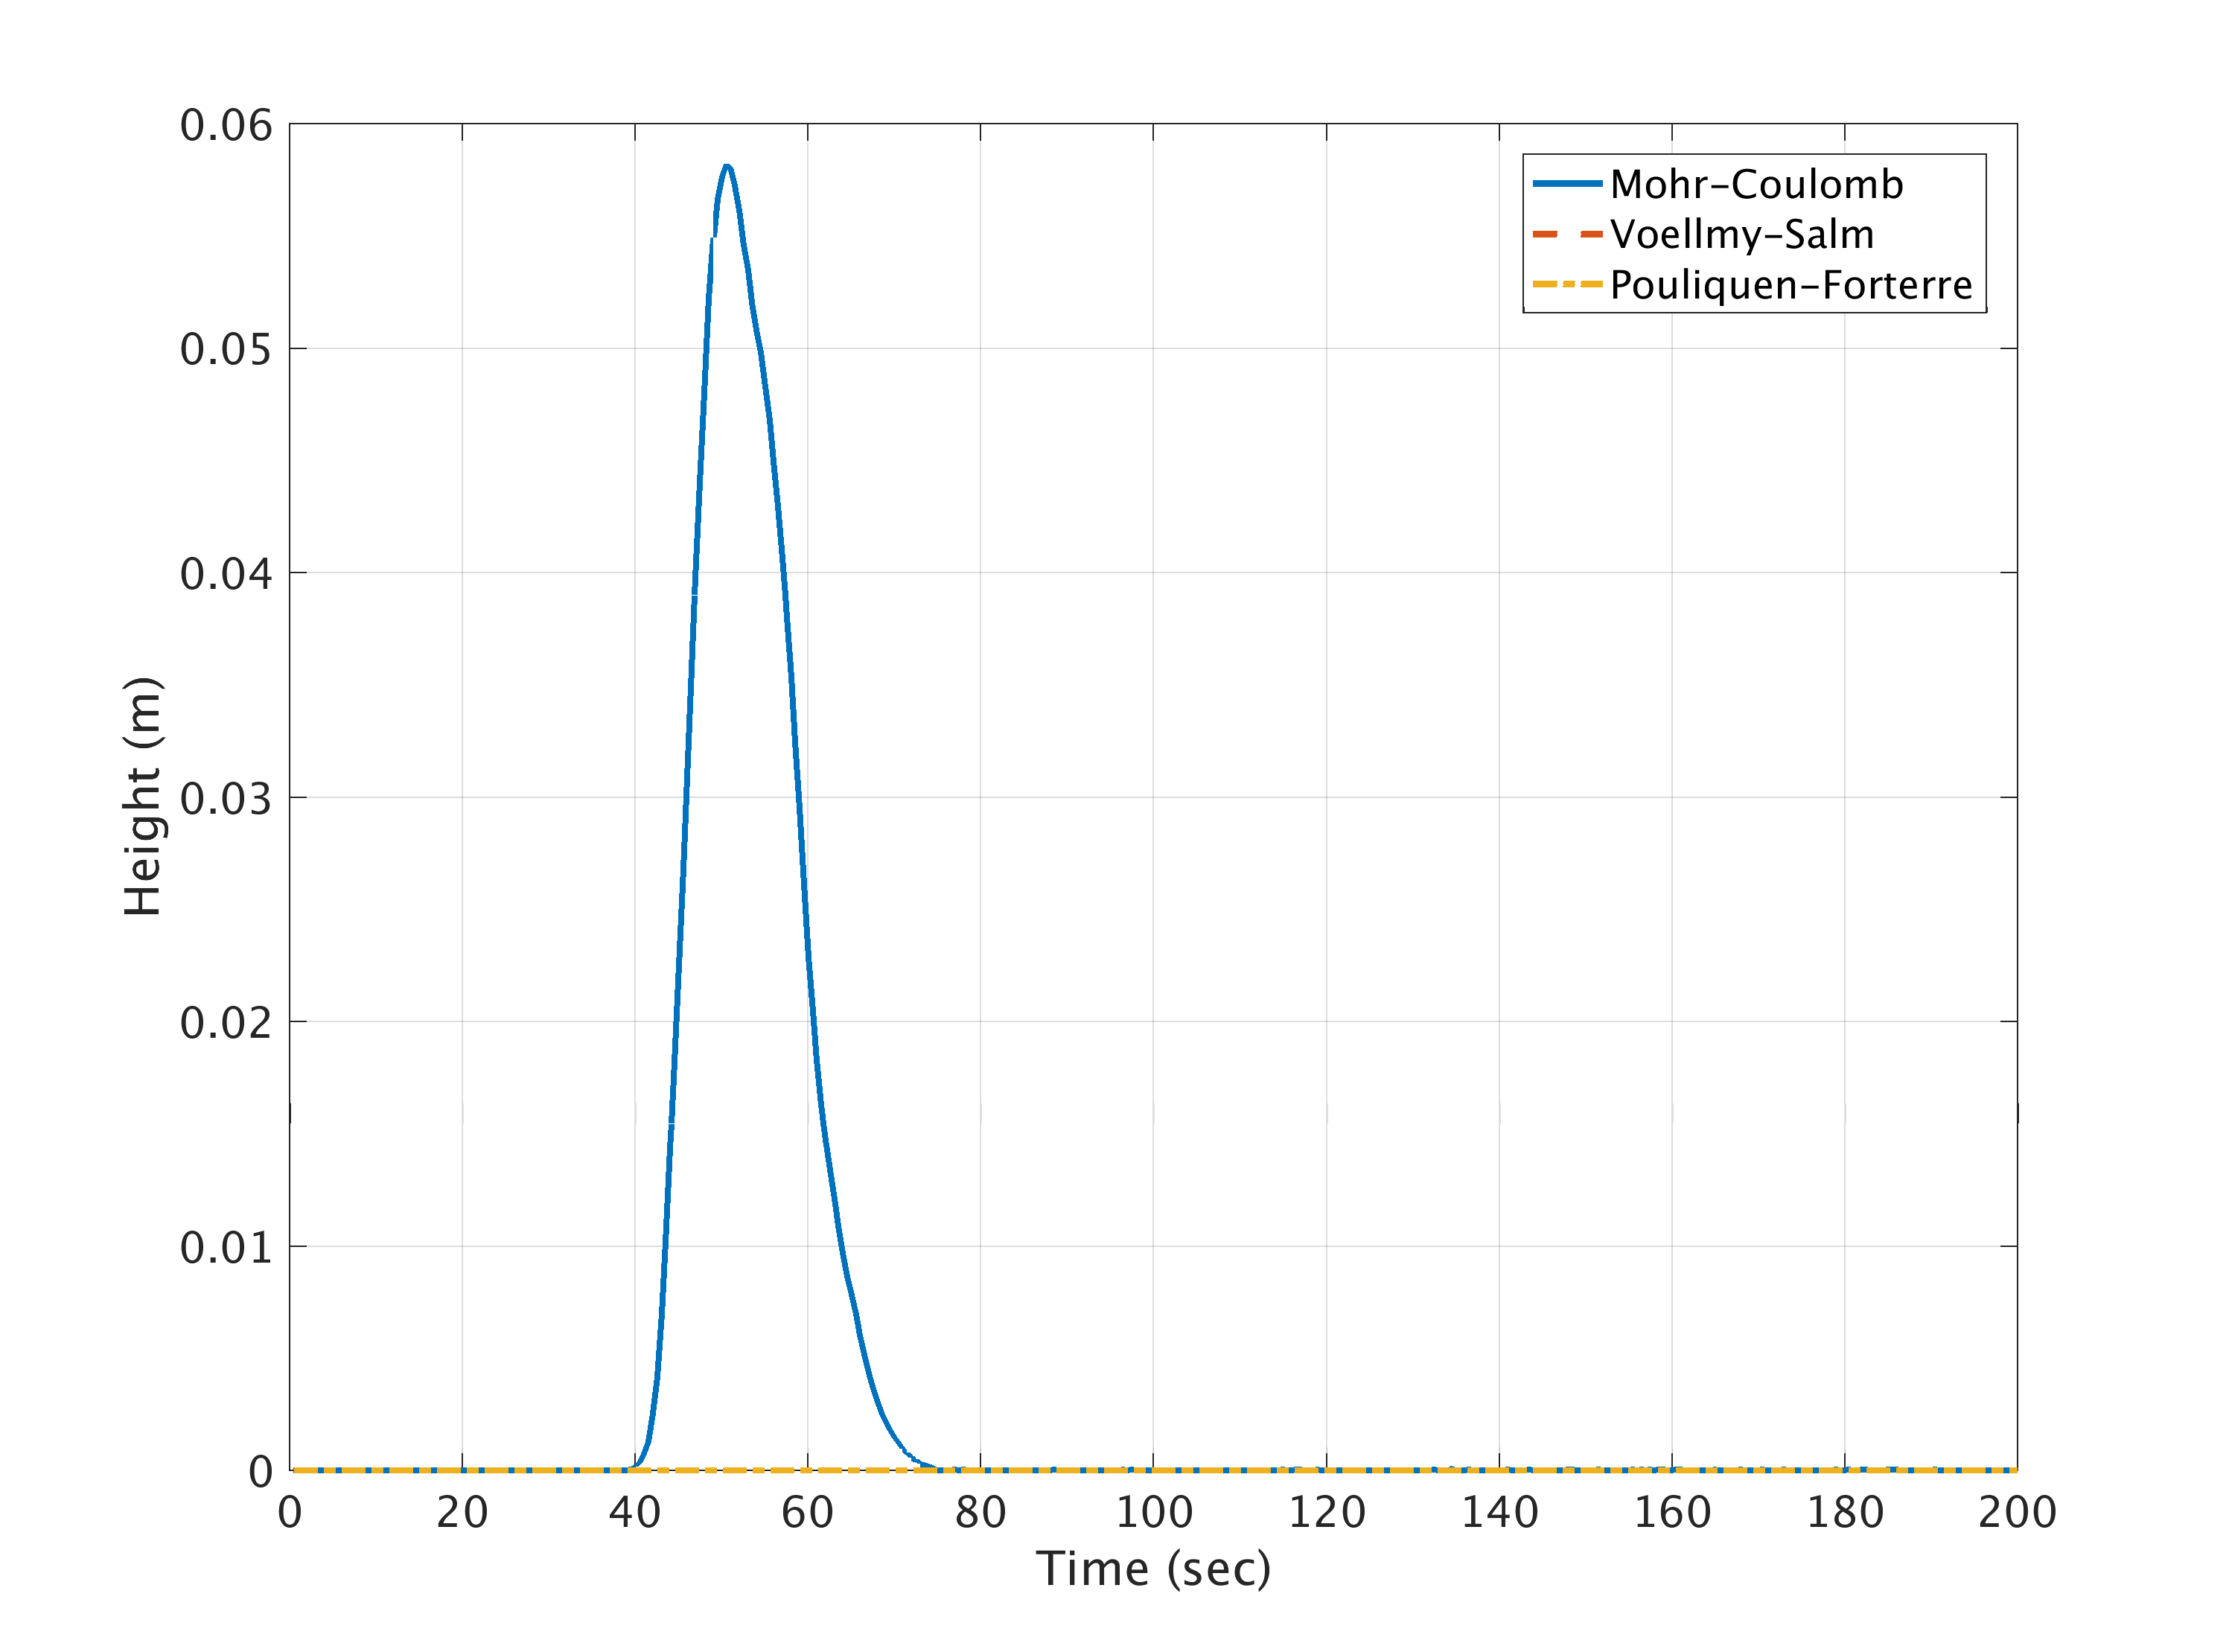
\includegraphics[width=1\textwidth]{HeightMeans/H10All.png}     
        \subcaption{Flow Height Records, Location 10.}
        \label{fig:MFHR_L10}
	\end{minipage}
	\begin{minipage}[b]{0.5\linewidth}
	\centering
    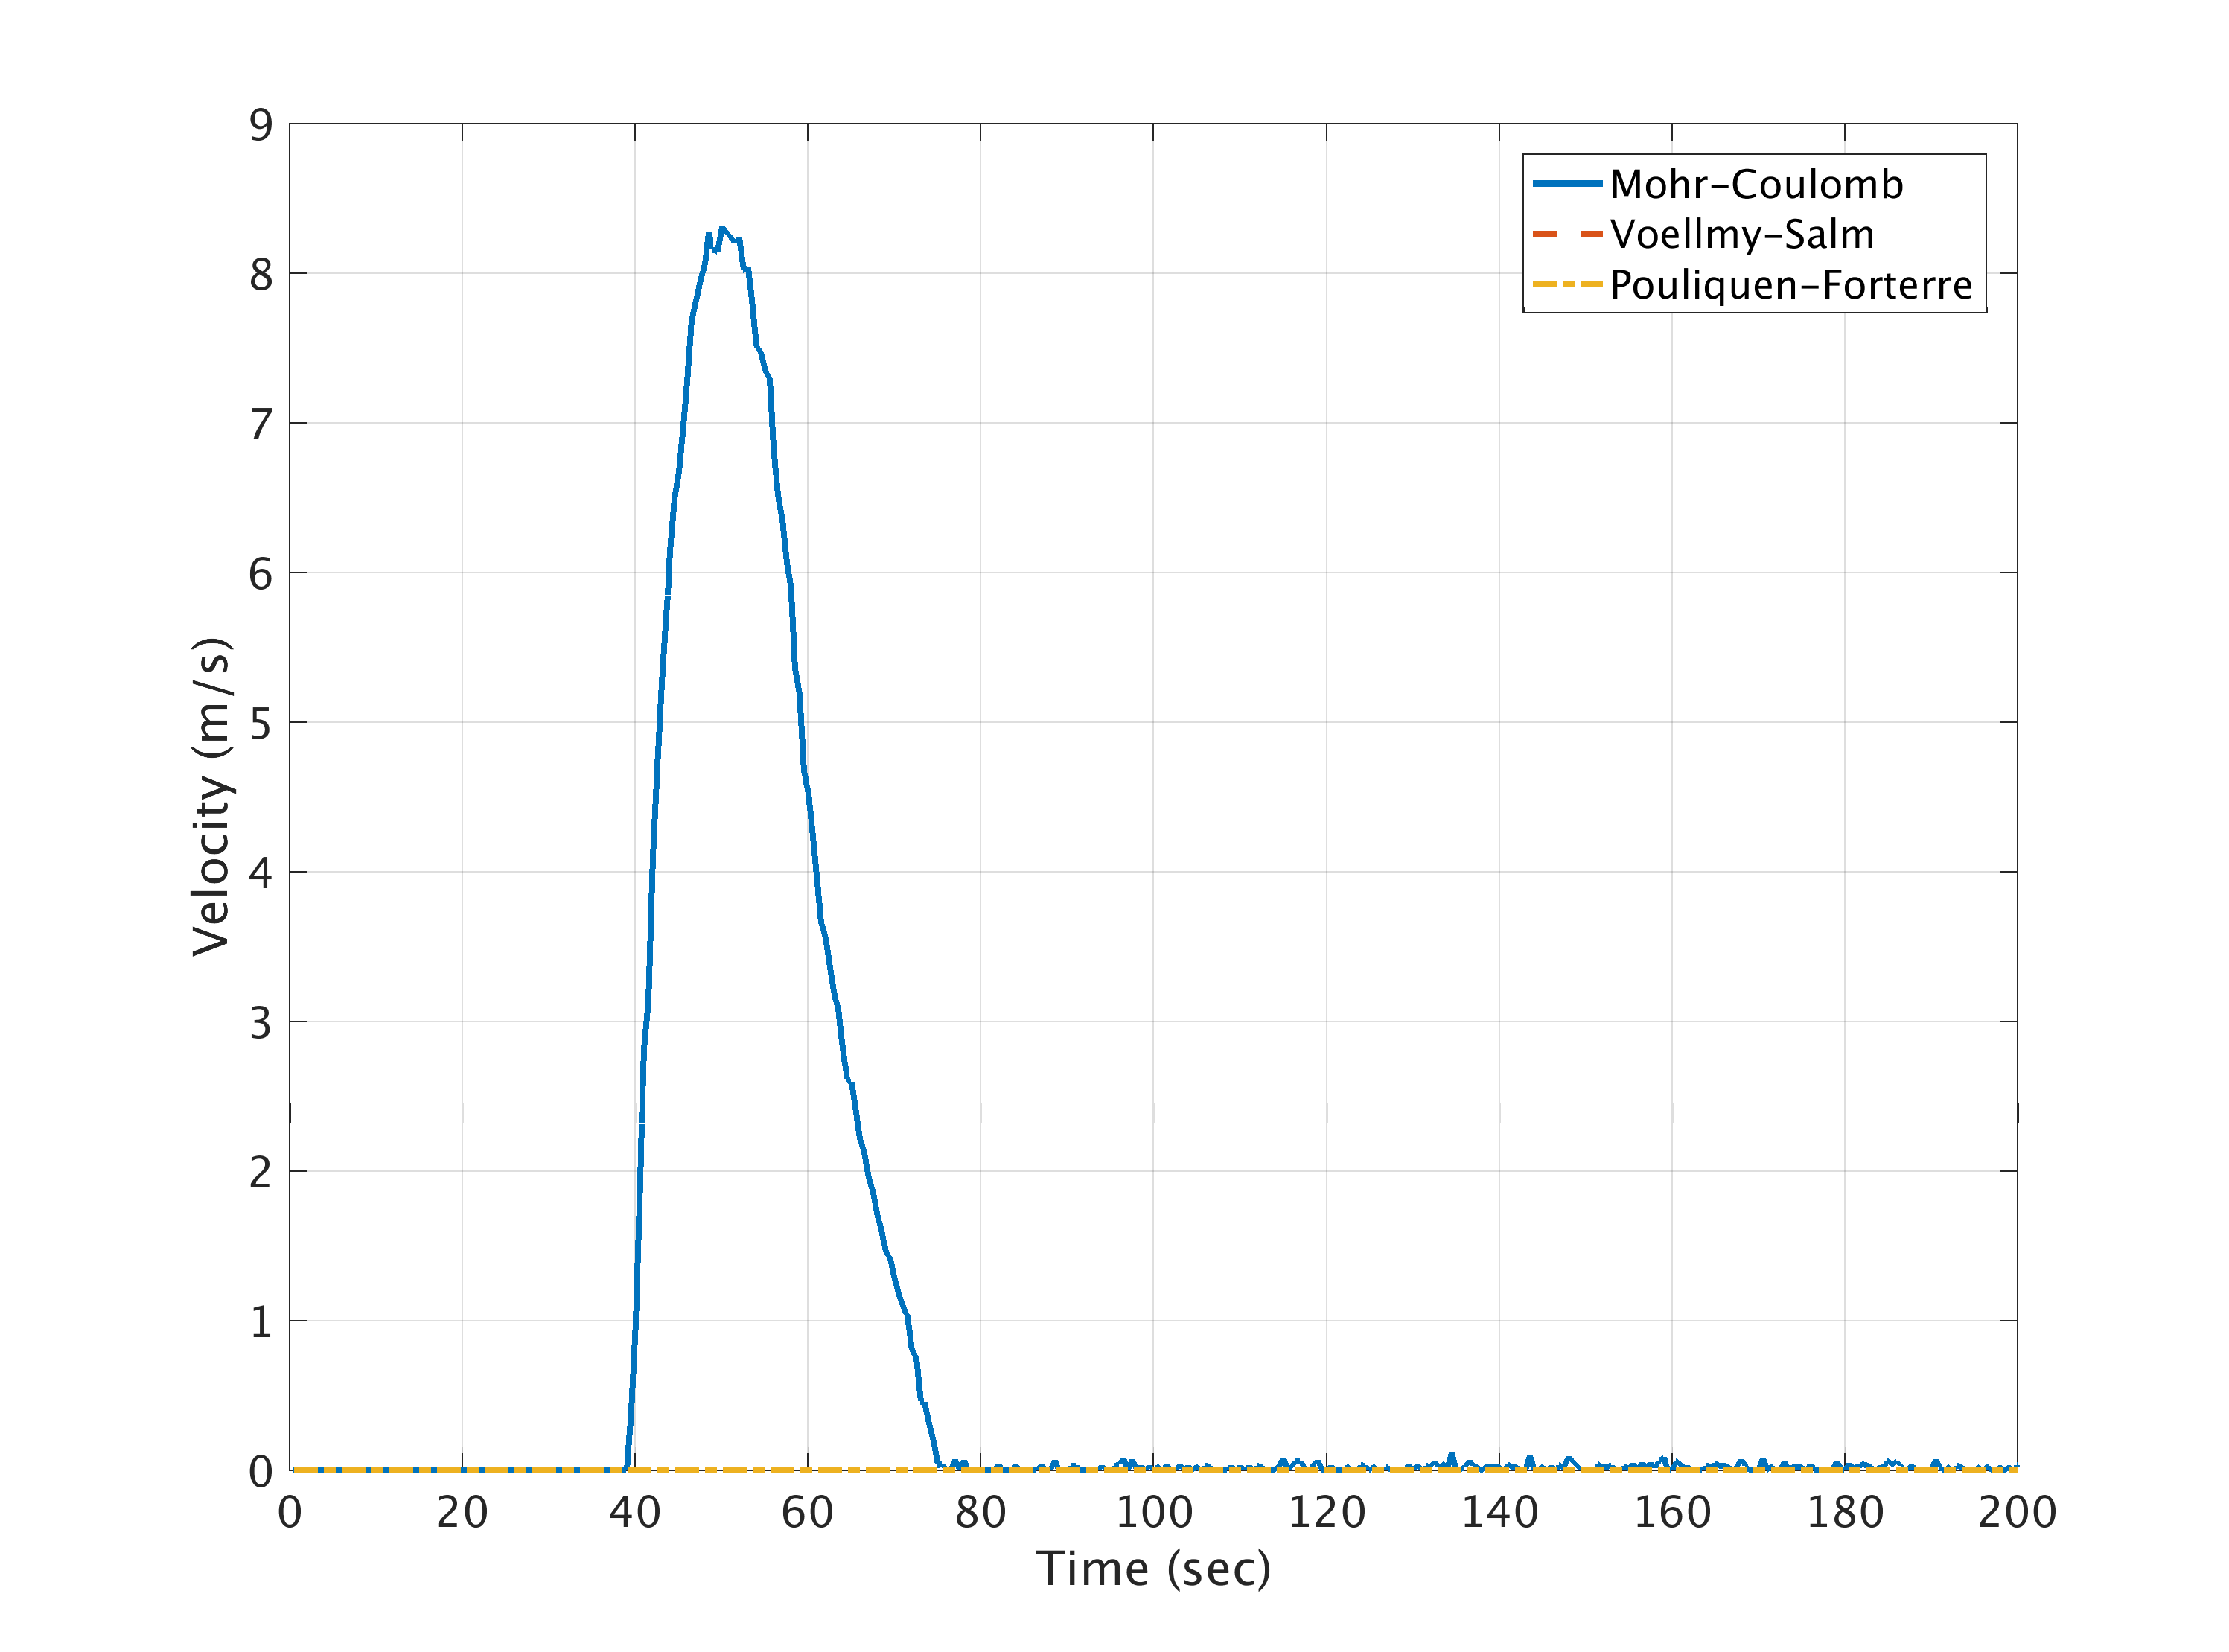
\includegraphics[width=1\textwidth]{VelocityMeans/V10All.png}
        \subcaption{Flow Velocity Records, Location 10.}
        \label{fig:MFVR_L10}
	\end{minipage}
	
	\begin{minipage}[b]{0.5\linewidth}
	\centering
    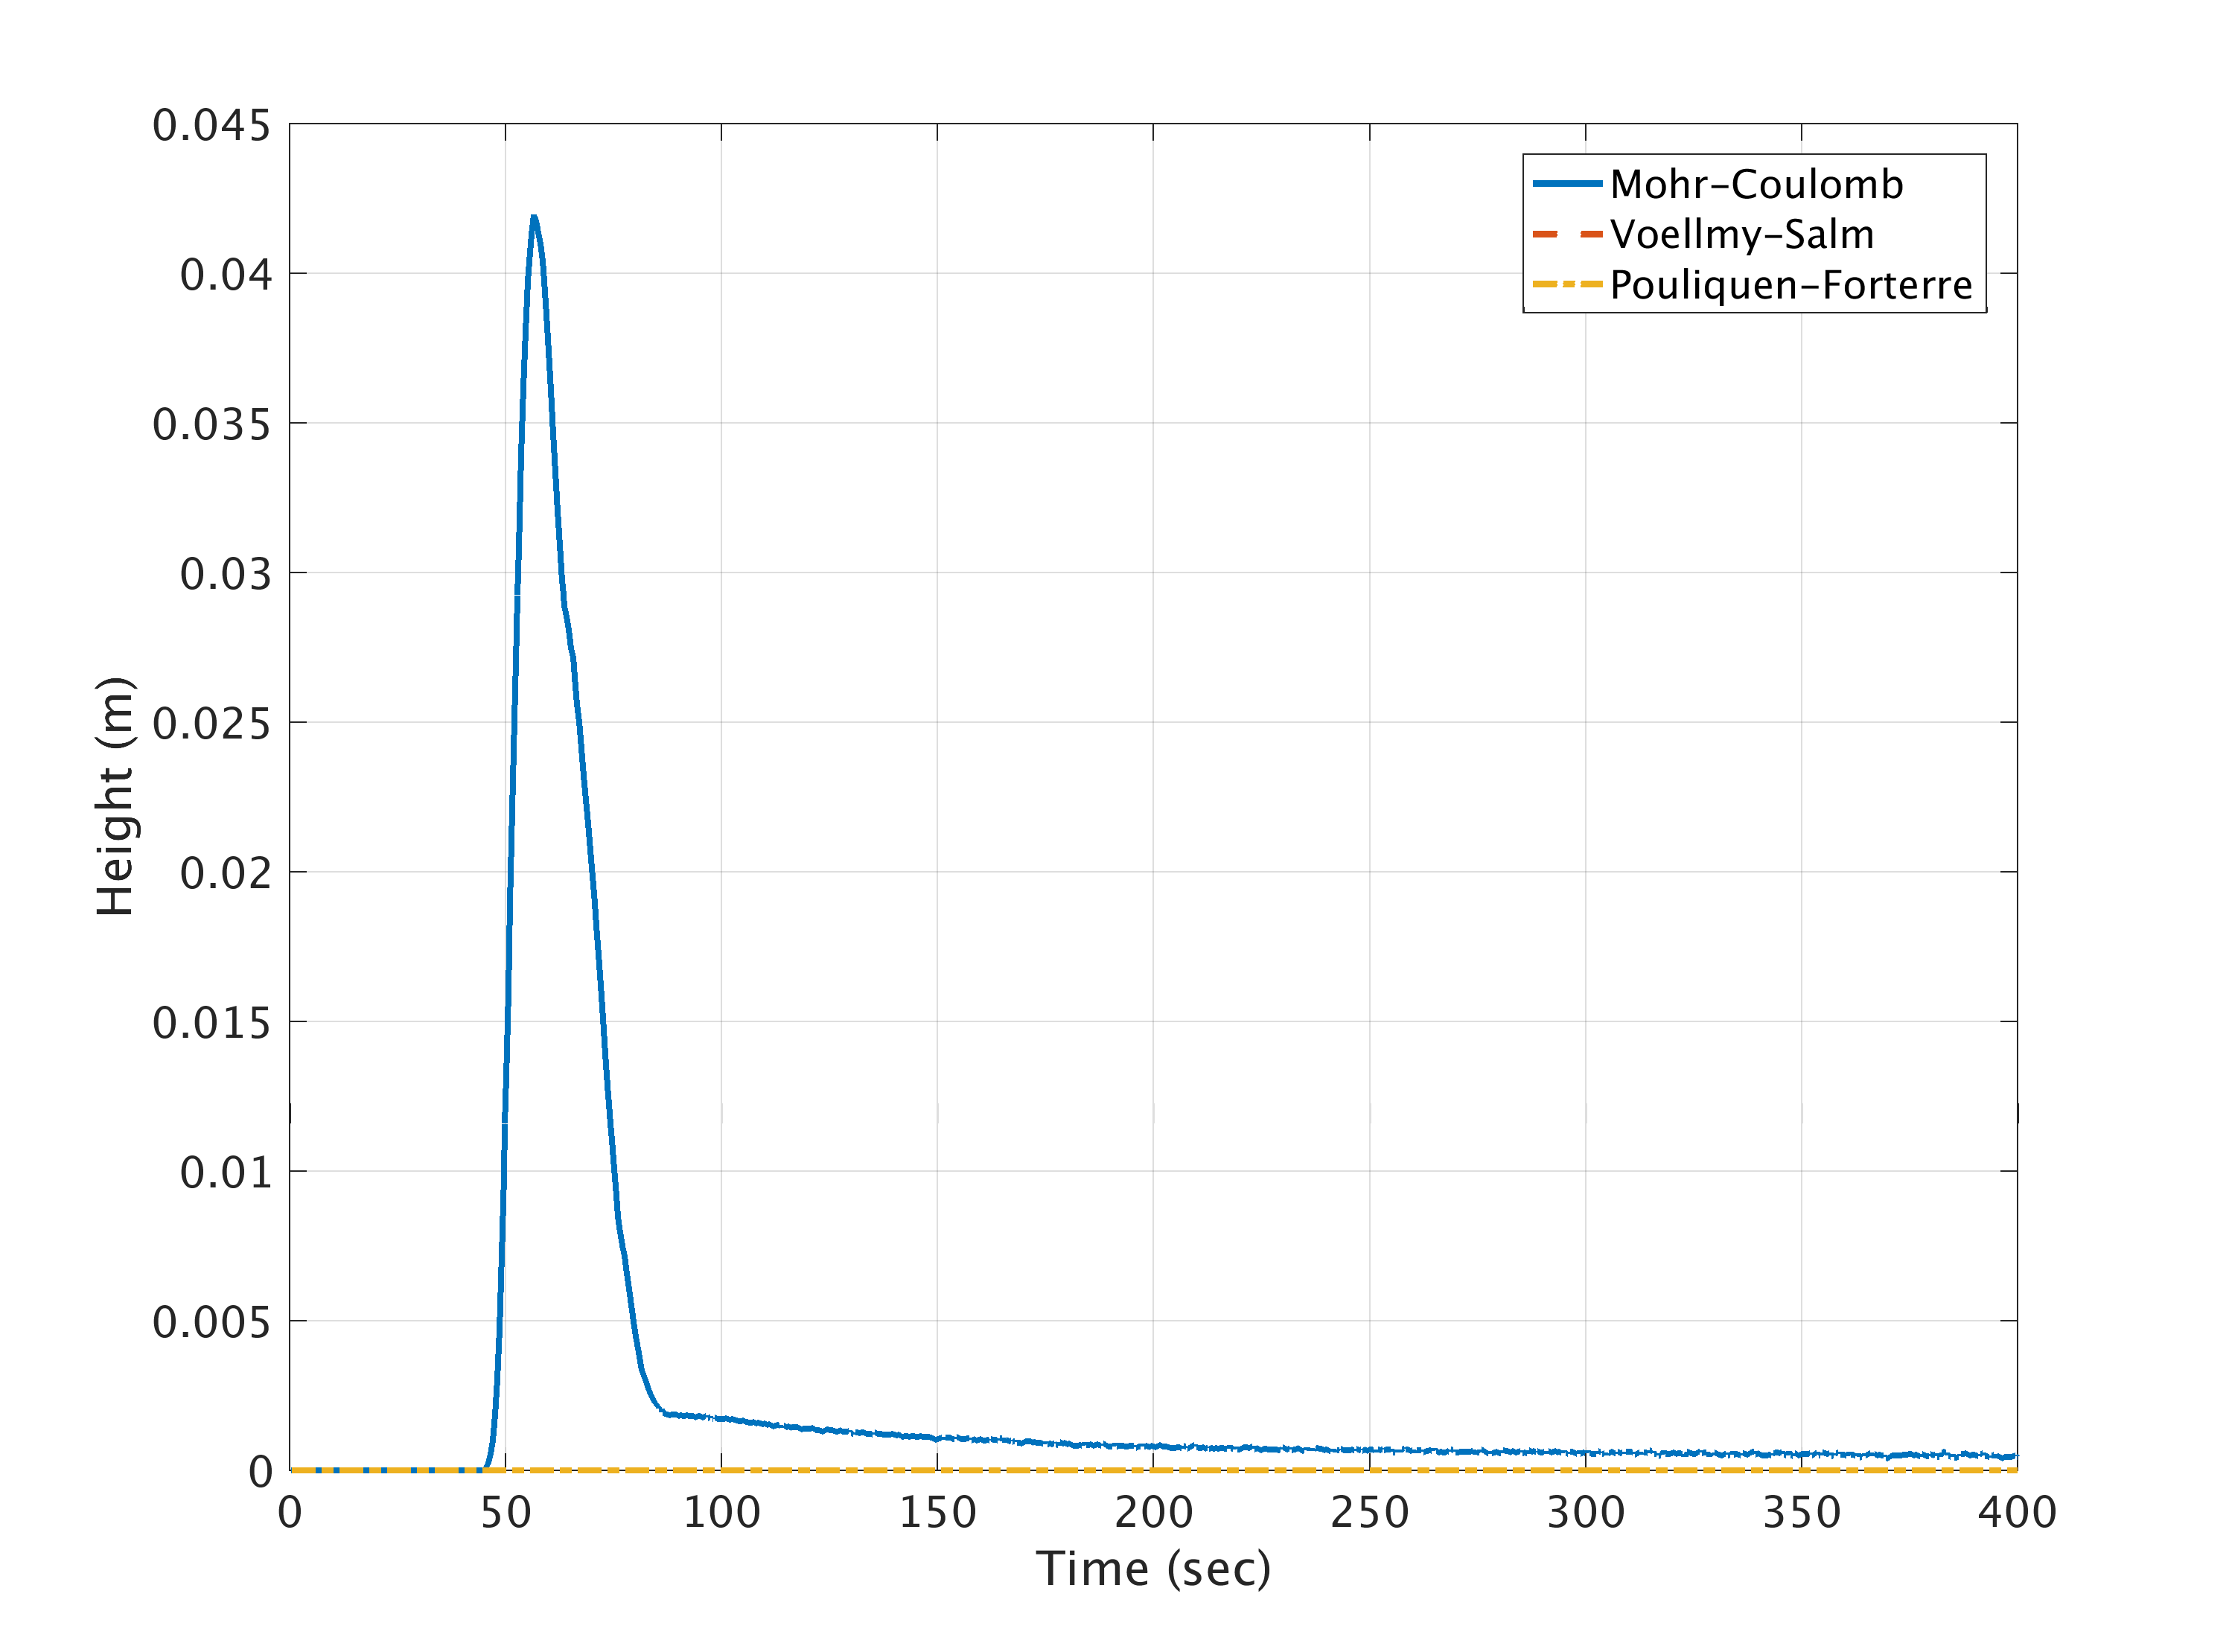
\includegraphics[width=1\textwidth]{HeightMeans/H11All.png}     
        \subcaption{Flow Height Records, Location 11.}
        \label{fig:MFHR_L11}
	\end{minipage}
	\begin{minipage}[b]{0.5\linewidth}
	\centering
    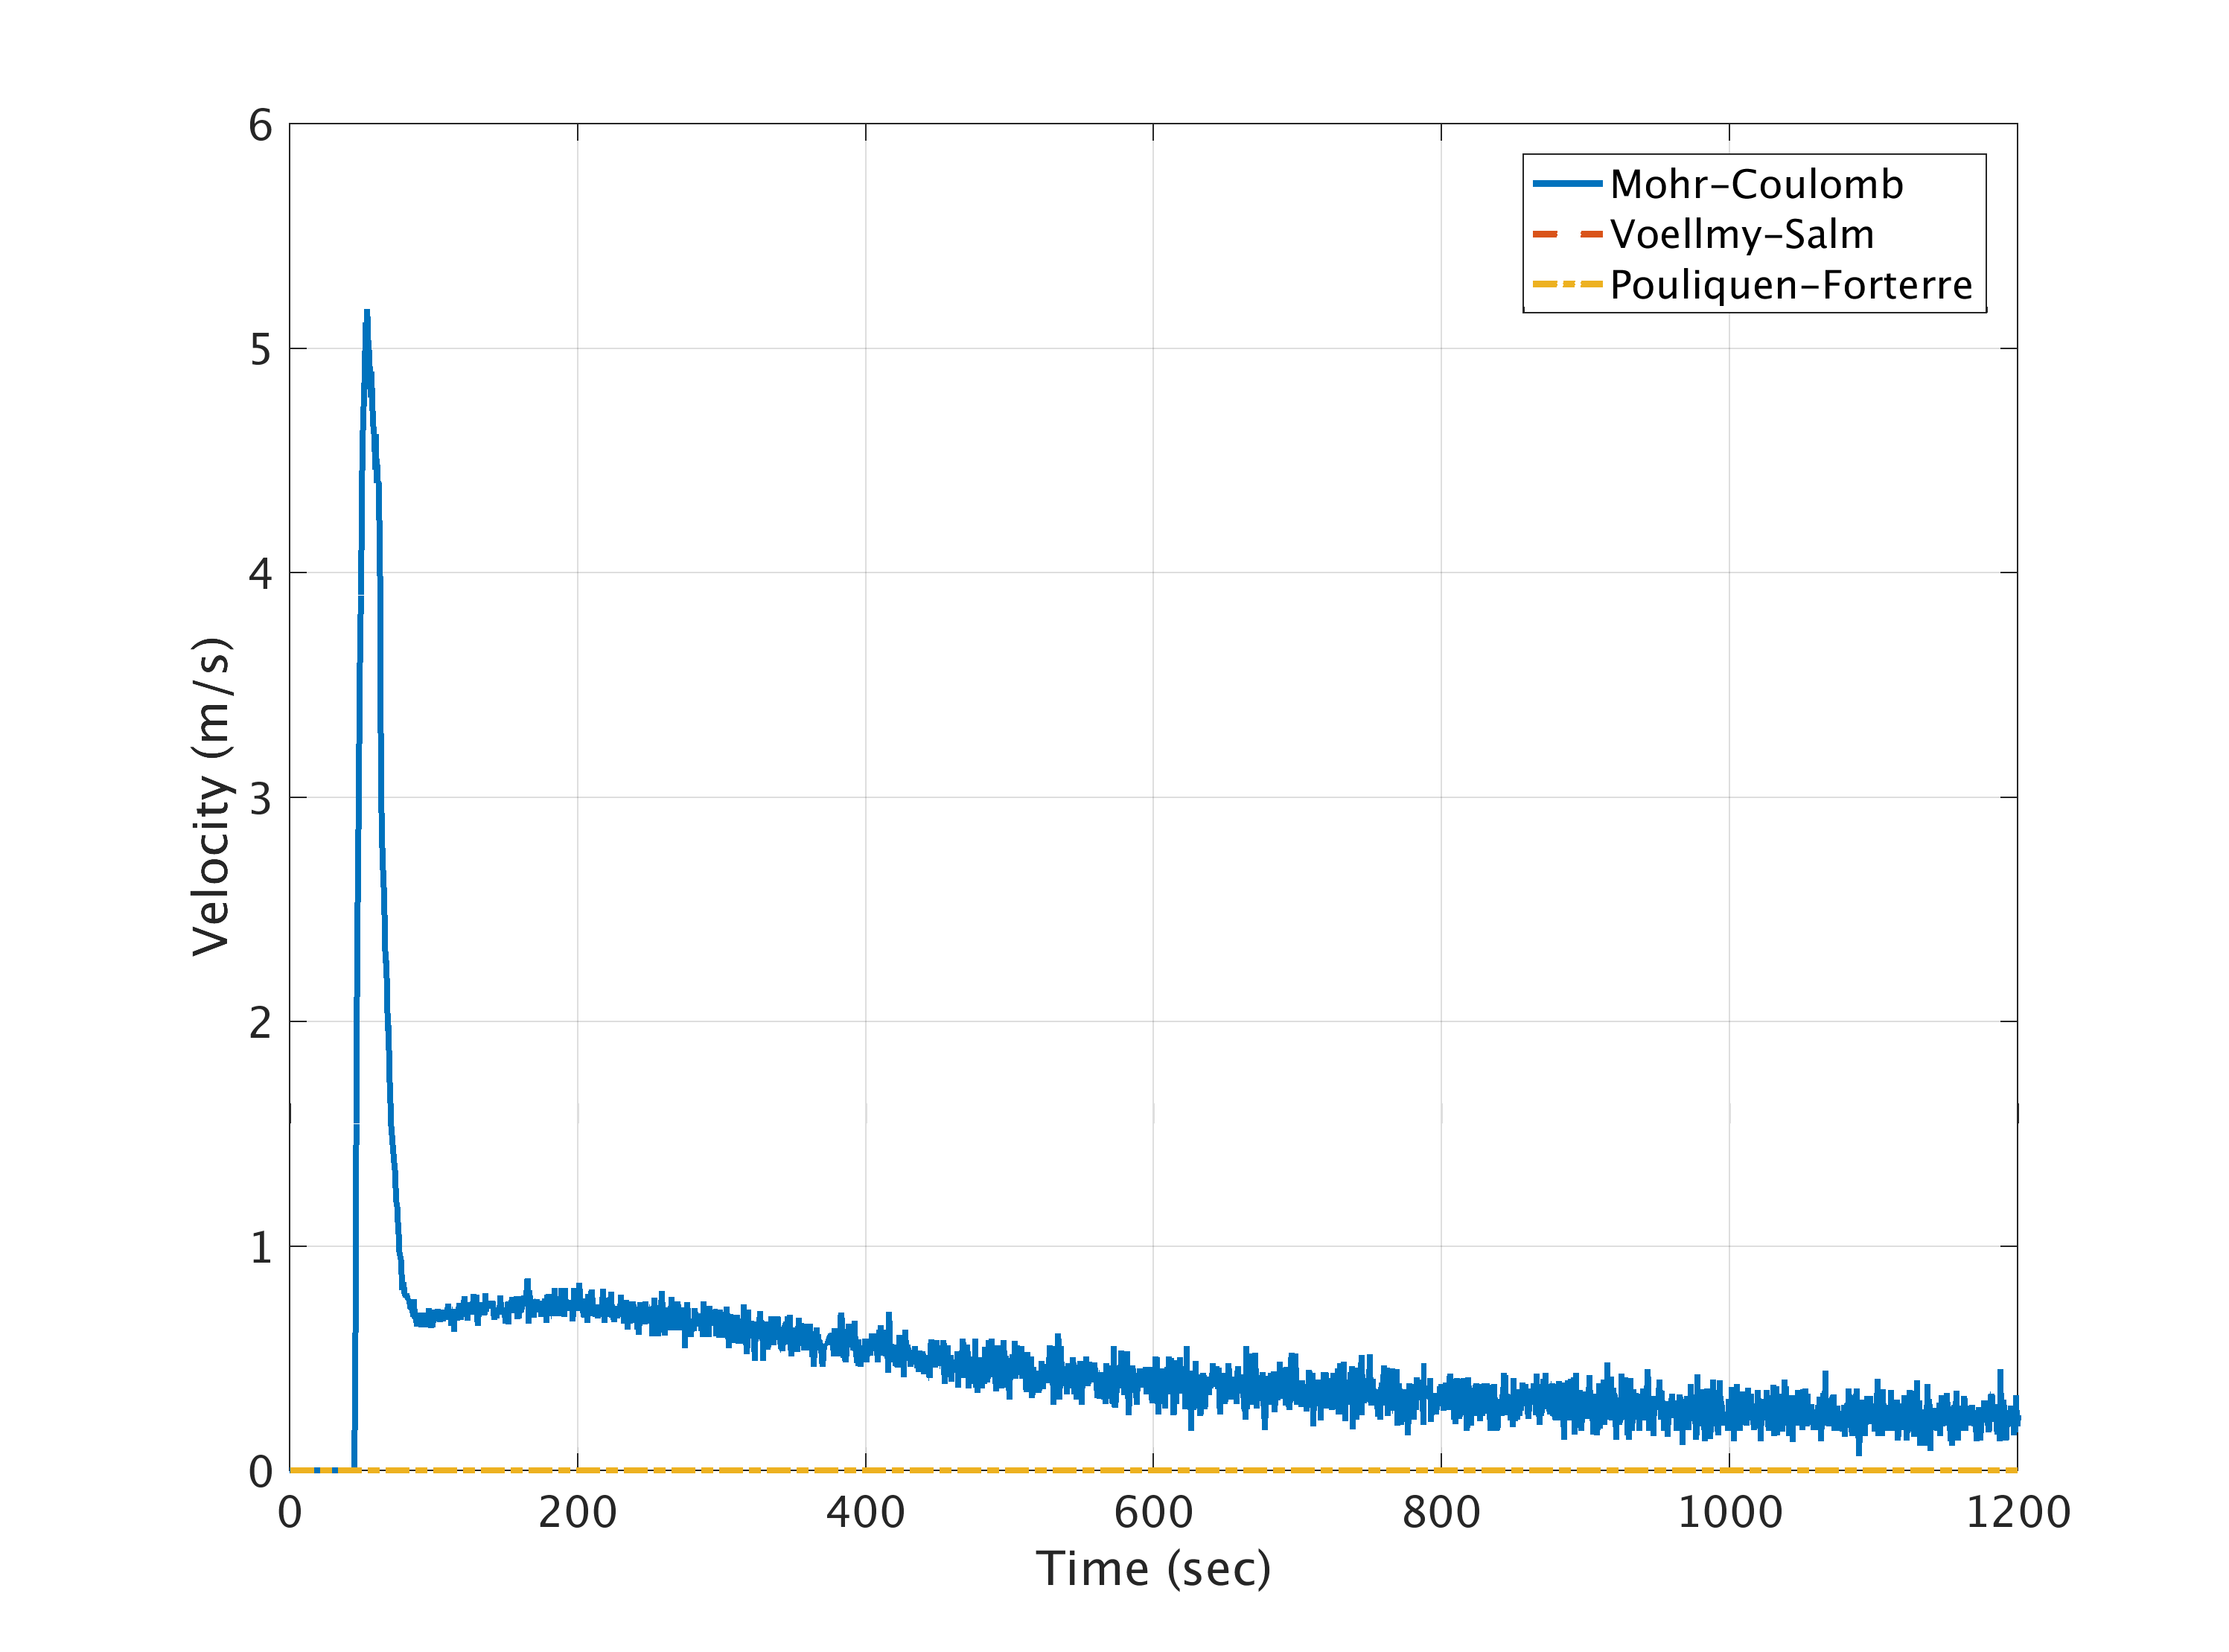
\includegraphics[width=1\textwidth]{VelocityMeans/V11All.png}
        \subcaption{Flow Velocity Records, Location 11.}
        \label{fig:MFVR_L11}
	\end{minipage}
	
	\caption{Mean Values of Flow Height and Velocity Records at locations 10 and 11.}\label{fig:MFHVR_L1011}	
\end{figure}

\section{Statistics of Net Force Records}\label{sec:NetF}

\begin{figure}[H]
	\begin{minipage}[b]{0.5\linewidth}
	\centering
    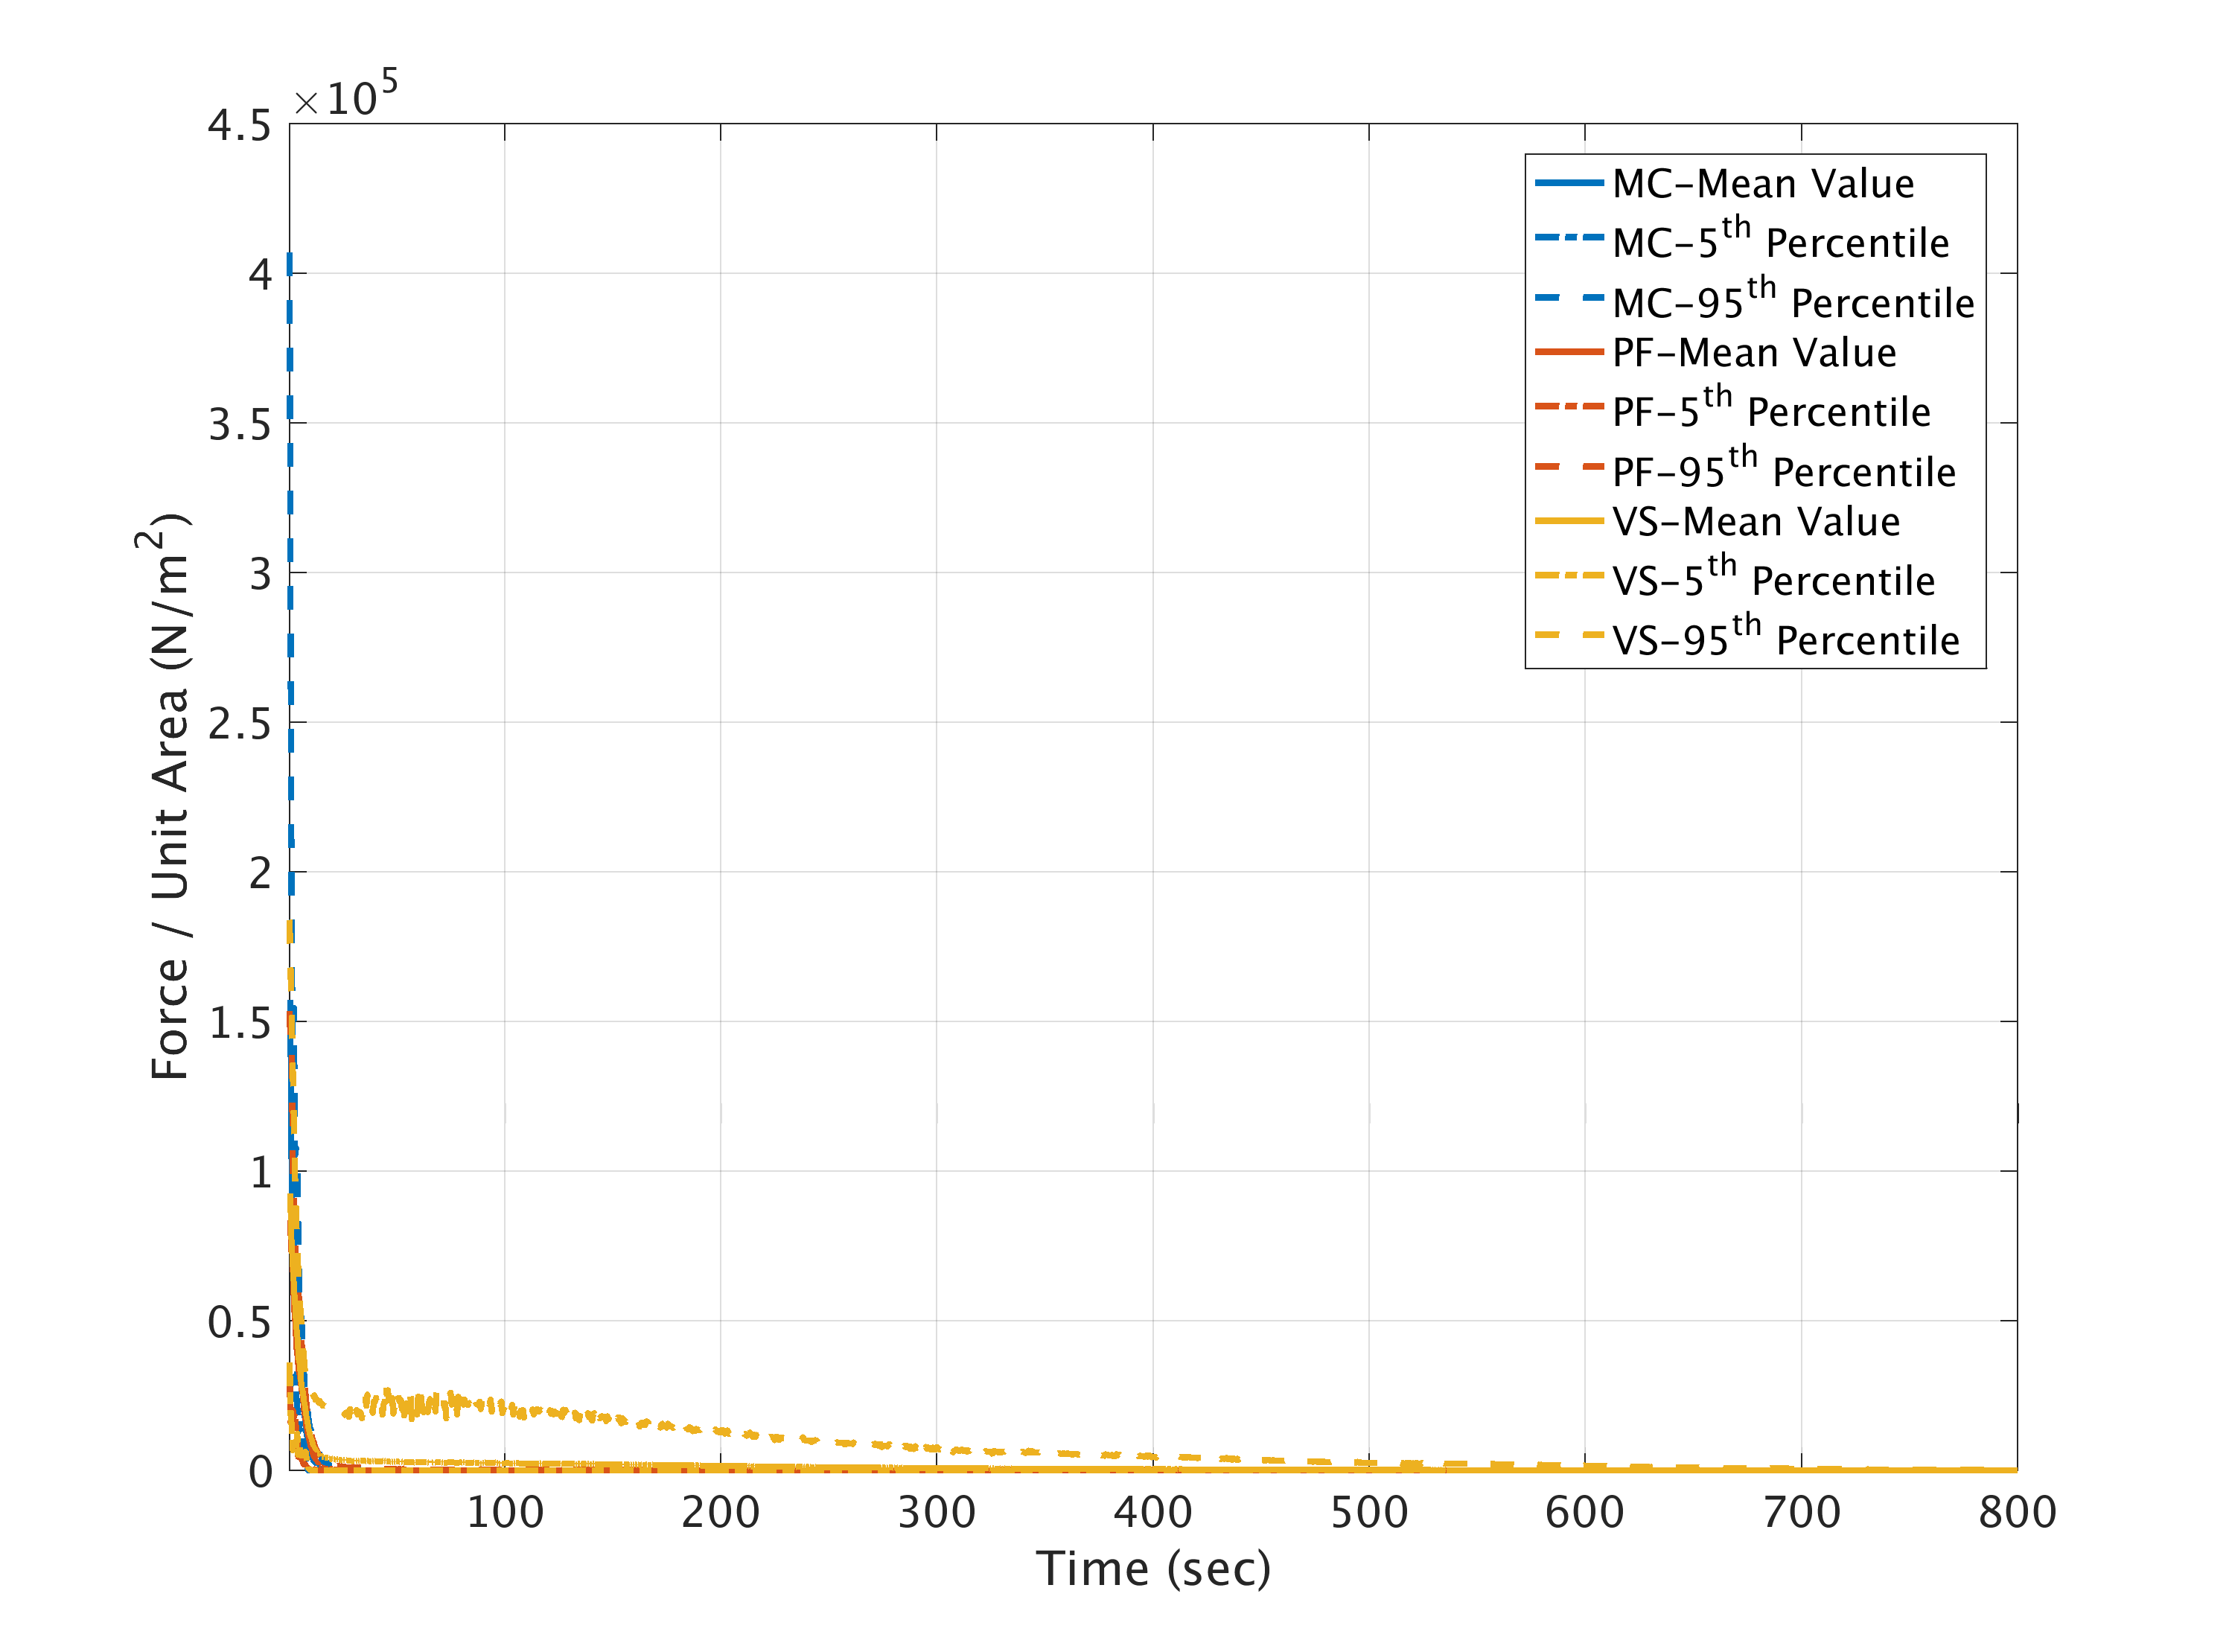
\includegraphics[width=1\textwidth]{NetFAll/NetF1All.png}     
        \subcaption{Net Force Records, Location 1.}
        \label{fig:NF1}
	\end{minipage}
	\begin{minipage}[b]{0.5\linewidth}
	\centering
    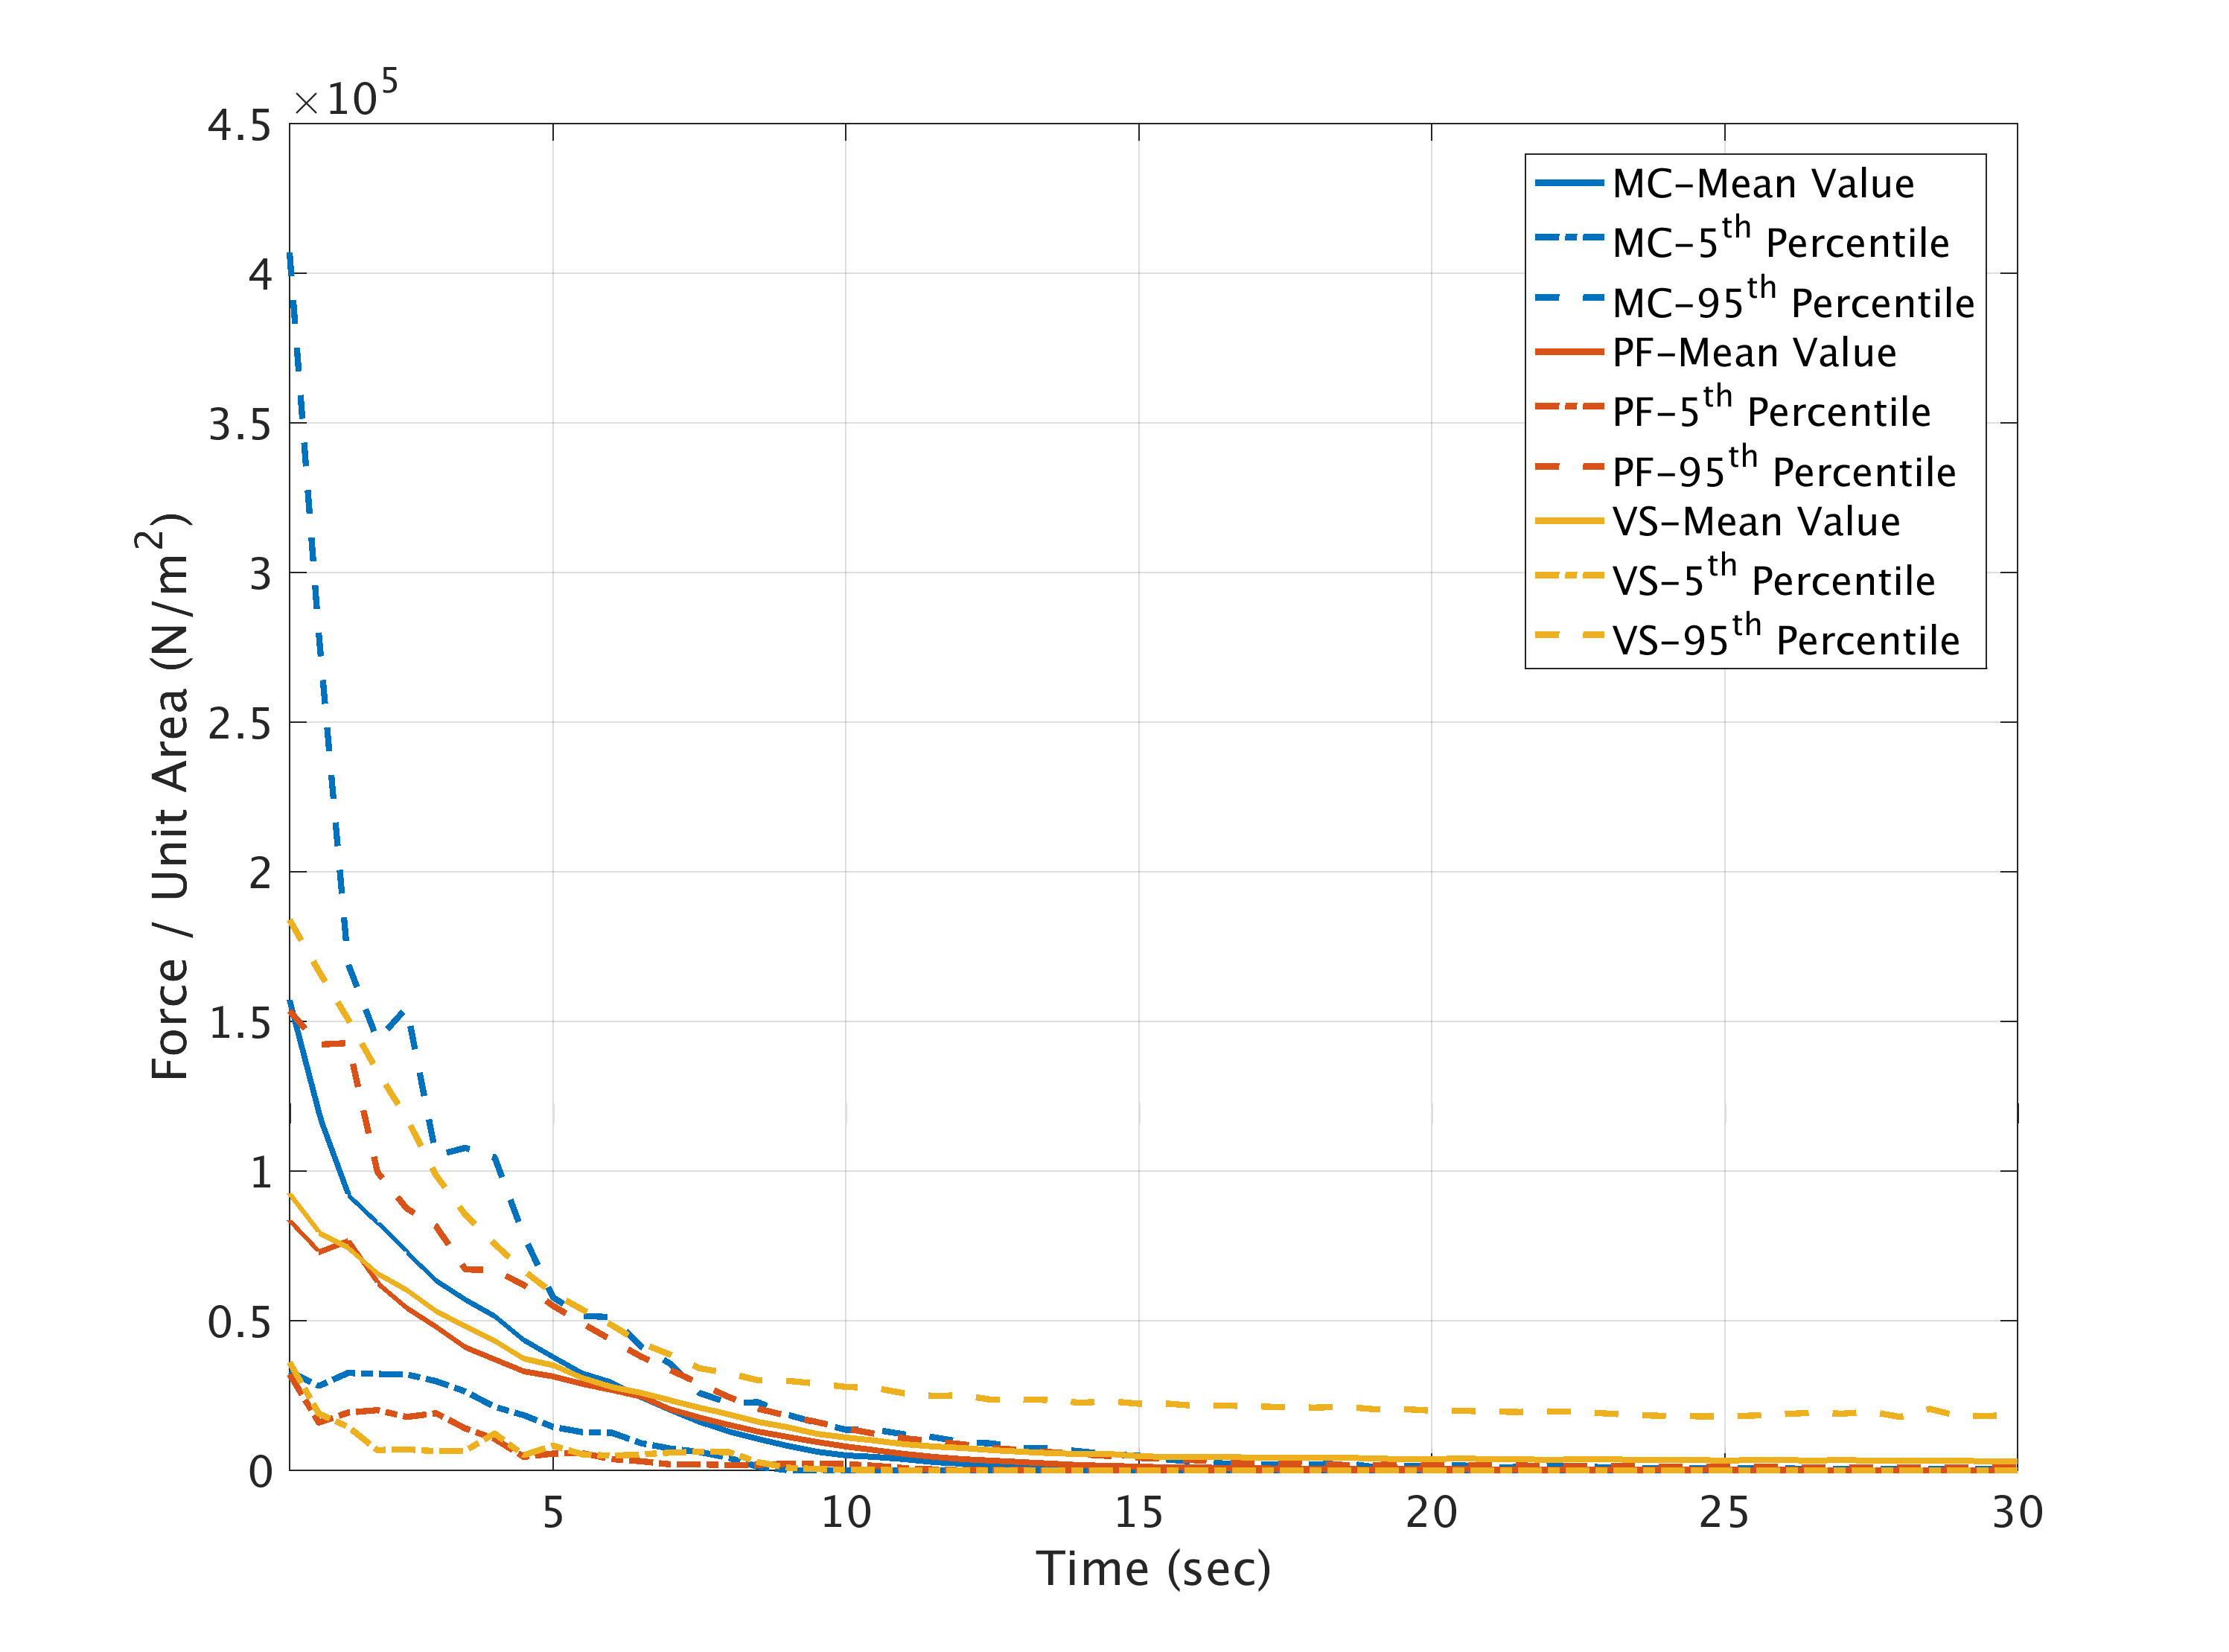
\includegraphics[width=1\textwidth]{NetFAll/NetF1All_z.png}
        \subcaption{Zoomed view of Fig. (\ref{fig:NF1}).}
        \label{fig:NF1zoom}
	\end{minipage}
	
	\begin{minipage}[b]{0.5\linewidth}
	\centering
    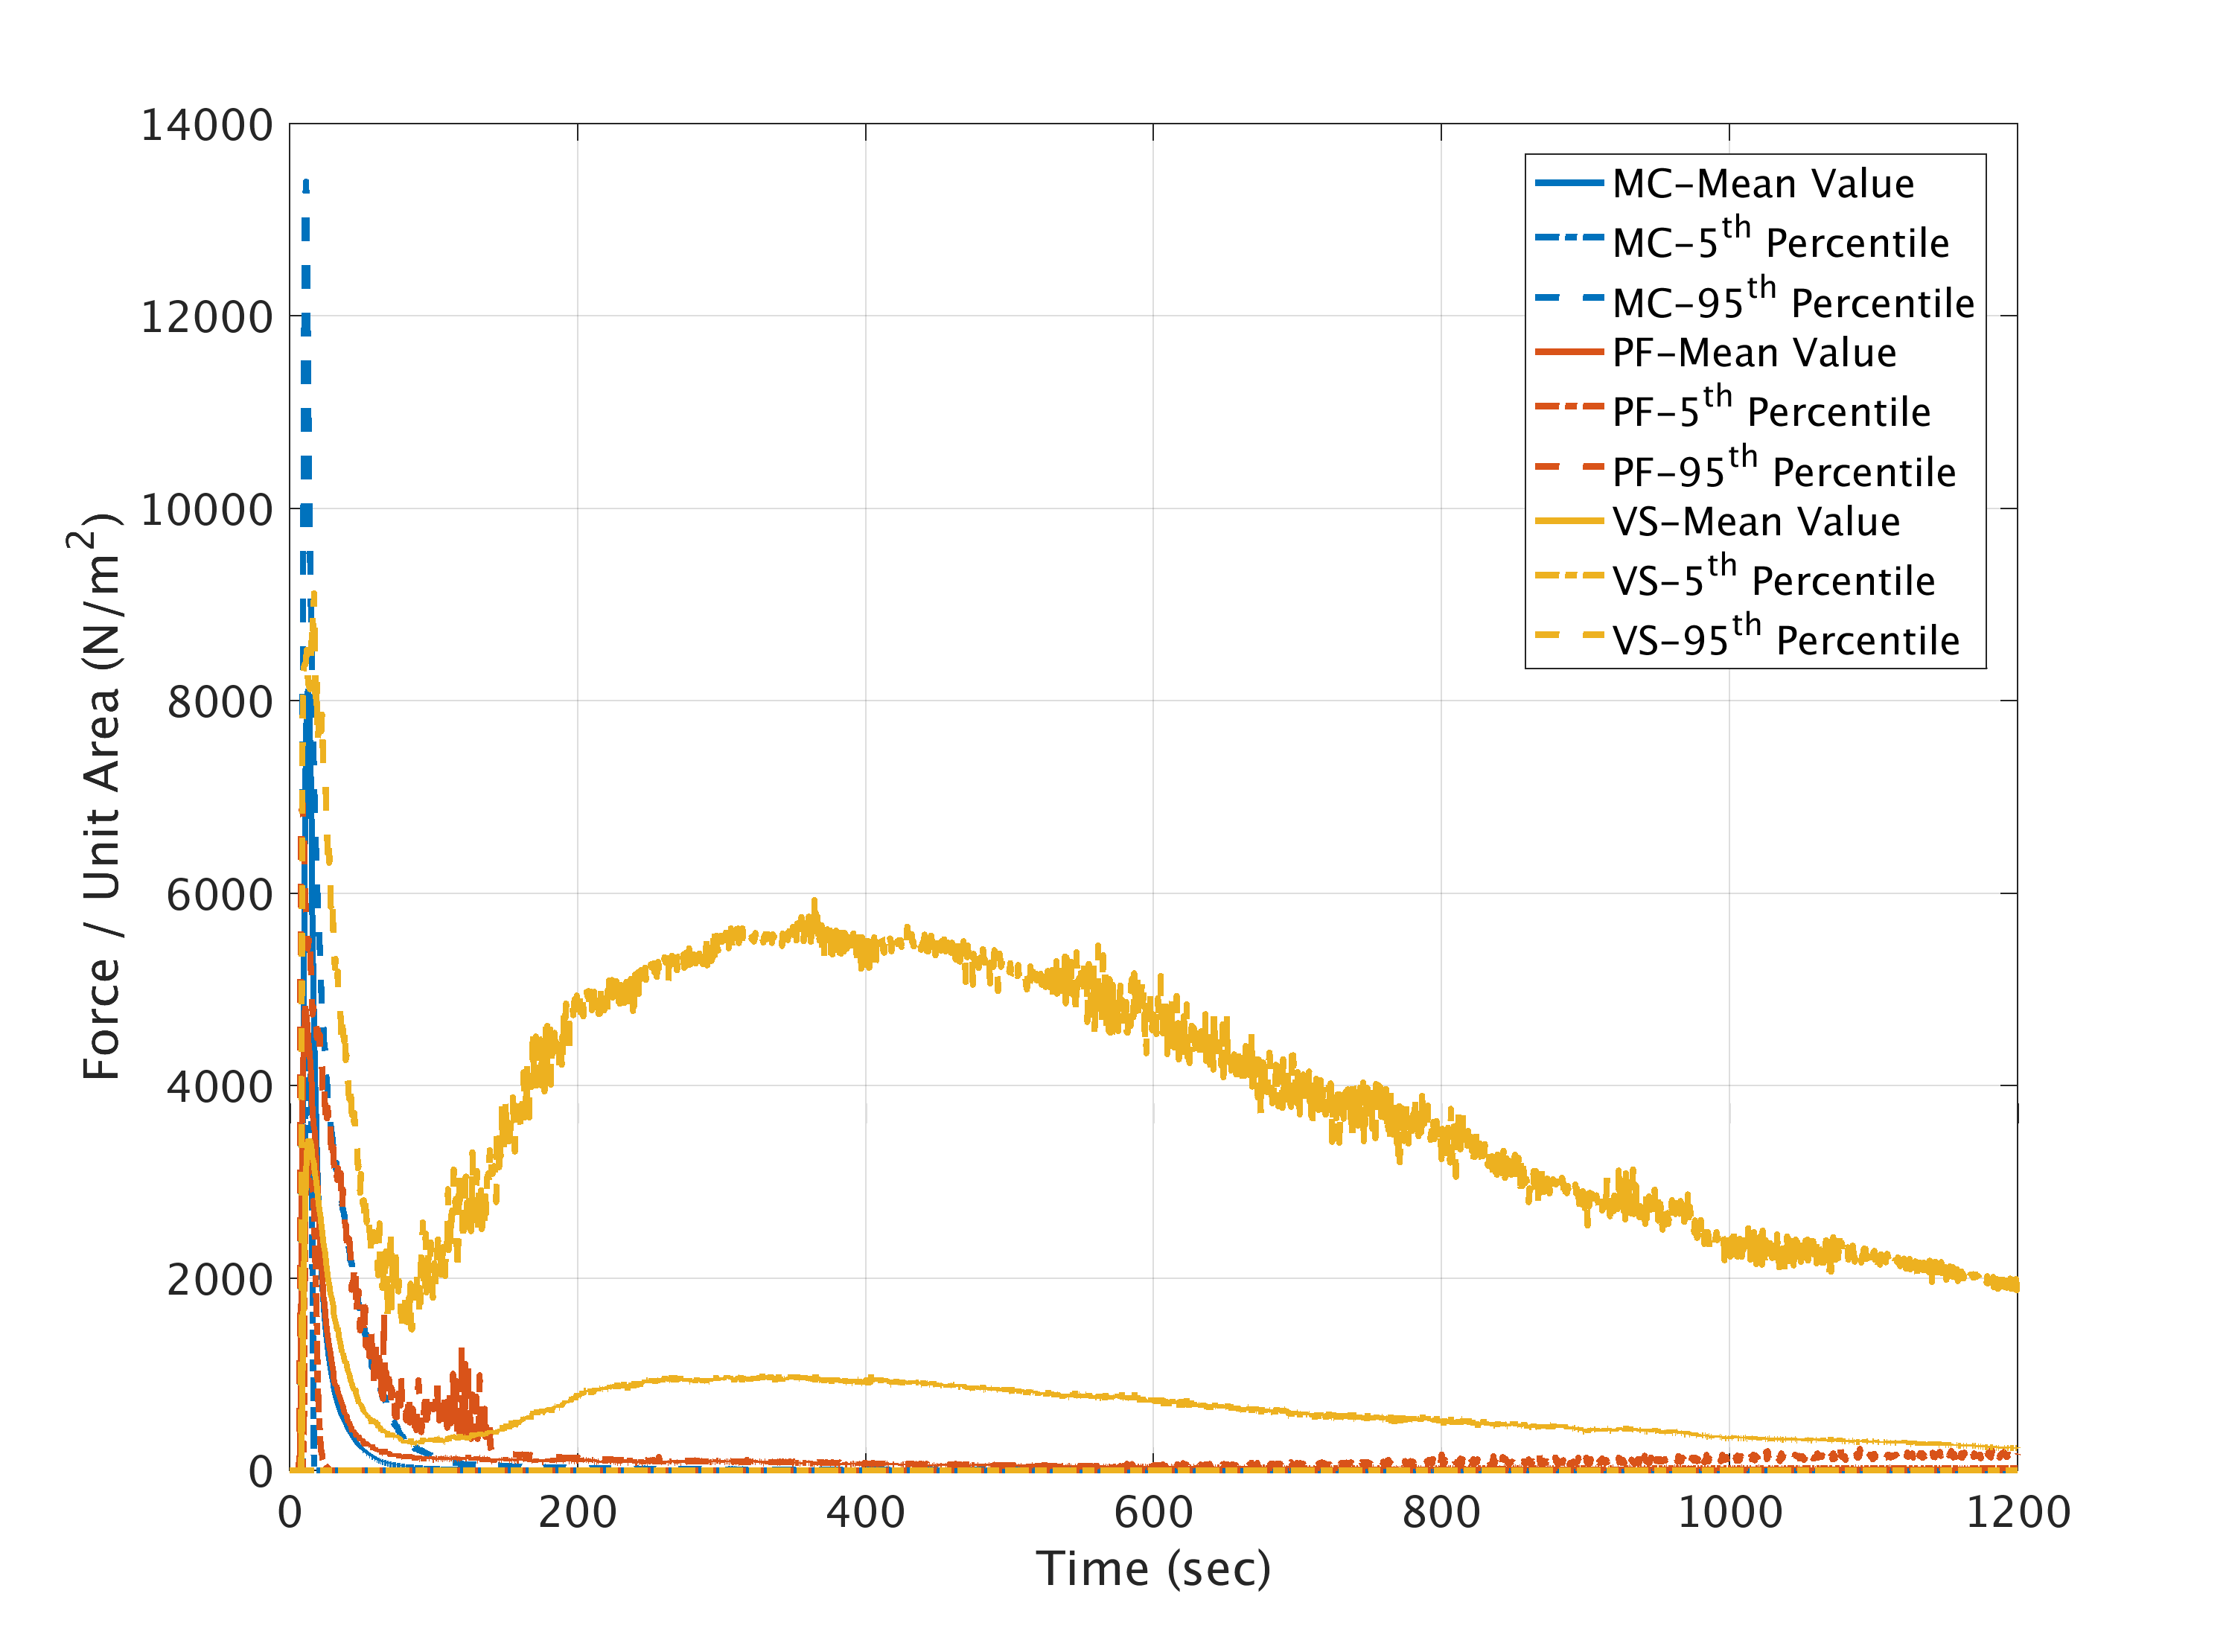
\includegraphics[width=1\textwidth]{NetFAll/NetF2All.png}     
        \subcaption{Net Force Records, Location 2.}
        \label{fig:NF2}
	\end{minipage}
	\begin{minipage}[b]{0.5\linewidth}
	\centering
    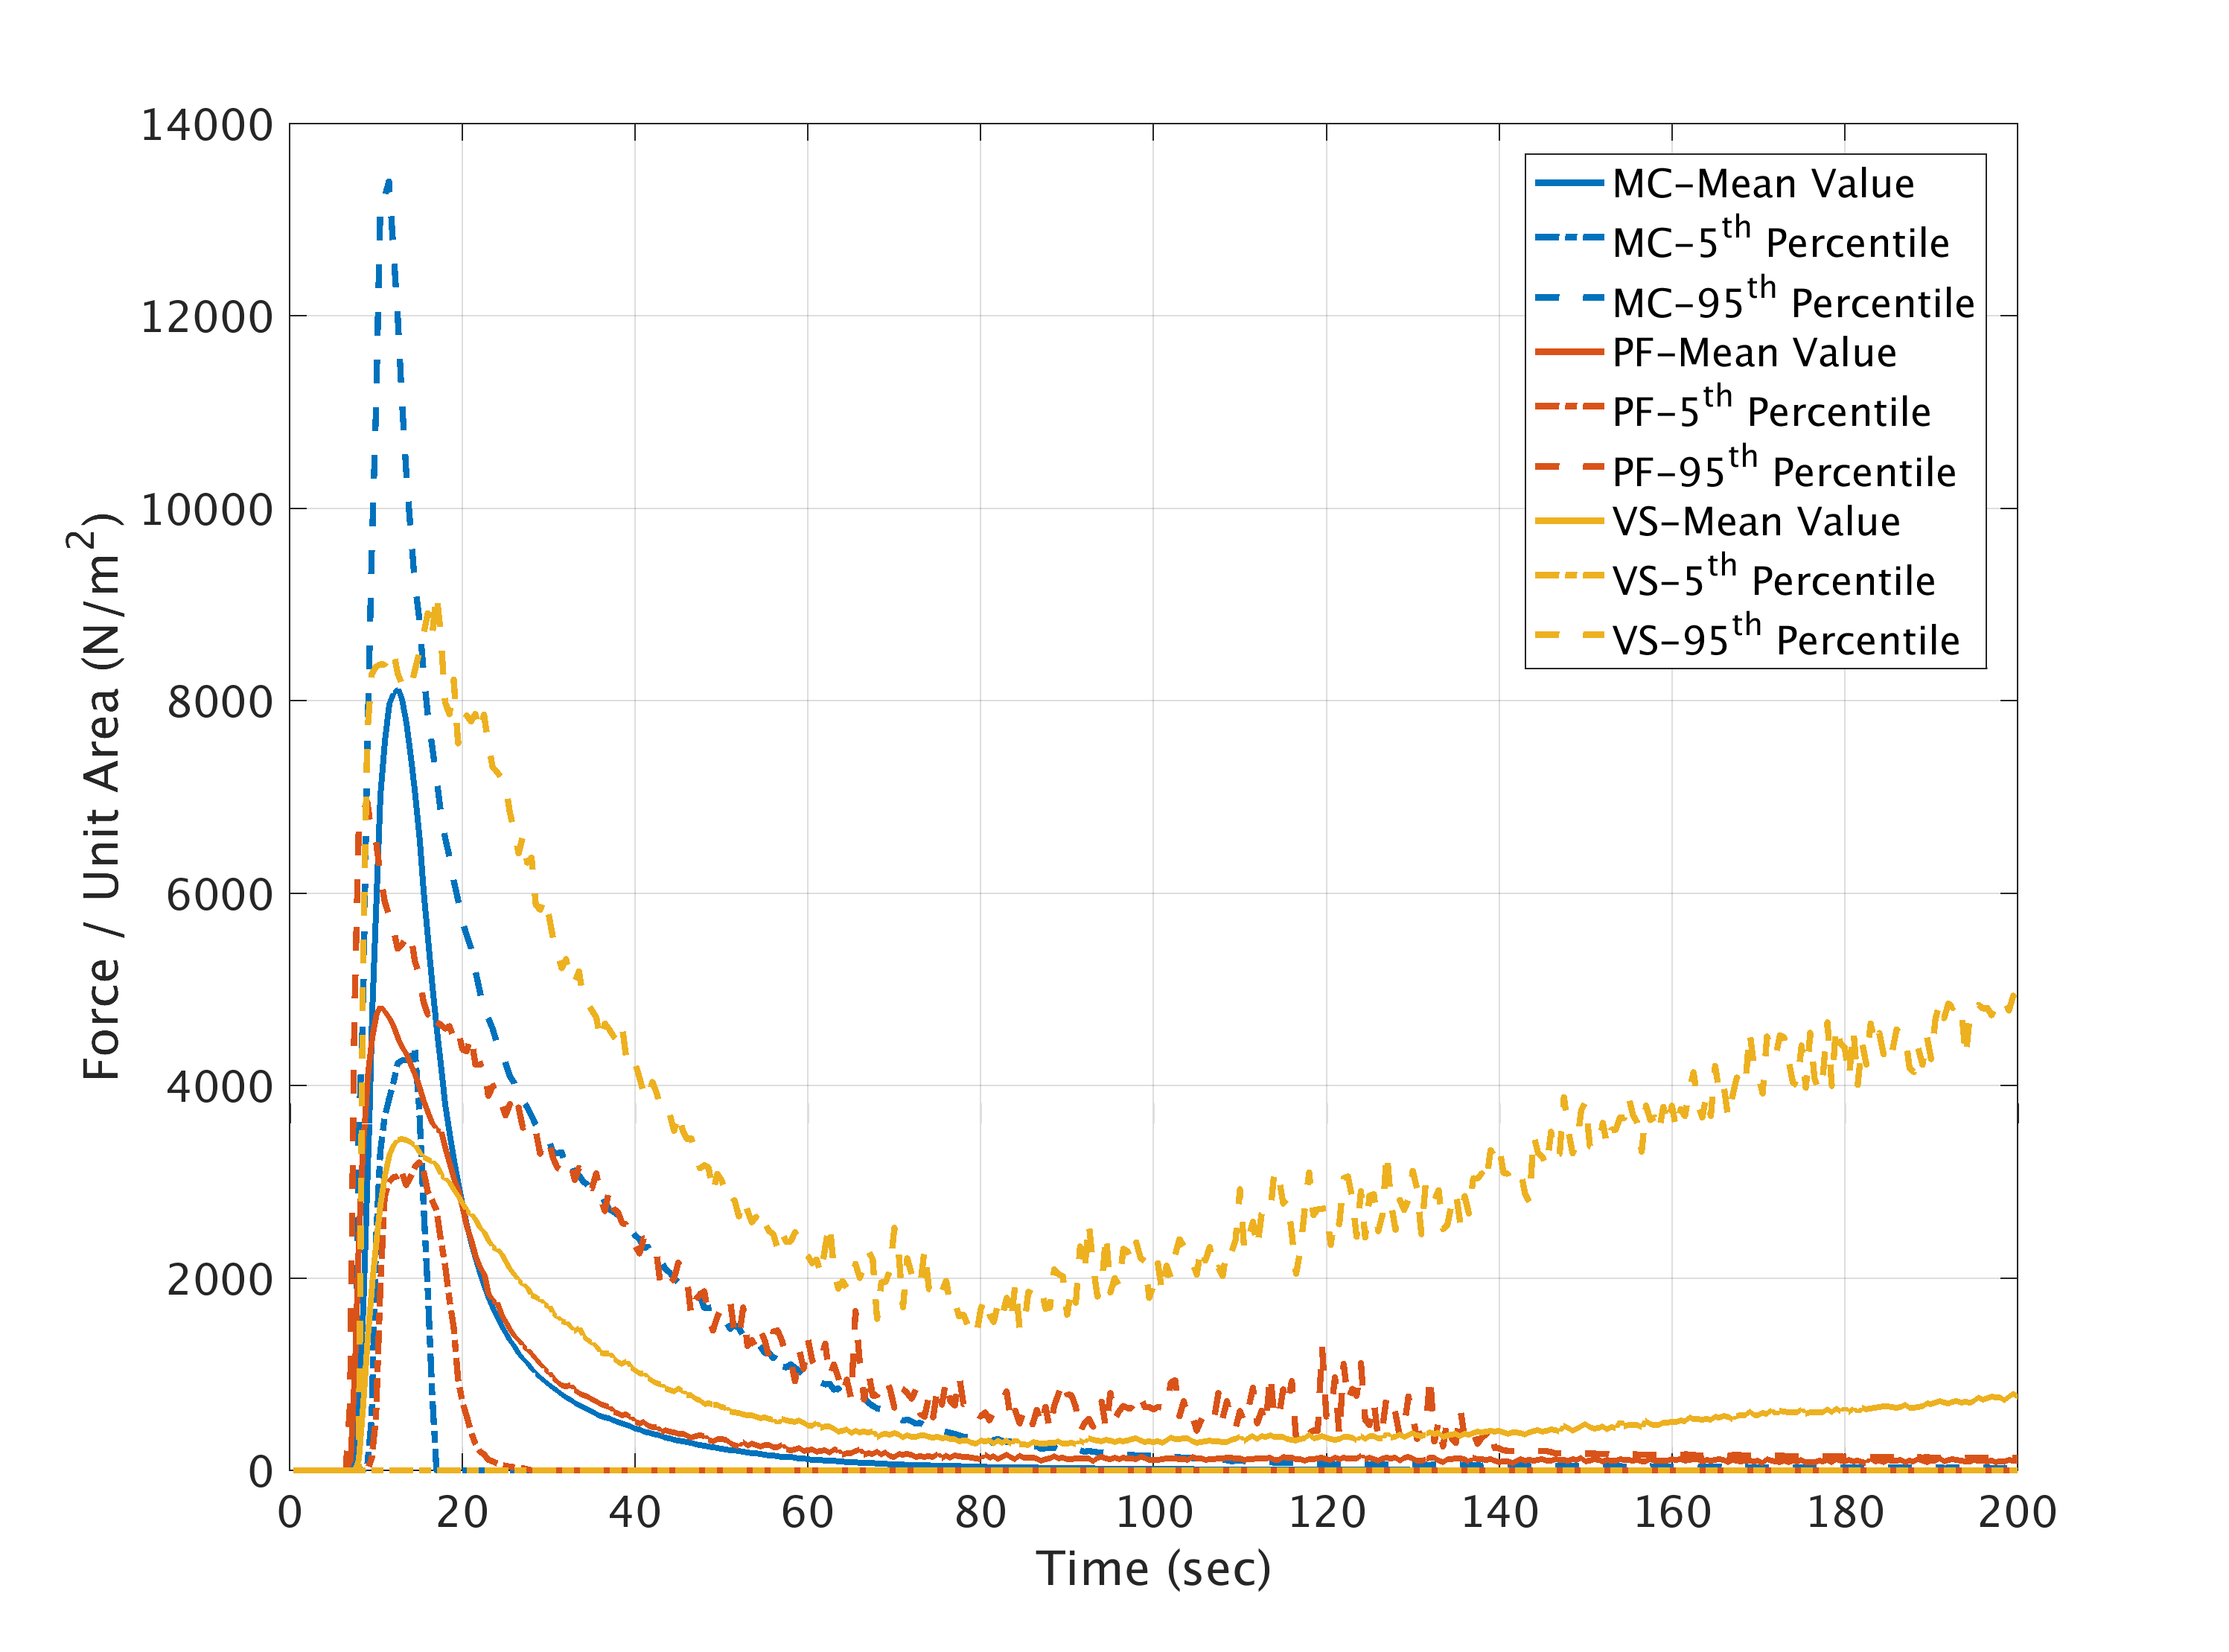
\includegraphics[width=1\textwidth]{NetFAll/NetF2All_z.png}
        \subcaption{Zoomed view of Fig. (\ref{fig:NF2}).}
        \label{fig:NF2zoom}
	\end{minipage}
	
	\begin{minipage}[b]{0.5\linewidth}
	\centering
    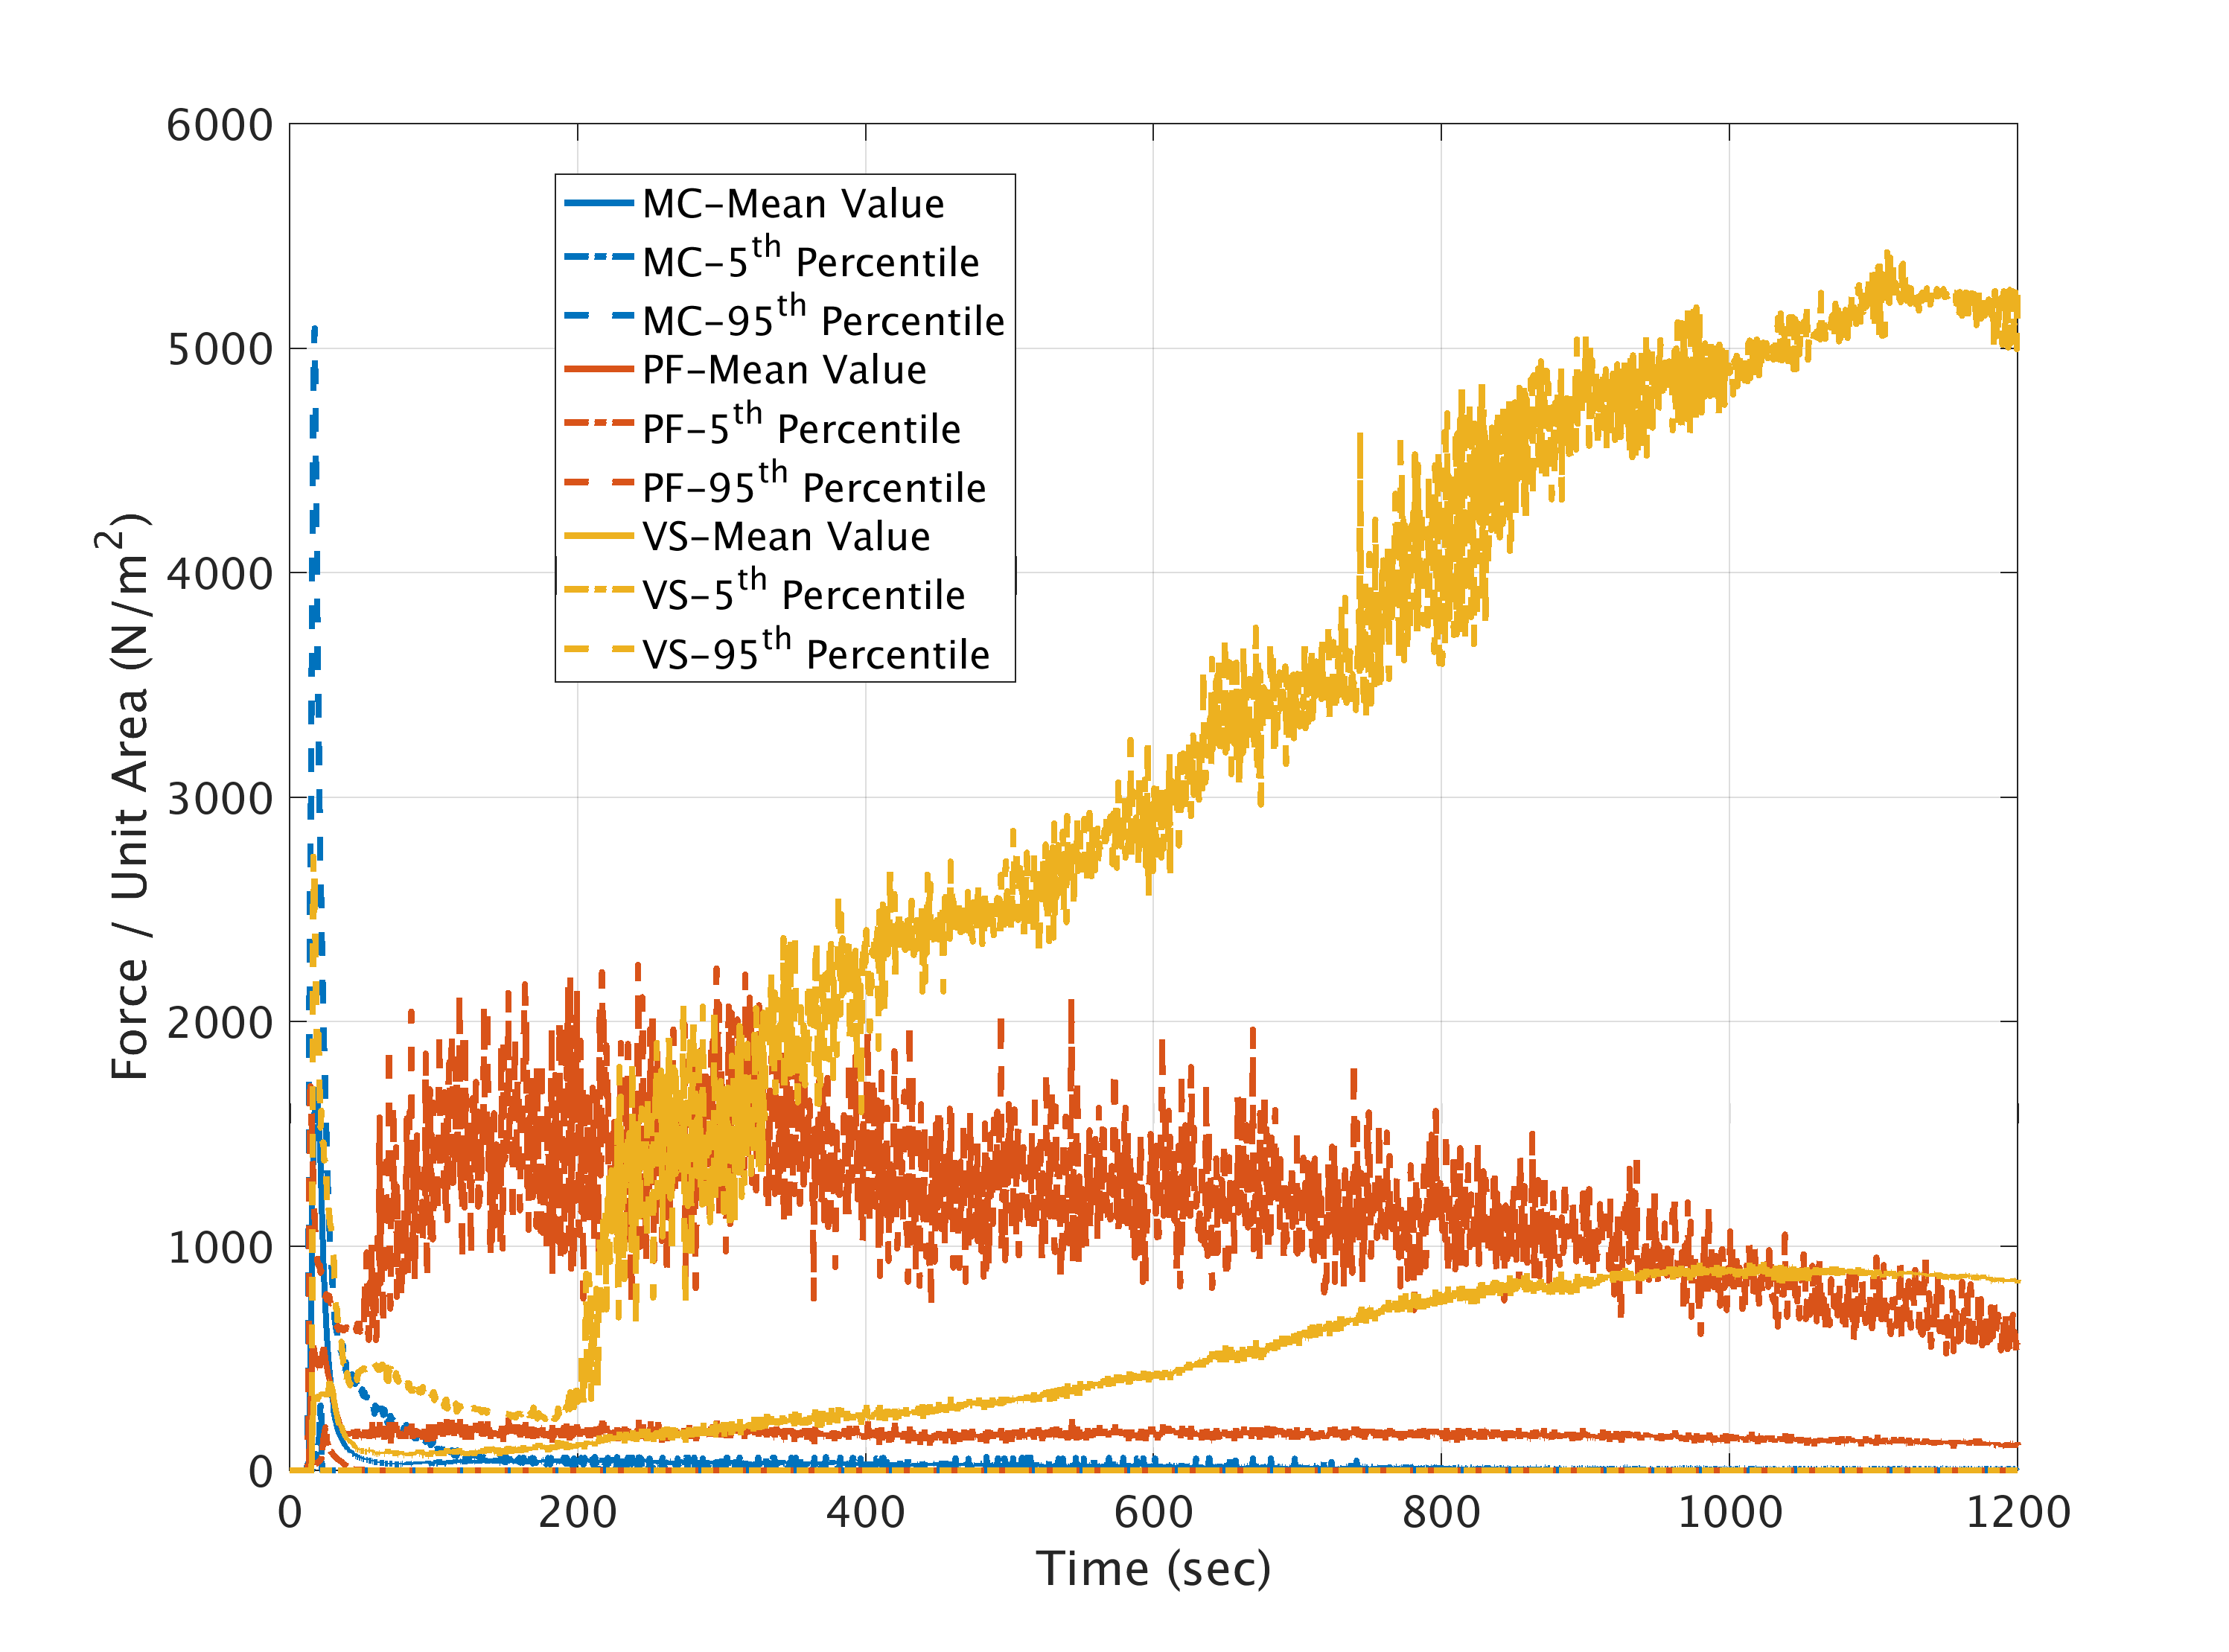
\includegraphics[width=1\textwidth]{NetFAll/NetF3All.png}     
        \subcaption{Net Force Records, Location3 .}
        \label{fig:NF3}
	\end{minipage}
	\begin{minipage}[b]{0.5\linewidth}
	\centering
    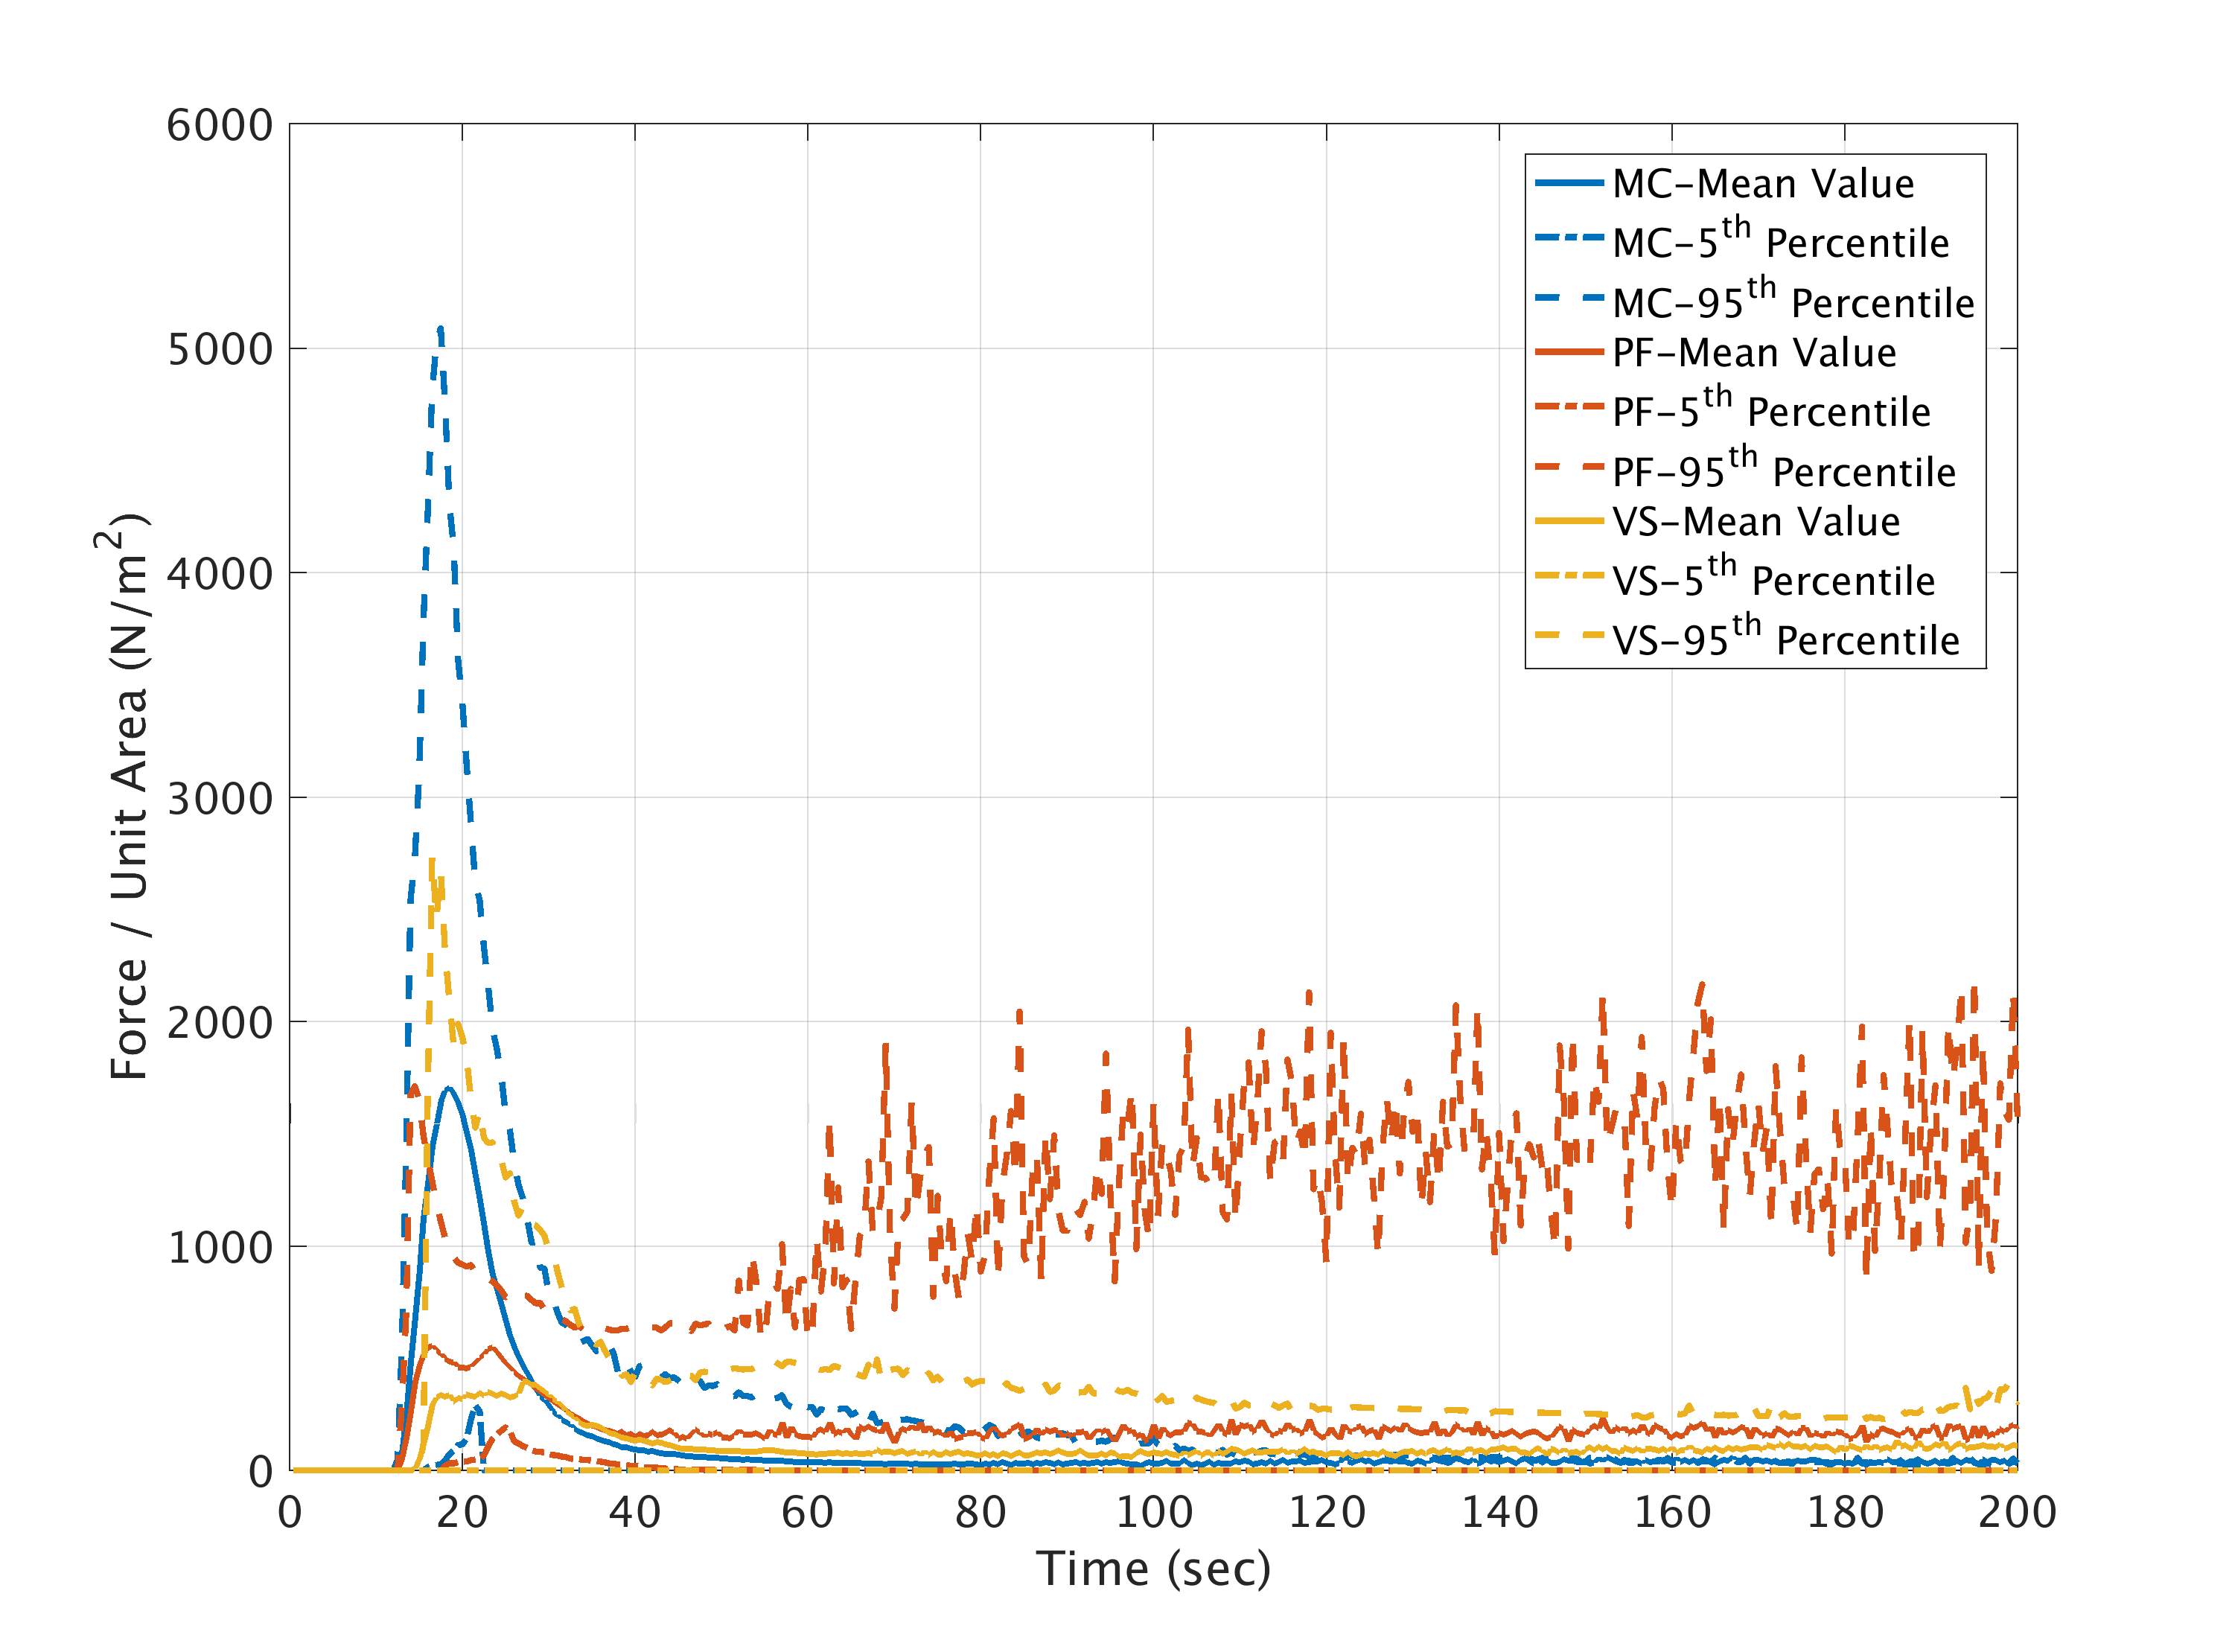
\includegraphics[width=1\textwidth]{NetFAll/NetF3All_z.png}
        \subcaption{Zoomed view of Fig. (\ref{fig:NF3}).}
        \label{fig:NF3zoom}
	\end{minipage}
	
	\caption{Mean Values, $5^{\mathrm{th}}$ and $95^{\mathrm{th}}$ percentile records of Net Force at locations 1, 2 and 3.}\label{fig:NF123}	
\end{figure}

\begin{figure}[H]
	\begin{minipage}[b]{0.5\linewidth}
	\centering
    \includegraphics[width=1\textwidth]{NetFAll/NetF4All.png}     
        \subcaption{Net Force Records, Location 4.}
        \label{fig:NF4}
	\end{minipage}
	\begin{minipage}[b]{0.5\linewidth}
	\centering
    \includegraphics[width=1\textwidth]{NetFAll/NetF4All_z.png}
        \subcaption{Zoomed view of Fig. (\ref{fig:NF4}).}
        \label{fig:NF4zoom}
	\end{minipage}
	
	\begin{minipage}[b]{0.5\linewidth}
	\centering
    \includegraphics[width=1\textwidth]{NetFAll/NetF5All.png}     
        \subcaption{Net Force Records, Location 5.}
        \label{fig:NF5}
	\end{minipage}
	\begin{minipage}[b]{0.5\linewidth}
	\centering
    \includegraphics[width=1\textwidth]{NetFAll/NetF5All_z.png}
        \subcaption{Zoomed view of Fig. (\ref{fig:NF5}).}
        \label{fig:NF5zoom}
	\end{minipage}
	
	\begin{minipage}[b]{0.5\linewidth}
	\centering
    \includegraphics[width=1\textwidth]{NetFAll/NetF6All.png}     
        \subcaption{Net Force Records, Location 6.}
        \label{fig:NF6}
	\end{minipage}
	\begin{minipage}[b]{0.5\linewidth}
	\centering
    \includegraphics[width=1\textwidth]{NetFAll/NetF6All_z.png}
        \subcaption{Zoomed view of Fig. (\ref{fig:NF6}).}
        \label{fig:NF6zoom}
	\end{minipage}
	
	\caption{Mean Values, $5^{\mathrm{th}}$ and $95^{\mathrm{th}}$ percentile records of Net Force at locations 4, 5 and 6.}\label{fig:NF456}	
\end{figure}

\begin{figure}[H]
	\begin{minipage}[b]{0.5\linewidth}
	\centering
    \includegraphics[width=1\textwidth]{NetFAll/NetF7All.png}     
        \subcaption{Net Force Records, Location 7.}
        \label{fig:NF7}
	\end{minipage}
	\begin{minipage}[b]{0.5\linewidth}
	\centering
    \includegraphics[width=1\textwidth]{NetFAll/NetF7All_z.png}
        \subcaption{Zoomed view of Fig. (\ref{fig:NF7}).}
        \label{fig:NF7zoom}
	\end{minipage}
	
	\begin{minipage}[b]{0.5\linewidth}
	\centering
    \includegraphics[width=1\textwidth]{NetFAll/NetF8All.png}     
        \subcaption{Net Force Records, Location 8.}
        \label{fig:NF8}
	\end{minipage}
	\begin{minipage}[b]{0.5\linewidth}
	\centering
    \includegraphics[width=1\textwidth]{NetFAll/NetF8All_z.png}
        \subcaption{Zoomed view of Fig. (\ref{fig:NF8}).}
        \label{fig:NF8zoom}
	\end{minipage}
	
	\begin{minipage}[b]{0.5\linewidth}
	\centering
    \includegraphics[width=1\textwidth]{NetFAll/NetF9All.png}     
        \subcaption{Net Force Records, Location 9.}
        \label{fig:NF9}
	\end{minipage}
	\begin{minipage}[b]{0.5\linewidth}
	\centering
    \includegraphics[width=1\textwidth]{NetFAll/NetF9All_z.png}
        \subcaption{Zoomed view of Fig. (\ref{fig:NF9}).}
        \label{fig:NF9zoom}
	\end{minipage}
	
	\caption{Mean Values, $5^{\mathrm{th}}$ and $95^{\mathrm{th}}$ percentile records of Net Force at locations 7, 8 and 9.}\label{fig:NF789}	
\end{figure}

\begin{figure}[H]
	\begin{minipage}[b]{0.5\linewidth}
	\centering
    \includegraphics[width=1\textwidth]{NetFAll/NetF10All.png}     
        \subcaption{Net Force Records, Location 10.}
        \label{fig:NF10}
	\end{minipage}
	\begin{minipage}[b]{0.5\linewidth}
	\centering
    \includegraphics[width=1\textwidth]{NetFAll/NetF10All_z.png}
        \subcaption{Zoomed view of Fig. (\ref{fig:NF10}).}
        \label{fig:NF10zoom}
	\end{minipage}
	
	\begin{minipage}[b]{0.5\linewidth}
	\centering
    \includegraphics[width=1\textwidth]{NetFAll/NetF11All.png}     
        \subcaption{Net Force Records, Location 11.}
        \label{fig:NF11}
	\end{minipage}
	\begin{minipage}[b]{0.5\linewidth}
	\centering
    \includegraphics[width=1\textwidth]{NetFAll/NetF11All_z.png}
        \subcaption{Zoomed view of Fig. (\ref{fig:NF11}).}
        \label{fig:NF11zoom}
	\end{minipage}
	
	\caption{Mean Values, $5^{\mathrm{th}}$ and $95^{\mathrm{th}}$ percentile records of Net Force at locations 10 and 11.}\label{fig:NF1011}	
\end{figure}

\bibliographystyle{unsrt}
\bibliography{mybibfile}

\end{document}
